
\documentclass[letterpaper,oneside]{book}%

\usepackage[left=1in,right=2.75in,top=1in,bottom=1in]{geometry}
\marginparwidth 1.75in

\usepackage{tabls}
\usepackage{booktabs}
\usepackage{amsmath}
\usepackage{amssymb}
\usepackage{amsthm}
\usepackage{amsfonts}
\usepackage{pstricks}
\usepackage{multicol}
\usepackage{enumitem}
\usepackage{tikz}
\usetikzlibrary{positioning}


\newcommand{\myscale}{1}

\usepackage{graphicx}
\usepackage{wrapfig}

\newcommand{\ds}{\displaystyle}
\newcommand{\dfdx}[1]{\frac{d#1}{dx}}
\newcommand{\ddx}{\frac{d}{dx}}


\let\oldmarginpar\marginpar
\renewcommand\marginpar[1]{\-\oldmarginpar{\raggedright\footnotesize #1}}
%\renewcommand\marginpar[1]{\-\oldmarginpar[\raggedleft\footnotesize #1]{\raggedright\footnotesize #1}}

\renewcommand{\thefootnote}{\roman{footnote}}
\newcommand{\note}[1]{\footnote{#1}\marginpar{\fbox{\textbf{\thefootnote}}}}
%%%%%%%To make all notes ignored, uncomment the following command.
\renewcommand{\note}[1]{}

%\usepackage[12hr]{datetime}
%\newdateformat{draftdate}{%
%\shortdayofweekname{\THEDAY}{\THEMONTH}{\THEYEAR}, %
%\THEDAY\ \shortmonthname[\THEMONTH] \THEYEAR}
%\draftdate
%\usepackage{eso-pic}
%\AddToShipoutPicture{\put(10,10){\small Draft: \today\ at \currenttime }}%--- version: \MakeUppercase{\svnInfoRevision}}}



\theoremstyle{plain}
\newtheorem{theorem}{Theorem}[chapter]
\newtheorem*{theorem*}{Theorem}
\newtheorem{lemma}[theorem]{Lemma}
\newtheorem*{lemma*}{Lemma}
\newtheorem{proposition}[theorem]{Proposition}
\newtheorem{corollary}[theorem]{Corollary}

\newtheoremstyle{box}%
{}{}% standard spacing before and after
{}% Body style
{}{\bfseries}{.}% Heading indent, font, and punctuation
{ }% space after heading
{\thmname{#1}\thmnumber{ #2}\thmnote{: #3}}% head spec


\theoremstyle{box}
\newtheorem{definition}{Definition}[chapter]
\newtheorem*{definition*}{Definition}
\newtheorem{observation}[theorem]{Observation}
\newtheorem{remark}{Remark}[chapter]
\newtheorem{example}{Example}[chapter]
\newtheorem{question}{Question}[chapter]
\newtheorem*{prep-problems}{Preparation Problems}


% Abbreviations

\newcommand{\ii}{\ensuremath{\mathbf{i}}}
\newcommand{\jj}{\ensuremath{\mathbf{j}}}
\newcommand{\kk}{\ensuremath{\mathbf{k}}}
\newcommand{\vv}{\ensuremath{\mathbf{v}}}
\newcommand{\colvec}[1]{\ensuremath{\begin{bmatrix}#1\end{bmatrix}}}
%%% Local Variables: 
%%% mode: latex
%%% TeX-master: t
%%% End: 

%The purpose of this code is to allow me to put lines in matrices so that I can create augmented matrices.
\makeatletter
\renewcommand*\env@matrix[1][*\c@MaxMatrixCols c]{%
  \hskip -\arraycolsep
  \let\@ifnextchar\new@ifnextchar
  \array{#1}}
\makeatother

\newcommand{\cl}[1]{  \begin{matrix}  #1  \end{matrix}  }
\newcommand{\bm}[1]{  \begin{bmatrix}  #1  \end{bmatrix}  }
\newcommand{\inv}{^{-1}}
\newcommand{\im}{\ensuremath{\text{im }}}
\newcommand{\R}{\mathbb{R}}

%------------------------------------------------------------------------------------------------------------

\usepackage{hyperref}



\begin{document}

\frontmatter
\title{Differential Equations with Linear Algebra}
\author{Ben Woodruff}
\date{\today}
\maketitle
\copyright{This work is licensed under the Creative Commons Attribution-Share Alike 3.0 United States License.  You may copy, distribute, display, and perform this copyrighted work but only if you give credit to Ben Woodruff � and all derivative works based upon it must be published under the Creative Commons Attribution-Share Alike 3.0 United States License. Please attribute to Ben Woodruff, Mathematics Faculty at Brigham Young University - Idaho, woodruffb@byui.edu.  To view a copy of this license, visit\\ \centerline{\url{http://creativecommons.org/licenses/by-sa/3.0/us/}} \\ or send a letter to Creative Commons, 171 Second Street, Suite 300, San Francisco, California, 94105, USA.}
\tableofcontents

%\chapter*{Preface}
%
%I would like to thank BYU-Idaho for the resources they have provided me to create this text.  

%\chapter{Introduction}
%
%The introduction is entered using the usual chapter command. Since
%the introduction chapter appears before the \verb|mainmatter| TeX
%field, it is again an unnumbered chapter. The primary difference
%between the preface and the introduction in this sample document
%is that the introduction will appear in the table of contents and
%the page headings for the introduction are automatically handled
%without the need for the \verb|markboth| TeX field. You may use
%either or both methods to create chapters at the beginning of your
%document. You may also delete these preliminary chapters.

%This book is a compilation of notes written by Dr. Ben Woodruff, intended for the students in Math 316 at BYU-Idaho. It is currently under development, though in a usable form for classroom use. An accompanying workbook contains practice problems which coincide with the material discussed here.  Much of this material was written with the financial support of Brigham Young University - Idaho, and they hold the copyright for this work.  The author gives his permission for you to print these notes free of charge, share them with others, and modify them if you please. Until an official copyright notice is posted herein (hopefully with a Creative Commons license), you may use this work an any way without permission, provided you include a notice that the work is owned by BYU-Idaho.

%\noindent\rput(-1in,0){\begin{picture}(0,0)
%\tikz \draw[step=1in] (0,0) grid (8.5in,1in);
%\end{picture}}\rput(-1in,0){\begin{picture}(0,0)
%\tikz \draw[step=.125in] (0,0) grid (8.5in,.125in);
%\end{picture}}\rput(-1in,0){\begin{picture}(0,0)
%\tikz \draw[step=.25in] (0,0) grid (8.5in,.25in);
%\end{picture}}\rput(-1in,0){\begin{picture}(0,0)
%\tikz \draw[step=.5in] (0,0) grid (8.5in,.5in);
%\end{picture}}


\mainmatter


\chapter{Review}

\noindent This section covers the following ideas.


\begin{enumerate}

\item Graph basic functions by hand. Compute derivatives and integrals, in particular using the product rule, quotient rule, chain rule, integration by $u$-substitution, and integration by parts (the tabular method is useful for simplifying notation). Explain how to find a Laplace transform. 
\item Explain how to verify a function is a solution to an ODE, and illustrate how to solve separable ODEs.
\item Explain how to use the language of functions in high dimensions and how to compute derivatives using a matrix. Illustrate the chain rule in high dimensions with matrix multiplication.
\item Graph the gradient of a function together with several level curves to illustrate that the gradient is normal to level curves.
\item Explain how to test if a differential form is exact (a vector field is conservative) and how to find a potential. 

\end{enumerate}


\section{Basics}
You should understand how to graph by hand basic functions. If you have not spent much time graphing functions by hand, then please spend some time graphing the following functions:
$$x^2, x^3, x^4, \frac{1}{x}, \sin x, \cos x, \tan x, \arctan x, \ln x, e^x, e^{-x}$$
You should also practice shifting and rescaling function. For example the graph $\ds \frac{(x-h)^2}{a^2}+\frac{(y-k)^2}{b^2}=1$ is an ellipse shifted from the origin $h$ units right and $k$ units up. The graph of $y=2\sin x$ is formed by doubling the amplitude. The graph of $y=\sin(2x)$ if formed by halving the period. I suggest that you spend time graphing $y=A\sin(B(x-C))+D$ for various values of $A,B,C,D$ (for homework), and describe how each constant changes the shape of the function (the period is $\frac{2\pi}{B}$, amplitude is $A$, and the origin is moved from $(0,0)$ to $(C,D)$). 

\subsection{Derivatives}
You should know all the derivatives of the basic functions listed in the previous section.  In addition, you should know derivatives of the remaining trigonometric functions and trigonometric inverse functions (such as {$\arccos(x)$}), as well as rules regarding exponents {$a^x$} and logarithms {$\log_a x$} of any base.  The following rules are crucial as well.
\begin{enumerate}
	\item Power rule {$(x^n)^\prime = nx^{n-1}$}
	\item Sum and difference rule {$(f\pm g)^\prime = f^\prime\pm g^\prime$}
	\item Product and quotient rule {$(fg)^\prime = f g^\prime + f^\prime g$}
	\item Chain rule (arguably the most important) {$(f\circ g)^\prime = f^\prime(g(x))\cdot g^\prime(x)$}
\end{enumerate}
Be able to use the chain rule to do implicit differentiation. 

\begin{example} To find the derivative of {$\arcsin(x)$}, first rewrite the expression as {$x=\sin y$}.  Then differentiate both sides implicitly with respect to {$x$}, giving {$1=\cos(y) y^\prime$} (where the chain rule is used to get {$y^\prime$}).  Solving for {$y^\prime$} gives {$y^\prime = \frac{1}{\cos(y)}$}.  The expression {$x=\sin y$} means that {$y$} is the central angle of a triangle with {$x$} as the opposite edge and 1 as the hypotenuse.  This makes the adjacent edge {$\sqrt{1-x^2}$}.  Hence {$y^\prime = \frac{1}{\cos y} = \frac{1}{\sqrt{1-x^2}}$}.
\end{example}


\subsection{Integrals}
You should be able to integrate all the functions listed in the derivative section. In addition you should know the following integration techniques
\begin{itemize}
	\item {$u$}- substitution - The key is to pick the right {$u$}, solve for {$dx$}, and then compute the simpler integral.
	\begin{example} 
	To solve {$\int e^{3x}dx$}, first notice that we know how to integrate {$e^u$}, so let {$u=3x$}.  Then {$du = 3dx$}, or {$dx = \frac{du}{3}$}.  Substitution yields  {$\int e^{3x}dx=\int e^{u}\frac{du}{3} = \frac{1}{3}e^u+C=\frac{1}{3}e^{3x}+C$}. 
	\end{example}
	
\item Integration by parts - Recall the formula {$\int udv = uv-\int vdu$}. It is essentially the product rule (you can see that by differentiating both sides giving {$u dv = d(uv) - v du$}).  
\begin{example} 
To compute {$\int x\sin(2x)dx$}, we first pick for {$u$} a function which simplifies upon differentiation, and for {$dv$} the rest of the integrand.  The choice {$u=x$}, {$dv = \sin 2x dx$} will do.  This gives {$du = 1 dx$} and {$v = -\frac{\cos 2x}{2}$}.  Integration by parts gives {$\int x\sin(2x)dx = -x\frac{\cos 2x}{2} - \int -\frac{\cos 2x}{2} dx = -x\frac{\cos 2x}{2} + \frac{\sin 2x}{4}$}.
\end{example}

Integration by parts is needed to find the following integrals: $\int xe^xdx$, $\int x^2\sin x dx$, $\int e^x\sin x$, and $\int \ln x$. The Laplace Transform section will give you lots of practice with this.
\end{itemize}

There are other methods of integration, but we will only need to focus on integration by substitution and integration by parts. The following two sections illustrate the tabular method which is an organizational tool to help with integration by parts, and the Laplace transform which is one of the key tools used by engineers to solve ODEs. 

\subsubsection{The tabular method}
The tabular method is an organizational tool which simplifies integration by parts. This method gives you a convenient way to sort the information from multiple integration by parts into a simple table, so that you can find the integral without much work.

%An excellent article illustrating many uses of the tabular method.
%Tabular Integration by Parts
%David Horowitz, Golden West College, Huntington Beach, CA 92647
%The College Mathematics Journal, September 1990, Volume 21,
%Number 4, pp. 307�311.


\begin{example}
I'll illustrate this method with the same example as above, where $f(x)=x\sin(2x)$. 
Create a table with two sides. 
On the left side place a factor from your integral which will get simpler with differentiation. In this case we place $x$ on the left because after 2 derivatives it will become zero. On the right side place the rest of the integrand, which is $\sin(2x)$ in our example. 
\marginpar{{
\begin{tikzpicture}
\begin{scope}[yshift=-3pt]
\draw (-.7,.2) -- (0,-.15);
\draw [yshift=-10pt] (-.7,.2) -- (0,-.15);
\draw [yshift=-10pt] (-.7,-.15) -- (0,-.15);
\end{scope}\path (0,0) node {
\begin{tabular}{cc|cc}
&$D$&&$I$\\\hline
$+$&$x$&&$\sin(2x)$\\
$-$&$1$&&$-\cos(2x)/2$\\
$+$&$0$&&$-\sin(2x)/4$\\
\end{tabular}};
\end{tikzpicture}}
}
Differentiate the left hand side one or more times. Stop differentiation when further differentiation will no longer simplify the problem. In this case we differentiated twice because we obtained 0. Now integrate the right side the same number of times. Multiply every other term on the left side by $-1$, starting with the second (this comes because of the minus in integration by parts, and you can see it in our table as the $+,-,+$ on the left of the table). Now multiply each term on the left by the term one row lower on the right (multiply diagonally down to the right), and sum the products. In our example we obtain $+(x)(-\cos(2x)/2)-(1)(-\sin(2x))$. The solution is found by add to the last step the integral of the product of the bottom row (if is zero, then this part can be skipped). In our case, the product of the bottom row is zero, so our solution is simply $\int x\sin(2x) =   +(x)(-\cos(2x)/2)-(1)(-\sin(2x))$.
\end{example}


\begin{example}
As another example let's compute $\int \ln x dx$. Since we don't know how to integrate $\ln x$, but we can differentiate it, we'll place $\ln x$ on the left side. Since there is nothing left in the integrand and $\ln x = \ln x \cdot 1$, we place a 1 on the right side.  The derivative of $\ln x$ is $1/x$.  The integral of $1$ is $x$.  Alternate the sign by placing a minus next to $1/x$.  
\marginpar{%\begin{center}
%\begin{wraptable}[5]{r}{0pt}
\begin{tabular}{cc|c}
&$D$&$I$\\\hline
$+$&$\ln x$&$1$\\
$-$&$1/x$&$x$\\
\end{tabular}
%\end{wraptable}
%\end{center}
}
Now multiply $\ln x$ by $x$ to obtain $x\ln x$.  The product of the bottom row is $-\frac{1}{x}x=-1$ so we add $\int -1 dx = -x$ to obtain $\int \ln x dx= x\ln x -x$.  
\end{example}


\subsubsection{Laplace Transforms}
The Laplace transform of a function $f(t)$ defined for $t\geq 0$ is $F(s)=L(f)=\int_0^\infty e^{-st}f(t)dt$, provided this improper integral exists (in which case we say the integral converges). Remember that to compute an improper integral you have to compute limits as the variable approaches infinity. The function $f(t)$ is called the inverse Laplace transform of $F(s)$, and we write $f(t)=L^{-1}(F)$. We will use the Laplace transform throughout the semester to help us solve many problems related to mechanical systems, electrical networks, and more. For now, we just need to know how to compute it (as it gives a good way to practice integration by parts)

If you have forgotten how to compute limits at infinity, then here is a brief review.  We can compute $\ds\lim_{t\to \infty} \frac{1}{t}=0$ since $\frac{1}{t}$ gets really small as $t$ gets large.  The function $e^{t}$ approaches $\infty$ as $t\to \infty$, but it approaches $0$ as $t\to -\infty$. This can be seen by looking at the graph of of $e^t$ which continues to increase forever as $t$ increases, but has a horizontal asymptote of $y=0$ as $t\to -\infty$. We will need to be able to compute limits such as $\ds\lim_{t\to\infty} te^{-st}=\lim_{t\to\infty} t\frac{t}{e^{st}}$. If you try taking the limits of both the top and bottom separately, you obtain $\frac{\infty}{\infty}$ (provided $s>0$). This is called an indeterminant form, and L'Hopital's rule says that you can examine such limits by taking the derivative of the top and the bottom separately and then taking a limit.  This gives $\ds\lim_{t\to\infty} \frac{t}{e^{-st}} = \lim_{t\to\infty} \frac{1}{(-s)e^{-st}} = \frac{1}{\infty} = 0$.


\begin{example}
If $f(t)=1$, then $F(s)=\int_0^\infty e^{-st}1dt= \frac{e^{-st}}{-s}\big|_0^\infty = \frac{1}{s}$, where the integral converges provided $s>0$. 
\end{example}
\begin{example}
If $f(t)=e^{at}$, then $F(s)=\int_0^\infty e^{-st}e^{at}dt=\int_0^\infty e^{-(s-a)t}dt= \frac{e^{-(s-a)t}}{-(s-a)}\big|_0^\infty = \frac{1}{s-a}$, where the integral converges provided $s>a$. 
\end{example}
\begin{example}
The Laplace transform of $t$ is $L(t)=F(s)=\int_0^\infty e^{-st}t dt$.  
Tabular integration by parts gives 
\marginpar{%\begin{center}
%\begin{wraptable}[5]{r}{0pt}
\begin{tabular}{cc|c}
&$D$&$I$\\\hline
$+$&$t$&$e^{-st}$\\
$-$&$1$&$e^{-st}/(-s)$\\
$+$&$0$&$e^{-st}/s^2$\\
\end{tabular}
%\end{wraptable}
%\end{center}
}
\begin{align*}
\ds L(t) 
&= \left[(t)(\frac{1}{-s}e^{-st}) - e^{-st}/s^2\right]\bigg|_0^\infty \\
&= \lim_{t\to \infty}\left(\frac{t}{-se^{-st}}-\frac{1}{s^2e^{-st}} \right) - (0-\frac{1}{s^2}) \\
&= (0-0)-(0-\frac{1}{s^2})=\frac{1}{s^2},
\end{align*}
where the integral converges if $s>0$. Similar computations show that $L(t^n) = \frac{n!}{s^{n+1}}, s>0$ for any integer $n$, where $n! = 1\cdot 2\cdot 3 \cdots n$ is the factorial function which is the product of all positive integers up to and including $n$. For example, $L(t^4) = \frac{4!}{s^5} = \frac{24}{s^5}$.
\end{example}

Since integration can be done term by term, we have $L(af+bg)=aL(f)+bL(g)$ for functions $f,g$ and constants $a,b$.  We can use this to find many other Laplace transforms without having to do any more integration. 
\begin{example}
Let's compute $L(4+6t-5e^{7t})$.  We distribute across each addition or subtraction sign to obtain $4L(1)+6L(t)-5L(e^{7t})$, and then using the results from the examples above we obtain $\frac{4}{s}+\frac{6}{s^2}-5\frac{1}{s-7}$. 
\end{example}
\begin{example}
Using the definition of $\ds\cosh t = \frac{e^t+e^{-t}}{2}$ and $\ds\sinh t = \frac{e^t-e^{-t}}{2}$, we can compute $$L(\cosh 3 t) = \frac{1}{2}L(e^{3t}+L(e^{-3t})) = \frac{1}{2}\left(\frac{1}{s-3}+\frac{1}{s+3}\right) = \frac{s}{s^2-3^2}.$$ Similarly $\ds L(\sinh 3 t) = \frac{3}{s^2-3^2}$. 
\end{example} 

%\begin{wraptable}[5]{r}{0pt}
%\begin{tabular}{|c|c|c|}
%\hline
%&$D$&$I$\\\hline
%$+$&$\cos \omega t$&$e^{-st}$\\
%$-$&$-\omega \sin \omega t$&$e^{-st}/(-s)$\\
%$+$&$-\omega^2 \cos \omega t$&$e^{-st}/s^2$\\\hline
%\end{tabular}
%\end{wraptable}
%
%Integration by parts twice yields $L(\cos \omega t) = \frac{s}{s^2+\omega^2}$ and $L(\sin \omega t) = \frac{\omega}{s^2+\omega^2}$. To see this, write $L(\cos \omega t) = \int_0^\infty e^{-st}\cos \omega t dt$.  The tabular method gives $\int_0^\infty e^{-st}\cos \omega t dt = \left(\cos \omega t e^{-st}/(-s) +\omega \sin \omega te^{-st}/s^2\right)\big|_0^\infty - \int_0^\infty \omega^2 \cos \omega te^{-st}/s^2dt = 1/s - \omega^2/s^2 \int_0^\infty e^{-st}\cos \omega t dt$, which means $L(\cos \omega t) = 1/s-\omega^2/s^2L(\cos \omega t)$. This means $(1+\omega^2/s^2)L(\cos \omega t) = \frac{1}{s}$, or $(s^2+\omega^2) L(\cos \omega t)=s$ or $L(\cos \omega t)=\frac{s}{s^2+\omega^2}$. You may discover that the ``trick'' of doing integration by parts twice can be very useful on integrals which involve sine, cosine, and exponential terms. 
%
%If a function is defined piecewise, then you have to break up your integral into multiple parts. For example, the Laplace transform of the function $f(t)=\begin{cases}2t&0\leq t\leq 4\\ 8 & 4<t<\infty \end{cases}$ is $L(f) = \int_0^\infty e^{-st}f(t)dt = \int_0^4 e^{-st} 2t dt +\int_4^\infty e^{-st}8 dt$.  The first integral (using integration by parts) is 
%$\int_0^4 e^{-st} 2t dt = \left[2t(\frac{1}{-s}e^{-st}) - 2e^{-st}/s^2\right]\bigg|_0^4 = (-\frac{8}{s}e^{-4s}-\frac{2}{s^2}e^{-4s})-(0-\frac{2}{s^2}) = \frac{2}{s^2} - (\frac{8}{s}+\frac{2}{s^2})e^{-4s}$.  The second integral is $\int_4^\infty e^{-st}8 dt= \frac{8}{-s}e^{-st}\bigg|_4^\infty = 0-\frac{8}{-s}e^{-4s} = \frac{8}{s}e^{-4s}$.  Adding these to together gives the Laplace transform of $f(t)$ as $F(s) = \frac{2}{s^2} - (\frac{8}{s}+\frac{2}{s^2})e^{-4s} + \frac{8}{s}e^{-4s}$.
%







\section{Ordinary Differential Equations}

A differential equation is an equation which involves derivatives (of any order) of some function.  For example, the equation $y^{\prime\prime}+xy^\prime+\sin(xy)=xy^2$ is a differential equation. An \textbf{ordinary differential equation (ODE)} is a differential equation involving an unknown function $y$ which depends on only one independent variable. The order of an ODE is the order of the highest derivative in the ODE. A solution to an ODE on an interval $(a,b)$ is a function $y(x)$ which satisfies the ODE on $(a,b)$. 
\begin{example}
The first order ODE $y^\prime = 2x$ has unknown function $y$ with independent variable $x$. A solution on $(-\infty,\infty)$ is the function $y=x^2+C$ for any constant $C$. The solution is found by simply integrating both sides. 
\end{example}
To verify that a function is a solution of an ODE, you just have to differentiate the function and then check to see if it satisfies the ODE.
\begin{example}
Let's verify that the function $y=\cos(2x)-3\sin(2x)$ satisfies (is a solution to) the 2nd order ODE $y^{\prime\prime}+4y=0$. We compute $y^\prime=-2\sin(2x)-6\cos(2x)$ and $y^{\prime\prime} = -4\cos(2x)+12\sin(2x)$.  We then put these into the ODE $y''+4y=0$ to obtain $-4\cos(2x)+12\sin(2x) + 4(\cos(2x)-3\sin(2x))=0$. Simplifying gives $0=0$, so we have verified that we have a solution.
\end{example}

Typically a solution to an ODE involves an arbitrary constant $C$. There is often an entire family of curves which satisfy a differential equation, and the constant $C$ just tells us which curve to pick. A \textbf{general solution} of an ODE is an infinite class of solutions of the ODE.  A \textbf{particular solution} is one of the infinitely many solutions of an ODE. Often an ODE comes with an \textbf{initial condition} $y(x_0)=y_0$ for some values $x_0$ and $y_0$. We can use these initial conditions to find a particular solution of the ODE. An ODE, together with an initial condition, is called an \textbf{initial value problem (IVP)}.  
\begin{example}
The IVP $y^\prime = 2x, y(2)=1$ has general solution $y=x^2+C$. Since $y=1$ when $x=2$, we have $1=2^2+C$ which means $C=-3$. Hence the solution to our IVP is $y=x^2-3$.
\end{example}

The most basic differential equation to solve is one in which you can ``separate'' the variables.  The idea is to rearrange the equation in the differential form $f(y)dy=g(x)dx$, where you separate the $x$ and $y$ terms so that they appear on different sides of the equation.  Integrating each side gives the general solution.

\begin{example}
Separate the ODE $y^\prime = \frac{x^2}{2y}$ by writing $2y \frac{dy}{dx} = x^2$ or $2ydy = x^2dx$. Integrating both sides gives a general solution $y^2 +C_1 = x^3/3 +C_2$, or simply $y^2 = x^3/3+C$ (since the difference of two arbitrary constants is just a constant). Here we can solve for $y$ to obtain $y=\pm\sqrt{x^3/3+C}$. Because we solved for $y$, we call this an explicit solution to the ODE. The solution $y^2 = x^3/3+C$ is called an implicit solution (where y is given implicitly rather than explicitly as a function of $x$).
\end{example}

\begin{example}
Divide the differential equation $y^\prime = ky$ on both sides by $y$. Then multiply both sides by the differential $dx$ to obtain $\frac{1}{y}dy = kdx$. Integration on both sides yields $\ln|y| = kx+c$.  Exponentiating both sides gives $|y|=e^{kx+c}=e^{kx}e^c$. Now $e^c$ is a positive constant, so we rename that constant to be $C$ and obtain $|y|=ce^{kx}$.  Removing the absolute values on $y$ just multiplies $C$ by $\pm 1$. This shows that the general solution to $y^\prime = ky$ is $y(x)=Ce^{kx}$.
\end{example}








\section{General Functions}
A function is a set of instructions (a relation) involving two sets (called the domain and range).  A function gives a rule that assigns to each element of the domain exactly one element in the range. It is customary to write {$f:D\to R$} when we want to specify exactly what the domain and range are. Often the domain and range are subsets of {${\mathbb{R}}^n$} (Euclidean {$n$}-space). If {$n=2$} then {${\mathbb{R}}^2$} is the coordinate plane. The domain and range do not have to be the same dimension. In multivariable calculus, you studied function of the form $f:{\mathbb{R}}^n\to  {\mathbb{R}}^m$ where $n$ and $m$ were 1, 2, or 3. The following list is provided as a reminder and summary of much of what you did in multivariable calculus.
\begin{enumerate}
	\item Functions of the form {$f:{\mathbb{R}}\to {\mathbb{R}}$} as in {$f(x)=x^2$} are studied in first semester calculus.

	\item Functions of the form {$f:{\mathbb{R}}\to {\mathbb{R}}^2$} as in {$\vec r(t) = \left<3\cos(t),2\sin(t)\right>$} are called parametric curves. They are plotted in the plane by making a $t,x,y$ table.

	\item Functions of the form {$f:{\mathbb{R}}\to {\mathbb{R}}^3$} as in {$\vec r(t) = \left<\cos(t),\sin(t),t\right>$} are called space curves. They are plotted in 3D by making a $t,x,y,z$ table.

	\item Functions of the form {$f:{\mathbb{R}}^2\to {\mathbb{R}}$} as in {$f(x,y)=9-x^2-y^2$} often represent surfaces, temperature, or density. We will use them to study differential equations. We often graph these as surfaces in 3D or use level curves (contour plots, isotherms (constant temperature), isobars (constant pressure) ) to describe these surfaces in 2D.

	\item Functions of the form {$f:{\mathbb{R}}^3\to {\mathbb{R}}$} as in {$f(x,y,z)=x^2+y^2+z^2$} are used to describe temperature, density, or other measurable quantities at every point in space. We graph with 3D level surfaces.

	\item Functions of the form {$f:{\mathbb{R}}^2\to {\mathbb{R}}^2$} or {$f:{\mathbb{R}}^3\to {\mathbb{R}}^3$} either represent vector fields or transformations. Think of polar, cylindrical, or spherical coordinate. Also think of gravity or some other force field, such as {$\vec F(x,y)=\left<-y,x\right>$} (counterclockwise rotation) or {$\vec F(x,y,z)=\left<x,y,z\right>$} (radial outward force). Graphs of planar vector fields $\vec F(x,y) = \left<M,N\right>$ are made by drawing the vector $\left<M,N\right>$ with its base at $(x,y)$. 

	\item Functions of the form {$f:{\mathbb{R}}^2\to {\mathbb{R}}^3$} such as {$\vec r(u,v)=\left<u,v,9-u^2-v^2\right>$} are called parametric surfaces. They are crucial to the development of electromagnetism and describing surfaces in space. We will not use them much in this class.

	\item Functions of the form {$f:{\mathbb{R}}^3\to {\mathbb{R}}^2$} such as {$\vec F(t,x,y)=\left<f_1,f_2\right>$} were not studied in multivariable calculus. They will be useful as we study mechanical systems and electrical networks.

\end{enumerate}


\subsection{General Derivatives}

Recall that to compute partial derivatives, we hold all but one variable constant and then differentiate with respect to that variable. Partial derivatives can be organized into a matrix $Df$ where each column represents the partial derivative of $f$ with respect to each variable.  This matrix, called the derivative or total derivative, takes us into our study of linear algebra. 
Some examples of functions and their derivatives appear in Table \ref{derivativetable}. When the output dimension is one, the matrix has only one row and the derivative is often called the gradient of $f$, written $\nabla f$.  

\begin{table}[htb]
\begin{center}
\begin{tabular}{|l|l|}
\hline
Function&Derivative\\ \hline\hline
{$f(x)=x^2$}& {$Df(x) = \begin{bmatrix}2x\end{bmatrix} $}\\ \hline
{$\vec r(t) = \left<3\cos(t),2\sin(t)\right>$}&  {$D\vec r(t) = \begin{bmatrix}-3\sin t\\ 2\cos t\end{bmatrix} $}\\ \hline
{$\vec r(t) = \left<\cos(t),\sin(t),t\right>$}&  {$D\vec r(t) = \begin{bmatrix}-\sin t \\ \cos t \\ 1\end{bmatrix} $}\\ \hline
{$f(x,y)=9-x^2-y^2$}&  {$Df(x,y) =\nabla f(x,y) = \begin{bmatrix}-2x & -2y\end{bmatrix} $}\\ \hline
{$f(x,y,z)=x^2+y+xz^2$}&  {$Df(x,y,z) = \nabla f(x,y,z) = \begin{bmatrix}2x+z^2 & 1 &2xz\end{bmatrix} $}\\ \hline
{$\vec F(x,y)=\left<-y,x\right>$}&  {$D\vec F(x,y) = \begin{bmatrix}0&-1\\ 1&0\end{bmatrix} $}\\ \hline
{$\vec F(r,\theta,z)=\left<r\cos\theta,r\sin\theta,z\right>$}&  {$D\vec F(r,\theta,z) = 
\begin{bmatrix}
\cos \theta &-r\sin\theta&0\\ 
\sin\theta&r\cos\theta&0\\ 
0&0&1
\end{bmatrix} $}\\ \hline
{$\vec r (u,v)=\left<u,v,9-u^2-v^2\right>$}&  {$D\vec r(u,v) = \begin{bmatrix}1&0\\ 0&1\\ -2u&-2v\end{bmatrix} $}\\ \hline
\end{tabular}
\end{center}
\caption{\label{derivativetable} The table above shows the (matrix) derivative of various functions.  Each column of the matrix corresponds a partial derivative of the function. When the output of a function is a vector, partial derivatives are vectors which are placed in columns of the matrix. The order of the columns matches the order in which you list the variables.}
\end{table}

In multivariate calculus, we focused our time on learning to graph and analyze each of these types of functions. As a review, I suggest that you practice drawing each of these types of functions, and remembering how to take their derivatives. 

\subsection{The General Chain Rule}
The chain rule in multivariable calculus is easy to remember if you understand matrix multiplication.  To multiply matrices $A$ and $B$, the $ij$th entry of the matrix is found by dotting the $i$th row of $A$ by the $j$th column of $B$. 
\begin{example} The product of a row matrix and a column matrix is simply the dot product of two vectors.  Notice that the number of columns of the first matrix must match the number of rows of the second matrix. 
$$ 
\begin{bmatrix}1 & 2\end{bmatrix}\begin{bmatrix}5\\6\end{bmatrix} =
\left<1 , 2\right>\cdot \left<5 , 6\right> = 1\cdot 5+ 2\cdot 6 = 17 
$$
\end{example}
\begin{example} For larger matrices, the new matrix is found by dotting each row with each column. The number of the row and the number of the column is the location of the dot product in the new matrix.
$$ 
\begin{bmatrix}1 &2\\3&4\end{bmatrix}\begin{bmatrix}5&0\\6&1\end{bmatrix} =
\begin{bmatrix}
\begin{bmatrix}1 &2\end{bmatrix}\begin{bmatrix}5\\6\end{bmatrix}
&\begin{bmatrix}1 &2\end{bmatrix}\begin{bmatrix}0\\1\end{bmatrix}
\\\begin{bmatrix}3&4\end{bmatrix}\begin{bmatrix}5 \\ 6\end{bmatrix}
&\begin{bmatrix}3&4\end{bmatrix}\begin{bmatrix}0 \\ 1\end{bmatrix}
\end{bmatrix}
=
\begin{bmatrix}5+12&0+2\\15+24&0+4\end{bmatrix}
=
\begin{bmatrix}17&2\\39&4\end{bmatrix}.$$
\end{example}
The chain rule in first semester calculus is {$(f\circ g)^\prime(x) = f^\prime (g(x))g^\prime(x)$}. Often we remember ``the derivative of the outside function times the derivative of the inside function.''  In multivariable calculus, often the formula {$\frac{df}{dt} = f_xx_t +f_yy_t$} is given for a function {$f(x,y)$}, where {$x$} and {$y$} depend on {$t$} (so that {$r(t)=\left<x(t),y(t)\right>$} is a curve traced out in the plane as $t$ increases). Written in matrix form, the chain rule is {$$\frac{df}{dt} = \begin{bmatrix}f_x&f_y\end{bmatrix}\begin{bmatrix}x_t\\ y_t\end{bmatrix} = Df\cdot Dr,$$} which is the (matrix) product of the derivatives, just as it was in first semester calculus. 

\begin{example}
Let {$f(x,y,z)=x^2+3y+5z$} where $x=u+v$, $y=u-v$, and $z=uv$. The equations for $x,y,$ and $z$ describe a parametric surface $\vec r (u,v)=\left<x,y,z\right> = \left<u+v,u-v,uv\right>$. The function $f\circ \vec r (u,v)$ describes how $f$ changes as $u$ or $v$ changes.  Hence we can ask what is $f_u$ and $f_v$. To find them, we use the chain rule and multiply the derivatives of $f$ and $\vec r$ together. The derivatives of $f$ and $\vec r$ are  $Df(x,y,z) = \begin{bmatrix}2x & 3 &5\end{bmatrix} $ and $D\vec r(u,v) = \begin{bmatrix}1&1\\ 1&-1\\ v&u\end{bmatrix} $.  The product is 
\begin{align*}
D(f\circ r)(u,v) &= DfDr \\
&= \begin{bmatrix}2x & 3 &5\end{bmatrix} \begin{bmatrix}1&1\\ 1&-1\\ v&u\end{bmatrix} \\
&= \begin{bmatrix}(2x)(1)+(3)(1)+5(v) & (2x)(1)+(3)(-1)+5(u)\end{bmatrix}\\
&= \begin{bmatrix}2(u+v)+3+5v & 2(u+v)-3+5u\end{bmatrix} \\
&= \begin{bmatrix}f_u & f_v\end{bmatrix} \\
\end{align*}
This gives the partial derivatives as
$f_u = \dfrac{\partial f}{\partial u} = 2(u+v)+3+5v$ and 
$f_v = \dfrac{\partial f}{\partial v} = 2(u+v)-3+5u$. The chain rule is simply matrix multiplication of the derivatives of each function.
\end{example}

\note{I would like to make this a theorem, and improve it to be an if and only if conditions. It's not hard to prove,  but for now I will postpone it.}
The chain rule proves the following key fact which we need as we study differential equations:  level curves of a function are orthogonal to the gradient. If $\vec r(t)$ is a level curve of $f$ (meaning $f\circ \vec r(t)=c$ for some constant $c$) then $D(f\circ r)(t) = 0$ since the value never changes, and by the chain rule $D(f\circ r)(t) = Df Dr = \nabla f \cdot r^\prime (t)$.  Combining these two facts gives $\nabla f\cdot r^\prime(t) = 0$. Since the dot product of these two vectors is zero, the vectors must be orthogonal. Hence the gradient of $f$ will be normal to the level curve.




\section{Gradient Fields, Potentials, Exact Differential Forms}
When the output dimension of a function is one, {$f:{\mathbb{R}}^n\to {\mathbb{R}}^1$}, the derivative is called the gradient, and written in vector form as {$\nabla f = \left<f_x,f_y,f_z\right>$}. If a vector field $\vec F = \left<M,N\right>$ (or in 3D $\vec F = \left<M,N,P\right>$) is the gradient of some some function $f$ (so that {$\nabla f= F$}), then we say that the vector field {$\vec F$} is a gradient field (or conservative vector field), and the function {$f$} is called  a potential for {$\vec F$}.  
\begin{example}
The gradient of $f(x,y)=9-x^2-y^2$ is $\nabla f = \left<-2x,-2y\right>$.  This is a vector field $\vec F = \left<-2x,-2y\right>$. 
So a potential for $\vec F = \left<-2x,-2y\right>$ is $f=9-x^2-y^2$, but another is just $f=-x^2-y^2$. 
\end{example}
How do we undo the differentiation process to find a potential? The point to this section is to review how to recognize when a vector has a potential (is a conservative vector field), and also how to find a potential. 

There is a test you can use to determine if a potential exists (it is often called the test for a conservative vector field).  If {$\vec F$} is a gradient field, then $\vec F = \left<f_x,f_y,f_z\right>$ for some $f$.  Since mixed partials must be equal (meaning $f_{xy}=f_{yx}$, $f_{xz}=f_{zx}$, and $f_{yz}=f_{zy}$), we can check to see if a vector field has a potential by checking if all three of the equations $M_y=N_x, M_z=P_x$, and $N_z=P_y$ hold. If one of these partial derivative pairs does not agree, then the vector field cannot be a gradient field. If these sets of partial derivatives do agree, then under reasonable conditions \note{a simply connnected domain} the vector field has a potential. 

\begin{example}
Consider the vector field $\left<x+yz,y+xz+z^2,xy+2yz+z^2\right>$. We compute 
$$\begin{array}{lll}
\left<x+yz\right.&,y+xz+z^2&,\left.xy+2yz+z^2\right>\\
M_y = z & N_x=z &P_x=y\\
M_z = y & N_z=x+2z &P_y=x+2z
\end{array}$$
and hence we know this vector field has a potential because $M_y=N_x, M_z=P_x$, and $N_z=P_y$. We'll show how to find a potential in a moment.
\end{example} 
 
The vocabulary of vector fields parallels the vocabulary of differential forms. A differential form is an expression of the form $Mdx+Ndy+Pdz$ (very similar to $\left<M,N,P\right>$).  
The differential of a function {$f$} is the expression {$df = f_xdx+f_ydy+f_zdz$} (similar to the gradient).  
\marginpar{A differential form is exact precisely when the corresponding vector field is a gradient field.} 
If a differential form is the differential of a function {$f$}, then the differential form is said to be exact (similar to saying a vector field is a gradient field). 
 Again, the function {$f$} is called  a potential for the differential form.  Notice that {$Mdx+Ndy+Pdz$} is exact if and only if {$\vec F = \left<M,N,P\right>$} is a gradient field. We will be using the language of differential forms throughout the semester. 
\begin{example}
The differential form $xdx+zdy+ydz$ is exact because the differential of $x^2/2+yz$ is $d(x^2/2+yz) = xdx+zdy+ydz$.  
\end{example}
\begin{example}
The differential form $-ydx+xdy$ is not exact because $M_y=-1$ does not equal $N_x=1$.
\end{example}

\subsection{How do you find a potential?} 
Consider the function $f =  x^2/2+xyz+ y^2/2+yz^2+z^3/3+25$.  Its differential is $df=(x+yz)dx+(y+xz+z^2)dy+(xy+2yz+z^2)dz$. If we erase $f$ and just keep the differential form $(x+yz)dx+(y+xz+z^2)dy+(xy+2yz+z^2)dz$, can we recover $f$? The first component $x+yz$ should equal $f_x$, so integrate it with respect to $x$.  Similarly, integrate the second component $y+xz+z^2$ with respect to $y$ and the third component $xy+2yz+z^2$ wit respect to $z$. 
These three integrals are 
\begin{align*}
&\int(x+yz)dx &&\int(y+xz+z^2)dy &&\int(xy+2yz+z^2)dz\\
&= \frac{x^2}{2}+xyz 
&&= \frac{y^2}{2}+xyz+yz^2 
&&= xyz+yz^2+\frac{z^3}{3}.
\end{align*}  
Notice that each integral contains an $xyz$ term, and the last two integrals both have a $yz^2$ term. The reason $xyz$ appears in each integral is that it has all three variables in it, and so its partial derivative with respect to all three variables is not zero.  The $yz^2$ does not appear in the first integral because it has no $x$ in it, and hence its partial derivative with respect to $x$ is zero.  A potential for $f$ is now obtained by adding together the three integrals, but realizing that you do not need to replicate the repeated terms.  A potential is hence $f(x,y,z) = x^2/2+xyz+ y^2/2+yz^2+z^3/3$. We did not recover the 25 from the original function. A potential is not unique; if a potential $f$ exists then $f+C$ is a potential for any constant $C$. 




\begin{example} Consider the vector field $\vec F=\left<2xy+x,x^2-3z,-3y+z^2\right>$. Since $M_y=2x=N_x,M_z=0=P_x,$ and $N_z=-3=P_y$, the field $\vec F$ has a potential. Integrate all three functions simultaneously, ignoring the constants, to get $\int M dx = x^2y+x^2/2 , \int N dy = x^2y+-3yz ,$ and $\int P dz = -3yz +z^3/3$. Since $x^2y$ and $-3yz$ appear in multiple integrals, we include them once in the sum to obtain for a potential $f= x^2y+x^2/2-3yz+z^3/3$.
\end{example}

\begin{example}
Consider the vector field $$\vec F(x,y,z) = \left<xy+yz+1,\frac12 x^2+xz-3z,xy-3y\right>.$$ The test for a conservative vector fields shows $M_y=x+z=N_x, M_z=y=P_x, N_z=x-3=P_y$, which means $\vec F$ is conservative.  A potential is found by integrating 
\begin{align*}
&\int xy+yz+1 dx &&\int \frac12 x^2+xz-3z dy &&\int xy-3y dz \\
&= \frac12x^2y+xyz+x 
&&=\frac12x^2y+xyz-3yz
&&= xyz-3yz.
\end{align*} The term $xyz$ appears in all three, $\frac12x^2y$ appears in the first and second, and $-3yz$ appears in the last two. A potential is found by summing the terms (ignoring repeats) to obtain $f(x,y,z) = \frac12x^2y+xyz+x-3yz$.  
\end{example}

%As a final review, the reason for the word ``potential'' comes from a study of potential energy and the fundamental theorem of line integrals.  The fundamental theorem of line integrals says that the work done by a conservative vector field $\vec F$ along a curve $C$ which starts at point $A$ and ends at point $B$ is equal to the change in the potential $f$ between these two points, or in symbolic notation we write $\ds\int_A^B \vec F \cdot d\vec r=\int_A^B Mdx+Ndy+Pdz = f(B)-f(A)$. The work done by the vector field $\vec F = \left<x,z,y\right>$ along any path which starts at the origin and ends at $(a,b,c)$ is written $\ds\int_{(0,0,0)}^{(a,b,c)}x dx + zdy + ydz$, since $f=x^2/2+yz$ is a potential for $\vec F$.  The fundamental theorem of line integrals says that this work equals $f(a,b,c)-f(0,0,0) = a^2-bc$.

\newgeometry{left=1in,right=1in,top=1in,bottom=1in}
\section{Preparation}

\noindent 
This chapter covers the following ideas. When you create your lesson plan, it should contain examples which illustrate these key ideas. Before you take the quiz on this unit, meet with another student out of class and teach each other from the examples on your lesson plan. 


\begin{enumerate}

\item Graph basic functions by hand. Compute derivatives and integrals, in particular using the product rule, quotient rule, chain rule, integration by $u$-substitution, and integration by parts (the tabular method is useful for simplifying notation). Explain how to find a Laplace transform. 
\item Explain how to verify a function is a solution to an ODE, and illustrate how to solve separable ODEs.
\item Explain how to use the language of functions in high dimensions and how to compute derivatives using a matrix. Illustrate the chain rule in high dimensions with matrix multiplication.
\item Graph the gradient of a function together with several level curves to illustrate that the gradient is normal to level curves.
\item Explain how to test if a differential form is exact (a vector field is conservative) and how to find a potential. 

\end{enumerate}





Most days of class we will present in groups some material you have prepared, or work problems similar to the preparation problems below. Typically there will be 4 problems for each day. Each member of the group should prepare one of these problems and then in class you will have the opportunity to teach your group what you have learned as you work through problems. You will occasionally select a problem which is entirely new to you, which you have never seen modeled before. If this occurs, you should look for examples similar to this problem in the text, and follow those examples to learn how to do this problem. You will be exercising your faith to then go and teach the class something you have never before seen modeled, and your confidence will grow. These problems will normally be the 4th one listed on the preparation problems, so I suggest that as a group you alternate who takes this problem so that you all get a chance to grow. As time permits, I will post hand written solutions to these problems on the course website.  


Here are the preparation problems for this unit.  Problems that come from Schaum's Outlines are preceded by a chapter number. The problems that start with an H are located just below this list.   Realize that sometimes the method of solving the problem in Schaum's Outlines will differ from how we solve the problem in class. 




\begin{center}
\begin{tabular}{ll|l}
\multicolumn{2}{c}{Preparation Problems (\href{https://ilearn.byui.edu/bbcswebdav/institution/Physical\_Sci\_Eng/Mathematics/Personal\%20Folders/WoodruffB/316/01-Review-Preparation-Solutions.pdf}{click for handwritten solutions})}
%&
%Webcasts 
%(
%\href{http://ilearn.byui.edu/bbcswebdav/institution/Physical\_Sci\_Eng/Mathematics/Personal\%20Folders/WoodruffB/341/3-Patterns-videos.pdf}{pdf copy}
%)
\\
\hline\hline
Day 1&
21.5, 
21.29, 
4.2, 
4.8
%&
%\href{http://ilearn.byui.edu/bbcswebdav/institution/Physical\_Sci\_Eng/Mathematics/Personal\%20Folders/WoodruffB/341/3-Patterns-video-01.wmv}{1},
%\href{http://ilearn.byui.edu/bbcswebdav/institution/Physical\_Sci\_Eng/Mathematics/Personal\%20Folders/WoodruffB/341/3-Patterns-video-02.wmv}{2},
%\href{http://ilearn.byui.edu/bbcswebdav/institution/Physical\_Sci\_Eng/Mathematics/Personal\%20Folders/WoodruffB/341/3-Patterns-video-03.wmv}{3}
\\ \hline
Day 2&
1.2, 
1.7, 
H.1c, 
H.2b
%&
%\href{http://ilearn.byui.edu/bbcswebdav/institution/Physical\_Sci\_Eng/Mathematics/Personal\%20Folders/WoodruffB/341/3-Patterns-video-04.wmv}{4},
%\href{http://ilearn.byui.edu/bbcswebdav/institution/Physical\_Sci\_Eng/Mathematics/Personal\%20Folders/WoodruffB/341/3-Patterns-video-05.wmv}{5},
%\href{http://ilearn.byui.edu/bbcswebdav/institution/Physical\_Sci\_Eng/Mathematics/Personal\%20Folders/WoodruffB/341/3-Patterns-video-06.wmv}{6}
\\ \hline
Day 3&
H.3c,
H.4a, 
H.5b, 
H.4c
%&
%\href{http://ilearn.byui.edu/bbcswebdav/institution/Physical\_Sci\_Eng/Mathematics/Personal\%20Folders/WoodruffB/341/3-Patterns-video-07.wmv}{7},
%\href{http://ilearn.byui.edu/bbcswebdav/institution/Physical\_Sci\_Eng/Mathematics/Personal\%20Folders/WoodruffB/341/3-Patterns-video-08.wmv}{8},
%\href{http://ilearn.byui.edu/bbcswebdav/institution/Physical\_Sci\_Eng/Mathematics/Personal\%20Folders/WoodruffB/341/3-Patterns-video-09.wmv}{9}
\\ \hline
\end{tabular}
\end{center}


Aside from learning the terms ``Laplace Transforms'' and ``Separable ODEs'' (both of which only require that you practice your integration), this unit contains material which is review material.  The amount and type of reviewing that we each needs to do will be unique.   Remember that your homework assignment is to do enough of each type of problem to master the material we are learning (with a minimum of 7 problems per day of class). Pick problems that will help you develop your skills.
The following problems relate to what we are studying in class.
Section numbers correspond to problems from Schaum's Outlines \textit{Differential Equations} by Rob Bronson. The suggested problems are a minimum set of problems to attempt. 

\begin{center}
\begin{tabular}{|l|c|l|l|l|l|}
\hline
Concept&Sec.&Suggestions&Relevant Problems\\ \hline
Laplace Transforms&21&5,29,38,63&1-6,10,13,27-32,36-38,43,,45,47,48,50,53,63-65\\ \hline
Vocabulary of ODEs&1&2,6,7,26,29,40&1-13,14-54\\ \hline
Separable ODEs&4&2,5,8,26,34,40,43&1-8,23-45 (get lots of practice with integration)\\ \hline
Derivatives and the Chain Rule&here&1ace,2abd&1,2\\ \hline
Gradients and Level Curves&here&3ace&3\\ \hline
Finding potentials&here&4ac, 5bf&4,5\\ \hline
\end{tabular}
\end{center}















\section{Problems}
\begin{enumerate}
	\item For each function, graph the function and find its derivative (as a matrix). This reviews the types of functions you encountered in multivariable calculus. (The Mathematica code online has examples of all of these).
%\begin{multicols}{2}
\begin{enumerate}
	\item $\vec r(t)=\left<3\cos t, 2 \sin t\right>, 0\leq t\leq 3\pi/2$
	\item $\vec r(t)=\left<4\cos t, 3\sin t,2t\right>, 0\leq t\leq 2\pi$
	\item $f(x,y)=4-x^2-y^2, x^2+y^2\leq 4$ (draw both the surface and several level curves)
	\item $f(x,y,z)=x^2+y^2+z^2$ (draw several level surfaces)
	\item $\vec F(x,y)=\left<-y, x\right>$ for $-3\leq x\leq 3$ $-3\leq y\leq 3$
	\item $\vec F(x,y,z)=\left<-x, -y,-z\right>$ for $-2\leq x\leq 2,-2\leq y\leq 2,-2\leq z\leq 2$
	\item $\vec r(u,v)=\left<u\cos v, u\sin v, u \right>$ for $0\leq u\leq 1, 0\leq v\leq 2\pi$.
\end{enumerate}
%\end{multicols}

	\item Use the chain rule with matrix multiplication to find the following derivatives.
%\begin{multicols}{2}
\begin{enumerate}
	\item Find $\frac{df}{dt}$ if $f(x,y)=x^2y$ and $x=\cos t, y=\sin t$.
	\item Find $f_u$ and $f_v$ if $f(x,y)=3x-4y$ and $x=2u-v, y=6uv$.
	\item Find $f_r$ and $f_\theta$ if $f(x,y)=9-x^2-y^2$ and $x=r\cos \theta, y=r\sin\theta$.
	\item Find $\vec r_u$ and $\vec r_v$ if $\vec r(x,y)=\left<x,y,x^2-y\right>$ and $x=2u-v, y=6uv$.
	\item Find $\vec F_r$ and $\vec F_\theta$ if $\vec F(x,y)=\left<-y,x\right>$ and $x=r\cos\theta, y=r\sin\theta$.
	\item Find $f_r, f_\theta,$ and $f_z$ if $\vec f(x,y,z)=x^2+4yz$ and $x=r\cos\theta, y=r\sin\theta, z=z$ (cylindrical coordinates).
\end{enumerate}
%\end{multicols}

	\item For each of the following functions, construct a graph which contains both the gradient and several level curves (Try using the code in Mathematica to help you check your work).
\begin{enumerate}
\begin{multicols}{2}
	\item $f(x,y)=x+2y$
	\item $f(x,y)=-x+2y$
	\item $f(x,y)=x^2+y$
	\item $f(x,y)=x^2-y$
	\item $f(x,y)=x+y^2$
	\item $f(x,y)=x-y^2$
\end{multicols}
\end{enumerate}

	\item For each of the following vector fields, use the test for a conservative vector field to determine if the vector field has a potential.  If it has a potential, then find a potential.
\begin{enumerate}
\begin{multicols}{2}
	\item $\vec F(x,y) = \left<4x+5y,5x+6y\right>$
	\item $\vec F(x,y) = \left<2x-y,x+2y\right>$
	\item $\vec F(x,y) = \left<e^{3x}+e^{2y},2xe^{2y}-\frac{1}{1+y^2}\right>$
	\item $\vec F(x,y) = \left<4x+5y,5x+6y\right>$
	\item $\vec F(x,y,z) = \left<x+y+z,x+y+z, x+y+z\right>$
	\item $\vec F(x,y,z) = \left<3y+yz, 3x+xz+2y+5z, zy+5y\right>$
\end{multicols}
\end{enumerate}
	
	
	\item For each of the following differential forms, test to see if the differential form is exact.  If it is exact, find a function whose differential is the differential form.
\begin{enumerate}
\begin{multicols}{2}
	\item $(4x+5y)dx+(5x+6y)dy$
	\item $(2x-y)dx+(x+2y)dy$
	\item $(e^{3x}+e^{2y})dx+(2xe^{2y}-\frac{1}{1+y^2})dy$
	\item $(4x+5y)dx+(5x+6y)dy$
\end{multicols}
	\item $(x+y+z)dx+(x+y+z)dy+( x+y+z)dz$
	\item $(x+3y+yz)dx+(3x+xz+2y+5z)dy+(zy+5y+4z)dz$
\end{enumerate}
	
\end{enumerate}

\section{Solutions}
The solutions to problems from Schaum's Outlines are self contained.  Hand written solutions to all these problems are available online.  \href{https://ilearn.byui.edu/bbcswebdav/institution/Physical\_Sci\_Eng/Mathematics/Personal\%20Folders/WoodruffB/316/01-Review-Preparation-Solutions.pdf}{Click for the solutions}

\restoregeometry


\chapter{Linear Algebra Arithmetic}

This chapter covers the following ideas. 


\begin{enumerate}

\item Be able to use and understand matrix and vector notation, addition, scalar multiplication, the dot product, matrix multiplication, and matrix transposing. 
\item Use Gaussian elimination to solve systems of linear equations. Define and use the words homogeneous, nonhomogeneous, row echelon form, and reduced row echelon form. 
\item Find the rank of a matrix. Determine if a collection of vectors is linearly independent. If linearly dependent, be able to write vectors as linear combinations of the preceding vectors.
\item For square matrices, compute determinants, inverses, eigenvalues, and eigenvectors. 
\item Illustrate with examples how a nonzero determinant is equivalent to having independent columns, an inverse, and nonzero eigenvalues. Similarly a zero determinant is equivalent to having dependent columns, no inverse, and a zero eigenvalue. 

\end{enumerate}

The next unit will focus on applications of these ideas. The main goal of this unit is to familiarize yourself with the arithmetic involved in linear algebra.



\section{Basic Notation}
Most of linear algebra centers around understanding matrices and vectors. The first chapter of this text contains a brief introduction to the arithmetic involved with matrices and vectors.  The second chapter will show you many of the uses of the ideas we are learning. You will be given motivation for all of the ideas learned here, as well as real world applications of these ideas, before the end of the second chapter.  For now, I want you become familiar with the arithmetic of linear algebra so that we can discuss how all of the ideas in this chapter show up throughout the course.


\subsection{Matrices}
\marginpar{
Matrix size is

row by column.} 
A matrix of size {$m$} by {$n$} has {$m$} rows and {$n$} columns.  We normally write matrices using capital letters, and use the notation 
$$A = 
\begin{bmatrix}
a_{11}&\cdots&a_{1n}\\ 
a_{21}&\cdots&a_{2n}\\ 
\vdots&\ddots&\vdots\\ 
a_{m1}&\cdots&a_{mn} 
\end{bmatrix} 
= [a_{jk}],$$
where $a_{jk}$ is the entry in the $j$th row, $k$th column. 


We say two matrices {$A$} and {$B$} are equal if {$a_{jk}=b_{jk}$} for all $j$ and $k$. We add and subtract matrices of the same size entry wise, and perform scalar multiplication $cA$ by multiplying every entry in the matrix by the scalar {$c$}. If the number of rows and columns are equal, then we say the matrix is square.  The main diagonal of a square ({$n \times n$}) matrix consists of the entries {$a_{11},a_{22},\ldots,a_{nn}$}, and the trace is the sum of the entries on the main diagonal ($\sum a_{jj}$). 
\begin{example}
If $A=\begin{bmatrix}
1&3\\
0&2
\end{bmatrix}
$ and 
$B=
\begin{bmatrix}
3&-1\\
0&4
\end{bmatrix}
$, then $$A-2B
=\begin{bmatrix}
1-2\cdot3&3-2\cdot(-1)\\
0-2\cdot 0& 2-2\cdot 4
\end{bmatrix}
=\begin{bmatrix}
-5&5\\
0&-6
\end{bmatrix}.$$ The main diagonal of $B$ consists of the entries $b_{11} = 3$ and $b_{22}=4$, which means the trace of $B$ is $3+4=7$ (the sum of the entries on the main diagonal).
\end{example}

The transpose \marginpar{transpose} of a matrix {$A=[a_{jk}]$} is a new matrix {$A^T=[a_{kj}]$} formed by interchaning the rows and columns.
%Notice that {$(AB)^T = B^TA^T$}, which follows immediately if you realize that the {$j$}th row of {$A$} and {$k$}th column of {$B$} become the {$k$}th row of {$B^T$} and {$j$}th column of {$A^T$}. 
\begin{example} \label{ex transpose}
The transpose of $A$ is illustrated below.
$$\begin{array}{ccc}
A =\begin{bmatrix} 0&1&-1\\1&0&2
\end{bmatrix} &
A^T = \begin{bmatrix} 0&1\\1&0
\\-1&2\end{bmatrix} 
\end{array}.$$
\end{example}
%The following names are given to special kinds of square matrices.
%\begin{enumerate}
%	\item Identity matrix: 1's on the diagonal and 0's everywhere else. This matrix plays the role of the number one in matrix multiplication, as {$IA=AI=A$}.
%\item Symmetric if {$A^T=A$}.
%\item Skew-symmetric if {$A^T=-A$} (which means the diagonal entries are all zero).
%\item Upper triangular if nonzero entries occur on or above the the main diagonal.
%\item Lower triangular if nonzero entries occur on or below the the main diagonal.
%
%\end{enumerate}
%$$\begin{array}{ccccc}
%\begin{bmatrix} 1&0&0\\0&1&0
%\\0&0&1\end{bmatrix} 
%&\begin{bmatrix} 1&3&2\\3&4&0
%\\2&0&-1\end{bmatrix} 
%&\begin{bmatrix} 0&-3&1\\3&0&2
%\\-1&-2&0\end{bmatrix} 
%& \begin{bmatrix} 1&3&2\\0&4&0
%\\0&0&-1\end{bmatrix} 
%& \begin{bmatrix} 1&0&0\\3&4&0
%\\2&0&-1\end{bmatrix} \\
%\text{identity}
%&\text{symmetric}
%&\text{skew-symmetric}
%&\text{upper-triangular}
%&\text{lower-triangular}
%\end{array}$$
%
%


\subsection{Vectors}
Vectors represent a magnitude in a given direction. We can use vectors to model forces, acceleration, velocity, probabilities, electronic data, and more. We can use matrices to represent vectors. A row vector is a {$1\times n$} matrix. A column vector is an {$m \times 1$} matrix.   Textbooks often write vectors using bold face font. By hand (and in this book) we add an arrow above them. The notation ${\bf v} = \vec v = \left<v_1,v_2,v_3\right>$ can represent either row or column vectors. Many different ways to represent vectors are used throughout different books.  In particular, we can represent the vector $\left<2,3\right>$ in any of the following forms
$$\left<2,3\right>
= 2{\bf i}+3{\bf j} 
= (2,3) 
= \begin{bmatrix}2&3\end{bmatrix} 
= \begin{bmatrix}2\\3\end{bmatrix}
= \begin{pmatrix}2&3\end{pmatrix} 
= \begin{pmatrix}2\\3\end{pmatrix}
$$ 
The notation $(2,3)$ has other meanings as well (like a point in the plane, or an open interval), and so when you use the notation $(2,3)$, it should be clear from the context that you working with a vector. 
{\marginpar{{
\begin{tikzpicture}[scale=.5]
\draw[help lines,step=1cm] (0,0) grid (4,4);
\draw[->,>=stealth,thick] (0,4) -- (2,1);
\draw[->,>=stealth,thick] [xshift=2cm, yshift=-1cm](0,4) -- (2,1);
\end{tikzpicture}

Both vectors 
represent $\left<2,-3\right>$, regardless of where we start.
}}}To draw a vector $\left<v_1,v_2\right>$, one option is to draw an arrow from the origin (the tail) to the point $(v_1,v_2)$ (the head). 
However, the tail does not have to be placed at the origin. 


The principles of addition and subtraction of matrices apply to vectors (which can be though of as row or column matrices). For example $\left<1,3\right>-2\left<-1,2\right>+\left<4,0\right> = \left<1-2(-1)+4,3-2(2)+0\right> = \left<7,-1\right>$. We will often write vectors using column notation as in 
$$
\begin{bmatrix}1\\3\end{bmatrix}
-2\begin{bmatrix}-1\\ 2\end{bmatrix}
+ \begin{bmatrix}4\\0\end{bmatrix}
= \begin{bmatrix}1-2(-1)+4\\3-2(2)+0\end{bmatrix}
= \begin{bmatrix}7\\-1\end{bmatrix}.
$$

\marginpar{{%\normalsize
\begin{center}
Vector Addition

\begin{tikzpicture}[scale=.8]
\draw[help lines,step=1cm] (0,0) grid (4,3);
\draw[->,>=stealth,red] (0,0) -- node[above left ,fill=white] {$\vec u$}(1,2);
\draw[->,>=stealth,blue] (0,0) -- node[below right=1pt,fill=white] {$\vec v$} (3,1);
\draw[->,>=stealth,blue] [shift={(1,2)}](0,0) -- node[above left=1pt,fill=white]{$\vec v$} (3,1);
\draw[->,>=stealth,ultra thick] (0,0) -- node[right=10pt,fill=white] {$\vec u+\vec v$}(4,3);
\end{tikzpicture}
\end{center}

%\marginpar{}

%\marginpar{{%\normalsize
\begin{center}
Vector Subtraction

\begin{tikzpicture}[scale=.8]
\draw[help lines,step=1cm] (-2,0) grid (3,2);
\draw[->,>=stealth,red] (0,0) -- node[above left ,fill=white] {$\vec u$}(1,2);
\draw[->,>=stealth,blue] (0,0) -- node[below right=1pt,fill=white] {$\vec v$} (3,1);
\draw[<-,>=stealth,blue] [shift={(-2,1)}](0,0) -- node[above left=1pt,fill=white]{$-\vec v$} (3,1);
\draw[->,>=stealth,ultra thick] (0,0) -- node[below left=0pt,fill=white] {$\vec u-\vec v$}(-2,1);
\draw[->,>=stealth,ultra thick] [shift={(3,1)}](0,0) -- node[below left=0pt,fill=white] {$\vec u-\vec v$}(-2,1);
\end{tikzpicture}
\end{center}
%}}

}}Vector addition is performed geometrically by placing the tail of the second vector at the head of the first. 
The resultant vector is the vector which starts at the tail of the first and ends at the head of the second. This is called the parallelogram law of addition. The sum $\left<1,2\right> + \left<3,1\right> = \left<4,3\right>$ is illustrated to the right.

Scalar multiplication $c\vec u$ ($c$ is a scalar and $\vec u$ is a vector) is equivalent to stretching (scaling) a vector by the scalar. The product $2\vec u$ doubles the length of the vector. If the scalar is negative then the vector turns around to point in the opposite direction.  So the product $-\frac{1}{2}\vec u$ is a vector half as long as $\vec u$, and pointing in the opposite direction (as illustrated on the right).

To subtract to vectors $\vec u-\vec v$, we use scalar multiplication and vector addition.  We write $\vec u-\vec v = \vec u +(-\vec v)$, which means we turn $\vec v$ around and then add it to $\vec u$. 
The same parallelogram law of addition applies geometrically, however the result $\vec u-\vec v$ can be seen as the vector connecting the heads of the two vectors when their tails are both placed on the same spot, with the direction pointing towards the head of $\vec u$.  When I see a vector difference $\vec u-\vec v$, I like to think ``head  minus tail'' to help remind me that the head of $\vec u-\vec v$ is at the tip of $\vec u$ whereas the tail of the difference is at the head of $\vec v$. The difference $\left<1,2\right> - \left<3,1\right> = \left<-2,1\right>$ is illustrated to the right.

\subsection{Magnitude and the Dot Product}
The length of a vector is found using the Pythagorean theorem: $c^2=a^2+b^2$.  The magnitude (or length) of the vector $\left<2,3\right>$ is simply the hypotenuse of a triangle with side lengths 2 and 3, hence $|\left<2,3\right>|=\sqrt{2^2+3^2}=\sqrt{13}$. We denote magnitude with absolute value symbols, and compute for $\vec u = (u_1,u_2)$ the magnitude as $|\vec u| = \sqrt{u_1^2+u_2^2}$.  In higher dimensions we extend this as $$\ds |\vec u| = \sqrt{u_1^2+u_2^2+u_3^2+\cdots u_n^2} = \sqrt{\sum_{i=1}^n u_i^2}.$$ 

A unit vector is a vector with length 1. 
\marginpar{A unit vector $\bf \hat u$ has length $|\vec u|=1$} In many books unit vectors are written with a hat above them, as $\bf{\hat u}$.
Any vector that is not a unit vector can be rewritten as a scalar times a unit vector, by dividing the vector by its magnitude. This allows us to write any vector as a magnitude times a direction (unit vector).
 
\begin{example}
The length of $\vec u=\left<2,1,-3\right>$ is $\sqrt{2^2+1^2+(-3)^2} = \sqrt{4+1+9}=\sqrt{14}$.  
A unit vector in the direction of $\vec u$ is 
$\ds\frac{1}{\sqrt{14}}\left<2,1,-3\right> = \left<\frac{2}{\sqrt{14}},\frac{1}{\sqrt{14}},\frac{-3}{\sqrt{14}}\right>$. 
We can rewrite $\vec u$ as a magnitude times a direction by writing 
\marginpar{Every vector can be rewritten as a magnitude times direction (unit vector).}
$$\vec u = |\vec u| \frac{\vec u}{|\vec u|} = \sqrt{14} \left<\frac{2}{\sqrt{14}},\frac{1}{\sqrt{14}},\frac{-3}{\sqrt{14}}\right>.$$ 
\end{example}


The dot product of two vectors $\vec u = \left<u_1,u_2,\ldots,u_n\right>$ and $\vec v =\left<v_1,v_2,\ldots,v_n\right>$ is the scalar $\vec u\cdot \vec v = u_1v_1+u_2v_2+\cdots+u_nv_n = \sum u_iv_i$. Just multiply corresponding components and then add the products.
\begin{example} \label{ex dot product}
The dot product of $\begin{bmatrix}1&3&-2\end{bmatrix}$ and $\begin{bmatrix}2&-1&4\end{bmatrix}$ is
 $$\begin{bmatrix}1&3&-2\end{bmatrix}\cdot \begin{bmatrix}2&-1&4\end{bmatrix} = (1)(2)+(3)(-1)+(-2)(4)=-9.$$ 
\end{example}

We use the dot product to find lengths and angles in all dimensions. We will also use it multiply matrices.  The rest of this section explains how to use the dot product to find lengths and angles, and is included for completeness.  We will revisit the dot product more in later chapters.
Notice that if $\vec u = \left<u_1,u_2,\ldots,u_n\right>$, then we can find the length of a vector using the dot product since
\marginpar{The dot product finds length: $$\vec u\cdot \vec u = |\vec u|^2$$}
$$\vec u\cdot \vec u = u_1^2+u_2^2+u_3^2+\cdots u_n^2 = \sum_{i=1}^n u_i^2 = |\vec u|^2.$$
If $\theta$ is the angle between 2 vectors $\vec u$ and $\vec v$, then we can find the angle between these two vectors using \marginpar{The dot product finds angles: $$\vec u \cdot \vec v = |\vec u||\vec v|\cos \theta$$}
$$\vec u \cdot \vec v = |\vec u||\vec v|\cos \theta.$$
This follows from the law of cosines $c^2 = a^2 + b^2 -2ab \cos \theta$, where $a=|\vec u|$, $b=|\vec v|$, and $c = |\vec u-\vec v|$. 
\marginpar{{%\normalsize
\begin{center}
Law of Cosines
$$c^2=a^2+b^2-2ab\cos\theta$$
\begin{tikzpicture}[scale=1.3]
%\draw[help lines,step=1cm] (0,0) grid (3,2);
\draw[->,>=stealth,red] (0,0) -- node[above left ,fill=white] {$a=|\vec u|$}(1,2);
\draw[->,>=stealth,blue] (0,0) -- node[below right=1pt,fill=white] {$b=|\vec v|$} (3,1);
%\draw[<-,>=stealth,blue] [shift={(-2,1)}](0,0) -- node[above left=1pt,fill=white]{$-\vec v$} (3,1);
%\draw[->,>=stealth,ultra thick] (0,0) -- node[below left=0pt,fill=white] {$\vec u-\vec v$}(-2,1);
\draw[->,>=stealth,black] [shift={(3,1)}](0,0) -- node[above right=0pt,fill=white] {$c=|\vec u-\vec v|$}(-2,1);
\draw(0,0) node[above right=3mm]{$\theta$};
\end{tikzpicture}
\end{center}
}}
Because the dot product is equal to the square of the magnitude, we have 
$$(\vec u-\vec v)\cdot (\vec u-\vec v) = \vec u\cdot \vec u +\vec v\cdot \vec v -2|\vec u||\vec v|\cos \theta.$$
Distributing on the left gives 
$$\vec u\cdot \vec u - 2 \vec u \cdot \vec v +\vec v\cdot \vec v = \vec u\cdot \vec u +\vec v\cdot \vec v -2|\vec u||\vec v|\cos \theta.$$
Now cancel the common terms on both sides and divide by 2 to obtain our formula $\vec u \cdot \vec v = |\vec u||\vec v|\cos \theta$.  
This formula geometrically explains how to connect the dot product to angles in both 2 and 3 dimensions.  
In higher dimensions we can now define the angle between two vectors using this formula.

If two vectors meet at a 90 degree angle, then $\cos 90^\circ = 0$.  
This means that $\vec u \cdot \vec v = |\vec u||\vec v|0=0$, so the dot product is zero. 
Similarly, if the dot product is zero then $0=\vec u \cdot \vec v = |\vec u||\vec v|\cos \theta$, so either one of the vectors has zero length, or the angle between them is zero. 
We say that $\vec u$ and $\vec v$ are orthogonal if their dot product is zero. 
\marginpar{orthogonal = dot product is zero} 
Two lines are perpendicular when the angle between then is 90 degrees. Two vectors are orthogonal when either the angle between them is zero, or one of the vectors is the zero vector.

\section{Multiplying Matrices}


\subsection{Linear Combinations}

The simplest vectors in 2D are a one unit increment in either the $x$ or $y$ direction, and we write these vectors in any of the equivalent forms 
$\textbf{i} = \vec i = \left<1,0\right>=(1,0)$ and  
$\textbf{j} = \vec j = \left<0,1\right>=(0,1)$. 
We call these the standard basis vectors in 2D. 
In 3D we include the vector $\textbf{k} = \vec j=\left<0,0,1\right>$ as well as add a zero to both $\vec i$ and $\vec j$ to obtain the standard basis vectors. 
\marginpar{The standard basis vectors in 3D\\
$\textbf{i} = \vec i = \left<1,0,0\right>=(1,0,0)$\\   
$\textbf{j} = \vec j = \left<0,1,0\right>=(0,1,0)$\\ 
$\textbf{k} = \vec k = \left<0,0,1\right>=(0,0,1)$   
}
A similar idea is used in higher dimensions. 
The word basis suggests that we can base other vectors on these basis vectors, and we typically write other vectors in terms of these standard basis vectors. 
Using only scalar multiplication and vector addition, we can obtain the other vectors in 2D from the standard basis vectors. 
For example we can write $$\left<a,b\right> =a\left<1,0\right>+b\left<0,1\right> = a\vec i+b\vec j.$$ 
The entries of a row or column vector are called the coordinates of the vector relative to the standard basis, or just the components of the vector. 
Notice that we scaled the vectors $\vec i$ and $\vec j$, and then summed the results. 
This is an example of a linear combination.

A linear combination of vectors {$\vec v_{1},\vec v_{2},\ldots,\vec v_{n}$} is an expression of the form {$c_1\vec v_{1}+c_2\vec v_{2}+\ldots+c_n\vec v_{n}$}, where {$c_i$} is a constant for each $i$. 
A linear combination of vectors is simply a sum of scalar multiples of the vectors. 
We start with some vectors, stretch each one by some scalar, and then sum the result. 
Much of what we will do this semester (and in many courses to come) relates directly to understanding linear combinations.  

\begin{example}
Let's look at a physical application of linear combinations that you use every day when you drive.
When you place your foot on the accelerator of your car, the car exerts a force $\vec F_{1}$ pushing you forward. When you turn the steering wheel left, the car exerts a force $\vec F_{2}$ pushing you left. The total force acting on you is the vector sum of these forces, or a linear combination $\vec F_{\text{total}} = \vec F_1 +\vec F_2$. If $\vec T$ represents a unit vector pointing forward, and $\vec N$ represents a unit vector pointing left, then we can write the total force as the linear combination
$$\vec F_{\text{total}} = |\vec F_1|\vec T +|\vec F_2|\vec N.$$
To understand motion, we can now focus on finding just the tangential force $\vec T$ and normal force $\vec N$, and then we can obtain other forces by just looking at linear combinations of these two.
\end{example}
\subsection{Matrix Multiplication}

One of the key applications of linear combinations we will make throughout the semester is matrix multiplication. Let's introduce the idea with an example.  
\begin{example}
Consider the three vectors 
$\begin{bmatrix}1\\0\\1\end{bmatrix}$,
$\begin{bmatrix}0\\2\\-3\end{bmatrix}$,
and 
$\begin{bmatrix}2\\1\\1\end{bmatrix}$.
Let's multiply the first vector by 2, the second by -1, and the third by 4, and then sum the result.  
This gives us the linear combination
$$2\begin{bmatrix}1\\0\\1\end{bmatrix}
-1\begin{bmatrix}0\\2\\-3\end{bmatrix}
+4\begin{bmatrix}2\\1\\1\end{bmatrix}
=
\begin{bmatrix}10\\2\\9\end{bmatrix} 
$$
We will define matrix multiplication so that multiplying a matrix on the right by a vector corresponds precisely to creating a linear combination of the columns of $A$. 
We now write the linear combination above in matrix form 
$$ 
\begin{bmatrix}1&0&2\\0&2&1\\1&-3&1\end{bmatrix}
\begin{bmatrix}2\\-1\\4\end{bmatrix}
=
\begin{bmatrix}10\\2\\9\end{bmatrix} 
.$$
\end{example}

\marginpar{Matrix multiplication $A\vec x$}
We define the matrix product $A\vec x$ (a matrix times a vector) to be the linear combination of columns of $A$ where the components of $\vec x$ are the scalars in the linear combination. 
For this to make sense, notice that the vector $\vec x$ must have the same number of entries as there are columns in $A$. 
Symbolically, let $\vec v_i$ be the $i$th column of $A$ so that 
$A = \begin{bmatrix}\vec a_1 & \vec a_2 &\cdots &\vec a_n\end{bmatrix}$, 
and let $\vec x = \begin{bmatrix}x_1\\x_2\\ \hdots \\ x_n\end{bmatrix}$. Then the matrix product is the linear combination 
\marginpar{The product $A\vec x$ gives us linear combinations of the columns of $A$.}
$$A\vec x 
=\begin{bmatrix}\vec a_1 & \vec a_2 &\cdots &\vec a_n\end{bmatrix}\begin{bmatrix}x_1\\x_2\\ \hdots \\ x_n\end{bmatrix}
= \vec a_1 x_1+\vec a_2 x_2+\cdots +\vec a_n x_n.$$ This should look like the dot product. If you think of $A$ as a vector of vectors, then $A\vec x$ is just the dot product of $A$ and $\vec x$.  

\marginpar{Matrix multiplication $AB$}
We can now define the product of two matrices $A$ and $B$.  
Let $\vec b_j$ represent the $j$th column of $B$ (so $B = \begin{bmatrix}\vec b_1 & \vec b_2 &\cdots &\vec b_n\end{bmatrix}$).  The product $AB$ of two matrices {$A_{m\times n}$} and {$B_{n\times p}$} is a new matrix {$C_{m\times p}=[c_{ij}]$} where the $j$th column of $C$ is the product $A\vec b_j$.  To summarize, the matrix product $AB$ is a new matrix whose $j$th column is a linear combinations of the columns of $A$ using the entries of the $j$th column of $B$ to perform the linear combinations. We need some examples.


\begin{example} A row matrix times a column matrix is equivalent to the dot product of the two when treated as vectors.
$$ 
\begin{bmatrix}1 & 2\end{bmatrix}\begin{bmatrix}5\\6\end{bmatrix} =
\begin{bmatrix}1\cdot 5 + 2\cdot 6\end{bmatrix} = \begin{bmatrix}17\end{bmatrix}
$$
\end{example}

\begin{example} 
In this example the matrix $A$ has 3 rows, so the product should have three rows.  The matrix $B$ has 2 columns so we need to find 2 different linear combinations giving us 2 columns in the product. 
$$ 
\begin{bmatrix}1 &2\\3&4\\5&6\end{bmatrix}
\begin{bmatrix}-2&0\\1&3\end{bmatrix} =
\begin{bmatrix}
\left(\begin{bmatrix}1\\3\\5\end{bmatrix}(-2)+\begin{bmatrix}2\\4\\6\end{bmatrix}(1)\right)
&
\left(\begin{bmatrix}1\\3\\5\end{bmatrix}(0)+\begin{bmatrix}2\\4\\6\end{bmatrix}(3)\right)
\end{bmatrix}
=
\begin{bmatrix}
\begin{matrix}0\\-2\\-4\end{matrix}&
\begin{matrix}6\\12\\18\end{matrix}
\end{bmatrix}$$
\end{example}


\begin{example} 
Note that $AB$ and $BA$ are usually different.
$$\begin{array}{cccc}
A=\begin{bmatrix} 1\\2\end{bmatrix}&
B=\begin{bmatrix} 3&4\end{bmatrix}&
AB= \begin{bmatrix} 3&4\\6&8\end{bmatrix} &
BA = [11]\end{array}
$$
Even if the product $CD$ is defined, the product $DC$ does not have to be.  In this example $D$ has 3 columns but $C$ has only 2 rows, and hence the product $DC$ is not defined (as you can't form a linear combination of 3 vectors with only 2 constants).
$$
\begin{array}{cccc}
C =\begin{bmatrix} 1&2\\3&4\end{bmatrix}&
D =\begin{bmatrix} 0&1&-1\\1&0&2\end{bmatrix}&
CD =\begin{bmatrix} 2&1&3\\4&3&5\end{bmatrix}&
DC \text{ is undefined}
\end{array}$$
\end{example}

\marginpar{The identity matrix behaves like the number 1, in that $AI=IA=A$. 
}The identity matrix is a square matrix which has only 1's along the diagonal, and zeros everywhere else. We often use $I_n$ to mean the $n$ by $n$ identity matrix. The identity matrix is like the number 1, in that $AI=A$ and $IA=A$ for any matrix $A$.  If $A$ is a 2 by 3 matrix, then $AI_3=A$ and $I_2A=A$ (notice that the size of the matrix changes based on the order of multiplication.  If $A$ is a square matrix, then $AI=IA=A$.





\subsection{Alternate Definitions of Matrix Multiplication} 
I have introduced matrix multiplication in terms of linear combinations of vectors. My hope is that by doing so you immediately start thinking of linear combinations whenever you encounter matrix multiplication (as this is what it was invented to do).  There are many alternate ways to think of matrix multiplication. Here are two additional methods. Table \ref{matrixmult} illustrates all three.
\begin{enumerate}
	\item ``Row times column approach.'' The product {$AB$} of two matrices {$A_{m\times n}$} and {$B_{n\times p}$} is a new matrix {$C_{m\times p}=[c_{ij}]$} where $c_{ij}=\sum_{k=1}^n a_{ik}b_{kj}$ is the dot product of the of the {$i$}th row of {$A$} and the {$j$}th column of B.  Wikipedia has an excellent visual illustration of this approach.	
	 
	\item Rephrase everything in terms of rows (instead of columns). We form linear combinations of rows using rows.  The matrix product $\vec x B$ (notice the order is flopped) is a linear combination of the rows of $B$ using the components of $x$ as the scalars. For the product $AB$, let $\vec a_i$ represent the $i$th row of $A$.  Then the $i$th row of $AB$ is the product $\vec a_iB$. We'll use the column definition because we use the function notation $f(x)$ from calculus, and later we will use the notation $A(\vec x)$ instead of $(\vec x)A$ to describe how matrices act as functions. 
\note{I'll eventually include a proof of why this works in the appendix.}
\end{enumerate}

\begin{table}
\begin{tabular}{c}
Linear combinations of columns of $A$ using columns of $B$.
\\
\\
$ 
\begin{bmatrix}1 &2\\3&4\\5&6\end{bmatrix}
\begin{bmatrix}-2&0\\1&3\end{bmatrix} =
\begin{bmatrix}
\left(\begin{bmatrix}1\\3\\5\end{bmatrix}(-2)+\begin{bmatrix}2\\4\\6\end{bmatrix}(1)\right)
&
\left(\begin{bmatrix}1\\3\\5\end{bmatrix}(0)+\begin{bmatrix}2\\4\\6\end{bmatrix}(3)\right)
\end{bmatrix}
=
\begin{bmatrix}
\begin{matrix}0\\-2\\-4\end{matrix}&
\begin{matrix}6\\12\\18\end{matrix}
\end{bmatrix}$
\\
\\
Rows of $A$ dotted by columns of $B$.
\\
\\
$ 
\begin{bmatrix}1 &2\\3&4\\5&6\end{bmatrix}
\begin{bmatrix}-2&0\\1&3\end{bmatrix} =
\begin{bmatrix}
\begin{matrix}
\begin{bmatrix}1&2\end{bmatrix}\begin{bmatrix}-2\\1\end{bmatrix}\\
\begin{bmatrix}3&4\end{bmatrix}\begin{bmatrix}-2\\1\end{bmatrix}\\
\begin{bmatrix}5&6\end{bmatrix}\begin{bmatrix}-2\\1\end{bmatrix}\\
\end{matrix}
&
\begin{matrix}
\begin{bmatrix}1&2\end{bmatrix}\begin{bmatrix}0\\3\end{bmatrix}\\
\begin{bmatrix}3&4\end{bmatrix}\begin{bmatrix}0\\3\end{bmatrix}\\
\begin{bmatrix}5&6\end{bmatrix}\begin{bmatrix}0\\3\end{bmatrix}\\
\end{matrix}
\end{bmatrix}
=
\begin{bmatrix}
\begin{matrix}0\\-2\\-4\end{matrix}&
\begin{matrix}6\\12\\18\end{matrix}
\end{bmatrix}$
\\\\
Use rows of $A$ to form linear combinations of rows of $B$.
\\\\
$
\begin{bmatrix}1 &2\\3&4\\5&6\end{bmatrix}
\begin{bmatrix}-2&0\\1&3\end{bmatrix} =
\begin{bmatrix}
1\begin{bmatrix}-2&0\end{bmatrix}+(2)\begin{bmatrix}1&3\end{bmatrix}
\\
3\begin{bmatrix}-2&0\end{bmatrix}+(4)\begin{bmatrix}1&3\end{bmatrix}
\\
5\begin{bmatrix}-2&0\end{bmatrix}+(6)\begin{bmatrix}1&3\end{bmatrix}
\end{bmatrix}
=
\begin{bmatrix}
\begin{matrix}0\\-2\\-4\end{matrix}&
\begin{matrix}6\\12\\18\end{matrix}
\end{bmatrix}$
\end{tabular}
\caption{Three ways to view matrix multiplication.\label{matrixmult}}\end{table}
















\section{Linear Systems of Equations}

A linear system of equations, such as 
$$\begin{array}{rl}
2x+y-z&=2\\
x-2y &=3\\
4y+2z&=1
\end{array},$$ is a system of equations where each variable in the system appears in its own term and is multiplied by at most a constant (called a coefficient).  
Rather than using {$x,y,z$}, we'll often use $x_1, x_2, x_3$ which allows us to generalize systems to higher dimensions. 
If we let $\vec v_i$ be a vector whose components are the constants next to $x_i$, then every linear system can be written in terms of linear combinations, i.e. $x_1\vec v_1+ x_2\vec v_2 + x_3\vec v_3=\vec b$. 
Similarly, we can write a linear system in terms of matrix multiplication $A\vec x = \vec b$, where the columns of $A$ are the vectors $\vec v_1, \vec v_2, \vec v_3$. 
The matrix $A$ is called the coefficient matrix \marginpar{coefficient matrix} of the linear system of equations. 
Adding the column vector $\vec b$ to the right of $A$ gives what we call an augmented \marginpar{augmented matrix} matrix (where often a dashed or solid line is placed in the matrix to remind us of the equal sign). 
These four ways of representing a system are illustrated in Table \ref{systemequivalent}
\begin{table}
\begin{tabular}{cc}
 $x_1,x_2,x_3$ system& linear combination vector equation
\\\hline\hline
$\begin{array}{rl}
2x_1+x_2-x_3&=2\\
x_1-2x_2 &=3\\
4x_2+2x_3&=1
\end{array}$
&
$ x_1\begin{bmatrix}2\\1\\0\end{bmatrix} 
+ x_2\begin{bmatrix}1\\-2\\4\end{bmatrix} 
+ x_3\begin{bmatrix}-1\\0\\2\end{bmatrix} 
=\begin{bmatrix} 2\\3\\1\end{bmatrix} 
$
\\
\\
matrix equation & augmented matrix
\\\hline\hline
$ \begin{bmatrix}2&1&-1\\1&-2&0 \\0&4&2\end{bmatrix} 
\begin{bmatrix} x_{{1}}\\x_{{2}}\\x_{{3}}\end{bmatrix}
=\begin{bmatrix} 2\\3\\1\end{bmatrix} 
$
&
$\begin{bmatrix}[ccc|c]2&1&-1 &2\\1&-2&0 &3 \\0&4&2&1\end{bmatrix}$ 
\end{tabular}
\caption{Four equivalent ways to represent a system of equations.\label{systemequivalent}}
\end{table}


Let's add some geometry to the discussion. 
A linear equation in two variables $ax+by=c$ graphically represents a line.  
A linear equation in 3 variables $ax+by+cz=d$ represents a plane in space. 
A system of equations with two variables represents multiple lines in the plane. 
A solution to such a system is the intersection of the lines.  
In our 3D system above, a solution graphically represents the intersection of three planes. 
Three planes can intersect in any of the following ways.
\note{Add a picture here at some point}
\begin{enumerate}
\item One solution - The three planes intersect in a single point.
\item Infinitely many solutions
\begin{enumerate}
	\item The three planes all in a line - so there is a line of solutions.
	\item The three equations all represent the same plane - so there is a plane of solutions.
\end{enumerate}
\item No solution - two of the planes are parallel and never intersect.
\end{enumerate}
When we look at a 2D system of equations, we can have the same three possibilities. 
\marginpar{A system of equations can have a unique solution, infinitely many solutions, or no solution.}
The lines may intersect in a single point (one solution), the lines may all represent the same line (infinitely many solutions), or the lines may be parallel and never intersect (no solution).  
In 2D and 3D we can geometrically see that there will always one, infinitely many, or no solutions.
With any system of linear equations regardless of the number of equations and number of unknowns, this pattern continues. 
There will always be either a single solution, infinitely many solutions, or no solution.  
Systems with solutions are called consistent,
\marginpar{consistent system - has a solution}
whereas systems without solutions are called inconsistent.
%\marginpar{inconsistent}
For a linear system {$A\vec x = \vec b$}, we say that the system is a homogeneous 
\marginpar{homogeneous system - $A\vec x = \vec 0$} 
system if {$\vec b=\vec 0$}. If {$\vec b\neq 0$}, we say the system is nonhomogeneous.
%\marginpar{nonhomogeneous} 

\subsection{Gaussian Elimination}

Gaussian elimination is an efficient algorithm we will use to solve systems of equations. This is the same algorithm implemented on most computers systems. The main idea is to eliminate each variable from all but one equation/row (if possible), using at the following three operations (called elementary row operations):
\begin{enumerate}
  \item Multiply an equation (or row of a matrix) by a nonzero constant,
  \item Add a nonzero multiple of any equation (or row) to another equation,
  \item Interchange two equations (or rows).
\end{enumerate}
These three operations are the operations learned in college algebra when solving a system using a method of elimination.  Gaussian elimination streamlines elimination methods to solve generic systems of equations of any size. The process involves a forward reduction and (optionally) a backward reduction. The forward reduction creates zeros in the lower left corner of the matrix.  The backward reduction puts zeros in the upper right corner of the matrix. We eliminate the variables in the lower left corner of the matrix, starting with column 1, then column 2, and proceed column by column until all variables which can be eliminated (made zero) have been eliminated. Before formally stating the algorithm, let's look at a few examples. 

\begin{example}
Let's start with a system of 2 equations and 2 unknowns. I will write the augmented matrix representing the system as we proceed. To solve $$
\begin{array}{rr}
\begin{array}{rl}
x_1-3x_2&=4\\
2x_1-5x_2&=1 
\end{array}
&
\begin{bmatrix}[cc|c] 1&-3&4\\2&-5&1
\end{bmatrix} 
\end{array}
$$
we eliminate the $2x_1$ in the 2nd row by adding -2 times the first row to the second row.
$$\begin{array}{rr}
\begin{array}{rl}
x_1-3x_2&=4\\
x_2&=-7 
\end{array}
&
\begin{bmatrix}[cc|c] 1&-3&4\\0&1&-7
\end{bmatrix} 
\end{array}
$$
The matrix at the right is said to be in \textbf{row echelon form}. \marginpar{row echelon form} This means that 
\begin{itemize}
	\item each nonzero row begins with a 1 (called a leading 1),
  \item the leading 1 in a row occurs further right than a leading 1 in the row above, and
  \item any rows of all zeros appear at the bottom.
\end{itemize}
The position in the matrix where the leading 1 occurs is called a pivot. 
The column containing a pivot is called a pivot column. \marginpar{pivot column}
At this point we can use ``back-substitution'' to get {$x_2=-7$} and {$x_1=4+3x_2 = 4-21=-17$}. 
Alternatively, we can continue the elimination process by eliminating the terms above each pivot, starting on the right and working backwards. 
This will result in a matrix where all the pivot columns contain all zeros except for the pivot. 
If we add 3 times the second row to the first row, we obtain.
$$\begin{array}{rr}
\begin{array}{rl}
x_1&=-17\\
x_2&=-7 
\end{array}
&
\begin{bmatrix}[cc|c] 1&0&-17\\0&1&-7
\end{bmatrix} 
\end{array}
$$
The matrix on the right is said to be in \textbf{reduced row echelon form} (or just rref). 
\marginpar{reduced row echelon form - rref}
A matrix is in reduced row echelon form if 
\begin{itemize}
	\item the matrix is in echelon form, and 
	\item each pivot column contains all zeros except for the pivot (leading one).
\end{itemize}
 You can easily read solutions to systems of equations directly from a matrix which is in reduced row echelon form.

We can interpret the solution $x_1=-17$, $x_2=-7$ in multiple ways.  It is the point $(-17,-7)$ where the two lines $x-3y=4$ and $
2x-5y=1$ intersect.  We also know that the only way to obtain a solution to the vector equation 
$c_1
\begin{bmatrix}
1\\
2
\end{bmatrix}
+
c_2
\begin{bmatrix}
-3\\
-5
\end{bmatrix}
=
\begin{bmatrix}
4\\
1
\end{bmatrix}
$ is to let $c_1=-17$ and $c_2=-7$, which shows us that $(4,1)$ is a linear combination of the vectors $(1,2)$ and $(-3,-5)$.  In addition, the only solution to the matrix equation 
$\begin{bmatrix}1&-3\\ 2 &-5 \end{bmatrix}\begin{bmatrix}x_1\\ x_2\end{bmatrix}=\begin{bmatrix}4\\1\end{bmatrix}$ 
is 
$\begin{bmatrix}x_1\\x_2\end{bmatrix}=\begin{bmatrix}-17\\-7\end{bmatrix}$.  \marginpar{Row reduction helps us understand systems, vector equations, and matrix equations.} Notice that solving this system of equations tells us information about graphical intersections, linear combination of vectors, and multiplication of matrices. 
\end{example}


\begin{example}
Let's now solve a nonhomogeneous (meaning the right side is not zero) system with 3 equations and 3 unknowns: $$\begin{array}{rl}
2x_1+x_2-x_3&=2\\
x_1-2x_2 &=3\\
4x_2+2x_3&=1
\end{array} \quad\quad\quad\quad\quad
 \begin{bmatrix}[ccc|c] 2&1&-1&2\\1&-2&0&3\\0&4&2&1\end{bmatrix}.$$ 
We'll encounter some homogeneous systems later on.
To simplify the writing, we'll just use matrices this time. 
To keep track of each step, I will write the row operation next to the row I will replace. 
Remember that the 3 operations are (1)multiply a row by a nonzero constant, (2)add a multiple of one row to another, (3) interchange any two rows.  
If I write $R_2+3R1$ next to $R_2$, then this means I will add 3 times row 1 to row 2.  
If I write $2R_2-R1$ next to $R_2$, then I have done two row operations, namely I multiplied $R_2$ by 2, and then added (-1) times $R1$ to the result (replacing $R2$ with the sum). 
The steps below read left to right, top to bottom. 
In order to avoid fractions, I wait to divide until the last step, only putting a 1 in each pivot at the very end.
$$\begin{array}{rlcl}
\Rightarrow^{(1)}&
 \begin{bmatrix}[ccc|c] 2&1&-1&2\\1&-2&0&3\\0&4&2&1\end{bmatrix}
  \begin{array}{lr} \ \\2R_2-R_1\\ \ \end{array}
&\Rightarrow^{(2)}& 
\begin{bmatrix}[ccc|c] 2&1&-1&2\\0&-5&1&4\\0&4&2&1\end{bmatrix} 
\begin{array}{lr}\ \\ \ \\5R_3+4R_2 \end{array}
\\ \\ \Rightarrow^{(3)}&
 \begin{bmatrix}[ccc|c] 2&1&-1&2\\0&-5&1&4\\0&0&14&21\end{bmatrix} 
 \begin{array}{lr}\ \\ \ \\R_3/7 \end{array}
&\Rightarrow^{(4)}& 
\begin{bmatrix}[ccc|c] 2&1&-1&2\\0&-10&2&8\\0&0&2&3\end{bmatrix} 
\begin{array}{l} 2R_1+R_3\\R_2-R_3\\ \ \end{array}
\\ \\ \Rightarrow^{(5)}&
 \begin{bmatrix}[ccc|c] 4&2&0&7\\0&-10&0&5\\0&0&2&3\end{bmatrix}  
 \begin{array}{lr}\ \\R_2/5\\ \ \end{array} 
&\Rightarrow^{(6)}& 
\begin{bmatrix}[ccc|c] 4&2&0&7\\0&-2&0&1\\0&0&2&3\end{bmatrix}  
\begin{array}{lr} R_1+R_2\\ \ \\ \ \end{array}
\\ \\ \Rightarrow^{(7)}&
\begin{bmatrix}[ccc|c] 4&0&0&8\\0&-2&0&1\\0&0&2&3\end{bmatrix} 
\begin{array}{lr} R_1/4\\R_2/-2\\R_3/2 \end{array}
&\Rightarrow^{(8)}&  
\begin{bmatrix}[ccc|c] 1&0&0&2\\0&1&0&-1/2\\0&0&1&3/2\end{bmatrix} 
\end{array}
$$
Writing the final matrix in terms of a system, we have the solution {$x_1=2, x_2=-1/2, x_3=3/2$}. Remember that this tells us (1) where three planes intersect, (2) how to write the 4th column $\vec b$ in our original augmented matrix as a linear combination of the columns of the coefficient matrix $A$, and (3) how to solve the matrix equation $A\vec x = \vec b$ for $\vec x$.
\end{example}


The following steps describe the Gaussian elimination algorithm that we used above. 
Please take a moment to compare what is written below with the example above. 
Most of the problems in this unit can be solved using Gaussian elimination, so we will practice it as we learn a few new ideas.
\begin{enumerate}
\item Forward Phase (row echelon form) - The following 4 steps should be repeated until you have mentally erased all the rows or all the columns. In step 1 or 4 you will erase a column and/or row from the matrix.
\begin{enumerate}
	\item  
	\marginpar{Computer algorithms place the largest (in absolute value) nonzero entry in the first row. This reduces potential errors due to rounding that can occur in later steps.}
Consider the first column of your matrix. Start by interchanging rows (if needed) to place a nonzero entry in the first row. If all the elements in the first column are zero, then ignore that column in future computations (mentally erase the column) and begin again with the smaller matrix which is missing this column. If you erase the last column, then stop.
  \item 
  Divide the first row (of your possibly smaller matrix) row by its leading entry so that you have a leading 1. This entry is a pivot, and the column is a pivot column. [When doing this by hand, it is often convenient to skip this step and do it at the very end so that you avoid fractional arithmetic. If you can find a common multiple of all the terms in this row, then divide by it to reduce the size of your computations.  ] 
	\item Use the pivot to eliminate each nonzero entry below the pivot, by adding a multiple of the top row (of your smaller matrix) to the nonzero lower row.
	\item 
	\marginpar{Ignoring rows and columns is equivalent to incrementing row and column counters in a computer program.}
	Ignore the row and column containing your new pivot and return to the first step (mentally cover up or erase the row and column containing your pivot). If you erase the last row, then stop.
\end{enumerate}
	\item Backward Phase (reduced row echelon form - often called Gauss-Jordan elimination) - At this point each row should have a leading 1, and you should have all zeros to the left and below each leading 1. If you skipped step 2 above, then at the end of this phase you should divide each row by its leading coefficient to make each row have a leading 1.
\begin{enumerate}
	\item Starting with the last pivot column. Use the pivot in that column to eliminate all the nonzero entries above it, by adding multiples of the row containing the pivot to the nonzero rows above. 
	\item Work from right to left, using each pivot to eliminate the nonzero entries above it. Nothing to the left of the current pivot column changes.  By working right to left, you greatly reduce the number of computations needed to fully reduce the matrix.
\end{enumerate}
\end{enumerate}


\begin{example}\label{ex rref last}
As a final example, let's reduce 
{\small $
\begin{bmatrix}[cccc|c]
 0 & 1 & 1 & -2 & 7 \\
  1 & 3 & 5 & 1 & 6 \\
 2 & 0 & 4 & 3 & -8 \\
 -2 & 1 & -3 & 0 & 5
\end{bmatrix}
$} to reduced row echelon form (rref). The first step involves swapping 2 rows. We swap row 1 and row 2 because this places a 1 as the leading entry in row 1.
{\small  $$\begin{array}{rlcl}
\multicolumn{2}{l}{\text{(1) Get a nonzero entry in upper left}}&
\multicolumn{2}{l}{\text{(2) Eliminate entries in 1st column}}\\
\Rightarrow&
\begin{bmatrix}[cccc|c]
 0 & 1 & 1 & -2 & 7 \\
  1 & 3 & 5 & 1 & 6 \\
 2 & 0 & 4 & 3 & -8 \\
 -2 & 1 & -3 & 0 & 5
\end{bmatrix}
  \begin{array}{lr} R_1\leftrightarrow R_2 \\ \ \\ \ \\ \ \end{array}
&\Rightarrow& 
\begin{bmatrix}[cccc|c]
  1 & 3 & 5 & 1 & 6 \\
 0 & 1 & 1 & -2 & 7 \\
 2 & 0 & 4 & 3 & -8 \\
 -2 & 1 & -3 & 0 & 5
\end{bmatrix}
  \begin{array}{lr} \ \\ \ \\ R_3-2R_1 \\ R_4+2R_1 \end{array}
\\ \\
\multicolumn{2}{l}{\text{(3) Eliminate entries in 2nd column}}&
\multicolumn{2}{l}{\text{(4) Make a leading 1 in 4th column}}\\
\Rightarrow&
\begin{bmatrix}[cccc|c]
  1 & 3 & 5 & 1 & 6 \\
 0 & 1 & 1 & -2 & 7 \\
 0 & -6 & -6 & 1 & -20 \\
 0 & 7 & 7 & 2 & 17
\end{bmatrix}
  \begin{array}{lr} \ \\ \ \\ R_3+6R_2 \\ R_4-7R_2 \end{array}
&\Rightarrow& 
\begin{bmatrix}[cccc|c]
  1 & 3 & 5 & 1 & 6 \\
 0 & 1 & 1 & -2 & 7 \\
 0 & 0 & 0 & -11 & 22 \\
 0 & 0 & 0 & 16 & -32
\end{bmatrix}
  \begin{array}{lr} \ \\ \ \\ R_3/(-11) \\ R_4/16 \end{array}
\\ \\
\multicolumn{2}{l}{\text{(5) Eliminate entries in 4th column}}&
\multicolumn{2}{l}{\text{(6) Row Echelon Form}}\\
\Rightarrow&
\begin{bmatrix}[cccc|c]
  1 & 3 & 5 & 1 & 6 \\
 0 & 1 & 1 & -2 & 7 \\
 0 & 0 & 0 & 1 & -2 \\
 0 & 0 & 0 & 1 & -2
\end{bmatrix}
  \begin{array}{lr} \ \\ \ \\ \ \\ R_4-R_3 \end{array}
&\Rightarrow& 
\begin{bmatrix}[cccc|c]
  1 & 3 & 5 & 1 & 6 \\
 0 & 1 & 1 & -2 & 7 \\
 0 & 0 & 0 & 1 & -2 \\
 0 & 0 & 0 & 0 & 0
\end{bmatrix}
\end{array}
$$}\begin{picture}(0,0)
\begin{tikzpicture}[scale=.39]
\draw[help lines,step=1cm,transparent] (0,0) grid (30,20);
\draw[opacity=.2,fill][shift={(2.6,16.6)}] (0,0) rectangle (1.4,.8);
\draw[opacity=.2,fill][shift={(19.6,13.6)}] (0,0) rectangle (1.4,2.8);
\draw[opacity=.1,fill][shift={(2.6,10.6)}] (0,0) rectangle (8.9,.8);
\draw[opacity=.1,fill][shift={(2.6,7.6)}] (0,0) rectangle (.7,3.8);
\draw[opacity=.2,fill][shift={(3.9,7.6)}] (0,0) rectangle (1.4,1.8);
\draw[opacity=.1,fill][shift={(19.5,10.6)}] (0,0) rectangle (8.1,.8);
\draw[opacity=.1,fill][shift={(19.5,7.6)}] (0,0) rectangle (.7,3.8);
\draw[opacity=.1,fill][shift={(20.8,9.6)}] (0,0) rectangle (6.8,.8);
\draw[opacity=.1,fill][shift={(20.8,7.6)}] (0,0) rectangle (.7,2.8);
\draw[opacity=.1,fill][shift={(22.15,7.6)}] (0,0) rectangle (.7,1.8);
\draw[opacity=.2,fill][shift={(23.6,8.6)}] (0,0) rectangle (1.6,.8);

\draw[opacity=.1,fill][shift={(2.6,4.6)}] (0,0) rectangle (7.2,.8);
\draw[opacity=.1,fill][shift={(2.6,1.6)}] (0,0) rectangle (.7,3.8);
\draw[opacity=.1,fill][shift={(3.9,3.6)}] (0,0) rectangle (5.9,.8);
\draw[opacity=.1,fill][shift={(3.9,1.6)}] (0,0) rectangle (.7,2.8);
\draw[opacity=.1,fill][shift={(5.2,1.6)}] (0,0) rectangle (.7,1.8);
\draw[opacity=.2,fill][shift={(6.7,1.6)}] (0,0) rectangle (1.1,.8);

\draw[opacity=.1,fill][shift={(19.5,4.6)}] (0,0) rectangle (7.2,.8);
\draw[opacity=.1,fill][shift={(19.5,1.6)}] (0,0) rectangle (.7,3.8);
\draw[opacity=.1,fill][shift={(20.8,3.6)}] (0,0) rectangle (5.9,.8);
\draw[opacity=.1,fill][shift={(20.8,1.6)}] (0,0) rectangle (.7,2.8);
\draw[opacity=.1,fill][shift={(22.15,1.6)}] (0,0) rectangle (.7,1.8);
\draw[opacity=.1,fill][shift={(23.6,1.6)}] (0,0) rectangle (1.1,1.8);
\draw[opacity=.1,fill][shift={(23.6,2.6)}] (0,0) rectangle (3.1,.8);
\draw[opacity=.1,fill][shift={(25.6,1.6)}] (0,0) rectangle (1.1,.8);

\end{tikzpicture}
\end{picture}At this stage we have found a row echelon form of the matrix. 
Notice that we eliminated nonzero terms in the lower left of the matrix by starting with the first column and working our way over column by column.  Columns 1, 2, and 4 are the pivot columns of this matrix. We now use the pivots to eliminate the other nonzero entries in each pivot column (working right to left).\marginpar{Recall that a matrix is in reduced row echelon (rref) if:
\begin{enumerate}
	\item Nonzero rows begin with a leading 1. 
	\item Leadings 1's on subsequent rows appear further right than previous rows. 
	\item Rows of zeros are at the bottom.
	\item Zeros are above and below each pivot.
\end{enumerate}}
{\small $$ \begin{array}{rlcl}
\multicolumn{2}{l}{\text{(7) Eliminate entries in 4th column}}&
\multicolumn{2}{l}{\text{(8) Eliminate entries in 2nd column}}\\
\Rightarrow&
\begin{bmatrix}[cccc|c]
  1 & 3 & 5 & 1 & 6 \\
 0 & 1 & 1 & \begin{picture}(0,0)(0,3) \tikz \draw[scale=.39,fill,opacity=.2] (0,0) rectangle (1.6,2);\end{picture}
							-2 & 7 \\
 0 & 0 & 0 & 1 & -2 \\
 0 & 0 & 0 & 0 & 0
\end{bmatrix}
  \begin{array}{lr} R_1-R3 \\ R_2+2R_3 \\ \ \\ \ \end{array}
&\Rightarrow& 
\begin{bmatrix}[cccc|c]
  1 & \begin{picture}(0,0)(4,3) \tikz \draw[scale=.39,fill,opacity=.2] (0,0) rectangle (1,1);\end{picture}
  		3 & 5 & 0 & 8 \\
 0 & 1 & 1 & 0 & 3 \\
 0 & 0 & 0 & 1 & -2 \\
 0 & 0 & 0 & 0 & 0
\end{bmatrix}
  \begin{array}{lr} R_1-3R_2 \\ \ \\ \ \\ \ \end{array}
\\ \\ 
\multicolumn{2}{l}{\text{(9) Reduced Row Echelon Form}}&
\multicolumn{2}{l}{\text{(10) Switch to system form}}\\
\Rightarrow&
\begin{bmatrix}[cccc|c]
  1 & 0 & 2 & 0 & -1 \\
 0 & 1 & 1 & 0 & 3 \\
 0 & 0 & 0 & 1 & -2 \\
 0 & 0 & 0 & 0 & 0
\end{bmatrix}
&\Rightarrow& 
\begin{array}{rl}
x_1+2x_3&=-1\\
x_2+x_3&=3\\
x_4&=-2\\
0&=0
\end{array}
\end{array}
$$}We have obtained the reduced row echelon form. 
When we write this matrix in the corresponding system form, notice that there is not a unique solution to the system. Because the third column did not contain a pivot column, we can write every variable in terms of $x_3$ (the redundant equation $x_3=x_3$ allows us to write $x_3$ in terms of $x_3$). We are free to pick any value we want for $x_3$ and still obtain a solution. For this reason, we call $x_3$ a free variable, \marginpar{Free variables correspond to non pivot columns. Solutions can be written in terms of free variables.} and write our infinitely many solutions in terms of $x_3$ as 
$$
\begin{array}{ll}
x_1=-1-2x_3\\
x_2=3-x_3\\
x_3=x_3\\
x_4=-2
\end{array}
\quad \text{ or by letting $x_3=t$ }\quad
\begin{array}{ll}
x_1=-1-2t\\
x_2=3-t\\
x_3=t\\
x_4=-2
\end{array}
.
$$
\marginpar{parametric form}By choosing a value (such as $t$) for $x_3$, we can write our solution in so called parametric form. We have now given a parametrization of the solution set, where $t$ is an arbitrary real number. 
\end{example}

\subsection{Reading Reduced Row Echelon Form - rref}

From reduced row echelon form you can read the solution to a system immediately from the matrix.  Here are some typical examples of what you will see when you reduce a system that does not have a unique solution, together with their solution. The explanations which follow illustrate how to see the solution immediately from the matrix.
$$\begin{array}{ccc}
 \begin{bmatrix}[ccc|c] 1&2&0&1\\0&0&1&3
\\0&0&0&0\end{bmatrix} 
& \begin{bmatrix}[ccc|c] 1&0&4&-5\\0&1&-2&3
\end{bmatrix} 
& \begin{bmatrix}[ccc|c] 1&0&2&0\\0&1&-3&0
\\0&0&0&1\end{bmatrix} 
\\
(1-2x_2,x_2,3)
&(-5-4x_3,3+2x_3,x_3)
&\text{no solution,} 0\neq1
\end{array}
$$

\begin{example}
In the first example, columns 1 and 3 are the pivot columns. Since column 2 is not a pivot column, we'll let $x_2$ be a free variable and write the solution in terms of $x_2$. Rewriting the first matrix in system form yields $x_1+2x_2 =1,x_3=3$, or solving for each variable in terms of $x_2$ we have $x_1=1-x_2,x_3=3$.  
Adding to this system the redundant equation $x_2=x_2$, we have in vector form 
$\begin{bmatrix}x_1\\x_2\\x_3\end{bmatrix} = \begin{bmatrix}1-2x_2\\x_2\\3\end{bmatrix} = \begin{bmatrix}1\\0\\3\end{bmatrix} + x_2 \begin{bmatrix}-2\\1\\0\end{bmatrix}$. 
Sometimes it's useful to use a different variable, such as $x_2=t$, and then write the solution in parametric form as $(x_1,x_2,x_3)=(1-2t,t,3)$, where $t$ is any real number. This solution is a line in space. \note{a picture would be nice}
\end{example}

\begin{example}
In the second example, the first and second columns are pivot columns, so $x_3$ is a free variable.  The solution can be written in the form 
$\begin{bmatrix}x_1\\x_2\\x_3\end{bmatrix} = \begin{bmatrix}-5-4x_3\\3+2x_3\\x_3\end{bmatrix} = \begin{bmatrix}-5\\3\\0\end{bmatrix} + x_3 \begin{bmatrix}-4\\2\\1\end{bmatrix}$. Again the last column appears in the solution, and then the opposite of the third column together with a 1 in the third spot gives us the vector which is multiplied by $x_3$. 
\end{example}

\begin{example}
In the third example, the first, second, and fourth columns are pivot columns. Because the last column is a pivot column, we obtain the equation $0=1$, which is absurd.  Hence the system is inconsistent and has no solution.
\end{example}

\begin{example}
The ideas above generalize to higher dimensions. Here are two large rref matrices and their solutions.

\begin{center}
\begin{tabular}{cc}
$\begin{bmatrix}[ccccc|c] 0&1&0&2&0&0\\0&0&1&3&0&1\\0&0&0&0&1&4\\0&0&0&0&0&0\end{bmatrix}$
&
$\begin{bmatrix}x_1\\x_2\\x_3\\x_4\\x_5\end{bmatrix} 
= \begin{bmatrix}0\\0\\1\\0\\4\end{bmatrix}
+x_1\begin{bmatrix}1\\0\\0\\0\\0\end{bmatrix}
+x_4\begin{bmatrix}0\\-2\\-3\\1\\0\end{bmatrix}$
\\
$\begin{bmatrix}[cccccc|c] 0&1&0&2&0&0&0\\0&0&1&3&0&1&0\\0&0&0&0&1&4&0\\0&0&0&0&0&0&0\end{bmatrix}$
&
$\begin{bmatrix}x_1\\x_2\\x_3\\x_4\\x_5\\x_6\end{bmatrix} 
= \begin{bmatrix}0\\0\\0\\0\\0\\0\end{bmatrix}
+x_1\begin{bmatrix}1\\0\\0\\0\\0\\0\end{bmatrix}
+x_4\begin{bmatrix}0\\-2\\-3\\1\\0\\0\end{bmatrix}
+x_6\begin{bmatrix}0\\0\\-1\\0\\-4\\1\end{bmatrix}$
\end{tabular}
\end{center}
Each non pivot column corresponds to one of the vectors in the sum above.  
\end{example}









\section{Rank and Linear Independence}

The rank of a matrix is the number of pivot columns of the matrix. To find the rank of a matrix, you reduce the matrix using Gaussian elimination until you discover the pivot columns.

Recall that a linear combination of vectors {$\vec v_{1},\vec v_{2},\ldots,\vec v_{n}$} is an expression of the form {$c_1\vec v_{1}+c_2\vec v_{2}+\ldots+c_n\vec v_{n}$}, where {$c_i$} is a constant for each $i$. 
A linear combination of vectors is a sum of scalar multiples of the vectors. 
Also recall that a linear combination of vectors is really just matrix multiplication, $A\vec c$, where the columns of $A$ are the vectors $\vec v_i$ and $\vec c= (c_1,c_2,\ldots,c_n)$. We will try to emphasis this in what follows.

First we need another definition. The span of a set of vectors is all possible linear combinations of the vectors.  We often write this as span$\{\vec v_1, \vec v_2, \ldots, \vec v_n\}$.  In terms of matrices, the span of a set of vectors is all possible vectors $\vec b$ such that $A\vec x=\vec b$ for some $\vec x$ where the vectors are placed in the columns of $A$.

\begin{example}\label{ex span}
\begin{enumerate}
	\item The span of the vector $(1,0,0)$ is vectors of the form $a(1,0,0) = (a,0,0)$ which is the $x$ axis, a line through the origin. 
	\item The span of the vectors $(1,0,0)$ and $(0,1,0)$ is the set of vectors in 3D of the form $a(1,0,0)+b(0,1,0)=(a,b,0)$ which is the $xy$-plane, a plane through the origin. 
	\item The span of $(2,0,1)$ and $(-1,-2,3)$ is the set of vectors 
	$$a(2,0,1)+b(-1,-2,3) 
		= (2a-b,-2b,a+3b)
		= \begin{bmatrix} \cl{2\\0\\1}&\cl{-1\\-2\\3}\end{bmatrix}
	\begin{bmatrix}a\\b\end{bmatrix} 
	=\begin{bmatrix}2a-b\\-2b\\a+3b\end{bmatrix}
	.
		$$  This is again a plane in 3D that passes through the origin.
\end{enumerate}
\end{example}
Geometrically you can obtain the span of vectors by adding together all possible stretches of the given vectors. The span of a set of vectors will be a line, a plane, or some higher dimensional version of these objects (called a hyperplane) which passes through the origin. 

\marginpar{linearly independent} We say that a set of vectors is linearly independent if the only solution to the homogeneous system $c_1\vec v_{1}+c_2\vec v_{2}+\ldots+c_n\vec v_{n}=\vec 0$ is the trivial solution $c_1=c_2=\cdots=c_n=0$. 
Otherwise we say the vectors are linearly dependent, and it is possible to write one of the vectors as a linear combination of the others. 
We say the vectors are dependent because one of them depends on (can be obtained as a linear combination of) the others. In terms of spans, we say vectors are linearly dependent when one of them is in the span of the other vectors. 

\begin{example}\label{first linearly independent example}
The vectors $(1,0)$ and $(0,1)$ are independent, whereas the vectors $(2,4)$ and $(3,6)$ are dependent (notice that $(3,6) = \frac{3}{2}(2,4)$ is just a linear combination of $(2,4)$). The vectors $(1,2,0)$, $(2,0,3)$, and $(3,-2,6)$ are dependent because there is a nonzero linear combination of the three vectors that yields the zero vector 
$$-1(1,2,0)+2(2,0,3)-1(3,-2,6)=(0,0,0).$$ Alternatively we know the vectors are dependent because we can write the third vector is a linear combination of the first two since $${\color{blue}-1}(1,2,0)+{\color{red}2}(2,0,3)=(3,-2,6).$$ In matrix form we need to solve the homogeneous system
\marginpar{When solving a homogeneous system of equations, the column of zeros at the right contributes no new information, and so is often ommitted.}
$$\begin{bmatrix}
\cl{1\\2\\0}
&\cl{2\\0\\3}
&\cl{3\\-2\\6}
\end{bmatrix}
\begin{bmatrix}
c_1\\c_2\\c_3
\end{bmatrix}
=
\begin{bmatrix}
0\\0\\0
\end{bmatrix}
\quad\quad\quad
\begin{bmatrix}[ccc|c]
\cl{1\\2\\0}
&\cl{2\\0\\3}
&\cl{3\\-2\\6}
&\cl{0\\0\\0}
\end{bmatrix}
\xrightarrow{rref}
\begin{bmatrix}[ccc|c]
\cl{1\\0\\0}
&\cl{0\\1\\0}
&\cl{{\color{blue}-1}\\{\color{red}2}\\0}
&\cl{0\\0\\0}
\end{bmatrix}
$$
whose reduced row echelon form tells us that column 3 is not a pivot column.  This is precisely why the third column can be written as a linear combination of the first two, and the numbers in column 3 tell us precisely what coefficients ($-1$ and $2$) to use writing the third column as a linear combination of the pivot columns. 
\end{example}

An easy way to test if vectors are linearly independent is to create a matrix $A$ where each column represents one of the vectors. 
The vectors are linearly independent if $A\vec c=\vec 0$ means $\vec c=0$. Row reduce the matrix to reduced row echelon form. 
The vectors are linearly independent if and only if each column of $A$ is a pivot column (forcing $\vec c$ to be zero). 
If a column is not a pivot column, then the vector corresponding to that column can be written as a linear combination of the preceding vectors using the coefficients in that column. 
\begin{example}
The vectors 
$[1\ 3\ 5]$,
$[-1\ 0\ 1]$, and
$[0\ 3\ 1]$ 
are linearly independent, as the reduced row echelon form of 
$ \begin{bmatrix} 1&-1&0\\3&0&3\\5&1&1\end{bmatrix}$ is 
$ \begin{bmatrix} 1&0&0\\0&1&0\\0&0&1\end{bmatrix}$, 
and each column is a pivot column.
\end{example}
\begin{example}
The vectors $[1\ 3\ 5]$, 
$[-1\ 0\ 1]$, and $[1\ 6\ 11]$
%$
% \begin{bmatrix} 1&3&5\end{bmatrix}
%\begin{bmatrix} -1&0&1\end{bmatrix}
% \begin{bmatrix} 1&6&11\end{bmatrix} 
%$ 
are linearly dependent, as the reduced row echelon form of 
$ \begin{bmatrix} 1&-1&1\\3&0&6\\5&1&11\end{bmatrix} $ 
is 
$ \begin{bmatrix} 1&0&2\\0&1&1\\0&0&0\end{bmatrix}$, 
and column 3 is not a pivot column. This immediately means that the third vector (of the original matrix) is a linear combination of the preceding two. Using the coefficients 2 and 1 from the third column, we can write 
$[1\ 6\ 11] = 2 [1\ 3\ 5]+1[-1\ 0\ 1]$. 
\end{example}
In the preceding example, the third column was not a pivot column.  
The numbers 2 and 1 in that column are called the \marginpar{coordinates of a vector relative to the pivot columns}coordinates of the vector $[1~6~11]$ relative to the pivot columns $[1~3~5]$ and $[-1~0~1]$. 
You have used the language \textit{coordinates of a vector relative to other vectors} to state that the coordinates of $(2,-3,4)$ relative to $(1,0,0),(0,1,0),(0,0,1)$ are precisely $2$, $-3$, and $4$. 
Every non pivot column of a matrix can be expressed as a linear combination of the pivot columns, where the coordinates of the non pivot column come from the corresponding column in rref.  
\note{This section could be improved with more examples.  I want them to see this vocabulary, especially when the linear algebra text is written.  Perhaps it could be removed from the 316 text.}


\subsection{Linear Combinations, Spans, and RREF}
Solving a system of equations such as $x+3y=0, 2x-y=5$ is equivalent to solving the vector equation 
$x\begin{bmatrix} 1\\2\end{bmatrix}+y\begin{bmatrix} 3\\-1\end{bmatrix}=\begin{bmatrix} 0\\5\end{bmatrix}$. This is also equivalent to the following questions.
\begin{itemize}
	\item Is $\begin{bmatrix} 0\\5\end{bmatrix}$ a linear combination of the vectors $\begin{bmatrix} 1\\2\end{bmatrix}$ and $\begin{bmatrix} 3\\-1\end{bmatrix}$?
	\item Is $\begin{bmatrix} 0\\5\end{bmatrix}$ in the span of $\begin{bmatrix} 1\\2\end{bmatrix}$ and $\begin{bmatrix} 3\\-1\end{bmatrix}$?
\end{itemize}
To answer all these questions, first reduce the matrix $\begin{bmatrix}[cc|c]1&3& 0\\2&-1&5\end{bmatrix}$ to reduced row echelon form.
\begin{align*}
   &\begin{bmatrix}[cc|c]1&3& 0\\2&-1&5\end{bmatrix}\begin{array}{l}\\ R_2-2R_1\end{array}
 \Rightarrow 
   \begin{bmatrix}[cc|c]1&3& 0\\0&-7&5\end{bmatrix} \begin{array}{l} 3R_2+7R_1\\ \ \end{array}\\
 \Rightarrow 
   &\begin{bmatrix}[cc|c]7&0& 15\\0&-7&5\end{bmatrix} \begin{array}{l}R_1/7\\ R_2/-7\end{array}
 \Rightarrow 
   \begin{bmatrix}[cc|c]1&0& 15/7\\0&1&-5/7\end{bmatrix}.
\end{align*}
\marginpar{The following are equivalent:
\begin{enumerate}
	\item $A\vec x=\vec b$ has a solution.
	\item $\vec b$ is a linear combination of the columns of $A$.
	\item $\vec b$ is in the span of the columns of $A$.
\end{enumerate}
}This means that a solution to our system is $x=15/7, y=-5/7$, and we can write $\ds\begin{bmatrix} 0\\5\end{bmatrix} = \frac{15}{7}\begin{bmatrix} 1\\2\end{bmatrix}-\frac{5}{7}\begin{bmatrix} 3\\-1\end{bmatrix}$, which means that the answer to both questions is ``Yes.''  The example above generalizes to show that a system $A \vec x = \vec b$ has a solution if and only if $\vec b$ is a linear combination of the columns of $A$, if and only if $\vec b$ is in the span of the columns of $A$.





\section{Determinants}
For the rest of this unit, we will assume that the matrix $A$ is a square matrix (in other words we are solving a system where the number of equations and number of unknowns are the same).
Associated with every square matrix is a number, called the determinant, which is related to length, area, and volume, and we use the determinant to generalize volume to higher dimensions. Determinants are only defined for square matrices.
The determinant of a {$2\times 2$} and {$3\times 3$} matrix can be computed as follows: 
\begin{align*}
\det\begin{bmatrix}a&b\\c&d\end{bmatrix} &=\begin{vmatrix}a&b\\c&d\end{vmatrix} = ad-bc\\
\begin{vmatrix}a&b&c\\d&e&f\\g&h&i\end{vmatrix} &= a\det\begin{vmatrix}e&f\\h&i\end{vmatrix} -b\det\begin{vmatrix}d&f\\g&i\end{vmatrix} +c\det\begin{vmatrix}d&e\\g&h\end{vmatrix}\\
&=a(ei-hf)-b(di-gf)+c(dh-ge)
\end{align*}
We use vertical bars next to a matrix to state we want the determinant. Notice the negative sign on the middle term of the {$3 \times 3$} determinant. Also, notice that we had to compute three determinants of 2 by 2 matrices in order to find the determinant of a 3 by 3.  

The determinant in general is defined recursively in terms of minors (determinants of smaller matrices) and cofactors. 
This method is called the cofactor expansion of the determinant. 
\marginpar{The determinant is a linear combination of the cofactors.}
The minor {$M_{ij}$} of a matrix {$A$} is the determinant of the the matrix formed by removing row {$i$} and column {$j$} from {$A$}.  
We define a cofactor to be {$C_{ij} = (-1)^{i+j}M_{ij}$}.  
To compute the determinant, first pick a row or column.
We define the determinant to be $\sum_{k=1}^n a_{ik}C_{ik}$ (if we chose row $i$) or alternatively $\sum_{k=1}^n a_{kj}C_{kj}$ (if we chose column $j$). 
You can pick any row or column you want, and then compute the determinant by multiplying each entry of that row or column by its cofactor, and then summing the results.  
\marginpar{
%\begin{wraptable}[7]{r}{0pt}
\small
\begin{tabular}{c}
$\begin{bmatrix}
+&-&+&\cdots\\
-&+&-&\cdots\\
+&-&+&\cdots\\
\vdots&\vdots&\vdots&\ddots
\end{bmatrix}$ 
\\
sign matrix
\end{tabular}%\end{wraptable}
}
A sign matrix keeps track of the $(-1)^{j+k}$ term in the cofactor. All you have to do is determine if the first entry of your expansion has a plus or minus, and then alternate the sign as you expand. We will eventually prove why you can pick any row or column. For now, just become comfortable with the arithmetic.
\begin{example} \label{ex det}
Let's find the determinant of the matrix
$A = 
\begin{bmatrix}
1&2&0\\
-1&3&4\\
2&-3&1
\end{bmatrix}
$
in two ways. First we will use a cofactor expansion along the top row (so the first term is positive).
\begin{align*}
\det A 
&=1\begin{vmatrix}
3&4\\
-3&1
\end{vmatrix}
-2\begin{vmatrix}
-1&4\\
2&1
\end{vmatrix}
+0\begin{vmatrix}
-1&3\\
2&-3
\end{vmatrix} \\
&=1(3+12) -2(-1-8)+0(3-6) = 33
\end{align*}
Now we'll use the second column (so the first term is negative).
\begin{align*} 
 |A| 
&=
-2
\begin{vmatrix}
-1&4\\
2&1
\end{vmatrix}
+3
\begin{vmatrix}
1&0\\
2&1
\end{vmatrix}
-(-3)
\begin{vmatrix}
1&0\\
-1&4
\end{vmatrix} \\
&=-(2)(-1-8) + (3)(1-0)-(-3)(4-0)=33
\end{align*}
The number 33 is the volume of a 3 dimensional parallelepiped created from the columns of $A$, as described in the next section.
\end{example}




\subsection{Geometric Interpretation of the determinant}

    
Consider the 2 by 2 matrix $\begin{bmatrix}3&1\\0&2\end{bmatrix}$ whose determinant is $3\cdot 2-0\cdot 1=6$. Draw the column vectors $\begin{bmatrix}3\\0\end{bmatrix}$ and $\begin{bmatrix}1\\2\end{bmatrix}$ with their base at the origin. 
\marginpar{{
\begin{tikzpicture}[scale=.8]
\draw[help lines,step=1cm] (0,0) grid (4,2);
\draw[->,>=stealth,red] (0,0) -- (3,0);
\draw[->,>=stealth,red] [shift={(1,2)}](0,0) -- (3,0);
\draw[->,>=stealth,blue] (0,0) -- (1,2);
\draw[->,>=stealth,blue] [shift={(3,0)}](0,0) -- (1,2);
\draw[->,>=stealth] (0:1cm)  node[above right=1pt,fill=white]{\normalsize $+$} arc (0:64:1cm) ;
\draw[<-,>=stealth] (0:2cm)  node[above right=1pt,fill=white]{\normalsize $-$} arc (0:64:2cm) ;
\node[fill=white] at (2.5, 1.5) {Area $=6$}; 
\end{tikzpicture}

\vspace{2pt}
$\begin{vmatrix}{\red 3}&{\blue 1}\\{\red 0}&{\blue 2}\end{vmatrix}=6$ and $\begin{vmatrix}\blue{1}&\red{3}\\\blue{2}&\red0\end{vmatrix}=-6$

   The determinant gives area and direction.
    }}
These two vectors give the edges of a parallelogram whose area is the determinant $6$.  If I swap the order of the two vectors in the matrix, then the determinant of $\begin{bmatrix}1&3\\2&0\end{bmatrix}$ is $-6$.  The reason for the difference is that the determinant not only keeps track of area, but also order. Starting at the first vector, if you can turn counterclockwise through an angle smaller than 180$^\circ$ to obtain the second vector, then the determinant is positive.  If you have to turn clockwise instead, then the determinant is negative.  This is often termed ``the right-hand rule,'' as rotating the fingers of your right hand from the first vector to the second vector will cause your thumb to point up precisely when the determinant is positive.

\marginpar{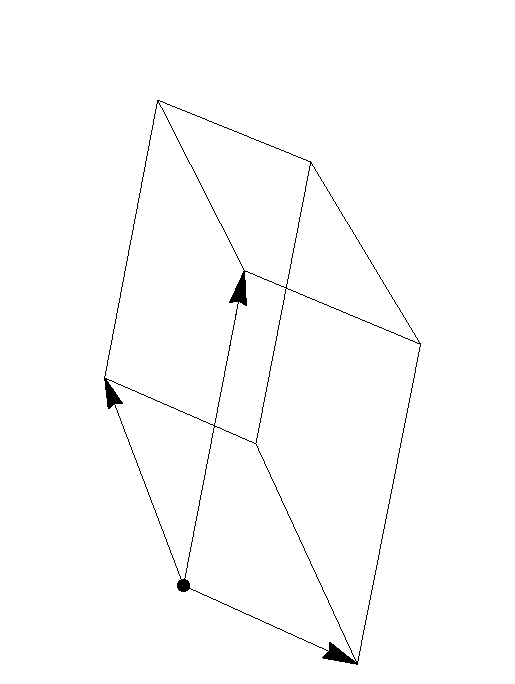
\includegraphics[width=\marginparwidth]{02-Linear-Algebra-Arithmetic/support/det}

The determinant of a 3 by 3 matrix gives the volume of the parallelepiped created by using the columns of the matrix as the three parallel edges.} 
For a 3 by 3 matrix, the columns give the edges of a three dimensional parallelepiped and the determinant produces the volume of this object. The sign of the determinant is related to orientation. If you can use your right hand and place your index finger on the first vector, middle finger on the second vector, and thumb on the third vector, then the determinant is positive. 
\begin{example}
Consider the matrix $A = \begin{bmatrix}\cl{1\\0\\0}&\cl{0\\2\\0}&\cl{0\\0\\3}\end{bmatrix}$.  Starting from the origin, each column represents an edge of the rectangular box 
$0\leq x\leq 1$, 
$0\leq y\leq 2$, 
$0\leq z\leq 3$ with volume (and determinant) $V=lwh=(1)(2)(3)=6$. The sign of the determinant is positive because if you place your index finger pointing in the direction (1,0,0) and your middle finger in the direction (0,2,0), then your thumb points upwards in the direction (0,0,3). 
If you interchange two of the columns, for example 
$B = \begin{bmatrix}\cl{0\\2\\0}&\cl{1\\0\\0}&\cl{0\\0\\3}\end{bmatrix}$, then the volume doesn't change since the shape is still the same. However, the sign of the determinant is negative because if you point your index finger in the direction (0,2,0) and your middle finger in the direction (1,0,0), then your thumb points down in the direction (0,0,-3). If you repeat this with your left hand instead of right hand, then your thumb points up.
\end{example}

\subsection{Zero Determinants and Linear Dependence}
Because the determinant helps us find area in 2D, we can use this idea to help us understand when two vectors in 2D are linearly dependent.  
If two vectors are dependent, then one is a linear combination of the other, hence a multiple of the other.  
This means that the parallelogram formed by the two vectors has no area (as the two vectors lie on the same line).  
So if the vectors are dependent, the determinant is zero.  
Similarly, if the determinant is zero, then the vectors must lie on the same line and hence are linearly dependent.  
In 3D, three vectors being linearly dependent implies that one of the vectors lies in a plane or line spanned by the other two.
Any object in 3D that lies in a plane or line has no volume so the determinant is zero.  
Similarly, if the determinant of a 3 by 3 matrix is zero, then the column vectors must lie in the same plane and hence are linearly dependent. 
We now have a geometric interpretation for the key fact that
\marginpar{For a square matrix $A$, the following are equivalent:
\begin{enumerate}
	\item The determinant is zero.
	\item The columns are linearly dependent.
	\item The rref of $A$ is not $I$.
\end{enumerate}
}
\begin{quote}The determinant of a matrix is zero if and only if the columns are linearly dependent.\end{quote}
The homeworks asks you to compute determinants of matrices as well as row reduce them so that you can verify this fact in various settings. 
Notice that the columns of a square matrix are linearly independent if and only if the reduced row echelon form of the matrix is the identity matrix. 
This shows us that the determinant of a square matrix is nonzero if and only if the reduced row echelon form of the matrix is the identity matrix. 




\section{The Matrix Inverse}
Recall that the identity matrix $I$ behaves in matrix multiplication like the number 1 behaves in regular multiplication.  
When we solve the equation $ax=b$ with numbers, we multiply both sides by $a^{-1}$ to obtain $x=a^{-1}b=\frac{1}{a}b$. 
The multiplicative inverse of $a$ is simply $1/a$, because $a\frac1a=\frac1a a=1$.
We have been studying linear systems of the form {$A\vec x=\vec b$}. 
It would be nice if we could just divide both sides by {$A$}, but there is no such thing as division by a matrix in general. 
If we look only at square matrices, then sometimes it is possible to find a matrix {$B$} such that {$BA=AB=I$}, the identity matrix. 
If such a matrix {$B$} exists, then multiplying both sides of {$A\vec x = \vec b$} on the left by the matrix {$B$} yields $BA\vec x = B\vec B$, or $I\vec x = \vec x = B\vec b$. The matrix {$B$} is then called the inverse of {$A$}, and we write it as $A^{-1}$, the same symbol we used with regular multiplication. \marginpar{The solution to $A\vec x= \vec b$ is $\vec x=A^{-1}\vec b$, provided $A^{-1}$ exists.}When an inverse exists, the solution to $A\vec x = \vec b$ is simply $\vec x = A^{-1}\vec b$.

To find an inverse, we will start by considering a general 3 by 3 matrix. Once we are done, we will know how to find the inverse of any $n$ by $n$ matrix or state it does not exists.  
If an inverse exists, then write $A^{-1} = \begin{bmatrix}
c_{11}&c_{12}&c_{13}\\ 
c_{21}&c_{22}&c_{23}\\ 
c_{31}&c_{32}&c_{33} 
\end{bmatrix} $. Then the equation $AA^{-1}=I$ requires that the 3 matrix equations
$$A\begin{bmatrix} c_{11}\\ c_{21}\\c_{31}\end{bmatrix} = \begin{bmatrix} 1\\0\\0\end{bmatrix},
A\begin{bmatrix} c_{12}\\ c_{22}\\c_{32}\end{bmatrix} = \begin{bmatrix} 0\\1\\0\end{bmatrix},
A\begin{bmatrix} c_{13}\\ c_{23}\\c_{33}\end{bmatrix} = \begin{bmatrix} 0\\ 0\\1\end{bmatrix}$$
each have a solution, or that $(1,0,0), (0,1,0),$ and  $(0,0,1)$ are all linear combinations of the columns of $A$. This requires that we reduce all three augmented matrices
$$
\begin{bmatrix}[ccc|c]
a_{11}&a_{12}&a_{13}&1\\ 
a_{21}&a_{22}&a_{23}&0\\ 
a_{31}&a_{32}&a_{33}&0 
\end{bmatrix}
\quad\quad
\begin{bmatrix}[ccc|c]
a_{11}&a_{12}&a_{13}&0\\ 
a_{21}&a_{22}&a_{23}&1\\ 
a_{31}&a_{32}&a_{33}&0 
\end{bmatrix}
\quad\quad
\begin{bmatrix}[ccc|c]
a_{11}&a_{12}&a_{13}&0\\ 
a_{21}&a_{22}&a_{23}&0\\ 
a_{31}&a_{32}&a_{33}&1 
\end{bmatrix}.
$$
If the first three columns are all pivot columns, then the row operations required to reduce all three matrices will be identical, and none of the 4th columns will be pivot columns.  Rather than do three equivalent row reductions, we can solve all three simultaneously by creating the single augmented matrix 
$$\begin{bmatrix}[ccc|ccc]
a_{11}&a_{12}&a_{13}&1&0&0\\ 
a_{21}&a_{22}&a_{23}&0&1&0\\ 
a_{31}&a_{32}&a_{33}&0&0&1 
\end{bmatrix} $$\marginpar{A matrix $A_{n\times n}$ has an inverse if
\begin{enumerate}
	\item The columns of $A$ are linearly independent.
	\item The rank of $A$ is $n$
	\item The rref of $A$ is $I$.
	\item $|A|\neq 0$.
\end{enumerate}

It does not have an inverse if
\begin{enumerate}
	\item The columns of $A$ are linearly dependent.
	\item The rank is less than $n$
	\item The rref of $A$ is not $I$ (there is a row of zeros along the bottom).
	\item $|A|=0$.
\end{enumerate}
}or in compact form $\begin{bmatrix}[c|c]A &I\end{bmatrix}$. We now reduce this larger matrix to reduced row echelon form and obtain $\begin{bmatrix}[c|c]I &B\end{bmatrix}$, which tells us the coordinates of $(1,0,0)$, $(0,1,0),$ and  $(0,0,1)$ relative to the columns of $A$. 
The columns of the augmented portion $B$ on the right are the solutions to the three original systems, hence are the columns of $A^{-1}$.
To summarize, an inverse exists precisely if the augmented system $[A|I]$ reduces to $[I|A^{-1}]$. 
The the inverse matrix appears on the right after row reduction, provided the identity matrix appears on the left.
If the left block of the augmented matrix does not reduce to the identity matrix, then the matrix does not have an inverse.
If the left block does not reduce to the identity, then this implies that the original columns of $A$ are dependent.  
Later we will show that having an inverse is equivalent to having a nonzero determinant and having a rank which equals the number of columns. Remember that this is true for square matrices, or systems where we have the same number of equations as unknowns.

\begin{example}\label{ex inverse}
To find the inverse of 
$\begin{bmatrix} 1&2\\3&4\end{bmatrix}$ 
we reduce 
$\begin{bmatrix}[cc|cc] 1&2&1&0\\3&4&0&1\end{bmatrix}$.  
Reduction gives 
$\begin{bmatrix}[cc|cc] 1&0&-2&1\\0&1&3/2&-1/2
\end{bmatrix}$. 
The inverse is the right block  
$ \begin{bmatrix} -2&1\\3/2&-1/2
\end{bmatrix}$. 
\marginpar{Examples involving larger matrices are in the homework. Remember that you can solve systems by finding an inverse of the coefficient matrix.}
You can always check your result by computing $AA^{-1}$ to see if it is $I$, for example
$\begin{bmatrix} 1&2\\ 3&4\end{bmatrix} \begin{bmatrix} -2&1\\3/2&-1/2\end{bmatrix} 
=  \begin{bmatrix} 1&0\\0&1
\end{bmatrix}$. 
Using this inverse, the solution to the system 
$\begin{cases}1x+2y=4\\3x+4y=0\end{cases}$ is $A^{-1}\vec b 
= \begin{bmatrix} -2&1\\3/2&-1/2\end{bmatrix}
\begin{bmatrix}4\\0\end{bmatrix} 
=  \begin{bmatrix}-8\\6\end{bmatrix}$.
\end{example}


\section{Eigenvalues and Eigenvectors}
Let's start by looking at an example to motivate the language we are about to introduce.  Consider the matrix
$A=\begin{bmatrix} 2&1\\1&2\end{bmatrix} $.  When we multiply this matrix by the vector 
$\vec x = \begin{bmatrix} 1\\1\end{bmatrix} $, 
we obtain 
$\begin{bmatrix} 2&1\\1&2\end{bmatrix} \begin{bmatrix} 1\\1\end{bmatrix} = \begin{bmatrix} 3\\3\end{bmatrix}=3\vec x$. Multiplication by the matrix $A$ was miraculously the same as multiplying by the number 3. Symbolically we have $A\vec x = 3\vec x$. 
Not every vector $\vec x$ satisfies this property, for by 
$\vec x = \begin{bmatrix} 1\\0\end{bmatrix} $ 
gives  
$\begin{bmatrix} 2&1\\1&2\end{bmatrix} \begin{bmatrix} 1\\0\end{bmatrix} = \begin{bmatrix} 2\\1\end{bmatrix}$, which is not a multiple of $\vec x = \begin{bmatrix} 1\\0\end{bmatrix} $. Our main goal in this section is to answer the following two questions:
\begin{enumerate}
	\item For which nonzero vectors $\vec x$ (eigenvectors) is it possible to write $A\vec x = \lambda \vec x$?
	\item Which scalars $\lambda$ (eigenvalues) satisfy $A\vec x = \lambda \vec x$?
\end{enumerate}

Now for some definitions. 
Let $A$ be a square $n\times n$ matrix. 
An eigenvector \marginpar{eigenvector}is a nonzero vector $\vec x$ such that $A\vec x =\lambda \vec x$ (matrix multiplication reduces to scalar multiplication) for some scalar {$\lambda$} called an eigenvalue.\marginpar{eigenvalue}  
We avoid letting $\vec x$ be the zero vector because $A\vec 0=\lambda \vec 0$ no matter what $\lambda$ is.
We can rewrite the equation $A\vec x = \lambda \vec x$ as $\vec 0 = A\vec x-\lambda \vec x = A\vec x-\lambda I \vec x$ and then factor to obtain $$(A-\lambda I)\vec x=\vec 0.$$ 
In other words, we need to find a $\lambda$ so that there are nonzero solutions to the homogeneous system of equations, or equivalently we need to pick a $\lambda$ so that the columns of $A-\lambda I$ are linearly dependent. 
With the correct $\lambda$, we know that $A-\lambda I$ has no inverse, and so it also means that $\det(A-\lambda I)=0$. 
This last equation is the key equation we will solve, since it does not contain the vector $\vec x$ anymore. 
The expression {$\det(A-\lambda I)$} is called the characteristic polynomial of {$A$}.
\marginpar{characteristic polynomial}
It is a polynomial of degree {$n$}, and hence there are at most {$n$} eigenvalues (which correspond to the zeros of the polynomial). 
To find the eigenvalues and eigenvectors, we 
\begin{enumerate}
	\item solve $\det(A-\lambda I) = 0$ to obtain the eigenvalues, and then
	\item for each eigenvalue, we solve $(A-\lambda I)\vec x=\vec 0$ to obtain the eigenvectors.
\end{enumerate}
As a way to check your work, the following two facts can help.
\begin{itemize}
	\item \marginpar{The trace and determinant are equal to the sum and product of the eigenvalues.
	}The sum of the eigenvalues equals the trace of the matrix (the sum of the diagonal elements).
	\item The product of the eigenvalues equals the determinant.
\end{itemize}

\begin{example} \label{ex eigen1}
To find the eigenvalues of {$\begin{bmatrix} 2&1\\1&2\end{bmatrix} $}, first subtract $\lambda$ from each diagonal entry {$\begin{bmatrix} 2-\lambda&1\\1&2-\lambda\end{bmatrix} $}, and then find the determinant. Factor to get {$(2-\lambda)(2-\lambda)-1 = \lambda^2-4\lambda+3=(\lambda-1)(\lambda-3)$}. The zeros are 1 and 3, so the eigenvalues are {$\lambda=1,3$}. As a check, the trace of this matrix is $2+2=4$ and the sum of the eigenvalues is $1+3$. In addition, the determinant is $4-1=3$ which equals the product of the eigenvalues.  

When {$\lambda=1$}, we compute {$A-\lambda I =\begin{bmatrix} 1&1\\1&1\end{bmatrix} $}. We solve the equation  {$(A-\lambda I )\vec x=0$} by reducing the augmented matrix $\begin{bmatrix}[cc|c] 1&1&0\\1&1&0\end{bmatrix} $ to its rref $\begin{bmatrix}[cc|c] 1&1&0\\0&0&0\end{bmatrix} $.\marginpar{Since we are solving a homogeneous system $A\vec x = \vec 0$, we could avoid writing the last column of zeros.} Since $x_2$ is a free variable, we solve $x_1+x_2=0$ for $x_1$ to obtain the equations $x_1=-x_2$, $x_2=x_2$, and then write our solution in vector form 
$\begin{bmatrix} x_1\\x_2\end{bmatrix}= x_2\begin{bmatrix} -1\\1\end{bmatrix}$
 for some {$x_2\neq 0$} . There are infinitely many eigenvectors corresponding to $\lambda=1$. A particular eigenvector is  $\begin{bmatrix} -1\\1\end{bmatrix} $ and all the rest are a linear combination of this one. 

When {$\lambda=3$}, we compute {$A-\lambda I =\begin{bmatrix} -1&1\\1&-1\end{bmatrix} $}. Reducing  
$\begin{bmatrix}[cc|c] -1&1&0\\1&-1&0\end{bmatrix}$ gives
$\begin{bmatrix}[cc|c] 1&-1&0\\0&0&0\end{bmatrix}$, which means the eigenvectors are of the form $x_2\begin{bmatrix} 1\\1\end{bmatrix} $ for some {$x_2\neq 0$}. A particular eigenvector corresponding to $\lambda=3$ is $\begin{bmatrix} 1\\1\end{bmatrix} $, and all others are a linear combination of this one.
\end{example}

Finding eigenvalues and eigenvectors requires that we compute determinants, find zeros of polynomials, and then solve homogeneous systems of equations. You know you are doing the problem correctly if you get infinitely many solutions to the system $(A-\lambda I)\vec x=0$ for each lambda (i.e. there is at least one row of zeros along the bottom).

Eigenvalues and eigenvectors show up in many different places in engineering, computer science, physics, chemistry, and mathematics. We will be exploring how eigenvectors appear throughout linear algebra 
%and differential equations 
as the semester progresses.  For now we'll just focus on being able to find them.

\begin{example}\label{eigenvalueexample3} \label{ex eigen2}
Let's find the eigenvalues and eigenvectors of the matrix 
$A=\begin{bmatrix}2&1&4\\ 1&2&4\\ 0&0&1\end{bmatrix}$. 
Subtracting $\lambda$ from the diagonals gives 
$\begin{bmatrix}2-\lambda&1&4\\ 1&2-\lambda&4\\ 0&0&1-\lambda\end{bmatrix}$. The determinant of this matrix is easiest to compute if you expand along the third row to get $0 - 0 + (1-\lambda) \begin{vmatrix} 2-\lambda&1\\1&2-\lambda\end{vmatrix}$. Computing the 2 by 2 determinant gives $(1-\lambda)[(2-\lambda)(2-\lambda)-1] = (1-\lambda)(\lambda-1)(\lambda-3)$,  so the eigenvalues are $1,1,3$ (1 is a repeated root). As a check, their sum is $1+1+3=5$ and the trace of $A$ is $2+2+1=5$ as well. For larger matrices, determinants are not always easy to check, so just checking the trace is a fast way to make sure you are on the right path.

When $\lambda=1$, we compute $A-\lambda I =\begin{bmatrix}1&1&4\\ 1&1&4\\ 0&0&0\end{bmatrix} $. Reducing the system  $(A-\lambda I )\vec x=0$ yields $\begin{bmatrix}[ccc|c]1&1&4&0\\ 0&0&0&0\\ 0&0&0&0\end{bmatrix}$, which has two free variables. The solution is $\begin{bmatrix} x_1\\x_2\\ x_3\end{bmatrix} = x_2\begin{bmatrix} -1\\1\\0\end{bmatrix}+x_3\begin{bmatrix} -4\\0\\1\end{bmatrix} $. Hence the eigenvectors are nonzero linear combinations of $\begin{bmatrix} -1\\1\\0\end{bmatrix}$ and $\begin{bmatrix} -4\\0\\1\end{bmatrix}$. Notice that all the eigenvectors can be obtained as linear combinations of two linearly independent eigenvectors, in part because $\lambda =1$ is a double root of the characteristic polynomial. 

When $\lambda=3$, we compute $A-\lambda I =\begin{bmatrix}-1&1&4\\ 1&-1&4\\ 0&0&-2\end{bmatrix}$. Next, reducing $\begin{bmatrix}[ccc|c]-1&1&4&0\\ 1&-1&4&0\\ 0&0&-2&0\end{bmatrix}$ yields $\begin{bmatrix}[ccc|c]-1&1&0&0\\ 0&0&1&0\\ 0&0&0&0\end{bmatrix} $, which has only one free variable . The solution is $\begin{bmatrix} x_1\\x_2\\ x_3\end{bmatrix} = x_2\begin{bmatrix} 1\\1\\0\end{bmatrix}$. The eigenvectors are nonzero linear combinations of $\begin{bmatrix} 1\\1\\0\end{bmatrix}$. Because $\lambda=3$ is a single root of the characteristic polynomial, all the eigenvectors can be obtained as linear combinations of one eigenvector.
\end{example}

\newgeometry{left=1in,right=1in,top=1in,bottom=1in}
\newpage

\section{Preparation}

\noindent
This chapter covers the following ideas. When you create your lesson plan, it should contain examples which illustrate these key ideas. Before you take the quiz on this unit, meet with another student out of class and teach each other from the examples on your lesson plan. 


\begin{enumerate}

\item Be able to use and understand matrix and vector notation, addition, scalar multiplication, the dot product, matrix multiplication, and matrix transposing. 
\item Use Gaussian elimination to solve systems of linear equations. Define and use the words homogeneous, nonhomogeneous, row echelon form, and reduced row echelon form. 
\item Find the rank of a matrix. Determine if a collection of vectors is linearly independent. If linearly dependent, be able to write vectors as linear combinations of the preceding vectors.
\item For square matrices, compute determinants, inverses, eigenvalues, and eigenvectors. 
\item Illustrate with examples how a nonzero determinant is equivalent to having independent columns, an inverse, and nonzero eigenvalues. Similarly a zero determinant is equivalent to having dependent columns, no inverse, and a zero eigenvalue. 

\end{enumerate}

The next unit will focus on applications of these ideas. The main goal of this unit is to familiarize yourself with the arithmetic involved in linear algebra.


Here are the preparation problems for this unit.  All of these problems come from this book (not Schaum's Outlines).  Remember that solutions appear at the end of each chapter.

%Day 1 we'll only look at matrix multiplication in class.  I'll introduce vector addition, scalar multiplication, the dot product, and then go to linear combinations. This leads immediately to matrix multiplication. Next we will focus on systems of equations and how to solve them.  I'll show how systems can be written in 4 ways, and then reduce a 2 by 2 system.  The next day we will focus on larger systems, and introduce rank and independence.  The next day I'll add in determinants and inverses, and hopefully get to eigenvalues and eigenvectors.   


\begin{center}
\begin{tabular}{ll|l}
\multicolumn{2}{c}{Preparation Problems (\href{http://ilearn.byui.edu/bbcswebdav/institution/Physical\_Sci\_Eng/Mathematics/Personal\%20Folders/WoodruffB/341/1-Arithmetic-Preparation-Solutions.pdf}{click for solutions})}
&
Webcasts 
(
\href{http://ilearn.byui.edu/bbcswebdav/institution/Physical\_Sci\_Eng/Mathematics/Personal\%20Folders/WoodruffB/341/1-Arithmetic-videos.pdf}{pdf copy}
)\\
\hline\hline
Day 1&
2h,
3b,
4c,
4e
&
\href{http://ilearn.byui.edu/bbcswebdav/institution/Physical\_Sci\_Eng/Mathematics/Personal\%20Folders/WoodruffB/341/1-Arithmetic-video-01.wmv}{1},
\href{http://ilearn.byui.edu/bbcswebdav/institution/Physical\_Sci\_Eng/Mathematics/Personal\%20Folders/WoodruffB/341/1-Arithmetic-video-02.wmv}{2},
\href{http://ilearn.byui.edu/bbcswebdav/institution/Physical\_Sci\_Eng/Mathematics/Personal\%20Folders/WoodruffB/341/1-Arithmetic-video-03.wmv}{3}
\\ \hline
Day 2&
4f,
5c,
6a,
6b
&
\href{http://ilearn.byui.edu/bbcswebdav/institution/Physical\_Sci\_Eng/Mathematics/Personal\%20Folders/WoodruffB/341/1-Arithmetic-video-04.wmv}{4},
\href{http://ilearn.byui.edu/bbcswebdav/institution/Physical\_Sci\_Eng/Mathematics/Personal\%20Folders/WoodruffB/341/1-Arithmetic-video-05.wmv}{5},
\href{http://ilearn.byui.edu/bbcswebdav/institution/Physical\_Sci\_Eng/Mathematics/Personal\%20Folders/WoodruffB/341/1-Arithmetic-video-06.wmv}{6}
\\ \hline
Day 3&
7d,
7h,
8b,
8j
&
\href{http://ilearn.byui.edu/bbcswebdav/institution/Physical\_Sci\_Eng/Mathematics/Personal\%20Folders/WoodruffB/341/1-Arithmetic-video-07.wmv}{7},
\href{http://ilearn.byui.edu/bbcswebdav/institution/Physical\_Sci\_Eng/Mathematics/Personal\%20Folders/WoodruffB/341/1-Arithmetic-video-08.wmv}{8}
\\ \hline
Day 4&
9b,
10e,
10g,
10h
&
\href{http://ilearn.byui.edu/bbcswebdav/institution/Physical\_Sci\_Eng/Mathematics/Personal\%20Folders/WoodruffB/341/1-Arithmetic-video-09.wmv}{9},
\href{http://ilearn.byui.edu/bbcswebdav/institution/Physical\_Sci\_Eng/Mathematics/Personal\%20Folders/WoodruffB/341/1-Arithmetic-video-10.wmv}{10},
\href{http://ilearn.byui.edu/bbcswebdav/institution/Physical\_Sci\_Eng/Mathematics/Personal\%20Folders/WoodruffB/341/1-Arithmetic-video-11.wmv}{11}
\\ \hline
Day 5&
11, 
Lesson Plan,
Quiz &
\\ \hline
\end{tabular}
\end{center}

Please download and print all the problems. I have tried to keep the text short and readable, and I want you to read the text (reading 3-4 pages for every day of class will get you through the whole book). If you find errors or find some parts hard to read, please email me so that I can improve the text.




The problems listed below are found in the subsequent pages. The suggested problems are a minimal set of problems that I suggest you complete.
\begin{center}
\begin{tabular}{|l|l|l|l|l|}
\hline
Concept&Suggestions&Relevant Problems\\ \hline
Basic Notation&1bcf,2abehln&1,2\\ \hline
Gaussian Elimination&3all,4acf&3,4\\ \hline
Rank and Independence&5ac,6bd&5,6\\ \hline
Determinants&7adgh&7\\ \hline
Inverses&8ag,9ac&8,9\\ \hline
Eigenvalues&10abdghi&10\\ \hline
Summarize&11(multiple times)&11\\ \hline
\end{tabular}
\end{center}






\section{Problems}


\begin{enumerate}


\item \textbf{Vector Arithmetic:} For each pair of vectors, (1) find the length of each vector, (2) compute the dot product of the vectors, (3) find the cosine of the angle between them, and (4) determine if the vectors are orthogonal.
\begin{enumerate}
\begin{multicols}{3}
	\item $(1,2), (3,4)$
	\item $[-2~1], [4~-8]$
	\item $(1,2,2), (3,0,-4)$
	\item $\left<-2,3,5\right>, \left<4,-4,4\right>$
	\item $[1~1~1~1], [2~3~-4~-1]$
	\item $[1~-4~3~0~2]^T, [2~1~0~10~1]^T$
\end{multicols}
\end{enumerate}
%More problems are in Schaum's Outlines - 
%Chapter 1:1-13,  54-66.
\item \textbf{Matrix Arithmetic:} Consider the matrices
$$
A=
\begin{bmatrix}
 1 & 2 \\
 3 & 4
\end{bmatrix}
,
B=
\begin{bmatrix}
 4 & -1 \\
 3 & 2
\end{bmatrix}
,
C=
\begin{bmatrix}
 1 & 0 & -1 \\
 2 & 3 & 4
\end{bmatrix}
,
D=
\begin{bmatrix}
 0 & 2 & 1 \\
 3 & 0 & 4 \\
 -1 & 1 & 2
\end{bmatrix}
, \text{ and }
E=
\begin{bmatrix}
 3 \\
 1 \\
 -4
\end{bmatrix}.
$$
Compute each of the following, or explain why it is not possible.
\begin{enumerate}
\begin{multicols}{4}
	\item $A+B$ and $3A-2B$
	\item $AB$ and $BA$
	\item $AC$ and $CA$
	\item $BC$ and $CB$
	\item $CD$ and $DC$
	\item $DE$ and $ED$
	\item $CDE$
	\item $CC^T$ and $C^TC$
	\item $DC^T$ and $CD^T$
	\item $AB$ and $B^TA^T$
	\item $BA$ and $A^TB^T$
	\item Trace of $A$, $B$, $D$.	
\end{multicols}
\end{enumerate}
For each of the following, compute the product in three ways (1) using linear combinations of columns, (2) using rows dotted by columns, and (3) using linear combinations of rows (see Table \ref{matrixmult}).
\begin{multicols}{4}
\begin{enumerate}[resume]
\item $AB$
\item $BC$
\item $CD$
\item $DE$
\end{enumerate}
\end{multicols}
%More problems are in Schaum's Outlines - 
%Chapter 1:14-26, 67-79;
%Chapter 3:1-3, 68-70.






\item \textbf{Interpreting RREF:} Each of the following augmented matrices requires one row operation to be in reduced row echelon form. Perform the required row operation, and then write the solution to corresponding system of equations in terms of the free variables.
\begin{multicols}{3}
\begin{enumerate}
	\item 
$
\begin{bmatrix}[ccc|c]
 1 & 0 & 0 & 3 \\
 0 & 0 & 1 & 1 \\
 0 & 1 & 0 & -2
\end{bmatrix}
$
	\item 
$
\begin{bmatrix}[ccc|c]
 1 & 2 & 0 & -4 \\
 0 & 0 & 1 & 3 \\
 -3 & -6 & 0 & 12
\end{bmatrix}
$
	\item 
$
\begin{bmatrix}[ccc|c]
 0 & 1 & 0 & 4 \\
 0 & 0 & 5 & 15 \\
 0 & 0 & 0 & 0
\end{bmatrix}
$
	\item 
$
\begin{bmatrix}[ccc|c]
 1 & 0 & 2 & 4 \\
 0 & 1 & -3 & 0 \\
 0 & 0 & 0 & 1
\end{bmatrix}
$
	\item 
$
\begin{bmatrix}[ccccc|c]
 0 & 1 & 0 & 7 & 0 & 3 \\
 0 & 0 & 1 & 5 & -3 & -10 \\
 0 & 0 & 0 & 0 & 1 & 2 \\
 0 & 0 & 0 & 0 & 0 & 0
\end{bmatrix}
$
\end{enumerate}
\end{multicols}

%More problems are in Schaum's Outlines - 
%Chapter 2:37-40


\item \textbf{Solving Systems with Gaussian Elimination:} Solve each system of equations using Gaussian elimination, by reducing the augmented matrix to reduced row echelon form (rref).
\begin{multicols}{3}
\begin{enumerate}
	\item 
$
\begin{array}{rl}
 x  -3y &= 10 \\
 3x +2y &= 8
\end{array}
$


	\item 
$
\begin{array}{rl}
 2x+ 6y -z &= 9 \\
 x+ 3y -3z &= 17
\end{array}
$


	\item 
$
\begin{array}{rl}
  x_2 -2x_3 &= -5 \\
 2x_1 -x_2 + 3x_3 &= 4 \\
 4x_1 +x_2 + 4x_3 &= 5
\end{array}
$


	\item 
$
\begin{array}{rl}
 x_1 + 2x_3 &= -2 \\
 2x_1  -3x_2  &= -3 \\
 3x_1 +x_2 -x_3 &= 2
\end{array}
$


	\item 
$
\begin{array}{rl}
 2x_1 +x_2 + 4x_3 &= -1 \\
 -x_1 + 3x_2 + 5x_3 &= 2 \\
 x_2 + 2x_3 &= -2
\end{array}
$


	\item 
$
\begin{array}{rl}
 x_1 -2x_2 +x_3 &= 4 \\
 -x_1 + 2x_2 + 3x_3 &= 8 \\
 2x_1  -4x_2 +x_3 &= 5
\end{array}
$


	\item 
$
\begin{array}{rl}
 x_1 + 2x_3 + 3x_4 &= -7 \\
 2x_1 +x_2 + 4x_4 &= -7 \\
 -x_1 + 2x_2 + 3x_3  &= 0 \\
 x_2  -2x_3  -x_4 &= 4
\end{array}
$
\end{enumerate}
\end{multicols}

%More problems are in Schaum's Outlines - 
%Chapter 2:
%44-48, 51-56, 70-72, 75-28, 86-90 






\item \textbf{Rank and Linear Dependence:} Compute the rank of each matrix. Use this result to determine if the columns are linearly dependent. If the vectors are dependent, write each non pivot column as a linear combination of the pivot columns.
\begin{multicols}{4}
\begin{enumerate}
	\item \label{rank1} 
$
\begin{bmatrix}
 1 & 2 & 3 \\
 4 & -2 & 1 \\
 3 & 0 & 4
\end{bmatrix}
$

	\item \label{rank2}
$
\begin{bmatrix}
 1 & -1 & -1 \\
 -2 & 3 & 5 \\
 3 & 1 & 9
\end{bmatrix}
$

	\item 
$
\begin{bmatrix}
 1 & 3 & -1 & 9 \\
 -1 & -2 & 0 & -5 \\
 2 & 1 & 3 & -2
\end{bmatrix}
$

	\item \label{rank4}
$
\begin{bmatrix}
 1 & 3 & 12 & 1 \\
 2 & 0 & -6 & 3 \\
 -1 & 1 & 8 & -4 \\
 0 & 2 & 10 & 2
\end{bmatrix}
$

\end{enumerate}
\end{multicols}

%More problems are in Schaum's Outlines - 
%Chapter 5:
%19, 20, 22, 68.





\item \textbf{Linear Independence:} In each problem, determine if the vectors given are linearly independent. If the vectors are linearly dependent, write one of the vectors as a linear combination of the others.
\begin{multicols}{2}
\begin{enumerate}
	\item \,
	$[2, -1, 0]$, $[1, 0, 3]$, $[3, 2, 4]$

	\item \,
$[1, 2, -3, 4], [3, -2, -1, -2], [5, -2, -3, -1]$

	\item \,
$[0, 1, 1, 1], [1, 0, 1, 1], [1, 1, 0, 1], [1, 1, 1, 0]$

	\item \,
$[1, 0, -1, -2], [1, 2, 3, 0], [0, 1, -1, 2], [2, 0, 1, -5]$
\end{enumerate}
\end{multicols}

%More problems are in Schaum's Outlines - 
%Chapter 5:
%1, 3, 4, 50, 53.


\item \textbf{Determinants:} Find the determinant of each matrix. For 3 by 3 matrices, compute the determinant in 2 different ways by using a cofactor expansion along a different row or column. 
\begin{enumerate}
\begin{multicols}{3}
	\item 
$
\begin{bmatrix}
 1 & 2 \\
 3 & 4
\end{bmatrix}
$
	\item 
$
\begin{bmatrix}
 4 & 3 \\
 5 & 9
\end{bmatrix}
$
	\item 
$
\begin{bmatrix}
 2 & 1 & 0 \\
 0 & 2 & 1 \\
 1 & 0 & 2
\end{bmatrix}
$
	\item 
$
\begin{bmatrix}
 3 & 1 & -2 \\
 1 & -1 & 4 \\
 2 & 2 & 1
\end{bmatrix}
$
	\item 
$
\begin{bmatrix}
 2 & 3 & -1 \\
 1 & 0 & 0 \\
 4 & 2 & 5
\end{bmatrix}
$
	\item 
$
\begin{bmatrix}
 5 & 1 & -3 \\
 2 & -1 & 2 \\
 1 & 4 & -1
\end{bmatrix}
$
	\item 
$
\begin{bmatrix}
 2 & 1 & -6 & 8 \\
 0 & 3 & 5 & 4 \\
 0 & 0 & 1 & 5 \\
 0 & 0 & 0 & -4
\end{bmatrix}
$
	\item 
$
\begin{bmatrix}
 3 & 2 & 5 & -1 \\
 0 & 8 & 4 & 2 \\
 0 & -1 & 0 & 0 \\
 0 & -5 & 3 & -1
\end{bmatrix}
$
	\item 
$
\begin{bmatrix}
 1 & 1 & 1 & 1 \\
 2 & -1 & 1 & 1 \\
 -1 & 1 & 2 & -2 \\
 1 & 1 & -1 & -1
\end{bmatrix}
$
	\item 
$
\begin{bmatrix}
 1 & 1 & 1 & 1 \\
 2 & 2 & 2 & 2 \\
 0 & 2 & 1 & -1 \\
 1 & 0 & -2 & 1
\end{bmatrix}
$
\end{multicols}
\end{enumerate}

For the following matrices, compute the determinant and use your answer to determine if the columns are linearly independent.
\begin{enumerate}[resume]
\begin{multicols}{3}
	\item Use the matrix from \ref{rank1}
	\item Use the matrix from \ref{rank2}
	\item Use the matrix from \ref{rank4}
\end{multicols}
\end{enumerate}

%More problems are in Schaum's Outlines -  
%Chapter 10:
%1-6, 21, 23, 51-55






\item \textbf{Inverse:} Find the inverse of each matrix below.
\begin{multicols}{4}
\begin{enumerate}
	\item \label{inv1}
$
\begin{bmatrix}
 1 & 2 \\
 3 & 4
\end{bmatrix}
$
	\item \label{inv2}
$
\begin{bmatrix}
 -2 & 4 \\
 3 & -5
\end{bmatrix}
$
	\item 
$
\begin{bmatrix}
 0 & 1 \\
 -1 & 0
\end{bmatrix}
$
	\item 
$
\begin{bmatrix}
 2 & 3 \\
 4 & 5
\end{bmatrix}
$
	\item 
$
\begin{bmatrix}
 7 & 3 \\
 2 & 1
\end{bmatrix}
$
	\item 
$
\begin{bmatrix}
 1 & 0 & 2 \\
 0 & 1 & 0 \\
 0 & 0 & 4
\end{bmatrix}
$
	\item \label{inv3}
$
\begin{bmatrix}
 1 & 0 & 2 \\
 0 & 1 & 0 \\
 -1 & 1 & 4
\end{bmatrix}
$
	\item 
$
\begin{bmatrix}
 3 & 0 & 3 \\
 0 & -1 & 1 \\
 0 & 3 & -4
\end{bmatrix}
$
	\item 
$
\begin{bmatrix}
 1 & 2 & -1 \\
 2 & 3 & -2 \\
 0 & 3 & 2
\end{bmatrix}
$
	\item \label{inv4}
$
\begin{bmatrix}
 -2 & 0 & 5 \\
 -1 & 0 & 3 \\
 4 & 1 & -1
\end{bmatrix}
$
	\item 
$
\begin{bmatrix}
 2 & 1 & 1 \\
 1 & 2 & 1 \\
 1 & 1 & 2
\end{bmatrix}
$
	\item 
$
\begin{bmatrix}
a & b\\
c & d
\end{bmatrix}
$
\end{enumerate}
\end{multicols}




%More problems are in Schaum's Oultines:
%Chapter 3: 7-11, 77-80.


\item \textbf{Solve systems using an inverse:} Solve each system by using an inverse from above.
\begin{multicols}{2}
\begin{enumerate}
	\item 
$\left\{
\begin{array}{rl}
 x_1 + 2x_2  &=3\\
 3x_1 + 4x_2  &=4
\end{array}
\right.$ using \ref{inv1}.
	\item 
$\left\{
\begin{array}{rl}
 -2x_1 + 4x_2  &=4\\
 3x_1  -5x_2  &=-2
\end{array}
\right.$ using \ref{inv2}.
	\item 
$\left\{
\begin{array}{rl}
 1x_1 + 2x_3 &=2\\
 x_2 &=3\\
 -x_1 +x_2 + 4x_3  &=1
\end{array}
\right.$ using \ref{inv3}.
	\item 
$\left\{
\begin{array}{rl}
 -2x_1+ 5x_3 &=-2\\
 -x_1+ 3x_3 &=1\\
 4x_1 +x_2  -x_3 &=3
\end{array}
\right.$ using \ref{inv4}.
\end{enumerate}
\end{multicols}

Now grab any problem from the entire unit that involves solving a system where an inverse applies.  Find the inverse of the coefficient matrix and use it to find the solution. (Use the solutions at the back to select a problem with a unique solution).



\item \textbf{Eigenvalues and Eigenvectors:} For each matrix, compute the characteristic polynomial and eigenvalues. For each eigenvalue, give all the corresponding eigenvectors. Remember that you can check your answer by comparing the trace to the sum of the eigenvalues, and the determinant to the product of the eigenvalues.
\begin{multicols}{4}
\begin{enumerate}
	\item 
$
\begin{bmatrix}
 1 & 2 \\
 0 & 3
\end{bmatrix}
$
	\item 
$
\begin{bmatrix}
 0 & 1 \\
 -1 & -2
\end{bmatrix}
$
	\item 
$
\begin{bmatrix}
 2 & 3 \\
 3 & 2
\end{bmatrix}
$
	\item 
$
\begin{bmatrix}
 0 & 1 \\
 -1 & 0
\end{bmatrix}
$
	\item 
$
\begin{bmatrix}
 1 & 4 \\
 2 & 3
\end{bmatrix}
$
	\item 
$
\begin{bmatrix}
 3 & 1 \\
 4 & 6
\end{bmatrix}
$
	\item 
$
\begin{bmatrix}
 1 & 2 & 2 \\
 0 & 1 & 2 \\
 0 & 0 & 1
\end{bmatrix}
$
	\item 
$
\begin{bmatrix}
 1 & 2 & 2 \\
 0 & 1 & 0 \\
 0 & 0 & 1
\end{bmatrix}
$
	\item 
$
\begin{bmatrix}
 3 & 0 & 0 \\
 0 & 2 & 1 \\
 0 & 1 & 2
\end{bmatrix}
$
	\item 
$
\begin{bmatrix}
 1 & 1 & 0 \\
 0 & 2 & 0 \\
 0 & 1 & 1
\end{bmatrix}
$
\end{enumerate}
\end{multicols}
 
%More problems are in Schaum's Outlines - 
%(only worry about the eigenvalues and eigenvectors part of each problem - ignore diagonalization questions)
%Chapter 11: 9, 10, 11, 17, 18, 20, 57, 58, 59, 60



\item At this point, you are ready to make your own examples. Create your own 2 by 2 or 3 by 3 matrix $A$.
\begin{itemize}
\begin{multicols}{2}
	\item Find rref $A$.
	\item Find the rank of $A$.
	\item Are the columns of $A$ independent?
	\item Compute $|A|$.
	\item Compute $A^{-1}$ (or explain why not possible).
	\item Find the eigenvalues and eigenvectors of $A$.
\end{multicols}
\end{itemize}
For a 3 by 3 matrix, the eigenvalues and eigenvectors may be hard to find by hand (so use technology).
Use technology to check your work by hand. The first column of questions applies to all matrices (square or not), whereas the last column only makes sense when the matrix is square. For a 2 by 2 matrix, you can always compute the eigenvalues using the quadratic formula, which may result in irrational or complex eigenvalues. 

Repeat this exercise a few times with various types of matrices (diagonal, triangular, symmetric, skew-symmetric). Do you notice any patterns? If you pick larger matrices, you can do everything except the eigenvalues and eigenvectors by hand. Once you feel comfortable with the computations by hand, move to a computer and start using larger matrices to find patterns. 
 


\end{enumerate}



\section{Projects}
The following projects require you to use technology to further explore a topic from this unit. Use a computer algebra system (CAS) to perform your computations so you can save your work and quickly modify things as needed. 

\begin{enumerate}
	\item A matrix and its transpose $A^T$ have some common properties. Your job in this project is to explore the relationships between a matrix and its transpose.	
	
\begin{enumerate}
	\item Start by choosing your own 4 by 4 matrix.  For both $A$ and $A^T$, compute the rref, rank, determinant, inverse, eigenvalues, and eigenvectors. Which are the same? 
	\item Change your matrix to some other 4 by 4 or larger matrix and repeat the computations. 
	\item Based on these two examples, which quantities do you think will be always be the same for $A$ and $A^T$? 
	\item Try creating an ugly large matrix and see if your conjecture is correct. While examples are not proofs that a conjecture is true, examples do provide the foundation upon which all mathematical theorems are built.  New ideas always stem from examples.
	\item What happens if a matrix is not square? Select your own non square matrix (such as 3 by 4). Compute the rref of both $A$ and $A^T$, as well as the rank. 
	\item Change the matrix and repeat this computation. What conjecture should you make?
\end{enumerate}
\end{enumerate}








\section{Solutions}




\begin{multicols}{2}
\begin{enumerate}
\small
\item \textbf{Vector Arithmetic:}
\begin{enumerate}
	\item $\sqrt{5}, 5, 11, \cos\theta = \frac{11}{5\sqrt{5}}$, No
	\item $\sqrt{5}, 2\sqrt{5}, 0, \cos\theta = 0$, Yes
	\item $3, 5, -5, \cos\theta = -\frac{1}{3}$, No
	\item $\sqrt{38}, 4\sqrt{3}, 0, \cos\theta = 0$, Yes
	\item $2, \sqrt{30}, 0, \cos\theta = 0$, Yes
	\item $\sqrt{30}, \sqrt{106}, 0, \cos\theta = 0$, Yes
\end{enumerate}
\item \textbf{Matrix Arithmetic:}
%\begin{multicols}{4}
\begin{enumerate}
	\item $ 
\begin{bmatrix}
5 & 1 \\
 6 & 6
\end{bmatrix}
$, $
\begin{bmatrix}
 -5 & 8 \\
 3 & 8
\end{bmatrix}
$
	\item 
$
\begin{bmatrix}
 10 & 3 \\
 24 & 5
\end{bmatrix}
$, 
$
\begin{bmatrix}
 1 & 4 \\
 9 & 14
\end{bmatrix}
$
	\item 
	$
\begin{bmatrix}
 5 & 6 & 7 \\
 11 & 12 & 13
\end{bmatrix}
$, $CA$ not possible
	\item 
	$
\begin{bmatrix}
 2 & -3 & -8 \\
 7 & 6 & 5
\end{bmatrix}
$, $CB$ not possible
	\item 
	$
\begin{bmatrix}
 1 & 1 & -1 \\
 5 & 8 & 22
\end{bmatrix}
$, $DC$ not possible
	\item 
	$
\begin{bmatrix}
 -2 \\
 -7 \\
 -10
\end{bmatrix}
$, $ED$ not possible
	\item $
\begin{bmatrix}
 8 \\
 -65
\end{bmatrix}
$
	\item 
$\begin{bmatrix}
 2 & -2 \\
 -2 & 29
\end{bmatrix}$, 
$
\begin{bmatrix}
 5 & 6 & 7 \\
 6 & 9 & 12 \\
 7 & 12 & 17
\end{bmatrix}
$
	\item 
$\begin{bmatrix}
 -1 & 10 \\
 -1 & 22 \\
 -3 & 9
\end{bmatrix}
$, $
\begin{bmatrix}
 -1 & -1 & -3 \\
 10 & 22 & 9
\end{bmatrix}
$	\item 
$\begin{bmatrix}
 10 & 3 \\
 24 & 5
\end{bmatrix}
$, $
\begin{bmatrix}
 10 & 24 \\
 3 & 5
\end{bmatrix}
$	
\item 
$\begin{bmatrix}
 1 & 4 \\
 9 & 14
\end{bmatrix}
$, $
\begin{bmatrix}
 1 & 9 \\
 4 & 14
\end{bmatrix}
$	\item  Tr$A=5$, Tr$B=6$, Tr$D=2$.	
\end{enumerate}
%\end{multicols}







\item \textbf{Interpreting RREF:} 
%\begin{multicols}{3}
\begin{enumerate}
	\item 
$
\begin{bmatrix}[ccc|c]
 1 & 0 & 0 & 3 \\
 0 & 1 & 0 & -2 \\
 0 & 0 & 1 & 1
\end{bmatrix}$,
$\begin{array}{rl}
x_1&=3\\ 
x_2&=-2\\
x_3&=1
\end{array}$
	\item 
$
\begin{bmatrix}[ccc|c]
 1 & 2 & 0 & -4 \\
 0 & 0 & 1 & 3 \\
 0 & 0 & 0 & 0
\end{bmatrix}
$,
$\begin{array}{rl}
x_1&=-2x_2-4 \\
x_2&=x_2 \text{ (free variable)} \\
x_3&=3
\end{array}$


	\item 
$
\begin{bmatrix}[ccc|c]
 0 & 1 & 0 & 4 \\
 0 & 0 & 1 & 3 \\
 0 & 0 & 0 & 0
\end{bmatrix}
$,
$
\begin{array}{rl}
x_1&=x_1 \text{ (free)} \\
x_2&=4 \\
x_3&=3
\end{array}
$


	\item 
$
\begin{bmatrix}[ccc|c]
 1 & 0 & 2 & 0 \\
 0 & 1 & -3 & 0 \\
 0 & 0 & 0 & 1
\end{bmatrix}
$,
no solution


	\item 
$
\begin{bmatrix}[ccccc|c]
 0 & 1 & 0 & 7 & 0 & 3 \\
 0 & 0 & 1 & 5 & 0 & -4 \\
 0 & 0 & 0 & 0 & 1 & 2 \\
 0 & 0 & 0 & 0 & 0 & 0
\end{bmatrix}
$,
$\begin{array}{rl}
x_1&=x_1 \text{ (free)}\\
x_2&=-7x_4+3\\
x_3&=-5x_4-4\\
x_4&=x_4 \text{ (free)}\\
x_5&=2
\end{array}$


\end{enumerate}
%\end{multicols}


\item \textbf{Solving Systems with Gaussian Elimination:} 
%\begin{multicols}{3}
\begin{enumerate}
	\item 
$
\begin{bmatrix}[cc|c]
 1 & 0 & 4 \\
 0 & 1 & -2
\end{bmatrix}
$
$
\begin{array}{rl}
x_1&=4 \\
x_2&=-2 
\end{array}
$


	\item 
$
\begin{bmatrix}[ccc|c]
 1 & 3 & 0 & 2 \\
 0 & 0 & 1 & -5
\end{bmatrix}
$
$
\begin{array}{rl}
x_1&=-3x_2+2  \\
x_2&=x_2 \text{ (free)} \\
x_3&=-5
\end{array}
$


	\item 
$
\begin{bmatrix}[ccc|c]
 1 & 0 & 0 & -2 \\
 0 & 1 & 0 & 1 \\
 0 & 0 & 1 & 3
\end{bmatrix}
$
$
\begin{array}{rl}
x_1&=-2  \\
x_2&=1 \\
x_3&=3
\end{array}
$


	\item 
$
\begin{bmatrix}[ccc|c]
 1 & 0 & 0 & 0 \\
 0 & 1 & 0 & 1 \\
 0 & 0 & 1 & -1
\end{bmatrix}
$
$
\begin{array}{rl}
x_1&=0  \\
x_2&=1 \\
x_3&=-1
\end{array}
$


	\item 
$
\begin{bmatrix}[ccc|c]
 1 & 0 & 1 & 0 \\
 0 & 1 & 2 & 0 \\
 0 & 0 & 0 & 1
\end{bmatrix}
$,
no solution


	\item 
$
\begin{bmatrix}[ccc|c]
 1 & -2 & 0 & 1 \\
 0 & 0 & 1 & 3 \\
 0 & 0 & 0 & 0
\end{bmatrix}
$
$
\begin{array}{rl}
x_1&=2x_2+1  \\
x_2&=x_2 \text{ (free)} \\
x_3&=3
\end{array}
$


	\item 
$
\begin{bmatrix}[cccc|c]
 1 & 0 & 0 & 0 & 2 \\
 0 & 1 & 0 & 0 & 1 \\
 0 & 0 & 1 & 0 & 0 \\
 0 & 0 & 0 & 1 & -3
\end{bmatrix}
$
$
\begin{array}{rl}
x_1&=2  \\
x_2&=1 \\
x_3&=0\\
x_4&=-3
\end{array}
$

\end{enumerate}
%\end{multicols}







\item \textbf{Rank and Linear Dependence:}
%\begin{multicols}{4}
\begin{enumerate}
	\item 3, independent
	\item 2, dependent, 
	rref is $\begin{bmatrix}
 1 & 0 & 2 \\
 0 & 1 & 3 \\
 0 & 0 & 0
	\end{bmatrix}
	$ 
	so
	
$
2\begin{bmatrix}
 1  \\
 -2  \\
 3 
\end{bmatrix}
+3\begin{bmatrix}
 -1 \\
 3  \\
 1 
\end{bmatrix}
=\begin{bmatrix}
-1 \\
 5 \\
 9
\end{bmatrix}
$

	\item 2, dependent, rref is 
$
\begin{bmatrix}
 1 & 0 & 2 & -3 \\
 0 & 1 & -1 & 4 \\
 0 & 0 & 0 & 0
\end{bmatrix}
$ so

$
2\begin{bmatrix}
 1 \\
 -1  \\
 2 
\end{bmatrix}
-1\begin{bmatrix}
  3  \\
  -2  \\
  1 
\end{bmatrix}
=\begin{bmatrix}
-1  \\
0  \\
3 
\end{bmatrix}
$ and

$
-3\begin{bmatrix}
 1 \\
 -1  \\
 2 
\end{bmatrix}
+4\begin{bmatrix}
  3  \\
  -2  \\
  1 
\end{bmatrix}
=\begin{bmatrix}
9 \\
-5 \\
-2
\end{bmatrix}
$


	\item 3, dependent, rref is 
$
\begin{bmatrix}
 1 & 0 & -3 & 0 \\
 0 & 1 & 5 & 0 \\
 0 & 0 & 0 & 1 \\
 0 & 0 & 0 & 0
\end{bmatrix}
$ so 

$-3
\begin{bmatrix}
 1\\
 2\\
 -1\\
 0
\end{bmatrix}
+5
\begin{bmatrix}
3  \\
0 \\
1 \\
2 
\end{bmatrix}
+0
\begin{bmatrix}
 1 \\
3 \\
-4 \\
2
\end{bmatrix}
=
\begin{bmatrix}
 12 \\
 -6 \\
 8 \\
 10
\end{bmatrix}
$

\end{enumerate}
%\end{multicols}






\item \textbf{Linear Independence:} 
%\begin{multicols}{2}
\begin{enumerate}
	\item 
$
\begin{bmatrix}
 2 & 1 & 3 \\
 -1 & 0 & 2 \\
 0 & 3 & 4
\end{bmatrix}
\xrightarrow{\text{rref}}
\begin{bmatrix}
 1 & 0 & 0 \\
 0 & 1 & 0 \\
 0 & 0 & 1
\end{bmatrix}
$, 
independent

	\item 
$
\begin{bmatrix}
 1 & 3 & 5 \\
 2 & -2 & -2 \\
 -3 & -1 & -3 \\
 4 & -2 & -1
\end{bmatrix}
\rightarrow
\begin{bmatrix}
 1 & 0 & \frac{1}{2} \\
 0 & 1 & \frac{3}{2} \\
 0 & 0 & 0 \\
 0 & 0 & 0
\end{bmatrix}
$, 
dependent

$\dfrac{1}{2}\begin{bmatrix}
 1 \\
 2 \\
 -3 \\
 4 
\end{bmatrix}
+\dfrac{3}{2}
\begin{bmatrix}
3  \\
-2 \\
-1  \\
-2
\end{bmatrix}
=
\begin{bmatrix}
 5 \\
 -2 \\
-3 \\
-1
\end{bmatrix}$


	\item Independent. Placing the vectors in columns of a 4 by 4 matrix reduces to the identity, so there are 4 pivot columns.

	\item 
$
\begin{bmatrix}
 1 & 1 & 0 & 2 \\
 0 & 2 & 1 & 0 \\
 -1 & 3 & -1 & 1 \\
 -2 & 0 & 2 & -5
\end{bmatrix}
\rightarrow
\begin{bmatrix}
 1 & 0 & 0 & \frac{3}{2} \\
 0 & 1 & 0 & \frac{1}{2} \\
 0 & 0 & 1 & -1 \\
 0 & 0 & 0 & 0
\end{bmatrix}
$, 

dependent

$\dfrac{3}{2}\begin{bmatrix}
 1  \\
 0 \\
 -1  \\
 -2 
\end{bmatrix}
+\dfrac{1}{2}
\begin{bmatrix}
1 \\
2 \\
3 \\
0
\end{bmatrix}
-
\begin{bmatrix}
 0 \\
 1 \\
 -1 \\
 2 
\end{bmatrix}
=
\begin{bmatrix}
 2 \\
 0 \\
 1 \\
-5
\end{bmatrix}$



\end{enumerate}
%\end{multicols}


\item \textbf{Determinants:}
\begin{multicols}{3}
\begin{enumerate}
	\item $-2$
	\item $21$
	\item $9$
	\item $-28$
	\item $-17$
	\item $-58$
	\item $-24$
	\item $-30$
	\item $24$
	\item $0$
\end{enumerate}
\end{multicols}




\item \textbf{Inverse:}
\begin{multicols}{2}
\begin{enumerate}
	\item 
$
\begin{bmatrix}
 -2 & 1 \\
 \frac{3}{2} & -\frac{1}{2}
\end{bmatrix}
$
	\item 
$
\begin{bmatrix}
 \frac{5}{2} & 2 \\
 \frac{3}{2} & 1
\end{bmatrix}
$
	\item 
$
\begin{bmatrix}
 0 & -1 \\
 1 & 0
\end{bmatrix}
$
	\item 
$
\begin{bmatrix}
 -\frac{5}{2} & \frac{3}{2} \\
 2 & -1
\end{bmatrix}
$
	\item 
$
\begin{bmatrix}
 1 & -3 \\
 -2 & 7
\end{bmatrix}
$
	\item 
$
\begin{bmatrix}
 1 & 0 & -\frac{1}{2} \\
 0 & 1 & 0 \\
 0 & 0 & \frac{1}{4}
\end{bmatrix}
$
	\item 
$
\begin{bmatrix}
 \frac{2}{3} & \frac{1}{3} & -\frac{1}{3} \\
 0 & 1 & 0 \\
 \frac{1}{6} & -\frac{1}{6} & \frac{1}{6}
\end{bmatrix}
$
	\item 
$
\begin{bmatrix}
 \frac{1}{3} & 3 & 1 \\
 0 & -4 & -1 \\
 0 & -3 & -1
\end{bmatrix}
$
	\item 
$
\begin{bmatrix}
 -6 & \frac{7}{2} & \frac{1}{2} \\
 2 & -1 & 0 \\
 -3 & \frac{3}{2} & \frac{1}{2}
\end{bmatrix}
$
	\item 
$
\begin{bmatrix}
 -3 & 5 & 0 \\
 11 & -18 & 1 \\
 -1 & 2 & 0
\end{bmatrix}
$
	\item 
$
\begin{bmatrix}
 \frac{3}{4} & -\frac{1}{4} & -\frac{1}{4} \\
 -\frac{1}{4} & \frac{3}{4} & -\frac{1}{4} \\
 -\frac{1}{4} & -\frac{1}{4} & \frac{3}{4}
\end{bmatrix}
$
	\item 
$
\dfrac{1}{ad-bc}\begin{bmatrix}
d & -b\\
-c & a
\end{bmatrix}
$
\end{enumerate}
\end{multicols}





\item \textbf{Solve systems using an inverse:} 
%\begin{multicols}{2}
\begin{enumerate}
	\item 
$
\begin{bmatrix}
 -2 & 1 \\
 \frac{3}{2} & -\frac{1}{2}
\end{bmatrix}
\begin{bmatrix}
 3 \\
 4
\end{bmatrix}
=
\begin{bmatrix}
 -2 \\
 \frac{5}{2}
\end{bmatrix}
$

	\item 
$
\begin{bmatrix}
 \frac{5}{2} & 2 \\
 \frac{3}{2} & 1
\end{bmatrix}
\begin{bmatrix}
 4 \\
 -2
\end{bmatrix}
=
\begin{bmatrix}
 6 \\
 4
\end{bmatrix}
$


	\item 
$
\begin{bmatrix}
 \frac{2}{3} & \frac{1}{3} & -\frac{1}{3} \\
 0 & 1 & 0 \\
 \frac{1}{6} & -\frac{1}{6} & \frac{1}{6}
\end{bmatrix}
\begin{bmatrix}
 2 \\
 3 \\
 1
\end{bmatrix}
=
\begin{bmatrix}
 2 \\
 3 \\
 0
\end{bmatrix}
$


	\item 
$
\begin{bmatrix}
 -3 & 5 & 0 \\
 11 & -18 & 1 \\
 -1 & 2 & 0
\end{bmatrix}
\begin{bmatrix}
 -2 \\
 1 \\
 3
\end{bmatrix}
=
\begin{bmatrix}
 11 \\
 -37 \\
 4
\end{bmatrix}
$


\end{enumerate}
%\end{multicols}





\item \textbf{Eigenvalues and Eigenvectors:} 
%\begin{multicols}{4}
\begin{enumerate}
	\item 
$\lambda ^2-4 \lambda +3$,
for 
$\lambda=3$
eigenvectors are
$\begin{bmatrix}1\\ 1\end{bmatrix}x_2$ where  $x_2\neq 0$, 
for
$\lambda=1$ 
eigenvectors are
$\begin{bmatrix}1\\ 0\end{bmatrix}x_1$ where $x_1\neq 0$.




	\item 
$\lambda ^2+2 \lambda +1$,
for 
$\lambda=-1$
eigenvectors are
$\begin{bmatrix}-1\\ 1\end{bmatrix}x_2$ where  $x_2\neq 0$



	\item 
$\lambda ^2-4 \lambda -5$,
for 
$\lambda=-1$
eigenvectors are
$\begin{bmatrix}-1\\ 1\end{bmatrix}x_2$ where  $x_2\neq 0$,
for 
$\lambda=5$
eigenvectors are
$\begin{bmatrix}1\\ 1\end{bmatrix}x_2$ where  $x_2\neq 0$


	\item 
$\lambda ^2+1$,
for 
$\lambda=i$
eigenvectors are
$\begin{bmatrix}-i\\ 1\end{bmatrix}x_2$ where  $x_2\neq 0$,
for 
$\lambda=-i$
eigenvectors are
$\begin{bmatrix}i\\ 1\end{bmatrix}x_2$ where  $x_2\neq 0$


	\item 
$\lambda ^2-4 \lambda -5$,
for 
$\lambda=5$
eigenvectors are
$\begin{bmatrix}1\\ 1\end{bmatrix}x_2$ where  $x_2\neq 0$,
for 
$\lambda=-1$
eigenvectors are
$\begin{bmatrix}-2\\ 1\end{bmatrix}x_2$ where  $x_2\neq 0$

	\item 
$\lambda ^2-9 \lambda +14$,
for 
$\lambda=7$
eigenvectors are
$\begin{bmatrix}1/4\\ 1\end{bmatrix}x_2$ where  $x_2\neq 0$ (alternatively you could write any nonzero multiple of $[1,4]^T$ if you want to avoid fractions),
for 
$\lambda=2$
eigenvectors are
$\begin{bmatrix}-1\\ 1\end{bmatrix}x_2$ where  $x_2\neq 0$

	\item 
$-\lambda ^3+3 \lambda ^2-3 \lambda +1 = -(\lambda -1)^3=-(\lambda -1)^3$, 
for 
$\lambda=1$
eigenvectors are
$\begin{bmatrix}1\\ 0\\ 0\end{bmatrix}x_1$ where  $x_1\neq 0$



	\item 
$-\lambda ^3+3 \lambda ^2-3 \lambda +1=
-(\lambda -1)^3$,
for 
$\lambda=1$
eigenvectors are
$\begin{bmatrix}1\\ 0\\ 0\end{bmatrix}x_1+\begin{bmatrix}0\\ -1\\ 1\end{bmatrix}x_3$ where $x_1$ and $x_3$ cannot simultaneously be zero.


	\item 
$-\lambda ^3+7 \lambda ^2-15 \lambda +9=
-(\lambda -3)^2 (\lambda -1)$,
for 
$\lambda=3$
eigenvectors are nonzero linear combinations of
$\begin{bmatrix}0\\ 1\\ 1\end{bmatrix}$ and $\begin{bmatrix}1\\ 0\\ 0\end{bmatrix}$,
for 
$\lambda=1$
eigenvectors are nonzero linear combinations of
$\begin{bmatrix}0\\ -1\\ 1\end{bmatrix}$.


	\item 
$-\lambda ^3+4 \lambda ^2-5 \lambda +2
-(\lambda -2) (\lambda -1)^2$,
for 
$\lambda=1$
eigenvectors are nonzero linear combinations of
$\begin{bmatrix}0\\ 0\\ 1\end{bmatrix}$ and $\begin{bmatrix}1\\ 0\\ 0\end{bmatrix}$,
for 
$\lambda=2$
eigenvectors are nonzero linear combinations of
$\begin{bmatrix}1\\ 1\\ 1\end{bmatrix}$.


\end{enumerate}
%\end{multicols}


\end{enumerate}
\end{multicols}

\restoregeometry



\chapter{Linear Algebra Applications}

This chapter covers the following ideas.  

\begin{enumerate}

\item Find the currents in electrical systems involving batteries and resistors, using both Gaussian elimination and Cramer's rule.
\item Find interpolating polynomials. Use the transpose and inverse of a matrix to solve the least squares regression problem of fitting a line to a set of data.
\item Find the partial fraction decomposition of a rational function. Utilize this decomposition to integrate rational functions.
\item Describe a Markov process. Explain how an eigenvector of the eigenvalue $\lambda=1$ is related to the limit of powers of the transition matrix.
\item Explain how to generalize the derivative to a matrix. Use this generalization to locate optimal values of the function using the second derivative test. Explain the role  of eigenvalues and eigenvectors in the second derivative test.
\end{enumerate}


\section{Kirchoff's Electrial Laws}
Gustav Kirchoff discovered two laws of electricity that pertain to the conservation of charge and energy.  To describe these laws, we must first discuss voltage, resistance, and current.  Current is the flow of electricity, and often it can be compared to the flow of water.  As a current passes across a conductor, it encounters resistance. Ohm's law states that the product of the resistance $R$ and current $I$ across a conductor equals the voltage $V$, i.e. $RI=V$. If the voltage remains constant, then a large resistance corresponds to a small current. A resistor is an object with high resistance which is placed in an electrical system to slow down the flow (current) of electricity.  Resistors are measured in terms of ohms, and the larger the ohms, the smaller the current.  Figure \ref{ecir} illustrates two introductory electrical systems. 



\begin{figure}[htb]
\begin{center}
\begin{tabular}{cc}
\renewcommand{\myscale}{.3}
\begin{tikzpicture}[scale=\myscale,inner sep=1pt]
%\draw[help lines,step=1cm] (0,0) grid (12,6);

%Source - like a battery
\node[label=right:$E$] at (0,3)
{{\begin{tikzpicture}[scale=\myscale]
%	\useasboundingbox (-.5,-3) rectangle (.5,3);
	\draw (0,0) circle (1cm);
	\draw (.3,.5) -- (-.3,.5);
	\draw (0,.2) -- (0,.8);
	\draw (.3,-.5) -- (-.3,-.5);
	\draw (0,1) -- (0,3);
	\draw (0,-1) -- (0,-3);
	\end{tikzpicture}
}};

%Resistor
\node[label=right:$R_2$] at (6,3) 
{{\begin{tikzpicture}[scale=\myscale]
%	\useasboundingbox (0,-3) rectangle (0,3);
	\draw (0,-3) -- ++(0,1.8) -- ++(.5,.2) 
		-- ++(-1,.4) -- ++(1,.4)
		-- ++(-1,.4) -- ++(1,.4)
		-- ++(-1,.4) -- ++(.5,.2)
		-- ++(0,1.8) ;
	\end{tikzpicture}
}};

%Resistor
\node[label=above:$R_1$] at (3,0) 
{{\begin{tikzpicture}[scale=\myscale,rotate=90]
%	\useasboundingbox (0,-3) rectangle (0,3);
	\draw (0,-3) -- ++(0,1.8) -- ++(.5,.2) 
		-- ++(-1,.4) -- ++(1,.4)
		-- ++(-1,.4) -- ++(1,.4)
		-- ++(-1,.4) -- ++(.5,.2)
		-- ++(0,1.8) ;
	\end{tikzpicture}
}};

%Resistor
\node[label=right:$R_3$] at (12,3) 
{{\begin{tikzpicture}[scale=\myscale,rotate=0]
%	\useasboundingbox (0,-3) rectangle (0,3);
	\draw (0,-3) -- ++(0,1.8) -- ++(.5,.2) 
		-- ++(-1,.4) -- ++(1,.4)
		-- ++(-1,.4) -- ++(1,.4)
		-- ++(-1,.4) -- ++(.5,.2)
		-- ++(0,1.8) ;
	\end{tikzpicture}
}};

%Straight Path
\node at (3,6) 
{{\begin{tikzpicture}[scale=\myscale,rotate=90]
	\draw (0,-3) -- (0,3);
	\end{tikzpicture}
}};

%Straight Path
\node at (9,6) 
{{\begin{tikzpicture}[scale=\myscale,rotate=90]
	\draw (0,-3) -- (0,3);
	\end{tikzpicture}
}};

%Straight Path
\node at (9,0) 
{{\begin{tikzpicture}[scale=\myscale,rotate=90]
	\draw (0,-3) -- (0,3);
	\end{tikzpicture}
}};


%Arrow to represent Current
\node[label=above:$i_1$] at (3,6) 
{{\begin{tikzpicture}[scale=\myscale,rotate=-90]
%	\useasboundingbox (0,-.4) rectangle (0,.4);
	\filldraw (0,.4) -- (-.2,-.4) -- (0,-.3) -- (.2,-.4);
	\end{tikzpicture}
}};

%Arrow to represent Current
\node[label=right:$i_2$] at (6,5) 
{{\begin{tikzpicture}[scale=\myscale,rotate=180]
%	\useasboundingbox (0,-.4) rectangle (0,.4);
	\filldraw (0,.4) -- (-.2,-.4) -- (0,-.3) -- (.2,-.4);
	\end{tikzpicture}
}};

%Arrow to represent Current
\node[label=above:$i_3$] at (9,6) 
{{\begin{tikzpicture}[scale=\myscale,rotate=-90]
%	\useasboundingbox (0,-.4) rectangle (0,.4);
	\filldraw (0,.4) -- (-.2,-.4) -- (0,-.3) -- (.2,-.4);
	\end{tikzpicture}
}};

%Node
\node at (6,6) 
{{\begin{tikzpicture}[scale=\myscale,rotate=-90]
%	\useasboundingbox (0,-.4) rectangle (0,.4);
	\filldraw (0,0) circle (.15cm);
	\end{tikzpicture}
}};

%Node
\node at (6,0) 
{{\begin{tikzpicture}[scale=\myscale,rotate=-90]
%	\useasboundingbox (0,-.4) rectangle (0,.4);
	\filldraw (0,0) circle (.15cm);
	\end{tikzpicture}
}};

\end{tikzpicture}

&
\renewcommand{\myscale}{.3}
\begin{tikzpicture}[scale=\myscale,inner sep=1pt]
%\draw[help lines,step=1cm] (0,0) grid (18,6);

%Source - like a battery
\node[label=right:$E$] at (0,3) 
{{\begin{tikzpicture}[scale=\myscale]
%	\useasboundingbox (-.5,-3) rectangle (.5,3);
	\draw (0,0) circle (1cm);
	\draw (.3,.5) -- (-.3,.5);
	\draw (0,.2) -- (0,.8);
	\draw (.3,-.5) -- (-.3,-.5);
	\draw (0,1) -- (0,3);
	\draw (0,-1) -- (0,-3);
	\end{tikzpicture}
}};

%Resistor
\node[label=right:$R_2$] at (6,3) 
{{\begin{tikzpicture}[scale=\myscale]
%	\useasboundingbox (0,-3) rectangle (0,3);
	\draw (0,-3) -- ++(0,1.8) -- ++(.5,.2) 
		-- ++(-1,.4) -- ++(1,.4)
		-- ++(-1,.4) -- ++(1,.4)
		-- ++(-1,.4) -- ++(.5,.2)
		-- ++(0,1.8) ;
	\end{tikzpicture}
}};

%Resistor
\node[label=above:$R_1$] at (3,0) 
{{\begin{tikzpicture}[scale=\myscale,rotate=90]
%	\useasboundingbox (0,-3) rectangle (0,3);
	\draw (0,-3) -- ++(0,1.8) -- ++(.5,.2) 
		-- ++(-1,.4) -- ++(1,.4)
		-- ++(-1,.4) -- ++(1,.4)
		-- ++(-1,.4) -- ++(.5,.2)
		-- ++(0,1.8) ;
	\end{tikzpicture}
}};

%Resistor
\node[label=above:$R_3$] at (9,6) 
{{\begin{tikzpicture}[scale=\myscale,rotate=90]
%	\useasboundingbox (0,-3) rectangle (0,3);
	\draw (0,-3) -- ++(0,1.8) -- ++(.5,.2) 
		-- ++(-1,.4) -- ++(1,.4)
		-- ++(-1,.4) -- ++(1,.4)
		-- ++(-1,.4) -- ++(.5,.2)
		-- ++(0,1.8) ;
	\end{tikzpicture}
}};

%Resistor
\node[label=right:$R_4$] at (12,3) 
{{\begin{tikzpicture}[scale=\myscale,rotate=0]
%	\useasboundingbox (0,-3) rectangle (0,3);
	\draw (0,-3) -- ++(0,1.8) -- ++(.5,.2) 
		-- ++(-1,.4) -- ++(1,.4)
		-- ++(-1,.4) -- ++(1,.4)
		-- ++(-1,.4) -- ++(.5,.2)
		-- ++(0,1.8) ;
	\end{tikzpicture}
}};

%Resistor
\node[label=right:$R_5$] at (18,3) 
{{\begin{tikzpicture}[scale=\myscale,rotate=0]
%	\useasboundingbox (0,-3) rectangle (0,3);
	\draw (0,-3) -- ++(0,1.8) -- ++(.5,.2) 
		-- ++(-1,.4) -- ++(1,.4)
		-- ++(-1,.4) -- ++(1,.4)
		-- ++(-1,.4) -- ++(.5,.2)
		-- ++(0,1.8) ;
	\end{tikzpicture}
}};

%Resistor
\node[label=above:$R_6$] at (9,0) 
{{\begin{tikzpicture}[scale=\myscale,rotate=90]
%	\useasboundingbox (0,-3) rectangle (0,3);
	\draw (0,-3) -- ++(0,1.8) -- ++(.5,.2) 
		-- ++(-1,.4) -- ++(1,.4)
		-- ++(-1,.4) -- ++(1,.4)
		-- ++(-1,.4) -- ++(.5,.2)
		-- ++(0,1.8) ;
	\end{tikzpicture}
}};









%Straight Path
\node at (3,6) 
{{\begin{tikzpicture}[scale=\myscale,rotate=90]
	\draw (0,-3) -- (0,3);
	\end{tikzpicture}
}};

%Straight Path
\node at (15,6) 
{{\begin{tikzpicture}[scale=\myscale,rotate=90]
	\draw (0,-3) -- (0,3);
	\end{tikzpicture}
}};

%Straight Path
\node at (15,0) 
{{\begin{tikzpicture}[scale=\myscale,rotate=90]
	\draw (0,-3) -- (0,3);
	\end{tikzpicture}
}};






%Arrow to represent Current
\node[label=above:$i_1$] at (3,6) 
{{\begin{tikzpicture}[scale=\myscale,rotate=-90]
%	\useasboundingbox (0,-.4) rectangle (0,.4);
	\filldraw (0,.4) -- (-.2,-.4) -- (0,-.3) -- (.2,-.4);
	\end{tikzpicture}
}};

%Arrow to represent Current
\node[label=right:$i_2$] at (6,5) 
{{\begin{tikzpicture}[scale=\myscale,rotate=180]
%	\useasboundingbox (0,-.4) rectangle (0,.4);
	\filldraw (0,.4) -- (-.2,-.4) -- (0,-.3) -- (.2,-.4);
	\end{tikzpicture}
}};

%Arrow to represent Current
\node[label=above:$i_3$] at (7,6) 
{{\begin{tikzpicture}[scale=\myscale,rotate=-90]
%	\useasboundingbox (0,-.4) rectangle (0,.4);
	\filldraw (0,.4) -- (-.2,-.4) -- (0,-.3) -- (.2,-.4);
	\end{tikzpicture}
}};

%Arrow to represent Current
\node[label=right:$i_4$] at (12,5) 
{{\begin{tikzpicture}[scale=\myscale,rotate=180]
%	\useasboundingbox (0,-.4) rectangle (0,.4);
	\filldraw (0,.4) -- (-.2,-.4) -- (0,-.3) -- (.2,-.4);
	\end{tikzpicture}
}};

%Arrow to represent Current
\node[label=above:$i_5$] at (15,6) 
{{\begin{tikzpicture}[scale=\myscale,rotate=-90]
%	\useasboundingbox (0,-.4) rectangle (0,.4);
	\filldraw (0,.4) -- (-.2,-.4) -- (0,-.3) -- (.2,-.4);
	\end{tikzpicture}
}};

%Arrow to represent Current
\node[label=above:$i_6$] at (11,0) 
{{\begin{tikzpicture}[scale=\myscale,rotate=90]
%	\useasboundingbox (0,-.4) rectangle (0,.4);
	\filldraw (0,.4) -- (-.2,-.4) -- (0,-.3) -- (.2,-.4);
	\end{tikzpicture}
}};








%Node
\node at (6,6) 
{{\begin{tikzpicture}[scale=\myscale,rotate=-90]
%	\useasboundingbox (0,-.4) rectangle (0,.4);
	\filldraw (0,0) circle (.15cm);
	\end{tikzpicture}
}};

%Node
\node at (6,0) 
{{\begin{tikzpicture}[scale=\myscale,rotate=-90]
%	\useasboundingbox (0,-.4) rectangle (0,.4);
	\filldraw (0,0) circle (.15cm);
	\end{tikzpicture}
}};

%Node
\node at (12,0) 
{{\begin{tikzpicture}[scale=\myscale,rotate=-90]
%	\useasboundingbox (0,-.4) rectangle (0,.4);
	\filldraw (0,0) circle (.15cm);
	\end{tikzpicture}
}};

%Node
\node at (12,6) 
{{\begin{tikzpicture}[scale=\myscale,rotate=-90]
%	\useasboundingbox (0,-.4) rectangle (0,.4);
	\filldraw (0,0) circle (.15cm);
	\end{tikzpicture}
}};

\end{tikzpicture}

\\
Two Loop System & Three Loop System
\end{tabular}\end{center}
\caption{Electrical Circuit Diagrams.}
\label{ecir}\end{figure}
In this diagram, wires meet at nodes (illustrated with a dot).  
Batteries and voltage sources (represented by 
\begin{tikzpicture}[scale=.15,rotate=-90]
%	\useasboundingbox (-.5,-3) rectangle (.5,3);
	\clip (-1,-2) rectangle (1,2);
	\draw (0,0) circle (1cm);
	\draw (.3,.5) -- (-.3,.5);
	\draw (0,.2) -- (0,.8);
	\draw (.3,-.5) -- (-.3,-.5);
	\draw (0,1) -- (0,3);
	\draw (0,-1) -- (0,-3);
\end{tikzpicture}
or other symbols)
supply a voltage of $E$ volts.  At each node the current may change, so the arrows and letters $i$ represent the different currents in the electrical system. The electrical current on each wire may or may not follow the arrows drawn (a negative current means that the current flows opposite the arrow). Resistors are depicted with the symbol 	\begin{tikzpicture}[scale=.2,rotate=90]
%	\useasboundingbox (0,-3) rectangle (0,3);
	\clip (-.5,-2) rectangle (.5,2);
	\draw (0,-3) -- ++(0,1.8) -- ++(.5,.2) 
		-- ++(-1,.4) -- ++(1,.4)
		-- ++(-1,.4) -- ++(1,.4)
		-- ++(-1,.4) -- ++(.5,.2)
		-- ++(0,1.8) ;
	\end{tikzpicture}
, and the letter $R$ represents the ohms. 

Kirchoff discovered two laws. They both help us find current in a system, provided we know the voltage of any batteries, and the resistance of any resistors. 
\begin{enumerate}
	\item Kirchoff's current law states that at every node, the current flowing in equals the current flowing out (at nodes, current in = current out). 
	\item Kirchoff's voltage law states that on any loop in the system, the directed sum of voltages supplied equals the directed sum of voltage drops (in loops, voltage in = voltage out). 
\end{enumerate}

Let's use Kirchoff's laws to generate a system of equations for the two loop system. 
\begin{enumerate}
	\item First we will examine Kirchoff's current law. At the first node (top middle), current $i_1$ flows in while $i_2$ and $i_3$ flow out. Kirchoff's current law states that $i_1=i_2+i_3$ or $i_1-i_2-i_3=0$.  At the second node, both $i_2$ and $i_3$ are flowing in while $i_1$ flows out. This means that $i_2+i_3=i_1$ or $-i_1+i_2+i_3=0$. This second equation is the same as multiplying both sides of the first by $-1$ (so we say the 2nd equation depends on the first). 
	\item We now look at Kirchoff's voltage law. Pick a loop and work your way around the loop in a clockwise fashion. Each time you encounter a battery or resistor, include a term for the voltage supplied $E$ on the left side of an equation, and the voltage drop (resistance times current $Ri$) on the right. If you encounter a battery or resistor as you work against the current, then times that term by $-1$. The left loop has a battery with voltage $E$ and the resistor contributes a drop in voltage of $R_1 i_2$ volts.  An equation for the first loop is $E=R_1i_1+R_2i_2$. On the right loop we encounter along current $i_3$ a resistor with resistance $R_3$ ohms.  While working our way against the arrow drawn on $i_2$, we encounter an $R_2$ ohm resistor.  There are no batteries on the second loop. The two resistors give us the equation $0=-R_2 i_2 +R_3i_3$. 
\end{enumerate}
We can now write a system of equations involving the unknowns $i_1,i_2,i_3$, put it in matrix form, and then solve
$$
\begin{array}{rl}
i_1-i_2-i_3&=0\\
-i_1+i_2+i_3&=0\\
R_1i_1+R_2i_2&=E\\
-R_2 i_2 +R_3i_3&=0
\end{array}
\xrightarrow{\text{matrix form}}
\begin{bmatrix}[ccc|c]
1&-1&-1&0\\
-1&1&1&0\\
R_1&R_2&0&12\\
0&-R_2&R_3&0
\end{bmatrix}
$$$$
\xrightarrow{\text{rref}}
\begin{bmatrix}[ccc|c]
 1 & 0 & 0 & \dfrac{E R_2+ E R_3}{R_1 R_2+R_1 R_3+R_2R_3} \\
 0 & 1 & 0 & \dfrac{E R_3}{R_1 R_2+R_1 R_3+R_2R_3} \\
 0 & 0 & 1 & \dfrac{E R_2}{R_1 R_2+R_1 R_3+R_2R_3} \\
 0 & 0 & 0 & 0
\end{bmatrix}.
$$
The reason we have a row of zeros at the bottom of or system is because the two rows corresponding to the nodes are linearly dependent.  Hence, when we reduce the matrix that dependence relation becomes a row of zeros.

A similar computation can be done for the three loop system. There are 6 unknown currents, 4 nodes, and 3 loops.  This will give us 7 equations with 6 unknowns.  The 4 equations from the nodes will again contribute rows which are linearly dependent, which means you can always ignore an equation from one of the nodes. Reduction will give a unique solution. In the homework, you are asked to setup systems of equations for various electrical systems, and then solve them. 


\begin{example} \label{electrical example}Let's look at an example which involves numbers.  Suppose $E=12$ (a 12 volt battery) and the resistors have $R_1=2, R_2=R_3=4$ ohms. The top node gives the equation $i_1=i_2+i_3$ (remember flow in equals flow out). We'll skip the bottom node.  The left loop gives the equation $12 = 2i_1+4i_2$, while the right loop gives the equation $0=-4r_2+4r_3$.  We now 
$$
\begin{array}{rl}
i_1-i_2-i_3&=0\\
2i_1+4i_2&=12\\
-4 i_2 +4i_3&=0
\end{array}
\xrightarrow{\text{matrix form}}
\begin{bmatrix}[ccc|c]
1&-1&-1&0\\
2&4&0&E\\
0&-4&4&0
\end{bmatrix}
\xrightarrow{\text{rref}}
\begin{bmatrix}[ccc|c]
 1 & 0 & 0 & 3\\
 0 & 1 & 0 & 3/2\\
 0 & 0 & 1 & 3/2
\end{bmatrix}
$$
which tells us the currents are $i_1=3$, $i_2=3/2$, and $i_3=3/2$.
\end{example}






\subsection{Cramer's Rule}
Cramer's rule is a theoretical tool which gives the solution to any linear system $A\vec x = \vec b$ with $n$ equations and $n$ unknowns, provided that there is a unique solution.  Let $D=\det(A)$. Let $D_i$ be the determinant of the matrx formed by replacing the $i$th column of $A$ with $\vec b$.  Then Cramer's rule states that $x_1 = \frac{D_1}{D},x_2 = \frac{D_2}{D},\ldots, x_n = \frac{D_n}{D}$. We may prove it in class with pictures which connect determinants to area (eventually I'll add this to an appendix)\note{appendix problem}. This method of solving a system of equations is quickly doable for 2 by 2 and 3 by 3 systems, but becomes computationally inefficient beyond (as computing determinants is time consuming and numerically unstable on large matrices). For large systems, it is better to use Gaussian elimination.  Cramer's rule is a powerful theoretical tool, and can simplify generic computations. 

\begin{example}
Let's solve $
\begin {bmatrix} 1&2&0\\-2&0&1\\0&3&-2\end {bmatrix} 
\begin {bmatrix} x_1\\x_2\\x_3\end {bmatrix} 
=  \begin{bmatrix} 2\\-2\\1\end {bmatrix}
$ using Cramer's rule.  
We compute the determinant of the coefficient matrix first to obtain
$$D=\begin{vmatrix} 1&2&0\\-2&0&1\\0&3&-2\end {vmatrix} = -11.$$ Next we replace each column of the coefficient matrix with the right column of our augmented system and compute the three determinants to obtain
$$
\begin{vmatrix} 2&2&0\\-2&0&1 \\1&3&-2\end {vmatrix}   =-12,
\begin{vmatrix} 1&2&0\\-2&-2&1 \\0&1&-2\end {vmatrix} =-5, 
\begin{vmatrix} 1&2&2\\-2&0&-2 \\0&3&1\end {vmatrix} =-2 .$$
Cramer's rule requires that we divide each of these determinants by the original determinant, giving the solution $x_1=12/11, x_2 = 5/11, x_3 = 2/11$.  Using Gaussian Elimination, we obtain the same solution 
$$ \begin {bmatrix}[ccc|c] 1&2&0&2\\-2&0&1&-2\\0&3&-2&1\end {bmatrix}\xrightarrow{\text{rref}}
\begin {bmatrix}[cccc] 1&0&0&12/11
\\0&1&0&5/11\\0&0&1&2/11\end {bmatrix} 
, $$
however the arithmetic involved in keeping track of fractions or really large integers becomes much more difficult by hand without Cramer's rule.
\end{example}

\begin{example}
Consider the electrical system in Example \ref{electrical example} where $E=12$, $R_1=2$, and $R_2=R_3=4$. The corresponding augmented matrix we used to solve this system was 
$$
\begin{bmatrix}[ccc|c]
1&-1&-1&0\\
2&4&0&E\\
0&-4&4&0
\end{bmatrix}, 
A=
\begin{bmatrix}1&-1&-1\\2&4&0\\0&-4&4\end{bmatrix}, 
b=\begin{bmatrix}
0\\
E\\
0
\end{bmatrix},D=\begin{vmatrix} 1&-1&-1\\2&4&0\\0&-4&4 \end {vmatrix} =32. 
$$ 
We now replace each column with $\vec b$ and compute the determinant of the corresponding matrix (remember to cofactor along the column which contains $0,12,0$ to do this quickly)
$$ 
D_1=\begin{vmatrix} 0&-1&-1\\12&4&0\\0&-4&4 \end {vmatrix} =96,
D_2=\begin{vmatrix} 1&0&-1\\2&12&0\\0&0&4 \end {vmatrix} =48, 
D_3=\begin{vmatrix} 1&-1&0\\2&4&12\\0&-4&0 \end {vmatrix} =48. 
$$
Dividing each of these by the determinant of the original matrix gives the solution $i_1 = 96/32 = 3$, $i_2=i_3=48/32 = 3/2$, which matches the solution we found using row reduction in the previous section. 
\end{example}



















\section{Find Best Fit Curves}
\subsection{Interpolating Polynomials}
Through any two points (with different $x$ values) there is a unique line of the form $y=mx+b$. If you know two points, then you can use them to find the values $m$ and $b$.  Through any 3 points (with different $x$ values) there is a unique parabola of the form $y=ax^2+bx+c$, and you can use the 3 points to find the values $a,b,c$.  As you increase the number of points, there is still a unique polynomial (called an interpolating polynomial) with degree one less than the number of points, and you can use the points to find the coefficients of the polynomial. In this section we will illustrate how to find interpolating polynomials, and show how the solution requires solving a linear system. Cramer's rule or Gaussian elimination will give us the solution. 

To organize our work, let's first standardize the notation.  Rather than writing $y=mx+b$, let's write $y=a_0+a_1 x$ (where $a_0=b$ and $a_1=m$). For a parabola, let's write $\ds y=a_0 + a_1 x+ a_2 x^2 = \sum_{k=0}^{2} a_k x^k$. We can now write any polynomial in the form $$\ds y = a_0 + a_1 x+ \cdots + a_n x^n = \sum_{k=0}^n a_k x^k.$$ By standardizing the coefficients, we can use summation notation to express any degree polynomial by changing the $n$ on the top of the summation sign. Now that our notation is organized, let's use it to find a polynomial through 3 points.

\begin{example}
Let's find a parabola through the three points $(0, 1), (2, 3), (4, 7)$.  The polynomial is $y=a_0 +a_1 x+a_2 x^2$ and our job is to find the three constants $a_0, a_1, a_2$.  Since we have three points, we put these points into the equation to obtain the three equations
$$
a_{{0}}=1 \quad \quad 
a_{{0}}+2\,a_{{1}}+4\,a_{{2}}=3 \quad \quad 
a_{{0}}+4\,a_{{1}}+16\,a_{{2}}=7
$$
This is a linear system with 3 equations and 3 unknowns.  We now write the system in matrix form and reduce it
$$
\begin{bmatrix}[ccc|c] 
1&0&0&1\\
1&2&4&3\\
1&4&16&7
\end {bmatrix}
\xrightarrow{\text{rref}}
\begin{bmatrix}[ccc|c]
1&0&0&1\\
0&1&0&1/2\\
0&0&1&1/4
\end {bmatrix} 
.$$
The reduce row echelon form tells us that the coefficients are $a_0 = 1, a_1= 1/2, a_2=1/4$, which means our parabola is $y=1+\frac12 x+ \frac 14 x^2$. Cramer's rule gives $D=16, D_1=16, D_2=8, D_3=4$, and so $a_0 = 16/16=1, a_1=8/16=1/2, a_2=4/16=1/4$, the same as with Gaussian elimination. 

Once you have obtained your interpolating polynomial, you can always check your work by putting the points back into your new equation. When $x=0$ we have $y=1+0+0=1$, when $x=2$ we have $1+1+1=3$, and when $x=4$ we have $1+2+4=7$, which means the parabola passes through the three points (0,1), (2,3), and (4,7) as needed.  
\end{example}

In the example above, notice that powers of $x$ appear as the coefficients of our coefficient matrix, and we augment that matrix by the $y$ values. This is the general pattern for finding an interpolating polynomial. The diagram below shows the general method for finding an interpolating polynomial through three points.
\begin{center}
\begin{tabular}{c}
$(x_1,y_1),(x_2,y_2),(x_3,y_3)$ \\
 $
\begin{bmatrix}[ccc|c] 
x_1^0=1&x_1^1&x_1^2&y_1\\
1&x_2^1&x_2^2&y_2\\
1&x_3^1&x_3^2&y_3
\end {bmatrix}
\xrightarrow{\text{rref}}
\begin{bmatrix}[ccc|c]
1&0&0&a_0\\
0&1&0&a_1\\
0&0&1&a_2
\end {bmatrix} 
$
\\
 $y=a_0+a_1x+a_2x^2$
\end{tabular}
\end{center}
Finding an interpolating polynomial through 4 points is very similar, you just have to add one more row and column to the matrix and repeat the process.
\begin{center}
\begin{tabular}{c}
$(x_1,y_1),(x_2,y_2),(x_3,y_3),(x_4,y_4)$\\
$
\begin{bmatrix}[cccc|c] 
1&x_1^1&x_1^2&x_1^3&y_1\\
1&x_2^1&x_2^2&x_2^3&y_2\\
1&x_3^1&x_3^2&x_3^3&y_3\\
1&x_4^1&x_4^2&x_4^3&y_4
\end {bmatrix}
\xrightarrow{\text{rref}}
\begin{bmatrix}[cccc|c]
1&0&0&0&a_0\\
0&1&0&0&a_1\\
0&0&1&0&a_2\\
0&0&0&1&a_3
\end {bmatrix} 
$\\
$y=a_0+a_1x+a_2x^2+a_3x^3$
\end{tabular}
This pattern generalizes to all dimensions. Remember that the $x$ values must be different (a function requires only one output for each input). Once you have obtained your solution, remember that you can easily check if your solution is correct by plugging the points into your equation. 
\end{center}





















\subsection{Least Squares Regression}
Interpolating polynomials give a polynomial which passes through every point listed. While they pass through every point in a set of data, the more points the polynomial must pass through, the more the polynomial may have to make large oscillations in order to pass through each point.  Sometimes a simple line or parabola is desired that passes near the points and gives a good approximation of a trend in the data. When I needed to purchase a minivan for my expanding family, I gathered mileage and price data for about 40 cars from the internet. I plotted this data and discovered an almost linear downward trend (as mileage increased, the price dropped).  Using this data I was able to create a line to predict the price of a car.  I then used this data to talk the dealer into dropping the price of their car by over \$1000. \note{I need to find this data on our computer and put a graph here} Finding an equation of this line, called the least squares regression line, is the content of this section. In other words, if you have 3 or more points, how do you find a line that is "closest" to passing through these points?  The least squares regression line is used to find trends in many branches of science, in addition to haggling for lower prices when buying a car. Statistics builds upon this idea to provide powerful tools for predicting the future.

Let's introduce the idea with an example. Let's find a line that is closest to passing through the three points $(0,1)$, $(2,3)$, and $(4,6)$.  Since the points are not collinear, there is not a line through all three.  Suppose for a moment that there were a line of the form $y=b+mx=a_0+a_1x$ that did pass through the points. Plug our 3 points into the equation $b+mx=y$, which gives the system of equations 
$$\begin{cases}b=1\\b+2m=3\\b+4m=6\end{cases}
\xrightarrow{\text{augmented matrix}}
\begin{bmatrix}[cc|c]1&0&1\\1&2&3\\1&4&6\end{bmatrix}
\xrightarrow{\text{matrix eqn}}
\begin{bmatrix}1&0\\1&2\\1&4\end{bmatrix}
\begin{bmatrix}b\\m\end{bmatrix}
=\begin{bmatrix}3\\1\\6\end{bmatrix}.
$$
Notice that the system can be written in matrix form $A\vec x = \vec b$ where $A$ contains a column of 1's and $x$ values, and $\vec b$ is a column of $y$ values. If you try to reduce this matrix, you will discover the system is inconsistent (has no solution) which should not be a surprise since there is no line which passes through these three points. Notice that there are more equations (3 equations) than variables ($b$ and $m$), which means the system is over determined. 

While there is no solution, can we still use our matrix equation to find a solution? Is there a way to reduce the number of rows in our system, so that the resulting system has only 2 rows? If we multiply on the left by a 2 by 3 matrix, we would obtain a system with 2 rows instead of 3, and the rows of the new matrix would be linear combinations of the rows of our original matrix.  The only 2 by 3 matrix in this problem is the transpose of A.  So let's multiply both sides of the matrix equation by the transpose of A, and see what happens:
$$A = \begin{bmatrix}1&0\\1&2\\1&4\end{bmatrix}, 
A^T = \begin{bmatrix}1&1&1\\0&2&4\end{bmatrix},$$$$ 
A^T A =\begin{bmatrix}1&1&1\\0&2&4\end{bmatrix}\begin{bmatrix}1&0\\1&2\\1&4\end{bmatrix}= \begin{bmatrix}3&6\\6&20\end{bmatrix}, 
A^T\vec b =  \begin{bmatrix}1&1&1\\0&2&4\end{bmatrix}\begin{bmatrix}1\\3\\6\end{bmatrix} = \begin{bmatrix}10\\30\end{bmatrix}.
$$
The equation $A\vec x = \vec b$ becomes the equation $A^T A \vec x = A^T\vec b$, or $\begin{bmatrix}20&6\\6&3\end{bmatrix} \begin{bmatrix}m\\b\end{bmatrix}=\begin{bmatrix}30\\10\end{bmatrix}$. This is a system of 2 equations with 2 unknowns, and it has a unique solution.  Reducing $\begin{bmatrix}[cc|c]3&6&10\\6&20&30\end{bmatrix}$ to $\begin{bmatrix}[cc|c]1&0&5/6\\0&1&5/4\end{bmatrix}$ means the solution is $y=\frac{5}{6}+\frac{5}{4}x.$  In Linear Algebra we would prove all the results above. For now, let's just use these tools.  In Excel you can create a scatterplot of data nd then right click to automatically have the computer find the least square regression line.  

In general, a least squares regression problem is solved by (1) assuming the form of a solution ($y=b+mx$), (2) putting your values of $x$ and $y$ into the system to get a matrix equation $A\vec x=\vec b$, (3) multiply both sides by $A^T$, and (4) solving the simplified system, using elimination or Cramer's rule. Since these simplified systems will always be 2 by 2 systems, Cramer's rule provides an extremely quick solution. 

\begin{example}
Let's find the least squares regression line which passes nearest the four points $(0,0)$, $(-1,2)$, $(-2,4)$, and $(0,-1)$. We are after an equation of the form $y=b+mx$.  The four points give the equations $b=0, b-m=2, b-2m=4, b=-1$. In matrix form we write 
$$
\begin{bmatrix}
1&0\\
1&-1\\
1&-2\\
1&0
\end{bmatrix}
\begin{bmatrix}
b\\
m
\end{bmatrix}
=
\begin{bmatrix}
0\\
2\\
4\\
-1
\end{bmatrix}
,
A=
\begin{bmatrix}
1&0\\
1&-1\\
1&-2\\
1&0
\end{bmatrix}, 
\vec b = 
\begin{bmatrix}
0\\
2\\
4\\
-1
\end{bmatrix}, 
$$
$$
A^T=
\begin{bmatrix}
1&1&1&1\\
0&-1&-2&0
\end{bmatrix}, 
A^TA = 
\begin{bmatrix}
4&-3\\
-3&5
\end{bmatrix}, 
A^T\vec b =
\begin{bmatrix}
5\\
-10
\end{bmatrix}. 
$$
We now need to solve the matrix equation 
$
\begin{bmatrix}
4&-3\\
-3&5
\end{bmatrix}\begin{bmatrix}
b\\
m
\end{bmatrix}
=
\begin{bmatrix}
5\\
-10
\end{bmatrix}. 
$
Cramer's rule gives the solution as
$$
b=\frac{\begin{vmatrix}
5&-3\\
-10&5
\end{vmatrix}}{\begin{vmatrix}
4&-3\\
-3&5
\end{vmatrix}}
=\dfrac{-5}{11}
, \quad\quad\quad
m=\frac{\begin{vmatrix}
4&5\\
-3&-10
\end{vmatrix}}{\begin{vmatrix}
4&-3\\
-3&5
\end{vmatrix}}
=\dfrac{-25}{11}
.$$
The least square regression line is $y=-\frac{5}{11}-\frac{25}{11}x$.
\end{example}
















\subsubsection{A Quick 2 by 2 Inverse}
Finding the least square regression line requires solving the system $A^TA\vec x = A^T \vec b$ for $\vec x$. Symbolically we can solve this system by multiplying both sides on the left by $(A^TA)^{-1}$ (this inverse will exist), giving the solution $$\vec x \begin{bmatrix}b\\m\end{bmatrix}= (A^TA)^{-1}A^T \vec b.$$ 

For 2 by 2 matrices, there is quick way to find the inverse. To find the inverse of a 2 by 2 matrix $A=\begin{bmatrix}a&b\\c&d\end{bmatrix}$, we need to solve the system $\begin{bmatrix}[cc|c]a&b&1\\c&d&0\end{bmatrix}$ to find the first column of the inverse and $\begin{bmatrix}[cc|c]a&b&0\\c&d&1\end{bmatrix}$ to find the second column.  Cramer's rule gives the formula $$A^{-1}=
\begin{bmatrix}
\begin{vmatrix}1&b\\0&d\end{vmatrix}/|A|&\begin{vmatrix}0&b\\1&d\end{vmatrix}/|A|\\ \\
\begin{vmatrix}a&1\\c&0\end{vmatrix}/|A|&\begin{vmatrix}a&0\\c&1\end{vmatrix}/|A|\end{bmatrix} 
= \frac{1}{|A|}
\begin{bmatrix}d&-b\\-c&a\end{bmatrix}
$$
To find the inverse of a 2 by 2 matrix, just interchange the diagonal entries, change the sign on the others, and divide by the determinant.

\begin{example}
Let's repeat the introductory example from the last section by using an inverse to find the line closest to passing through the three points $(0,1)$, $(2,3)$, and $(4,6)$. The matrix equation and relevant matrices are
$$\begin{bmatrix}1&0\\1&2\\1&4\end{bmatrix}
\begin{bmatrix}b\\m\end{bmatrix}
=\begin{bmatrix}3\\1\\6\end{bmatrix},
A = \begin{bmatrix}1&0\\1&2\\1&4\end{bmatrix},
\vec b = \begin{bmatrix}1\\3\\6\end{bmatrix}, $$$$
A^T= \begin{bmatrix}1&1&1\\0&2&4\end{bmatrix}, 
A^T A= \begin{bmatrix}3&6\\6&20\end{bmatrix}, 
A^T\vec b = \begin{bmatrix}10\\30\end{bmatrix}.
$$
The inverse of $(A^TA)$ is $\ds\frac{1}{60-36}\begin{bmatrix}20&-6\\-6&3\end{bmatrix}$, which means our solution is 
$$
\begin{bmatrix}b\\m\end{bmatrix} 
= (A^TA)^{-1}A^T b 
= \ds\frac{1}{24}\begin{bmatrix}20&-6\\-6&3\end{bmatrix}\begin{bmatrix}10\\30\end{bmatrix}
= \ds\frac{1}{24}\begin{bmatrix}20\\30\end{bmatrix}  
= \begin{bmatrix}5/6\\5/4\end{bmatrix}. 
$$
We of course obtained the same solution $y=\frac{5}{6}+\frac{5}{4}x$.
\end{example}


The advantage of using an inverse to solve a least square regression problem is that the product $W=(A^TA)^{-1}A^T$ can be computed once, and then solutions to the least squares regression problem are found by the simple product $\vec x=W\vec b$. A different set of data points where the $x$ values remain the same but the $y$ values change can then be solved by just changing $\vec b$ and using the same results as before. 

\begin{example}
Let's find the least square regression line for the two data sets 
\begin{enumerate}
	\item $(0,2)$, $(2,1)$, and $(4,3)$
	\item $(0,6)$, $(2,3)$, and $(4,-1)$
\end{enumerate}
Notice that both of the data sets have the same $x$ values as the previous example.  Hence we can still use 
$$
A = \begin{bmatrix}1&0\\1&2\\1&4\end{bmatrix},
A^T= \begin{bmatrix}1&1&1\\0&2&4\end{bmatrix}, 
A^T A= \begin{bmatrix}3&6\\6&20\end{bmatrix}, 
(A^TA)^{-1}=\ds\frac{1}{24}\begin{bmatrix}20&-6\\-6&3\end{bmatrix}.
$$ 
The change occurred with the $y$ values, which means that $\vec b$ changed for each problem.  Before solving either, we compute 
$$W=(A^TA)^{-1}A^T 
= \ds\frac{1}{24}\begin{bmatrix}20&-6\\-6&3\end{bmatrix}\begin{bmatrix}1&1&1\\0&2&4\end{bmatrix}
= \ds\frac{1}{24}\begin{bmatrix}20&8&-4\\-6&0&6\end{bmatrix}
$$
We can now solve both problems rapidly, by multiplying by $W$.
\begin{enumerate}
	\item The $y$ values are $2,1,3$, so we compute
$$\frac{1}{24}\begin{bmatrix}20&8&-4\\-6&0&6\end{bmatrix} \begin{bmatrix}2\\1\\3\end{bmatrix}
= \frac{1}{24}\begin{bmatrix}36\\6\end{bmatrix}
$$ which means that our line is (after simplifying fractions) $y=\frac{3}{2}+\frac{1}{4}x$.
	\item The $y$ values are $6,3,-1$, so we compute
$$\frac{1}{24}\begin{bmatrix}20&8&-4\\-6&0&6\end{bmatrix} \begin{bmatrix}6\\3\\-1\end{bmatrix}
= \frac{1}{24}\begin{bmatrix}148\\-42\end{bmatrix}
$$ which means that our line is (after simplifying fractions) $y=\frac{37}{6}-\frac{7}{4}x$.
\end{enumerate}
\end{example}















\section{Partial Fraction Decompositions}
A partial fraction decomposition is a method of breaking a complex rational function up into the sum of smaller simpler functions to work with. We will be using partial fraction decompositions to rapidly solve differential equations throughout the semester (using Laplace transforms).  For now, we will start by gaining practice with partial fraction decompositions by integrating rational functions. To illustrate their value, let's start with an example.

\begin{example}
Let's find the integral of the function $\ds f(x)= {\frac {2x+1}{ \left( x-2 \right)  \left( x-3 \right) }}$. The denominator is the product of two linear functions. Is it possible to break up the function into two simpler functions, namely can we write 
$${\frac {2\,x+1}{ \left( x-2 \right)  \left( x-3 \right) }}={\frac {A}{
x-2}}+{\frac {B}{x-3}}$$
for unknown constants $A$ and $B$? If we multiply both sides by the original denominator, we obtain (cancel the common factors)
$$2x+1 = A(x-3)+B(x-2).$$
Now expand the right hand side and collect the terms which have the same powers of $x$, 
$$2x+1 = (A+B)x+(-3A-2B).$$
Both sides of the equation above represent lines. In order for the two lines to be the same line, they must have the same slope and intercept.  This means we can create an equation for each power of $x$ by equating the coefficients on both sides of the equation.  This gives us the two equations
$$2=A+B \quad \quad 1=-3A-2B.$$
This is a linear system and Gaussian elimination or Cramer's rule will solve it:
$$
\begin{bmatrix}[cc|c]
1&1&2\\
-3&-2&1
\end{bmatrix}
\xrightarrow{\text{rref}}
\begin{bmatrix}[cc|c]
1&0&-5\\
0&1&7
\end{bmatrix}
$$
The solution is $A=-5,B=7$ and so $\ds{\frac {2\,x+1}{ \left( x-2 \right)  \left( x-3 \right) }}={\frac {-5}{
x-2}}+{\frac {7}{x-3}}$. Finish by integrating each term separately to obtain 
$$\int{\frac {2\,x+1}{ \left( x-2 \right)  \left( x-3 \right) }}dx 
= \int {\frac {-5}{x-2}} dx +\int{\frac {7}{x-3}}dx
= {-5}\ln|{x-2}|+7\ln|{x-3}|.
$$
\end{example}

\subsection{Finding the correct form}
The general process for finding a partial fraction decomposition requires that you start with an appropriate guess for the final form, multiply both sides by the original denominator, collect like powers of $x$ on both sides, and then solve the corresponding linear system. How do you pick an appropriate guess to begin with?  Before giving the full idea, let's look at a simple example involving only integers and fractions, before generalizing to polynomials.

 The fraction $\frac{1}{6} = \frac{1}{2\cdot 3}$ can be written as a sum of two fractions with simpler denominators as $\frac16=\frac12-\frac13$. The prime factors of 6 are 2 and 3, so we decompose the more complicated fraction $\frac16$ into two simpler fractions whose denominators are the factors of 6. The fraction $\frac{5}{9} = \frac{5}{3\cdot 3}$ has a repeated factor of $3$ in the denominator, and can be written as $\frac{5}{9} = \frac{1}{3}+\frac{2}{3^2}$. This simplifies the numerators so that they are all less than the denominator. Improper fractions (a larger numerator than denominator) are written in proper form and then we decompose the remainder, as in $\frac{14}{9}=1+\frac59$ which then becomes $1+\frac13+\frac29$ after decomposing the fraction.
 
In a similar manner, the way we decompose a rational function depends on the factors of the denominator.  If the degree of th numerator is larger than the denominator, you start by performing long division to force the degree of the numerator to be smaller than the denominator.  Then find the factors of the denominator.  The appropriate guess for your partial fraction decomposition 
\begin{enumerate}
	\item Include a term for every factor of the denominator.
	\item The numerator of each term is one degree less than the degree of the factor (so constants go above linear factors, and linear terms go above quadratic factors).
	\item If a factor is a repeated factor, then it should be included each time, with an increasing power in the denominator.
\end{enumerate}
A proper partial fraction decomposition form will have the same number of unknowns as the degree of the denominator.
 
\begin{example} Let's illustrate the ideas above by picking the appropriate partial fraction decomposition form for the following rational functions:
\begin{enumerate}
	\item $\dfrac{2x+3}{x^2-1}$
	\item $\dfrac{x+1}{x^3+x}$
	\item $\dfrac{3x+2}{x^2+2x+1}$
	\item $\dfrac{x^4+2x-1}{x(x-1)^3(x^2+4x+5)(x^2+1)^2}$
\end{enumerate}

For the first, the denominator factors as two linear terms $(x-1)(x+1)$. Since both of these are linear, we place constants above each one to obtain $$\frac{2x+3}{x^2-1} = \frac{A}{x-1}+\frac{B}{x+1}.$$ There are two unknowns, which matches the degree of the denominator.

The denominator of the second factors as $x(x^2+1)$.  The quadratic term does not factor any more over real number (its zeros are $\pm\sqrt{-1}$), so we place a linear guess above it.  This gives
$$\frac{x+1}{x^3+x} = \frac{A}{x}+\frac{Bx+C}{x^2+1}.$$

On the third, the denominator factors as $(x+1)^2$.  Because this is a repeated factor, it get's included twice, but each time we include it we increase the power on the denominator.  Because the factor is linear, we place a constant above each term. This gives $$\frac{3x+2}{x^2+2x+1} = \frac{A}{x+1}+\frac{B}{(x+1)^2}.$$

On the last example, the denominator is already factored.  Each quadratic factor needs a linear term placed above it.  The form is 
\begin{align*}
\frac{x^4+2x-1}{x(x-1)^3(x^2+4x+5)(x^2+1)^2}
=&
\frac{A}{x}+
\frac{H}{x-1}+
\frac{I}{(x-1)^2}+
\frac{J}{(x-1)^3}\\
&+\frac{Bx+C}{x^2+4x+5}+
\frac{Dx+E}{x^2+1}+
\frac{Fx+G}{(x^2+1)^2}.
\end{align*}
Notice that there are 10 unknowns, which is the degree of the denominator.

\end{example}





\subsection{Integrating Rational Functions}
A rational function is the quotient of two polynomials, $r(x) = \frac{p(x)}{q(x)}$. If we can factor the denominator into products of linear and quadratic terms, then we can always integrate the rational function by performing a partial fraction decomposition and then integrating each term.  The three key integrals used to are $\int \frac{1}{x-a}dx = \ln|x-a|$, $\int \frac{1}{x^2+1}dx = \arctan x$, and $\int \frac{x}{x^2+1}dx = \frac{1}{2}\ln(x^2+1)$. You may have to complete the square and perform a $u$-substitution to reduce the integrals to one of these 3 key integrals.
  

\begin{example}
Let's compute $\int {\frac {-{x}^{2}+2\,x+5}{ \left( {x}^{2}+1 \right)  \left( x-3
 \right) }}dx$, using the form  
$${\frac {-{x}^{2}+2\,x+5}{ \left( {x}^{2}+1 \right)  \left( x-3
 \right) }}={\frac {Ax+B}{{x}^{2}+1}}+{\frac {C}{x-3}}.$$
In this case the denominator doesn't factor into a product of linear terms, so the quadratic term $x^2+1$ has a linear term $Ax+B$ in the numerator.  Multiplying both sides by the denominator and collecting powers of $x$ gives
$$-{x}^{2}+2\,x+5= \left( A+C \right) {x}^{2}+ \left( B-3\,A \right) x+(C-3\,B).$$
Equating the coefficients of $x$ on each side gives the three equations 
$$5=C-3B, 2=B-3A, -1=A+C$$
Rewriting in matrix form and reducing the matrix gives us
$$
\begin{bmatrix}[ccc|c] 
0&-3&1&5\\
-3&1&0&2\\
1&0&1&-1
\end {bmatrix}
\xrightarrow{\text{rref}}
\begin{bmatrix}[ccc|c]
1&0&0&-6/5\\
0&1&0&-8/5\\
0&0&1&1/5
\end {bmatrix} .
$$
We can now integrate using our solution to obtain 
\begin{align*}
\int {\frac {-{x}^{2}+2\,x+5}{ \left( {x}^{2}+1 \right)  \left( x-3\right) }}dx
&= \int {\frac{1}{5}\left(\frac {-6x-8}{{x}^{2}+1}\right)}+ \frac{1}{5}\left({\frac {1}{x-3}}\right)dx \\
&= -\frac{6}{5}\int \frac{x}{x^2+1}dx -\frac{8}{5}\int \frac{1}{x^2+1}dx +\frac{1}{5}\int{\frac {1}{x-3}}dx\\
&= -\frac{6}{10}\ln|{x^2+1}| -\frac{8}{5}\arctan x +\frac{1}{5}\ln|{x-3}|+C.
\end{align*}
\end{example}















\section{Markov Process}

Matrices can be used to model a process called a Markov Process. To fit this kind of model, a process must have specific states, and the matrix which models the process is a transition matrix which specifies how each state will change through a given transition. An example of a set of states is ``open'' or ``closed'' in an electrical circuit, or ``working properly'' and ``working improperly'' for operation of machinery at a manufacturing facility. A car rental company which rents vehicles in different locations can use a Markov Process to keep track of where their inventory of cars will be in the future. Stock market analysts use Markov processes and a generalization called stochastic processes to make predictions about future stock values.

\begin{example} Let's illustrate a Markov Process related to classifying land in some region as ``Residential,'' ``Commercial,'' or ``Industrial.'' Suppose in a given region over a 5 year time span that 80\% of residential land will remain residential, 10\% becomes commercial, and 10\%  becomes industrial.  For commerical land, 70\% remains commercial, 20\% becomes residential, and 10\% becomes industrial.  For industrial land, 70\% remains industrial, 30\% becomes commercial, and 0\% becomes residential.  To find what happens at the end of a 5 year period, provided we know the current $R$, $C$, and $I$ values, we could just compute 
$$
\begin{array}{rl}
R_{\text{new}} &= .8 R+ .2 C+0 I\\ 
C_{\text{new}} &= .1 R+ .7 C+.3 I\\ 
I_{\text{new}} &= .1 R+ .1 C+.7 I 
\end{array}
\xrightarrow{\text{matrix form}}
\begin{bmatrix}
R_{\text{new}}\\ 
C_{\text{new}}\\ 
I_{\text{new}} 
\end{bmatrix}
=
\begin{bmatrix}
.8& .2 &0 \\ 
.1& .7 &.3\\ 
.1& .1 &.7 
\end{bmatrix}
\begin{bmatrix}
R\\ 
C\\ 
I 
\end{bmatrix}
$$
The matrix on the right above is called the transition matrix of the Markov process. 
\marginpar{
$ \begin{array}{rl}
&\begin{array}{ccc} R&C&I \end{array} \\
 \begin{array}{c} \text{to }R\\ \text{to }C\\ \text{to }I \end{array}& 
\begin {bmatrix}  .8&.2&0\\.1&.7&.3\\.1&.1&.7 \end {bmatrix} \\
\multicolumn{2}{c}{\text{Transition Matrix}}
\end{array}
$} 
It is a matrix where each column relates to one of the ``states,'' and the numbers in that column are the proportions of the column state that will change to the row state through the transition (the ordering on row and column states is the same). 
We calculate the next ``state'' by multiplying our current state by the transition matrix. If current land use is about 50\% residential, 30\% commercial, and 20\% industrial, then 5 years later the land use would be 
$$ 
 \begin {bmatrix} .8&.2&0\\.1&.7&.3\\.1&.1&.7 \end {bmatrix}
 \begin {bmatrix} 50\\30\\20 \end {bmatrix}
 =   \begin {bmatrix} 46\\ 32 \\ 22\end {bmatrix}
$$  If the same transitions in land use continue, we can multiply the previous projection (state) by the transition matrix to obtain a 10 and 15 year projection for land use:  
\begin{center}\begin{tabular}{cc}
$
\begin {bmatrix} .8&.2&0\\.1&.7&.3\\.1&.1&.7 \end {bmatrix}
\begin {bmatrix} 46\\ 32 \\ 22 \end {bmatrix}
 =   \begin {bmatrix} 43.2\\ 33.6 \\ 23.2\end {bmatrix}
$ 
&
$
\begin {bmatrix} .8&.2&0\\.1&.7&.3\\.1&.1&.7 \end {bmatrix}
\begin {bmatrix} 43.2\\ 33.6 \\ 23.2 \end {bmatrix}
 =   \begin {bmatrix} 41.28\\ 34.8\\ 23.92\end {bmatrix}
$ 
\\
10 Year Projection 
&15 Year Projection 
\end{tabular}\end{center}
As we continue to multiply on the left by our transition matrix, each time we add 5 more years to our projection. This projection is valid as long as the same trends continue. 
\end{example}










\subsection{Steady State Solutions}


Consider the land use example from above.  Let $\vec x_0$ be our initial state. If our transition matrix $A$ remains the same forever, what will eventually happen to the proportion of land devoted to residential, commercial, or industrial use? We can write each new state as powers of the transition matrix $A$ by writing 
$\vec x_{1} = A \vec x_{0}$, $\vec x_{2}=A \vec x_{1} = AA\vec x_{0} = A^2\vec x_{0}$, $\vec x_{3}= A^3\vec x_{0}$, and $\vec x_{n}= A^n\vec x_{0}$.  What happens to the product $A^n\vec x_0$ as $n\to \infty$? Can we reach a state $\vec x = (R,C,I)$ such that $A \vec x=\vec x$, the next state is the same as the current? If this occurs, then any future transitions will not change the state either. This state $\vec x$ is called a steady state, since it does not change when multiplied by the transition matrix (it remains steady). 

Finding a steady state is an eigenvalue-eigenvector problem, as we are looking for a solution to the equation $A\vec x = 1\vec x$ (where the eigenvalue is 1). For any Markov process (where the columns of the matrix sum to 1), the number 1 will always be an eigenvalue. All we have to do is find the eigenvectors corresponding to the eigenvalue 1. The solution to the problem $\ds\lim_{n\to\infty}A^n \vec x_0$ is this steady state, and is an eigenvector. For the land use Markov process, an eigenvector (using technology) corresponding to 1 is $\begin{bmatrix}\frac{3}{2}&\frac32&1\end{bmatrix}^T$. Since any multiple of an eigenvector is again an eigenvector, we can multiply by a constant so that the proportions sum to 100. Multiplying by 2  we have $\begin{bmatrix}3&3&2\end{bmatrix}^T$, which means that the ratio of land will be 3 acres residential to 3 acres commercial to 2 acres industrial. To write this in terms of percentages, divide each component by 8 (the sum $3+3+2$) to obtain $3/8:3/8:2/8$ or multiplying by 100 we have $37.5\%:37.5\%:25\%$. These are the long term percentages of land use.

More examples are available in the handwritten solutions to problems, available online.






















\section{The Second Derivative Test}

Let's start with a review from first semester calculus. If a function $y=f(x)$ has a relative extremum at $x=c$, then $f^\prime(c)=0$ or the derivative is undefined. The places where the derivative is either zero or undefined are called critical values of the function. The first derivative test allows you to check the value of the derivative on both sides of the critical value and then interpret whether that point is a maximum or minimum using increasing/decreasing arguments.  The second derivative test requires you to compute the second derivative at $x=c$. If $f^{\prime\prime}(c)>0$ (the function is concave upwards), then the function has a minimum at $x=c$. If $f^{\prime\prime}(c)<0$ (the function is concave downwards), then the function has a maximum at $x=c$. If $f^{\prime\prime}(c)=0$, then the second derivative test fails. 

\begin{example}
The function $f(x) = x^3-3x$ has derivatives $f^\prime = 3x^2-3$ and $f^{\prime\prime}=6x$.  The first derivative is zero when $3(x^2-1)=3(x-1)(x+1)=0$, or $x=\pm 1$.  The second derivative at $x=1$ is $6$ (concave upwards), so there is a minimum at $x=1$.  The second derivative at $x=-1$ is $-6$ (concave downwards), so there is a maximum at that point. 
\end{example}

We're now ready to extend this idea to all functions of the form $f:{\mathbb{R}}^n\to{\mathbb{R}}$ (the output is 1 dimensional, so that it makes sense to talk about a largest or smallest number). We will only consider the case $n=2$, as it simplifies the computations and provides all that is needed to extend to all dimensions. The first derivative test breaks down in every dimension past the first, because there are more than 2 ways to approach a point of the domain (you can't just look at the left side or right side). However, at a local extremum, the derivative is still zero, which often results in solving a system of equations. In higher dimensions, there are three classifications of critical points: maximum, minimum, or saddle point (a point where the tangent plane is horizontal, but in some directions you increase and in other directions you decrease). 

The second derivative test does not break down. Consider the function $z=f(x,y)$. Its derivative $Df(x,y) = \begin{bmatrix}f_x&f_y\end{bmatrix}$ is a function with two inputs and two outputs. The second derivative {$D^2f (x,y)= \begin{bmatrix}f_{xx}&f_{xy}\\f_{yx}&f_{yy}\end{bmatrix} $} is a {$2\times 2$} square matrix called the Hessian of $f$. This matrix will always be symmetric, in that the transpose of the matrix equals itself (because $f_{xy}=f_{yx}$).  At a critical point (where the first derivative is zero), the eigenvalues of $D^2f$ give the directional second derivative in the direction of a corresponding eigenvector. The largest eigenvalue is the largest possible value of the second derivative in any direction and the smallest eigenvalue is the smallest possible value of the second derivative in any direction. 

The \textbf{second derivative test} \marginpar{the second derivative test with eigenvalues} is the following. Start by finding all the critical points (places where the derivative is zero). Then find the eigenvalues of the second derivative. Each eigenvalue represents the 2nd directional derivative in the direction of a corresponding eigenvector. In every other direction, the directional 2nd derivative is between the smallest and largest eigenvalue.  
\begin{enumerate}
	\item If the eigenvalues are all positive at a critical point, then in every direction the function is concave upwards. The function has a minimum at that critical point.
	\item If the eigenvalues are all negative at a critical point, then in every direction the function is concave downwards. The function has a maximum there.
	\item If there is a positive eigenvalue and a negative eigenvalue, the function has a saddle point there.  
	\item If either the largest or smallest eigenvalue is zero, then the second derivative test fails. 
\end{enumerate}
Eigenvalues are the key numbers needed to generalize optimization to all dimensions. A proof of this fact is beyond the scope of this class. 

\begin{example}
For the function {$f(x,y)=x^2+xy+y^2$}, the gradient is $Df = \begin{bmatrix}2x+y&x+2y \end{bmatrix}$, which is zero only at $x=0,y=0$ (solve the system of equations $2x+y=0,x+2y=0$). The Hessian is $D^2f = \begin{bmatrix}2&1 \\1&2\end{bmatrix}$. The eigenvalues are found by solving $0=\det \begin{bmatrix}2-\lambda &1 \\1&2-\lambda \end{bmatrix} = (2-\lambda)^2-1 = 4-4\lambda+\lambda^2 -1 = (\lambda-3)(\lambda-1)$, so $\lambda = 3,1$ are the eigenvalues.  Since both eigenvalues are positive, the function is concave upwards in all directions, so there is a minimum at $(0,0)$.  

The eigenvectors of the Hessian help us understand more about the graph of the function.  An eigenvector corresponding to 3 is (1,1), and corresponding to 1 is (-1,1). These vectors are drawn in figure \ref{2ndder}, together with two parabolas whose 2nd derivatives are precisely 3 and 1.  The parabola which opens upwards the most quickly has a 2nd derivative of 3.  The other parabola has a second derivative of 1. In every other direction, the 2nd derivative would be between 1 and 3.

\end{example}

%\marginpar{{
\begin{figure}[ht
]\begin{center}
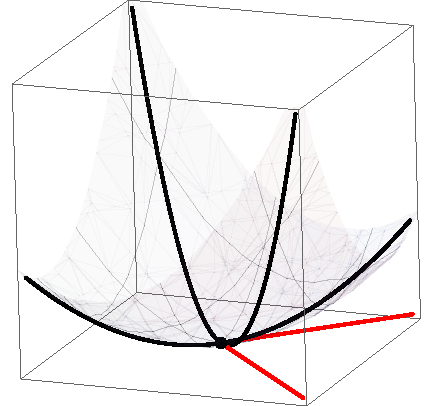
\includegraphics[width=2in]{03-Linear-Algebra-Applications/support/2nddertest1}
\hspace{.5in}
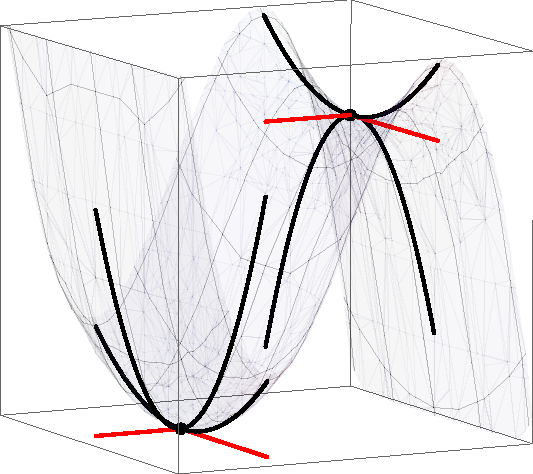
\includegraphics[width=2in]{03-Linear-Algebra-Applications/support/2nddertest2}
\end{center}
\caption{The eigenvectors of the second derivative tell you the directions in which the 2nd derivative is largest and smallest. At each critical point, two eigenvectors are drawn as well as a parabola whose second derivative (the eigenvalue) matches the second derivative of the surface in the corresponding eigenvector direction.}
\label{2ndder}
\end{figure}
%}}


\begin{example}
For the function {$f(x,y)=x^3-3x+y^2-4y$}, the gradient is $Df = \begin{bmatrix}3x^2-3&2y-4 \end{bmatrix}$, which is zero at $x=1,y=2$ or $x=-1,y=2$. Hence there are two critical points, so we have to find two sets of eigenvalues. The Hessian is $D^2f = \begin{bmatrix}6x&0 \\0&2\end{bmatrix}$. When $x=-1,y=2$, the eigenvalues of $\begin{bmatrix}-6&0 \\0&2\end{bmatrix}$ are $\lambda=-6,2$. Since one is positive and one is negative, there is a saddle point at $(-1,2)$. When $x=1,y=2$, the eigenvalues of $\begin{bmatrix}6&0 \\0&2\end{bmatrix}$ are $\lambda=6,2$. Since both are positive, there is a minimum at $(-1,2)$ (as in every direction the function is concave upwards).

Again the eigenvectors help us understand how the function behaves, as illustrated in figure \ref{2ndder}.  At (1,2) we have an eigenvector (1,0) corresponding to 6, and (0,1) corresponding to 2. In both eigenvector directions the function is concave upwards, but opens more stepply in the (1,0) direction as 6 is bigger than 2.  At (-1,2) the we have an eigenvector (1,0) corresponding to -6, and (0,1) corresponding to 2. The functions opens stepply downwards in the (1,0) direction, and upwards in the (0,1) direction. 
\end{example}










\newgeometry{left=1in,right=1in,top=1in,bottom=1in}

\section{Preparation}

This chapter covers the following ideas. When you create your lesson plan, it should contain examples which illustrate these key ideas. Before you take the quiz on this unit, meet with another student out of class and teach each other from the examples on your lesson plan. 

\begin{enumerate}

\item Find the currents in electrical systems involving batteries and resistors, using both Gaussian elimination and Cramer's rule.
\item Find interpolating polynomials. Use the transpose and inverse of a matrix to solve the least squares regression problem of fitting a line to a set of data.
\item Find the partial fraction decomposition of a rational function. Utilize this decomposition to integrate rational functions.
\item Describe a Markov process. Explain how an eigenvector of the eigenvalue $\lambda=1$ is related to the limit of powers of the transition matrix.
\item Explain how to generalize the derivative to a matrix. Use this generalization to locate optimal values of the function using the second derivative test. Explain the role  of eigenvalues and eigenvectors in the second derivative test.
\end{enumerate}


Here are the preparation problems for this unit. Please make sure you come to class having completed your problem, and able to explain to others how to do it.  We will often be doing problems very similar to the prep problems in class, and your preparation will help you contribute to your group. As time permits, I will post handwritten solutions to these problems on I-Learn. Please check there if you are struggling with your prep problem. 



\begin{center}
\begin{tabular}{ll|l}
\multicolumn{2}{c}{Preparation Problems (\href{http://ilearn.byui.edu/bbcswebdav/institution/Physical\_Sci\_Eng/Mathematics/Personal\%20Folders/WoodruffB/316/03-Linear-Algebra-Applications-Preparation-Solutions.pdf}{click for solutions})}
&
\href{http://www.youtube.com/user/bmwoodruff#grid/user/26D7C9E45A54794F}{Webcasts on YouTube - click here} 
%(
%\href{http://ilearn.byui.edu/bbcswebdav/institution/Physical\_Sci\_Eng/Mathematics/Personal\%20Folders/WoodruffB/341/2-Applications-videos.pdf}{pdf copy}
%)
\\
\hline\hline
Day 1&
1a, 1b, 2a, 3b
&
%\href{http://ilearn.byui.edu/bbcswebdav/institution/Physical\_Sci\_Eng/Mathematics/Personal\%20Folders/WoodruffB/341/2-Applications-video-01.wmv}{1},
%\href{http://ilearn.byui.edu/bbcswebdav/institution/Physical\_Sci\_Eng/Mathematics/Personal\%20Folders/WoodruffB/341/2-Applications-video-02.wmv}{2},
%\href{http://ilearn.byui.edu/bbcswebdav/institution/Physical\_Sci\_Eng/Mathematics/Personal\%20Folders/WoodruffB/341/2-Applications-video-03.wmv}{3}
\\ \hline
Day 2&
3f, 4c, 4d, 5b
&
%\href{http://ilearn.byui.edu/bbcswebdav/institution/Physical\_Sci\_Eng/Mathematics/Personal\%20Folders/WoodruffB/341/2-Applications-video-04.wmv}{4},
%\href{http://ilearn.byui.edu/bbcswebdav/institution/Physical\_Sci\_Eng/Mathematics/Personal\%20Folders/WoodruffB/341/2-Applications-video-05.wmv}{5},
%\href{http://ilearn.byui.edu/bbcswebdav/institution/Physical\_Sci\_Eng/Mathematics/Personal\%20Folders/WoodruffB/341/2-Applications-video-06.wmv}{6}
\\ \hline
Day 3&
6a, 6b, 7d, 7g 
&
%\href{http://ilearn.byui.edu/bbcswebdav/institution/Physical\_Sci\_Eng/Mathematics/Personal\%20Folders/WoodruffB/341/2-Applications-video-07.wmv}{7},
%\href{http://ilearn.byui.edu/bbcswebdav/institution/Physical\_Sci\_Eng/Mathematics/Personal\%20Folders/WoodruffB/341/2-Applications-video-08.wmv}{8},
%\href{http://ilearn.byui.edu/bbcswebdav/institution/Physical\_Sci\_Eng/Mathematics/Personal\%20Folders/WoodruffB/341/2-Applications-video-09.wmv}{9},
%\href{http://ilearn.byui.edu/bbcswebdav/institution/Physical\_Sci\_Eng/Mathematics/Personal\%20Folders/WoodruffB/341/2-Applications-video-10.wmv}{10},
%\href{http://ilearn.byui.edu/bbcswebdav/institution/Physical\_Sci\_Eng/Mathematics/Personal\%20Folders/WoodruffB/341/2-Applications-video-11.wmv}{11}
\\ \hline
Day 4&
Lesson Plan,
Quiz&
\\ \hline
\end{tabular}
\end{center}

	The problems listed below are found in this book. 
\begin{center}
\begin{tabular}{|l|l|l|l|l|}
\hline
Concept&Suggestions&Relevant Problems\\ \hline
Kirchoff's Laws&&1\\ \hline
Cramer's Rule&&2\\ \hline
Interpolating Polynomials&&3\\ \hline
Least Square Regression&&4\\ \hline
Partial Fraction Decomposition&&5\\ \hline
Markov Process&&6\\ \hline
2nd Derivative Test&&7\\ \hline
\end{tabular}
\end{center}

\section{Problems}

\begin{enumerate}
\item Consider the following electrical systems. Use the given values to find the current in each wire.

\centerline{\renewcommand{\myscale}{.3}
\begin{tikzpicture}[scale=\myscale,inner sep=1pt]
%\draw[help lines,step=1cm] (0,0) grid (12,6);

%Source - like a battery
\node[label=right:$E$] at (0,3)
{{\begin{tikzpicture}[scale=\myscale]
%	\useasboundingbox (-.5,-3) rectangle (.5,3);
	\draw (0,0) circle (1cm);
	\draw (.3,.5) -- (-.3,.5);
	\draw (0,.2) -- (0,.8);
	\draw (.3,-.5) -- (-.3,-.5);
	\draw (0,1) -- (0,3);
	\draw (0,-1) -- (0,-3);
	\end{tikzpicture}
}};

%Resistor
\node[label=right:$R_2$] at (6,3) 
{{\begin{tikzpicture}[scale=\myscale]
%	\useasboundingbox (0,-3) rectangle (0,3);
	\draw (0,-3) -- ++(0,1.8) -- ++(.5,.2) 
		-- ++(-1,.4) -- ++(1,.4)
		-- ++(-1,.4) -- ++(1,.4)
		-- ++(-1,.4) -- ++(.5,.2)
		-- ++(0,1.8) ;
	\end{tikzpicture}
}};

%Resistor
\node[label=above:$R_1$] at (3,0) 
{{\begin{tikzpicture}[scale=\myscale,rotate=90]
%	\useasboundingbox (0,-3) rectangle (0,3);
	\draw (0,-3) -- ++(0,1.8) -- ++(.5,.2) 
		-- ++(-1,.4) -- ++(1,.4)
		-- ++(-1,.4) -- ++(1,.4)
		-- ++(-1,.4) -- ++(.5,.2)
		-- ++(0,1.8) ;
	\end{tikzpicture}
}};

%Resistor
\node[label=right:$R_3$] at (12,3) 
{{\begin{tikzpicture}[scale=\myscale,rotate=0]
%	\useasboundingbox (0,-3) rectangle (0,3);
	\draw (0,-3) -- ++(0,1.8) -- ++(.5,.2) 
		-- ++(-1,.4) -- ++(1,.4)
		-- ++(-1,.4) -- ++(1,.4)
		-- ++(-1,.4) -- ++(.5,.2)
		-- ++(0,1.8) ;
	\end{tikzpicture}
}};

%Straight Path
\node at (3,6) 
{{\begin{tikzpicture}[scale=\myscale,rotate=90]
	\draw (0,-3) -- (0,3);
	\end{tikzpicture}
}};

%Straight Path
\node at (9,6) 
{{\begin{tikzpicture}[scale=\myscale,rotate=90]
	\draw (0,-3) -- (0,3);
	\end{tikzpicture}
}};

%Straight Path
\node at (9,0) 
{{\begin{tikzpicture}[scale=\myscale,rotate=90]
	\draw (0,-3) -- (0,3);
	\end{tikzpicture}
}};


%Arrow to represent Current
\node[label=above:$i_1$] at (3,6) 
{{\begin{tikzpicture}[scale=\myscale,rotate=-90]
%	\useasboundingbox (0,-.4) rectangle (0,.4);
	\filldraw (0,.4) -- (-.2,-.4) -- (0,-.3) -- (.2,-.4);
	\end{tikzpicture}
}};

%Arrow to represent Current
\node[label=right:$i_2$] at (6,5) 
{{\begin{tikzpicture}[scale=\myscale,rotate=180]
%	\useasboundingbox (0,-.4) rectangle (0,.4);
	\filldraw (0,.4) -- (-.2,-.4) -- (0,-.3) -- (.2,-.4);
	\end{tikzpicture}
}};

%Arrow to represent Current
\node[label=above:$i_3$] at (9,6) 
{{\begin{tikzpicture}[scale=\myscale,rotate=-90]
%	\useasboundingbox (0,-.4) rectangle (0,.4);
	\filldraw (0,.4) -- (-.2,-.4) -- (0,-.3) -- (.2,-.4);
	\end{tikzpicture}
}};

%Node
\node at (6,6) 
{{\begin{tikzpicture}[scale=\myscale,rotate=-90]
%	\useasboundingbox (0,-.4) rectangle (0,.4);
	\filldraw (0,0) circle (.15cm);
	\end{tikzpicture}
}};

%Node
\node at (6,0) 
{{\begin{tikzpicture}[scale=\myscale,rotate=-90]
%	\useasboundingbox (0,-.4) rectangle (0,.4);
	\filldraw (0,0) circle (.15cm);
	\end{tikzpicture}
}};

\end{tikzpicture}

\renewcommand{\myscale}{.3}
\begin{tikzpicture}[scale=\myscale,inner sep=1pt]
%\draw[help lines,step=1cm] (0,0) grid (18,6);

%Source - like a battery
\node[label=right:$E$] at (0,3) 
{{\begin{tikzpicture}[scale=\myscale]
%	\useasboundingbox (-.5,-3) rectangle (.5,3);
	\draw (0,0) circle (1cm);
	\draw (.3,.5) -- (-.3,.5);
	\draw (0,.2) -- (0,.8);
	\draw (.3,-.5) -- (-.3,-.5);
	\draw (0,1) -- (0,3);
	\draw (0,-1) -- (0,-3);
	\end{tikzpicture}
}};

%Resistor
\node[label=right:$R_2$] at (6,3) 
{{\begin{tikzpicture}[scale=\myscale]
%	\useasboundingbox (0,-3) rectangle (0,3);
	\draw (0,-3) -- ++(0,1.8) -- ++(.5,.2) 
		-- ++(-1,.4) -- ++(1,.4)
		-- ++(-1,.4) -- ++(1,.4)
		-- ++(-1,.4) -- ++(.5,.2)
		-- ++(0,1.8) ;
	\end{tikzpicture}
}};

%Resistor
\node[label=above:$R_1$] at (3,0) 
{{\begin{tikzpicture}[scale=\myscale,rotate=90]
%	\useasboundingbox (0,-3) rectangle (0,3);
	\draw (0,-3) -- ++(0,1.8) -- ++(.5,.2) 
		-- ++(-1,.4) -- ++(1,.4)
		-- ++(-1,.4) -- ++(1,.4)
		-- ++(-1,.4) -- ++(.5,.2)
		-- ++(0,1.8) ;
	\end{tikzpicture}
}};

%Resistor
\node[label=above:$R_3$] at (9,6) 
{{\begin{tikzpicture}[scale=\myscale,rotate=90]
%	\useasboundingbox (0,-3) rectangle (0,3);
	\draw (0,-3) -- ++(0,1.8) -- ++(.5,.2) 
		-- ++(-1,.4) -- ++(1,.4)
		-- ++(-1,.4) -- ++(1,.4)
		-- ++(-1,.4) -- ++(.5,.2)
		-- ++(0,1.8) ;
	\end{tikzpicture}
}};

%Resistor
\node[label=right:$R_4$] at (12,3) 
{{\begin{tikzpicture}[scale=\myscale,rotate=0]
%	\useasboundingbox (0,-3) rectangle (0,3);
	\draw (0,-3) -- ++(0,1.8) -- ++(.5,.2) 
		-- ++(-1,.4) -- ++(1,.4)
		-- ++(-1,.4) -- ++(1,.4)
		-- ++(-1,.4) -- ++(.5,.2)
		-- ++(0,1.8) ;
	\end{tikzpicture}
}};

%Resistor
\node[label=right:$R_5$] at (18,3) 
{{\begin{tikzpicture}[scale=\myscale,rotate=0]
%	\useasboundingbox (0,-3) rectangle (0,3);
	\draw (0,-3) -- ++(0,1.8) -- ++(.5,.2) 
		-- ++(-1,.4) -- ++(1,.4)
		-- ++(-1,.4) -- ++(1,.4)
		-- ++(-1,.4) -- ++(.5,.2)
		-- ++(0,1.8) ;
	\end{tikzpicture}
}};

%Resistor
\node[label=above:$R_6$] at (9,0) 
{{\begin{tikzpicture}[scale=\myscale,rotate=90]
%	\useasboundingbox (0,-3) rectangle (0,3);
	\draw (0,-3) -- ++(0,1.8) -- ++(.5,.2) 
		-- ++(-1,.4) -- ++(1,.4)
		-- ++(-1,.4) -- ++(1,.4)
		-- ++(-1,.4) -- ++(.5,.2)
		-- ++(0,1.8) ;
	\end{tikzpicture}
}};









%Straight Path
\node at (3,6) 
{{\begin{tikzpicture}[scale=\myscale,rotate=90]
	\draw (0,-3) -- (0,3);
	\end{tikzpicture}
}};

%Straight Path
\node at (15,6) 
{{\begin{tikzpicture}[scale=\myscale,rotate=90]
	\draw (0,-3) -- (0,3);
	\end{tikzpicture}
}};

%Straight Path
\node at (15,0) 
{{\begin{tikzpicture}[scale=\myscale,rotate=90]
	\draw (0,-3) -- (0,3);
	\end{tikzpicture}
}};






%Arrow to represent Current
\node[label=above:$i_1$] at (3,6) 
{{\begin{tikzpicture}[scale=\myscale,rotate=-90]
%	\useasboundingbox (0,-.4) rectangle (0,.4);
	\filldraw (0,.4) -- (-.2,-.4) -- (0,-.3) -- (.2,-.4);
	\end{tikzpicture}
}};

%Arrow to represent Current
\node[label=right:$i_2$] at (6,5) 
{{\begin{tikzpicture}[scale=\myscale,rotate=180]
%	\useasboundingbox (0,-.4) rectangle (0,.4);
	\filldraw (0,.4) -- (-.2,-.4) -- (0,-.3) -- (.2,-.4);
	\end{tikzpicture}
}};

%Arrow to represent Current
\node[label=above:$i_3$] at (7,6) 
{{\begin{tikzpicture}[scale=\myscale,rotate=-90]
%	\useasboundingbox (0,-.4) rectangle (0,.4);
	\filldraw (0,.4) -- (-.2,-.4) -- (0,-.3) -- (.2,-.4);
	\end{tikzpicture}
}};

%Arrow to represent Current
\node[label=right:$i_4$] at (12,5) 
{{\begin{tikzpicture}[scale=\myscale,rotate=180]
%	\useasboundingbox (0,-.4) rectangle (0,.4);
	\filldraw (0,.4) -- (-.2,-.4) -- (0,-.3) -- (.2,-.4);
	\end{tikzpicture}
}};

%Arrow to represent Current
\node[label=above:$i_5$] at (15,6) 
{{\begin{tikzpicture}[scale=\myscale,rotate=-90]
%	\useasboundingbox (0,-.4) rectangle (0,.4);
	\filldraw (0,.4) -- (-.2,-.4) -- (0,-.3) -- (.2,-.4);
	\end{tikzpicture}
}};

%Arrow to represent Current
\node[label=above:$i_6$] at (11,0) 
{{\begin{tikzpicture}[scale=\myscale,rotate=90]
%	\useasboundingbox (0,-.4) rectangle (0,.4);
	\filldraw (0,.4) -- (-.2,-.4) -- (0,-.3) -- (.2,-.4);
	\end{tikzpicture}
}};








%Node
\node at (6,6) 
{{\begin{tikzpicture}[scale=\myscale,rotate=-90]
%	\useasboundingbox (0,-.4) rectangle (0,.4);
	\filldraw (0,0) circle (.15cm);
	\end{tikzpicture}
}};

%Node
\node at (6,0) 
{{\begin{tikzpicture}[scale=\myscale,rotate=-90]
%	\useasboundingbox (0,-.4) rectangle (0,.4);
	\filldraw (0,0) circle (.15cm);
	\end{tikzpicture}
}};

%Node
\node at (12,0) 
{{\begin{tikzpicture}[scale=\myscale,rotate=-90]
%	\useasboundingbox (0,-.4) rectangle (0,.4);
	\filldraw (0,0) circle (.15cm);
	\end{tikzpicture}
}};

%Node
\node at (12,6) 
{{\begin{tikzpicture}[scale=\myscale,rotate=-90]
%	\useasboundingbox (0,-.4) rectangle (0,.4);
	\filldraw (0,0) circle (.15cm);
	\end{tikzpicture}
}};

\end{tikzpicture}
}
\begin{multicols}{2}
\begin{enumerate}

\item $E=12, R_1=2,R_2=2, R_3=2$.
\item $E=12, R_1=2,R_2=3, R_3=3$.
\item $E=12, R_1=2,R_2=3, R_3=6$.
\item $E=12, R_1=1,R_2=2, R_3=2$.
\item $E=9, R_1=3,R_2=1, R_3=2$.
\item $E=6, R_1=1,R_2=1, R_3=2$.
\end{enumerate}
\end{multicols}


\begin{enumerate} \setcounter{enumii}{6}
\item $E=12$, $R_1=1$, $R_2=1$, $R_3=1$, $R_4=1$, $R_5=1$, $R_6=1$
\item $E=12$, $R_1=2$, $R_2=1$, $R_3=3$, $R_4=4$, $R_5=2$, $R_6=3$
\end{enumerate}


\item Use Cramer's rule to find solutions to the following linear systems. If Cramer's rule fails, explain why.

\begin{enumerate}
\begin{multicols}{2}
\item $2x+3y=0, x-2y=1$
\item $x+y=2, x-y=3$
\item $3x+y=6, x+3y=2$
\item $2x+y=1, 4x+2y=2$
\item $x+y=0, 2x-y+z=1, x+z=0$
\item $x+2y=3, x-y+z=0, x+3y+z=1$
\item $y+2z=1, x-z=3, 2x+y=1$
\end{multicols}
\end{enumerate}





\item In each of the following scenarios, find a polynomial of least degree which passes through the given points. Then plot the points and the polynomial.
\begin{enumerate}
\begin{multicols}{2}
\item $(1,2),(3,3)$ 			
\item $(0,1),(2,3),(-1,4)$  
\item $(1,1),(2,2),(-1,5)$   
\item $(1,2),(3,3),(5,6)$ 			
\item $(1,2),(3,3),(5,5)$ 
\item $(0,1),(1,3),(-1,4),(2,4)$ 
\end{multicols}
\end{enumerate}



\item For each set of data points, find an equation of the least squares regression line. Plot the points and the line on the same axes.

\begin{enumerate}
\begin{multicols}{2}
\item $(0,0),(1,3),(1,2)$
\item $(1,1),(2,1),(3,2)$
\item $(1,2),(3,0),(5,1)$
\item $(0,0),(1,3),(1,2),(4,5)$
\item $(0,0),(1,3),(1,2),(4,-5)$
\item $(-1,2),(1,3),(2,5),(3,3)$
\item Challenge: Find an equation of the least squares regression parabola $y=ax^2+bx+c$ which passes through the points $(0,0),(1,3),(1,2),(4,5)$. [Hint, you will need a 4 by 3 matrix for $A$ instead of an $n$ by $2$. Use the transpose to reduce the size of the matrix to a 3 by 3 matrix, and then solve.]
\end{multicols}
\end{enumerate}




\item Compute each integral by finding a partial fraction decomposition. 
\begin{enumerate}
\begin{multicols}{2}
\item $\ds\int\frac{1}{(x-3)(x+2)}dx $%, \frac{A}{x-3}+\frac{B}{x+2}$         
\item $\ds\int\frac{2x+3}{(x-3)(x+2)}dx$%, \frac{A}{x-3}+\frac{B}{x+2}$ 
\item $\ds\int\frac{x}{(x+1)(x-2)}dx$%,  \frac{A}{x+1}+\frac{B}{x-2}$  
\item $\ds\int\frac{x^2+2}{x^2(x-2)}dx$%, \frac{A}{x}+\frac{B}{x^2}+\frac{C}{x-2}$ 
\item $\ds\int\frac{1}{(x^2+1)(x-2)}dx$%, \frac{Ax+B}{x^2+1}+\frac{C}{x-2}$
\item $\ds\int\frac{x+1}{(x^2+1)x^2}dx$%, \frac{Ax+B}{x^2+1}+\frac{C}{x}+\frac{D}{x^2}$  
\end{multicols}
\end{enumerate}








\item Markov Process - In each scenario, write the transition matrix. If an initial state is given, then find the next two states. Finish by finding a steady state solution and use it to answer the question at the end.
%\begin{multicols}{2}
\begin{enumerate}

\item In a certain town, there are 3 types of land zones: residential, commercial, and industrial. The city has been undergoing growth recently, and the city has noticed the following trends.  Every 5 years, 10\% of the older residential land gets rezoned as commercial land, while 5\% gets rezoned as industrial.  The other 85\% remains residential.  For commercial land, 70\% remains commercial, while 10\% becomes residential and 20\% becomes industrial. For industrial land, 60\% remains industrial, while 25\% becomes commercial and 15\% becomes residential. Currently the percent of land in each zone is 40\% residential, 30\% commercial, and 30\% industrial. What will the percent distribution be in 5 years? In 10 years?  If this trend continues indefinitely, what percent of the land will eventually be residential?. 
\item Suppose we own a car rental company which rents cars in Idaho Falls and Rexburg. The last few weeks have shown a weekly trend that 60\% of the cars rented in Rexburg will remain in Rexburg (the other 40\% end up in IF), whereas 80\% of the cars rented in Idaho Falls will remain in Idaho Falls. If there are currently 60 cars in Rexburg and 140 cars in IF, how many will be in each city next week?  In two weeks? In three weeks? If this trend continues indefinitely, about how many cars should you expect to find in Rexburg each week?
\item Repeat the previous problem if 40\% of the cars rented in Rexburg will remain in Rexburg (the other 60\% end up in IF), whereas 80\% of the cars rented in Idaho Falls will remain in Idaho Falls.
\item Repeat the previous problem if 70\% of the cars rented in Rexburg will remain in Rexburg (the other 30\% end up in IF), whereas 80\% of the cars rented in Idaho Falls will remain in Idaho Falls.
\item A school cafeteria regularly offers 3 types of meals to its students. One of the meals is always a pizza/salad combo, One is always hamburgers and fries, and one is a daily special which changes daily. In an attempt to understand student preferences, the school discovered the following information. If a student has a hamburger one day, then there is a 30\% chance they will try the daily special the next day, and a 40\% percent chance they will have the salad bar.  If they have the salad bar, then there is a 30\% chance they'll switch to the daily special, and a 40\% chance they'll switch to the hamburger.  If the have the daily special, then there is a 50\% chance they'll get the daily special the next day, a 20\% chance they'll switch to pizza, and a 30\% chance they'll switch to hamburger.  If this trend continues, what percent of the students will eat each type of meal? 

[While this problem is highly rigged, there is a branch of applied mathematics which is studied by financial analysts call stochastic processes which models such a scenario. This modeling process can help predict how a new restaurant will perform in a city, sometimes predict stock market fluctuations, and more. The study of stochastic processes begins with a Markov process and then introduces statistics and probability to help predict what happens when trends change.]
\end{enumerate}
%\end{multicols}





\item For each function, find the location of all critical points. Then use the second derivative test to determine if each critical point corresponds to a maximum, minimum, or saddle point. Graph the function in 3D to verify your results, and locate the eigenvectors and eigenvalues in the picture.
\begin{multicols}{2}
\begin{enumerate}
\item $f(x,y) = x^2+xy+y^2$
\item $f(x,y) = x^2+4xy+y^2$
\item $f(x,y) = x^2+2xy+y^2$
\item $f(x,y) = x^2-4x+y^2+2y+1$
\item $f(x,y) = x^2-2x+xy+y^2$
\item $f(x,y) = x^2+xy+3y^2$
\item $f(x,y) = x^3-3x+y^2-2y$ (2 critical points)
\item $f(x,y) = x^3-3x+y^3-3y^2$ (4 critical points)
\end{enumerate}
\end{multicols}












\end{enumerate}








\section{Solutions}
{
\begin{multicols}{2}


\newpage
\small
Remember that the Technology introduction has a step-by-step guide for solving many of these problems.
\begin{enumerate}

\item Kirchoff's Laws

 $\begin{bmatrix}[lll|l]
 1 & -1 & -1 & 0 \\
 R_1 & R_2 & 0 & E \\
 0 & -R_2 & R_3 & 0
\end{bmatrix}$

\begin{enumerate}
\item $(4,2,2)$
\item $(24/7,12/7,12/7)$
\item $(3,2,1)$
\item $(6,3,3)$
\item $(27/11,18/11,9/11)$
\item $(18/5,12/5,6/5)$

$\begin{bmatrix}[llllll|l]
 1 & -1 & -1 & 0 & 0 & 0 & 0 \\
 0 & 0 & 1 & -1 & -1 & 0 & 0 \\
 0 & 0 & 0 & 1 & 1 & -1 & 0 \\
 R_1 & R_2 & 0 & 0 & 0 & 0 & E \\
 0 & -R_2 & R_3 & R_4 & 0 & R_6 & 0 \\
 0 & 0 & 0 & -R_4 & R_5 & 0 & 0
\end{bmatrix}$

\item $\left\{7, 5, 2, 1, 1, 2\right\}$

\item $\left\{\frac{25}{6},\frac{11}{3},\frac{1}{2},\frac{1}{6},\frac{1}{3},\frac{1}{2}\right\}$
\end{enumerate}


\item Cramer's rule
\begin{enumerate}
\item $\left\{\frac{3}{7},-\frac{2}{7}\right\}$
\item $\left\{\frac{5}{2},-\frac{1}{2}\right\}$
\item $\{2,0\}$
\item Fails. The determinant of the coefficient matrix is zero.
\item $\left\{\frac{1}{2},-\frac{1}{2},-\frac{1}{2}\right\}$
\item $\left\{\frac{5}{2},\frac{1}{4},-\frac{9}{4}\right\}$
\item Fails. The determinant of the coefficient matrix is zero.
\end{enumerate}





\item Interpolating Polynomials
\begin{enumerate}
\item $1/2 x + 3/2$
\item $(4/3)x^2-(5/3)x+1$
\item $x^2-2x+2$
\item $(1/4)x^2-(1/2)x+9/4$
\item $(1/8)x^2+15/8$
\item $-x^3+(5/2)x^2+(1/2)x+1$
\end{enumerate}


\item Regression (Make the plots using technology)

\begin{enumerate}
\item $y=\frac{5 x}{2}$
\item $y=\frac{x}{2}+\frac{1}{3}$
\item $y=\frac{7}{4}-\frac{x}{4}$
\item $y=\frac{10 x}{9}+\frac{5}{6}$
\item $y=\frac{5}{2}-\frac{5 x}{3}$
\item $y=\frac{3 x}{7}+\frac{19}{7}$
\item 
$
A=
\begin{bmatrix} 
 0 & 0 & 1 \\
 1 & 1 & 1 \\
 1 & 1 & 1 \\
 16 & 4 & 1
\end{bmatrix},
B=
\begin{bmatrix} 
 0 \\
 3 \\
 2 \\
 5
\end{bmatrix},
A^T A=
\begin{bmatrix} 
 258 & 66 & 18 \\
 66 & 18 & 6 \\
 18 & 6 & 4
\end{bmatrix},
A^T B=
\begin{bmatrix} 
 85 \\
 25 \\
 10
\end{bmatrix}$,

$y=-\frac{5}{12}x^2+\frac{35}{12}x+0
$
\end{enumerate}






\item Partial Fractions
\begin{enumerate}
\item $-1/5\,\ln  \left( x+2 \right) +1/5\,\ln  \left( x-3 \right)$
\item $1/5\,\ln  \left( x+2 \right) +9/5\,\ln  \left( x-3 \right) $
\item $1/3\,\ln  \left( x+1 \right) +2/3\,\ln  \left( x-2 \right) $
\item ${x}^{-1}+3/2\,\ln  \left( x-2 \right) -1/2\,\ln  \left( x \right)$
\item $-\frac{1}{10}\ln  \left( {x}^{2}+1 \right) -\frac{2}{5}\arctan \left( x \right) +\frac{1}{5}\ln  \left( x-2 \right) $
\item $-{x}^{-1}-1/2\,\ln  \left( {x}^{2}+1 \right) -\arctan \left( x
 \right) +\ln  \left( x \right)
$
\end{enumerate}








\item Markov Process

\begin{enumerate}
\item Transition matrix 
$\begin{bmatrix}
 0.85 & 0.1 & 0.15 \\
 0.1 & 0.7 & 0.25 \\
 0.05 & 0.2 & 0.6
\end{bmatrix}$,
5 years  (41.5,32.5,26), 
10 years: (42.425,33.4,24.175),
Steady state: $[4,3,2]^T$ so 4/9 or 44.4\% will be residential. 

\item
Transition matrix 
$\begin{bmatrix}
 {3}/{5} & {1}/{5} \\
 {2}/{5} & {4}/{5}
\end{bmatrix}$,
1 week  (64,136), 
2 week: (65.6,134.4),
3 week: (66.24,133.76),
Steady state: $[1,2]^T$ so 1/3 (33.3\%) will be in Rexburg. This means 66 or 67 cars will be in Rexburg. 
 
\item 
Transition matrix 
$\begin{bmatrix}
 {2}/{5} & {1}/{5} \\
 {3}/{5} & {4}/{5}
\end{bmatrix}$,
1 week  (52,148), 
2 week: (50.4,149.6),
3 week: (50.08,149.92),
Steady state: $[1,3]^T$ so 1/4 or 25\% will be in Rexburg. This means 50 cars will be in Rexburg. 

\item 
Transition matrix 
$\begin{bmatrix}
 {7}/{10} & {1}/{5} \\
 {3}/{10} & {4}/{5}
\end{bmatrix}$,
1 week  (70,130), 
2 week: (75,125),
3 week: (77.5,122.5),
Steady state: $[2,3]^T$ so 2/5 or 40\% will be in Rexburg. This means 80 cars will be in Rexburg. 

\item My order is hamburger, pizza/salad, special (your order may vary which means your matrix will be a little different, but the eigenvector will still have the same ratios).
Transition matrix 
$\begin{bmatrix}
 {3}/{10} & {2}/{5} & {3}/{10} \\
 {2}/{5} & {3}/{10} & {1}/{5} \\
 {3}/{10} & {3}/{10} & {1}/{2}
\end{bmatrix}$,
Steady state: $[29,26,33]^T$ or $[29/88,26/88,33/88]^T$ so Hamburger - 32.9545\%, Pizza/Salad - 29.5455\%, Special - 37.5\%. 

\end{enumerate}






\item Second Derivative Test
\begin{enumerate}
\item At $(0,0)$ eigenvalues are $3,1$ (both positive so min) with eigenvectors $[1,1]^T,[-1,1]^T$.
\item At $(0,0)$ eigenvalues are $6,-2$ (saddle point) with eigenvectors $[1,1]^T,[-1,1]^T$.
\item At $(0,0)$ eigenvalues are $4,0$ (test fails) with eigenvectors $[1,1]^T,[-1,1]^T$.
\item At $(2,-1)$ eigenvalues are $2,2$ (both positive so min) with eigenvectors $[1,0]^T,[0,1]^T$.
\item At $(4/3,-2/3)$ eigenvalues are $3,1$ (both positive so min) with eigenvectors $[1,1]^T,[-1,1]^T$.
\item At $(0,0)$ eigenvalues are $6.23607,1.76393$ (both positive so min) with eigenvectors $[.236,1]^T,[-4.236,1]^T$.
\item 
At $(-1,1)$ eigenvalues are $-6,2$ (saddle) with eigenvectors $[1,0]^T,[0,1]^T$.
At $(1,1)$ eigenvalues are $6,2$ (both positive so min) with eigenvectors $[1,0]^T,[0,1]^T$.
\item 
At $(-1,0)$ eigenvalues are $-6,-6$ (both negative so max) with eigenvectors $[1,0]^T,[0,1]^T$.
At $(-1,2)$ eigenvalues are $-6,6$ (saddle) with eigenvectors $[1,0]^T,[0,1]^T$.
At $(1,0)$ eigenvalues are $6,-6$ (saddle) with eigenvectors $[1,0]^T,[0,1]^T$.
At $(1,2)$ eigenvalues are $6,6$ (both positive so min) with eigenvectors $[1,0]^T,[0,1]^T$.

\end{enumerate}




























	
\end{enumerate}


\end{multicols}
}





\restoregeometry



\chapter{First Order ODEs}

\noindent  
This chapter covers the following ideas. When you create your lesson plan, it should contain examples which illustrate these key ideas. Before you take the quiz on this unit, meet with another student out of class and teach each other from the examples on your lesson plan. 



\begin{enumerate}
\item Be able to interpret the basic vocabulary of differential equations. In particular, interpret the terms ordinary differential equation (ODE), initial value, initial value problem (IVP), general solution, and particular solution.
\item Use the three step modeling process (express, solve, and interpret) to analyze exponential growth and decay, Newton's law of cooling, mixing, and the logistics equation. 
\item Identify and solve separable ODES and exact differential forms. Use integrating factors and substitutions to solve additional ODEs.
\item Use Laplace transforms to solve first order ODEs.
\end{enumerate}




\section{Basic Concepts and Vocabulary}
A differential equation is an equation which involves derivatives (of any order) of some function.  For example, the equation $y^{\prime\prime}+xy^\prime+\sin(xy)=xy^2$ is a differential equation. An \textbf{ordinary differential equation (ODE)} is a differential equation involving a function $y(x)$ whose domain is one dimensional. A solution to an ODE on an interval $J=(a,b)$ is a function $y(x)$ defined on the interval $J$ which satisfies the ODE.  To verify that a function is a solution to an ODE, calculate derivatives and put them in the ODE. If the resulting equation is an identity for all $x\in J$, then you have a solution. The order of an ODE is the largest order derivative that appears in the ODE. 

Typically a solution to an ODE involves an arbitrary constant $C$. There is often an entire family of curves which satisfy a differential equation, and the constant $C$ just tells us which curve to pick. A \textbf{general solution} of an ODE is all possible solutions of the ODE.  A \textbf{particular solution} is one of infinitely many solutions of an ODE. Often an ODE comes with an \textbf{initial condition} $y(x_0)=y_0$ for some values $x_0$ and $y_0$. We can use these initial conditions to find a particular solution of the ODE. An ODE, together with an initial condition, is called an \textbf{initial value problem (IVP)}.  

\begin{example}
The ODE $y^\prime = ky$ has the general solution $y=ce^{kx}$ for $x\in(-\infty,\infty)$. We check that this is a solution by calculating $\frac{d}{dx}ce^{kx} = kce^{kx}=ky$. This is a first order ODE because only the first derivative and no higher derivatives appear in the ODE.  If the initial condition $y(0)=3$ were also in the problem, then the particular solution to this IVP is found by solving for $c$ in the equation $3=ce^{k0}$.  This simplifies to $c=3$, so $y(x) = 3e^{kx}$ is the solution to the IVP  $y^\prime = ky$, $y(0)=3$.
\end{example}

%\subsection{Direction Fields}
%A first order ODE of the form $y^\prime=f(x,y)$ can be used to describe a vector field which represents the slope of $y$ at each point in the plane. Since $y^\prime$ is the slope of $y$, the graph of the vector field $\vec F = \left<1,y^\prime\right>$ gives a picture of how $y$ changes depending on which point $(x,y)$ in the plane you are at.  This graph is called a direction field, and it is used to visually see what a solution should look like.  Solutions to a first order ODE will follow the direction vectors in the direction field.  Some ODEs are so complex that no known method of solving them is available, and so direction fields give a way of visually approximating a solution.  Some examples follow. The first two examples include several particular solutions of the ODE for different initial conditions.
%
%
%\newcommand{\mywidth}{1.3in}
%\begin{center}
%\begin{tabular}{cccc}
%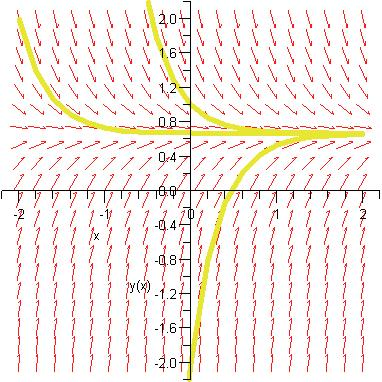
\includegraphics[width=\mywidth]{Basic-ODEs/dirfield-1}&
%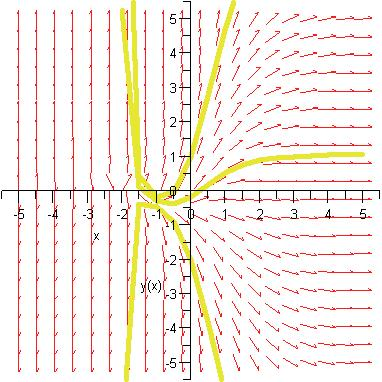
\includegraphics[width=\mywidth]{Basic-ODEs/dirfield-2}&
%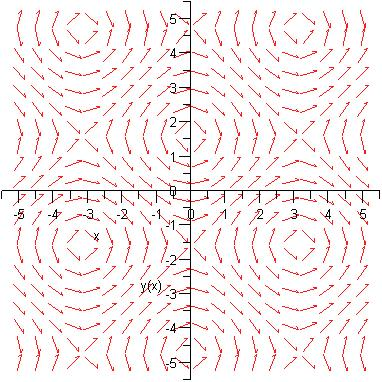
\includegraphics[width=\mywidth]{Basic-ODEs/dirfield-3}&
%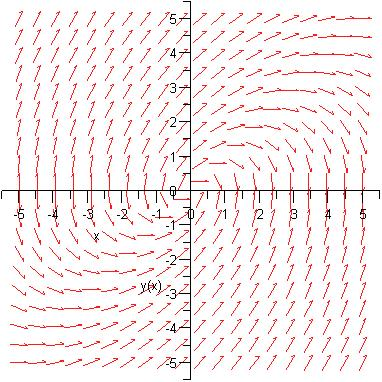
\includegraphics[width=\mywidth]{Basic-ODEs/dirfield-4}
%\\
%$y^\prime+3y = 2$&
%$e^{x}\frac{dy}{dx}= 2y+\cos(x)$ &
%$\cos(y)y^\prime= \sin(x)$ &
%$(x-y)dx+ydy=0$
%\end{tabular}
%\end{center}
%
% 




\section{Modeling Basics}
Many quantities in the world can be described in terms of rates of change. Differential equations arise in any physical model where rates of change are part of the model. Modeling requires that we (1) express quantities in terms of mathematical equations, (2) solve those equations, and (3) interpret the results in the context of our original problem.  The first and third steps require human intervention, while the second step can often be solved with the aid of technology. We will start by looking at three models: exponential growth and decay, Newton's law of cooling,  and mixing. I will illustrate steps (1) and (3) first, and then in the next section we will focus on methods of solving.


\subsection{Exponential Model}
Exponential growth and decay models radioactive decay, retirement investing, carbon dating, population growth, and more. The model is based on the principle that the rate of change of a quantity is directly proportional to the quantity itself.  The rate of decay of a radioactive isotope is proportional to the amount of the isotope that remains.  The rate of increase in a retirement investment is proportional to how much money is in the retirement investment. If you double an investment, then it should grow twice as quickly. We now follow the three steps.
\begin{enumerate}
	\item (Express) The derivative is proportional to the quantity itself can be expressed mathematically by the formula $y^\prime(x)=ky(x)$, where $k$ is some constant. 
	\item (Solve)  The general solution to this ODE is $y(x) = ce^{kx}$. (Solved in example~\ref{expsol})
	\item (Interpret) When $x=0$, we have $y=c$. This means that $c$ is the initial amount of a radioactive isotope, or the initial investment in a retirement portfolio.  The constant $k$ helps us determine how quickly an isotope decays ($k<0$), or how quickly an investment grows ($k>0$).  
\end{enumerate}





\subsection{Newton's Law of Cooling}
One version of Newton's law of cooling states that the rate of change of temperature $\frac{dT}{dt}$ of a body (which conducts heat well) is proportional to the difference between the current temperature $T(t)$ of the body and the temperature $T_A$ of the surrounding atmosphere (which is assumed to be constant).
\begin{enumerate}
	\item (Express) Newton's law of cooling can be expressed mathematically as $ \frac{dT}{dt} = k(T-T_A)$ for some constant $k$.  If $T>T_A$, then the temperature needs to drop, so we know $k<0$. If $T<T_A$, then the temperature needs to rise, so $k<0$ gives $k(T-T_A)>0$ as the product of two negatives. In all cases, the constant $k$ will hence be negative.
	\item (Solve)  The general solution to this ODE is $y = T_A+ce^{kt}$ (solved in Example~\ref{newtonsol}).
	\item (Interpret) When $t=0$, we have $T(0)=T_A+c$. This means that $c=T(0)-T_A$ is the initial difference in temperature.  Since $k$ is always negative, as $t\to\infty$ the temperature $T(t)$ approaches $T_A$, the temperature of the surrounding atmosphere.  
\end{enumerate}

\subsection{Mixing Model}
We will encounter mixing problems throughout the semester of the following type.  Suppose a 5000 gallon tank contains a solution of water which initially contains 200 lbs of salt. The tank has an inflow valve, and an outflow value.  Suppose 30 gallons of water (with 3 lbs of salt per gallon) are pumped into the tank each minute. The mixture is evenly spread throughout the entire tank by constant stirring.  At the same time, 30 gallons of the stirred mixture flow through the outflow valve each minute.  Find the amount of salt in the tank at time $t$.

%\begin{wrapfigure}{l}{0pt}
%	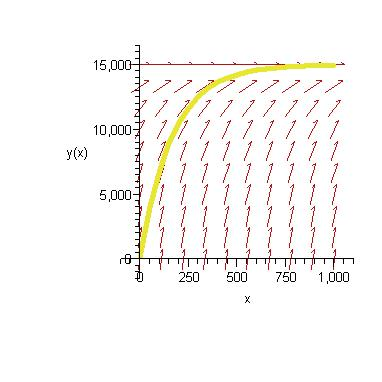
\includegraphics[width=1.5in]{Basic-ODEs/model-1}
%\end{wrapfigure}

\begin{enumerate}
	\item (Express) If we let $y(t)$ be the amount of salt in the tank at any time $t$, then $y^\prime=\text{(flow in)}-\text{(flow out)}$. The flow in is 
	$$\text{flow in }=\frac{30 \text{ gal}}{\text{min}}\bigg|\frac{3 \text{ lbs}}{\text{gal}} = \frac{90 \text{ lbs}}{\text{min}} \text{ of salt.}$$ 
The amount of salt lost per minute is proportional to the amount of salt in the tank. Since the tank holds 5000 gallons, and the outflow is 30 gal/min, we loose $\frac{30}{5000}$ of the water in the tank each minute.  Since the mixture is evenly stirred, this means that $\frac{30}{5000}$ of what currently is in the tank (which is $y$ lbs) should leave every minute.  So our flow out is\
	$$\text{flow out }=\frac{30 \frac{\text{gal}}{\text{min}}}{5000 \text{ gal}}\bigg|y \text{ lbs} = \frac{30}{5000}y \frac{\text{lbs}}{\text{min}} \text{ of salt.}$$ 
Hence $y^\prime = 90-\frac{30}{5000}y$. The initial condition is $y(0)=200$ lbs.
	\item (Solve) The general solution is $y(t) = 15000+c e^{(-3/500) t}$.  Using $y(0)=200$, we find $200=15000+c,$ or $c=-14800$.  So $y(t) = 15000-14800 e^{(-3/500) t}$.
	\item (Interpret) The salt content starts at 200 lbs and grows to a maximum of 15000 lbs as $t\to\infty$.  The quantity grows more rapidly at the beginning than at the end.
\end{enumerate}





\section{Basic Methods}
The modeling process often results in a differential equation. We will learn various methods of solving these differential equations. Software can solve the differential equations in this course,  however, the differential equations you may encounter in the future might not be solvable by any of the methods in this textbook or by software.  Understanding the ideas and processes which go into these methods will give you building blocks which you may need to creatively solve new differential equations.  

\subsection{Separable}
The most basic differential equation to solve is one in which you can ``separate'' the variables.  The idea is to rearrange the equation in the form $f(y)dy=g(x)dx$, where you separate the $x$ and $y$ terms so that they appear on different sides of the equation.  The solution is found by integrating each side.

\begin{example}[Exponential Model Solution] \label{expsol} Divide the differential equation $y^\prime = ky$ on both sides by $y$. Then multiply both sides by the differential $dx$ to obtain $\frac{1}{y}dy = k dx$. Integration on both sides yields $\ln|y| = kx+c$.  Exponentiating both sides gives $|y|=e^{kx+c}=e^{kx}e^c$. Now $e^c$ is a positive constant, so we rename that constant to be $c$ and obtain $|y|=ce^{kx}$ for $c>0$.  Removing the absolute values on $y$ allows $c$ to be any nonzero constant. If $c=0$, then the equation $y=0$ satisfies the differential equation $y^\prime = ky$, so we can let $c=0$ as well. This shows that a general solution to $y^\prime = ky$ is $y(x)=ce^{kx}$ for any constant $c$.
\end{example}

\begin{example}[Newton's Law of Cooling Solution] \label{newtonsol}The differential equation for Newton's law of cooling, $ \frac{dT}{dt} = k(T-T_A)$, is another separable ODE. Rearrange the equation as $\frac{1}{T-T_A}dT = kdt$.  Integration yields $\ln|T-T_A|=kt+c$.  Exponentiation gives $|T-T_A|=e^{kt+c}=e^{kt}e^c=ce^{kt}$.  Removing absolute values as before gives $T=T_A+ce^kt$ as a general solution. 
\end{example}

\subsection{Exact Differential Forms}
Recall that a vector field $\vec F=\left<M,N\right>$ is called a gradient field if there exists a function $f(x,y)$, called a potential for $F$, which satisfies $\nabla f = \vec F$. Recall also that $\vec F=\left<M,N\right>$ has a potential (under suitable conditions) if and only if $M_y=N_x$ (test for exactness). Similarly, a differential form $Mdx+Ndy$ is said to be exact if there exists a function $f(x,y)$ which satisfies $df=Df(x,y)\begin{bmatrix}dx\\ dy\end{bmatrix}= Mdx+Ndy$. If a first order differential equation can be written in the form $Mdx+Ndy=0$, and that differential form is exact, then a general solution to the ODE is $f(x,y)=c$ for any constant $c$, where $f$ is a potential for $\left<M,N\right>$. 
\marginpar{A general solution to $Mdx+Ndy=0$ is $f=c$ where $f$ is a potential for $\left<M,N\right>$ and $c$ is an arbitrary constant.}  
This is because the level curves of the potential ($f=c$) are orthogonal to the gradient of the potential, which is precisely what $\left<M,N\right>\cdot\left<dx,dy\right>=0$ means. 

\begin{example}
The differential equation $3xy^\prime = 2x-3y$ can be rewritten in the differential form $(3y-2x)dx+3xdy=0$. We calculate $M_y=\frac{\partial}{\partial y}(3y-2x) = 3$ and $N_x=\frac{\partial}{\partial x}(3x) = 3$. Since $M_y=N_x$, a potential exists. We integrate both terms and obtain  
$$\int M dx = 3xy-x^2 \quad\bigg|\quad \int N dy = 3xy.$$ Summing the integrals and ignoring duplicates, we obtain $f=3xy-x^2$ as a potential.  The general solution of $3xy^\prime = 2x-3y$ is $3xy-x^2=c$ for any constant $c$. We have written the solution implicitly (without solving explicitly for $y$). Solving for $y$ gives the explicit solution $y=\frac{c+x^2}{3x}$, however you may not always be able to solve for $y$.  
\end{example}

Notice that if a differential equation is separable $f(y)dy=g(x)dx$, then it represents an exact differential form, namely $-g(x)dx+f(y)dy=0$ has potential $-\int g(x)dx + \int f(y)dy$.  Every separable differential equation can be solved by considering exact differential forms. \marginpar{Solving an exact ODE is the BIG IDEA.} In fact, the goal of every method below is to rewrite the ODE so that it is an exact differential form, which means that finding a potential is the BIG IDEA of this unit.

\subsection{Integrating Factors (What to do if it isn't exact)}

Not every differential equation, when written in differential form $Mdx+Ndy=0$ is exact.  However, by multiplying both sides by an appropriate factor (called an integrating factor), often we can make the ODE exact. 

\begin{example}
The differential form $-kydx+dy=0$ (which models exponential growth) is not exact. However, if you multiply both sides by $e^{-kx}$, then the differential form $-ke^{-kx}ydx+e^{-kx}dy=0$ is exact with potential $f=ye^{-kx}$, and hence the solution is $ye^{-kx}=c$ or $y=ce^{kx}$ as before.  Alternatively, we could multiply both sides of $-kydx+dy=0$ by $\frac{1}{y}$. This gives the differential form $-kdx+\frac{1}{y}dy=0$, which is exact with potential $f=-kx+\ln|y|$. The general solution is thus $-kx+\ln|y|=c$ which becomes $\ln|y|=kx+c$ and simplifies to $y=ce^{kx}$ as before. In either case we multiplied a non exact differential form by a factor (called an integrating factor) to obtain an exact differential form.  
\end{example}

Essentially every method we look at for this unit can be solved by finding an appropriate integrating factor and then finding a potential to get the general solution. So how do we find an appropriate integrating factor? If a differential form $Mdx+Ndy$ is not exact, then we seek a function $F$ so that $FMdx+FNdy$ is exact.  To simplify our work, we will consider two cases: (1) $F$ is a function which depends on only $x$, or (2) $F$ is a function which depends on only $y$.  
\begin{enumerate}
	\item If $F=F(x)$, then for $FMdx+FNdy$ to be exact we must have $(FM)_y=(FN)_x$, which is equivalent to $FN_y = FM_x+F_xM$. Rearranging (separating $F$ from the other terms) gives $ \frac{1}{F}F_x = \frac{M_y-N_x}{N}$. Integrating both sides yields $ \ln|F| = \int\frac{M_y-N_x}{N}dx$.  Solving for $F$ gives $ F(x)=e^{\int\frac{M_y-N_x}{N}dx}$. The preceding formula will give us our integrating factor as long as  $ \frac{M_y-N_x}{N}$ depends only on $x$.
	\item If $F=F(y)$, then for $FMdx+FNdy$ to be exact we must have $(FM)_y=(FN)_x$, which is equivalent to $FM_y+F_yM = FN_x$. Rearranging gives $ \frac{1}{F}F_y = \frac{N_x-M_y}{M}$. Integrating both sides yields $ \ln|F| = \int\frac{N_x-M_y}{M}dx$, and solving for $F$ gives $ F(y)=e^{\int\frac{N_x-M_y}{M}dy}$. The preceding formula will give us our integrating factor as long as  $ \frac{N_x-M_y}{M}$ depends only on $y$.

\end{enumerate}
\begin{observation}
If  $\ds \frac{M_y-N_x}{N}$ depends on $x$, then $\ds e^{\int \frac{M_y-N_x}{N} dx}$ is an integrating factor. If $\ds\frac{N_x-M_y}{M}$ depends on $y$, then $\ds e^{\int \frac{N_x-M_y}{M} dy}$ is an integrating factor.
\end{observation}

\begin{example}
To solve the differential equation $(x+y)dx+3xdy=0$, we compute $M_y-N_x=1-3=-2$.  Division by $N$ gives $\frac{M_y-N_x}{N} = \frac{-2}{3x}$.  Hence $F=e^{\int -2/(3x) dx} = e^{-2/3 \ln(x)}=x^{-2/3}$. Then the differential form $(x^{1/3}+x^{-2/3}y)dx+3x^{1/3}dy=0$ has potential $\frac{3 x^{4/3}}{4}+3x^{1/3}y$.  So a general solution is $\frac{3 x^{4/3}}{4}+3x^{1/3}y=c$ or $y=\frac{c-\frac{3 x^{4/3}}{4}}{3x^{1/3}} $.
\end{example}

\subsection{Linear ODEs - a common special form}

A linear ODE is an ODE of the form $y^\prime+p(x)y=q(x)$. It is linear in $y$ and $y^\prime$. The linear ODE $y^\prime+p(x)y=0$ is separable, hence can be solved.  If $q(x)$ is not 0, we rewrite the linear ODE in differential form, getting $(p(x)y-q(x))dx+dy=0$. Since $\frac{M_y-N_x}{N} = (p(x)-1)/1=p(x)$ only depends on $x$, we use the integrating factor $F(x)=e^{\int p dx}$ to solve the differential equation. 

\begin{example}
To solve $y^\prime +2xy =3x$, we multiply by the integrating factor $F(x) = e^{\int 2x dx}= e^{x^2}$, and obtain $(2xye^{x^2}-3xe^{x^2})dx+e^{x^2}dy=0$. A potential is $u=ye^{x^2}-\frac32 e^{x^2}$, so the general solution is $ye^{x^2}-\frac32 e^{x^2}=c$, or $y=ce^{-x^2}+\frac32$. 
\end{example}

\subsection{$u$-Substitutions (How to make it exact)}
If an appropriate integrating factor cannot be found to make an ODE exact, then sometimes a substitution will get the job done.  Which substitution to make may require ingenuity.  However, sometimes the appropriate substitution to make can be seen by examining the function itself to see if there are complex parts which could be simplified by a substitution.  We will illustrate this approach with three common substitutions. This process is very similar to $u$-substitution from first semester calculus. 


\subsubsection{Homogeneous ODEs, $u=y/x$}
Some ODE's can be reduced to separable form by using the substitution $u=y/x$. If an ODE of the form $y^\prime = f(x,y)$ satisfies $y^prime=f(tx,ty)$ (replacing each $x$ and $y$ with $tx$ or $ty$ does nothing), then we call the ODE a homogeneous first order ODE. In such cases, the substitution $u=y/x$ will reduce the ODE to separable form. If an ODE has $y/x$ terms or $x/y$ terms in it, try this kind of substitution. We substitute $y=ux$ and $y^\prime = xu^\prime+u$ and then try to separate variables or find an integrating factor. Rather than memorizing these equations, it is easiest to just carry out the computations each time.

\begin{example}
The differential equation $4xy y^\prime = x^2+y^2$ is equivalent to $4y^\prime=\frac{x}{y}+\frac{y}{x}$. Replacing each $y$ with $ux$, and $y'$ with $xu'+u$, we obtain $4xu^\prime+4u = \frac{1}{u}+u$. This is equivalent to $4xu^\prime = \frac{1}{u}-3u=\frac{1-3u^2}{u}$.  Separating variables we obtain $\frac{4u}{1-3u^2}u^\prime = \frac{1}{x}$. Integration on both sides yields $\ds \frac{4}{-6}\ln|1-3u^2| = \ln|x|+c$. Exponentiating both sides eliminates the absolute values and gives the equation $(1-3u^2)^{-2/3} = cx$ (this $c$ is different than the first). Now substitute back in $u=y/x$ and solve for $y$, to obtain $1-3(y/x)^2 = cx^{-3/2}$, or $y=\pm x\sqrt{1/3- cx^{-3/2}}=\pm 1/3\sqrt{3x^2- c\sqrt{x}}$ (again $c$ has changed) as a solution for any constant $c$. 
\end{example}

\subsubsection{Bernoulli Equations, $u=y^{1-n}$}
A Bernoulli equation is an ODE of the form $y^\prime+p(x)y=r(x)y^n$. To solve such an ODE, let $u=y^{1-n}$. This means $u^\prime = (1-n)y^{-n}y^\prime = (1-n)y^{-n}(ry^n-py) = (1-n)(r-py^{1-n}) = (1-n)(r-pu)$.  By using this transformation, the ODE become a linear ODE of the form $u^\prime +(1-n)p(x)u=(1-n)r(x)$. Hence it has an integrating factor and can be solved as before. Again, it is easiest to carry out the computation with each example, rather than learn this general formula. 

\begin{example}
We'll solve the equation $y^\prime+y=3y^2$. First the substitution $u=y^{1-2}=y^{-1}$ gives $u^\prime = (-1)y^{-2}y^\prime = (-1)y^{-2}(3y^2-y) = (-1)(3-y^{-1}) = (-1)(3-u)$. So we have the linear ODE $u^\prime-u=-3$, which in differential form becomes $(3-u)dx+du=0$.  We compute $(M_u-N_x)/N=-1$, and so our integrating factor is $F(x)=e^{-x}$. The differential form   $(3e^{-x}-ue^{-x})dx+e^{-x}du$ is exact and has potential $f=-3e^{-x}+ue^{-x}$. Hence a solution is written implicitly as $-3e^{-x}+\frac{1}{y}e^{-x}=c$ or explicitly as $y=\frac{e^{-x}}{c+3e^{-x}} = \frac{1}{ce^x+3}$.
\end{example}


\subsubsection{Logistic Equation - A Bernoulli Model}
The logistic equation is $\frac{dy}{dt}=Ay-By^2$. It is used to model population growth, spread of disease, and other quantities which have an upper bound. If $B=0$, then we obtain the exponential model which we can already solve. This type of growth occurs with small populations where there is plenty of space to grow.  The term $-By^2$ is added to the model to prevent overgrowth, and places a population maximum on the model.  To solve the logistic equation, we let $u=y^{1-2}=y^{-1}$ as the equation is a Bernoulli equation. Differentiating gives $u^\prime=-y^{-2}y^\prime = -y^{-2}(Ay-By^2) = -(Ay^{-1}-B) = B-Au$, or $(Au-B)dx+du=0$.  Since $(M_u-N_x)/N=A$, we multiply by the integrating factor $F(x)=e^{\int Adx}=e^{Ax}$. The exact differential form $(Aue^{Ax}-Be^{Ax})dx+e^{Ax}du$ has potential $ue^{Ax}-\frac{B}{A}e^{Ax}$, so a general solution is $ue^{Ax}-\frac{B}{A}e^{Ax}=c$, or $\frac{1}{y}e^{Ax}-\frac{B}{A}e^{Ax}=c$. Solving for $y$ gives $y=\frac{e^{Ax}}{c+B/A e^{Ax}} = \frac{1}{ce^{-Ax}+B/A}$. Alternatively, we can multiply everything by $A$ to write $y=\frac{A}{ce^{-Ax}+B}$ 

\begin{example}
Let's solve the logistics equation $\frac{dy}{dt}=4y-y^2$. 
We let $u=y^{1-2}=y^{-1}$ as the equation is a Bernoulli equation. Differentiating gives $u^\prime=-y^{-2}y^\prime = -y^{-2}(4y-y^2) = -(4y^{-1}-1) = 1-4u$, or $(4u-1)dx+du=0$.  Since $(M_u-N_x)/N=4$, we multiply by the integrating factor $F(x)=e^{\int 4dx}=e^{4x}$. The exact differential form $(4ue^{4x}-e^{4x})dx+e^{4x}du$ has potential $ue^{4x}-\frac{1}{4}e^{4x}$, so a general solution is $ue^{4x}-\frac{1}{4}e^{4x}=c$, or $\frac{1}{y}e^{4x}-\frac{1}{4}e^{4x}=c$. Solving for $y$ gives $y=\frac{e^{4x}}{c+1/4 e^{4x}}$ or $y = \frac{4}{ce^{-4x}+1}$ (where $c$ was changed at the last step). 

\end{example}










\section{Finding Laplace Transforms and Inverses}
Recall that the Laplace transform of a function $f(t)$ defined for $t\geq 0$ is $F(s)=L(f(t))=\int_0^\infty e^{-st}f(t)dt$. The function $f(t)$ is called the inverse Laplace transform of $F(s)$, and we write $f(t)=L^{-1}(F(s))$. As a notational convenience, we use lower case letters and $t$ to describe original functions, and the same capital letter and $s$ to represent the Laplace transform.

\subsection{Finding the Laplace Transform - Review}
Let's start with a couple warm up examples. Remember that the improper integral computed with the Laplace transform will normally exist only for certain values of $s$. 
\begin{example}
If $f(t)=1$, then $F(s)=\int_0^\infty e^{-st}1dt= \frac{e^{-st}}{-s}\big|_0^\infty = \frac{1}{s}$, where the integral converges provided $s>0$. 
\end{example}
\begin{example}
If $f(t)=e^{at}$, then $F(s)=\int_0^\infty e^{-st}e^{at}dt=\int_0^\infty e^{-(s-a)t}dt= \frac{e^{-(s-a)t}}{-(s-a)}\big|_0^\infty = \frac{1}{s-a}$, where the integral converges provided $s>a$. 
\end{example}

Since integration can be done term by term, we have $L(af+bg)=aL(f)+bL(g)$ for functions $f,g$ and constants $a,b$.  We can use this to find many other Laplace transforms without having to do any more integration. 
\begin{example}
We have $L(\cosh a t) = \frac{1}{2}L(e^{at}+L(e^{-a t}))=\frac{1}{2}\left(\frac{1}{s-a}+\frac{1}{s+a}\right) = \frac{s}{s^2-a^2}$. Similarly $L(\sinh a t) = \frac{a}{s^2-a^2}$.  
\end{example}

The Laplace transform of the trigonometric functions $\cos x$ and $\sin x$ requires a little more work. The solution is similar to the transforms of $\cosh x$ and $\sinh x$, the only difference being a plus or minus in the denominator. Integration by parts twice yields $L(\cos \omega t) = \frac{s}{s^2+\omega^2}$ and $L(\sin \omega t) = \frac{\omega}{s^2+\omega^2}$.  
\begin{example} 
Let's find the transform of $\cos x$. We start by writing the definition of the transform $L(\cos \omega t) = \int_0^\infty e^{-st}\cos \omega t dt$.  The tabular method (illustrated on the side),
\marginpar{{\begin{tabular}{cc|c}
&$D$&$I$\\\hline
$+$&$\cos \omega t$&$e^{-st}$\\
$-$&$-\omega \sin \omega t$&$e^{-st}/(-s)$\\
$+$&$-\omega^2 \cos \omega t$&$e^{-st}/s^2$
\end{tabular}
}} 
after 2 iterations, gives 
\begin{align*}
\int_0^\infty &e^{-st}\cos \omega t dt \\
&= \left(\cos \omega t e^{-st}/(-s) +\omega \sin \omega te^{-st}/s^2\right)\big|_0^\infty - \int_0^\infty \omega^2 \cos \omega te^{-st}/s^2dt \\
&= 1/s - \omega^2/s^2 \int_0^\infty e^{-st}\cos \omega t dt.
\end{align*}
Replacing each integral above with $L(\cos \omega t)$ gives $$L(\cos \omega t) = 1/s-\omega^2/s^2L(\cos \omega t).$$
We have written the original integral in terms of itself. To simplify we combine like terms $(1+\omega^2/s^2)L(\cos \omega t) = \frac{1}{s}$, or $(s^2+\omega^2) L(\cos \omega t)=s$, and then we solve for the transform $L(\cos \omega t)=\frac{s}{s^2+\omega^2}$. The computation of $L(\sin x)$ is very similar, but results with an $\omega$ in the numerator instead of $s$.
\end{example}

Integration by parts also shows that $L(t^n) = \frac{n!}{s^{n+1}}$ for integers $n$. 
For convenience, table \ref{laplacetable} summarizes the Laplace Transforms we will use most often. Feel free to use this table as you find Laplace transforms and their inverses.  With practice, you will memorize this table.
\begin{table}
\begin{center}
\begin{tabular}[t]{|c|cc|}
\hline
$f(t)$ & $F(s)$ & provided\\
\hline\hline
$1$					&$\dfrac{1}{s}$ 							&$s>0$\\\hline
$t^n$				&$\dfrac{n!}{s^{n+1}}$ 			&$s>0$\\\hline
$e^{at}$		&$\dfrac{1}{s-a}$ 			&$s>a$\\\hline
$f'$					&$sL(f)-f(0)$ 						&\\\hline
\end{tabular}
\quad
\begin{tabular}[t]{|c|cc|}
\hline
$f(t)$ & $F(s)$ & provided\\
\hline\hline
$\cos(wt)$  &$\dfrac{s}{s^2+\omega^2}$ 			&$s>0$\\\hline
$\sin(wt)$  &$\dfrac{\omega}{s^2+\omega^2}$ 			&$s>0$\\\hline
$\cosh(wt)$ &$\dfrac{s}{s^2-\omega^2}$ 			&$s>|\omega|$\\\hline
$\sinh(wt)$ &$\dfrac{\omega}{s^2-\omega^2}$ 			&$s>|\omega|$\\\hline
\end{tabular}

\caption{Table of Laplace Transforms}
\label{laplacetable}
\end{center}
\end{table}


\subsection{Finding an Inverse Laplace Transform}
If the Laplace transforms of two functions are the same, then the two functions must be the same. This fact allows us to invert the Laplace transform and obtain the only function with a given Laplace transform.  Inverting a Laplace transform often involves matching the transformed function up with a function from a table, and then using the table to invert the transform.  We'll illustrate this with a few examples.

\begin{example}
To find the inverse Laplace transform of $F(s) = \dfrac{7}{s^3}$, first notice that $\dfrac{2}{s^3}$ is the transform of $t^2$. We rewrite $F(s) = \dfrac{7}{s^3} = \dfrac{7}{2}\dfrac{2!}{s^3}$, and then find the inverse transform as $L^{-1}(F(s)) = \dfrac{7}{2}t^2$.
\end{example}

\begin{example}
To find the inverse Laplace transform of $\ds F(s) = \frac{3s+4}{s^2+25}$, we notice that the transforms of $\cos(5t)$ and $\sin(5t)$ are $s/(s^2+5^2)$ and $5/(s^2+5^2)$.  We rewrite $$F(s)  = \frac{3s+4}{s^2+25}= 3\frac{s}{s^2+25} +\frac{4}{5} \frac{5}{s^2+25},$$ and then the inverse transform is $3\cos(5t)+\dfrac{4}{5}\sin(5t)$.
\end{example}

\begin{example}
To find the inverse Laplace transform of $F(s) = \dfrac{3s+1}{s^2+3s+2}$, we start by factoring the denominator as $(s^2+3s+2) = (s+2)(s+1)$.  We then use a partial fraction decomposition to write $$\dfrac{3s+1}{s^2+3s+2} = \dfrac{A}{s+2}+\dfrac{B}{s+1}.$$ Multiplication on both sides by $s^2+3s+2$ gives $$(3)s+(1) = A(s+1)+B(s+2) = (A+B)s+(A+2B).$$  Since the left and right sides are both linear equations of $s$, the coefficients must be equal so we must have $3=A+B$ and $1=A+2B$. The solution is $B=-2$ and $A=5$.  This means that $\ds F(s) = 5\frac{1}{s+2}-2\frac{1}{s+1}$, which means the Laplace inverse is $f(t) = 5e^{-2t}-2e^{-t}$.
\end{example}


\section{Solving IVPs}

\subsection{The Transform of a derivative}
The Laplace transform of a derivative is, using integration by parts, $$L(f^\prime)=\int_0^\infty e^{-st}f^\prime (t)dt = (e^{-st}f(t))\big|_0^\infty + s\int_0^\infty e^{-st}f (t)dt  = sL(f)-f(0).$$  We can use this formula to solve ODEs.

Here's the big idea. Given an ODE, take the Laplace transform of each side, giving what is called the subsidiary equation.  This equation can be solved for $L(y)=Y(s)$ using only algebra.  You then compute $L^{-1}(Y(s))$ to find the solution to the IVP $y(t)$.  This may involve finding a partial fraction decomposition. Laplace transforms reduce many IVPs to a 3 step process (1) convert to the subsidiary equation, (2) use algebra to solve for $Y$, performing a partial fraction decomposition if needed, (3) find inverse Laplace transform.

The following two examples represent the basic ideas used to solve pretty much every Laplace transform problem. We will be revisiting this idea throughout the semester.

\begin{example}
To solve the IVP $y^\prime +2y =0, y(0)=1$ we start by taking the Laplace transform of each side. This gives the subsidiary equation $sL(y)-y(0)+2L(y) = 0$, or using the notation $L(y)=Y$, we have $sY-1+2Y=0$.  Solving for $Y$ gives the equation $Y=\frac{1}{s+2}$. The inverse Laplace transform of both sides gives $y(t) = e^{-2t}$.  
\end{example}

\begin{example}
To solve the IVP $\ds y^\prime +2y =3, y(0)=1$, take the Laplace transform of each side. This gives the subsidiary equation $\ds sY-1+2Y=\frac{3}{s}$.  Solving for $Y$ gives the equation $\ds Y=\frac{s+3}{s(s+2)}$. The partial fraction decomposition $\ds \frac{s+3}{s(s+2)}=\frac{A}{s}+\frac{B}{s+2}$ requires we solve $\ds s+3 = A(s+2)+Bs$, or $1=A+B, 3=2A$ giving  $A=3/2$ and $B=-1/2$. Our subsidiary equation is now $\ds Y = \frac{3}{2}\frac{1}{s}-\frac{1}{2}\frac{1}{s+2}$. The inverse Laplace transform of both sides gives $\ds y(t) = \frac{3}{2}-\frac{1}{2}e^{-2t}$. 
\end{example}





\newgeometry{left=1in,right=1in,top=1in,bottom=1in}
\section{Preparation}

\noindent 
This chapter covers the following ideas. When you create your lesson plan, it should contain examples which illustrate these key ideas. Before you take the quiz on this unit, meet with another student out of class and teach each other from the examples on your lesson plan. 


\begin{enumerate}
\item Be able to interpret the basic vocabulary of differential equations. In particular, interpret the terms ordinary differential equation (ODE), initial value, initial value problem (IVP), general solution, and particular solution.
\item Use the three step modeling process (express, solve, and interpret) to analyze exponential growth and decay, Newton's law of cooling, mixing, and the logistics equation. 
\item Identify and solve separable ODES and exact differential forms. Use integrating factors and substitutions to solve additional ODEs.
\item Use Laplace transforms to solve first order ODEs.
\end{enumerate}


Here are the preparation problems for this unit. Please make sure you come to class having completed your problem, and able to explain to others how to do it.  We will often be doing problems very similar to the prep problems in class, and your preparation will help you contribute to your group. 
%As time permits, I will post handwritten solutions to these problems on I-Learn. Please check there if you are struggling with your prep problem. 





\begin{center}
\begin{tabular}{ll|l}
\multicolumn{2}{c}{Preparation Problems (from Schaum's Outlines)
(\href{http://ilearn.byui.edu/bbcswebdav/institution/Physical\_Sci\_Eng/Mathematics/Personal\%20Folders/WoodruffB/316/04-First-Order-ODEs-Preparation-Solutions.pdf}{click for solutions})
}
&
%\href{http://www.youtube.com/user/bmwoodruff#grid/user/26D7C9E45A54794F}{Webcasts on YouTube - click here} 
%(
%\href{http://ilearn.byui.edu/bbcswebdav/institution/Physical\_Sci\_Eng/Mathematics/Personal\%20Folders/WoodruffB/341/2-Applications-videos.pdf}{pdf copy}
%)
\\
\hline\hline
Day 1&
5.5,5.21,6.4,7.4
&
%\href{http://ilearn.byui.edu/bbcswebdav/institution/Physical\_Sci\_Eng/Mathematics/Personal\%20Folders/WoodruffB/341/2-Applications-video-01.wmv}{1},
%\href{http://ilearn.byui.edu/bbcswebdav/institution/Physical\_Sci\_Eng/Mathematics/Personal\%20Folders/WoodruffB/341/2-Applications-video-02.wmv}{2},
%\href{http://ilearn.byui.edu/bbcswebdav/institution/Physical\_Sci\_Eng/Mathematics/Personal\%20Folders/WoodruffB/341/2-Applications-video-03.wmv}{3}
\\ \hline
Day 2&
7.10,7.17,4.11,6.16
&
%\href{http://ilearn.byui.edu/bbcswebdav/institution/Physical\_Sci\_Eng/Mathematics/Personal\%20Folders/WoodruffB/341/2-Applications-video-04.wmv}{4},
%\href{http://ilearn.byui.edu/bbcswebdav/institution/Physical\_Sci\_Eng/Mathematics/Personal\%20Folders/WoodruffB/341/2-Applications-video-05.wmv}{5},
%\href{http://ilearn.byui.edu/bbcswebdav/institution/Physical\_Sci\_Eng/Mathematics/Personal\%20Folders/WoodruffB/341/2-Applications-video-06.wmv}{6}
\\ \hline
Day 3&
22.1-3,24.1,24.14,7.7 
&
%\href{http://ilearn.byui.edu/bbcswebdav/institution/Physical\_Sci\_Eng/Mathematics/Personal\%20Folders/WoodruffB/341/2-Applications-video-07.wmv}{7},
%\href{http://ilearn.byui.edu/bbcswebdav/institution/Physical\_Sci\_Eng/Mathematics/Personal\%20Folders/WoodruffB/341/2-Applications-video-08.wmv}{8},
%\href{http://ilearn.byui.edu/bbcswebdav/institution/Physical\_Sci\_Eng/Mathematics/Personal\%20Folders/WoodruffB/341/2-Applications-video-09.wmv}{9},
%\href{http://ilearn.byui.edu/bbcswebdav/institution/Physical\_Sci\_Eng/Mathematics/Personal\%20Folders/WoodruffB/341/2-Applications-video-10.wmv}{10},
%\href{http://ilearn.byui.edu/bbcswebdav/institution/Physical\_Sci\_Eng/Mathematics/Personal\%20Folders/WoodruffB/341/2-Applications-video-11.wmv}{11}
\\ \hline
Day 4&
Lesson Plan,
Quiz&
\\ \hline
\end{tabular}
\end{center}






	
%All the problems for this unit come from Schaum's Outlines \textit{Differential Equations} by Richard Bronson. The suggested problems are a minimum set of problems to attempt. 

\begin{center}

\begin{tabular}{|l|c|l|l|l|l|}
\hline
Concept	&Sec.	&Suggested	&Relevant	\\\hline
Separable Review&4 & 42 &1-8,23-45	\\\hline
Exact &5 & 5,11,26,29,34& 1-13,24-40,56-65	\\\hline
Integrating Factors&5 & 21,22,41,47 & 21,22,41-42,47-49,51,55	\\\hline
Linear&6 &4,13,20,32,51 & 1-6,9-15,20-36,43-49,50-57	\\\hline
Homogeneous&4, &11,12,48 &11-17,46-54	\\\hline
Bernoulli &6 & 16,53& 16,17,37-42,53	\\\hline
Applications&7 &4[27],6[33],1[38] & 1-6 [26-44]	\\
&7 &10[48],17[67],7[88] & 8-10 [45-50],16-18[65-70], 7[87-88]	\\\hline
Laplace Review &21 & 19,32,33[use table] & 4-7,10-12,27-35	\\\hline
Inverse Transforms &22 & 1,2,3,6,13,15 & 1-3,6,15,17,20-28,42,42,45-47	\\\hline
Solving ODEs &24 & 1,14,19(parfrac) & 1,2,11,14,15,19-19,22,24,25,38-42 	\\\hline
\end{tabular}
\end{center}

\section{Problems}
All the problems for this unit come from Schaum's Outlines \textit{Differential Equations} by Rob Bronson.
\section{Solutions}
Every problem in Schaum's Outlines has a solution provided.  
\restoregeometry



\chapter{Homogeneous ODEs}

\noindent  
This chapter covers the following ideas. When you create your lesson plan, it should contain examples which illustrate these key ideas. Before you take the quiz on this unit, meet with another student out of class and teach each other from the examples on your lesson plan. 




\begin{enumerate}
	\item Explain Hooke's Law in regards to mass-spring systems. Construct and solve differential equations which represent this physical model, with or without the presence of a damper.  
	\item Understand the vocabulary and language of higher order ODEs, such as homogeneous, linear, coefficients, superposition principle, basis, linear independence. 
	\item Solve homogeneous linear ODE's with constant coefficients (with and without Laplace transforms). In addition, create linear homogeneous ODE's given a basis of solutions, or the roots of the characteristic equation.
	\item Explain how the Wronskian can be used to determine if a set of solutions is linear independent.	Briefly mention the existence and uniqueness theorems in relation to linear ODEs, and give a reason for their importance.
\end{enumerate}








\section{An Example - Hooke's Law}
The force $F$ of a spring is proportional to the distance $y$ of the spring from the equilibrium point $y=0$, and the force acts opposite the direction of motion. This is represented by the equation $F=-ky$ for a positive constant $k$, called the spring constant.  Since force equals mass times acceleration (one of Newton's laws of motion), we have $my^{\prime\prime}=-ky$ or $my^{\prime\prime}+ky=0$. This is our introductory example of a 2nd order ODE.  If a damper (called a dashpot) is placed in a mass-spring system , then the damper applies a force (via friction) which is proportional to the velocity of the spring.  This gives the 2nd order ODE $my^{\prime\prime}+cy^\prime+ky=0$ for some constants $m,c,$ and $k$.  We will develop general methods of solving 2nd order linear ODEs, and then return to mass-spring systems to study the applications.

\section{Basic Notation and Vocabulary}
A second order linear differential equation is an ODE which can be written in the form $y^{\prime\prime}+p(x)y^\prime+q(x)y=r(x)$. It is linear in $y$ and its derivatives, and the coefficients of the linear ODE are $p(x)$ and $q(x)$.  A higher order linear ODE can be written in the same form $y^{(n)}+a_{n-1}(x)y^{(n-1)} + \cdots + a_1(x)y^\prime+a_0(x)y=r(x)$. If $r(x)=0$, we say the linear ODE is homogeneous, otherwise we say it is non homogeneous.

{\bf Superposition principle:} If $y_1$ and $y_2$ are two solutions of a homogeneous linear ODE (on some interval $J$), then so is $y_1+y_2$. In particular, any linear combination $c_1y_1+c_2y_2$ of $y_1$ and $y_2$ are solutions to the homogeneous linear ODE. The general solution of an $n$th order homogeneous linear ODE is all linear combinations $y=c_1y_1+c_2y_2+\cdots+c_n y_n$ of $n$ linearly independent solutions $y_1, y_2,\ldots,y_n$ (called a basis of solutions). To solve a 2nd order homogeneous linear ODE, all that must be done is find 2 linearly independent solutions and then the general solution is all linear combinations of these two solutions. To solve an $n$th order homogeneous linear ODE, you just have to find $n$ linearly independent solutions, and then a general solution is all linear combinations of these two solutions.  In other words, the set of solutions of a homogeneous linear ODE is the span of $n$ linearly independent solutions (this is very similar to what we learned about column and row spaces, where pivot columns served as a basis of solutions, and the other columns are all linear combinations of the pivot columns). 



\section{Laplace Transforms}
The theory of Laplace transforms will give us a simple way to solve linear ODEs of any order. We will start by adding one new transform rule, the $s$-shifting theorem, to our list of rules, and then we will use Laplace transforms to solve some higher order ODEs.
\subsection{The $s$-shifting theorem}

In Table \ref{laplacetable2}, we add one more Laplace transform to what we learned in the first order ODE section.
The $s$-shifting theorem states that $$L(e^{at}f(t))=F(s-a)$$ or alternatively $L^{-1}(F(s-a)) = e^{at}f(t)$. For example,
we compute $$L(e^{3t}\cos(\pi t)) = \frac{s-3}{(s-3)^2+\pi^2}$$ (replace $s$ in $L(\cos \pi t)=\frac{s}{s^2+\pi^2}$ with $s-3$) and $$L(t^2e^{-5t}) = \frac{2!}{(s+5)^3}$$ (replace $s$ in $L(t^2)=\frac{2!}{s^3}$ with $s+5$). In other words, multiplication of the function $f(t)$ by $e^{at}$ results in replace $s$ with $s-a$ when you compute the transform. 

The reason the $s$-shifting theorem is true is because (here's the 3 step proof) $$ L(e^{at}f(t)) = \int_0^\infty e^{-st}(e^{at}f(t))dt = \int_0^\infty e^{-(s-a)t}f(t)dt = F(s-a).$$ 


We need to compute inverse Laplace transforms using the $s$ shifting theorem. The following examples illustrate how this is done.

\begin{table}
\begin{center}
\begin{tabular}[t]{|c|cc|}
\hline
$f(t)$ & $F(s)$ & provided\\
\hline\hline
$1$					&$\dfrac{1}{s}$ 							&$s>0$\\\hline
$t^n$				&$\dfrac{n!}{s^{n+1}}$ 			&$s>0$\\\hline
$e^{at}$		&$\dfrac{1}{s-a}$ 			&$s>a$\\\hline
$f'$					&$sL(f)-f(0)$ 						&\\\hline
$e^{at}f(t)$  &$F(s-a)$ 						&\\\hline
\end{tabular}
\quad
\begin{tabular}[t]{|c|cc|}
\hline
$f(t)$ & $F(s)$ & provided\\
\hline\hline
$\cos(wt)$  &$\dfrac{s}{s^2+\omega^2}$ 			&$s>0$\\\hline
$\sin(wt)$  &$\dfrac{\omega}{s^2+\omega^2}$ 			&$s>0$\\\hline
$\cosh(wt)$ &$\dfrac{s}{s^2-\omega^2}$ 			&$s>|\omega|$\\\hline
$\sinh(wt)$ &$\dfrac{\omega}{s^2-\omega^2}$ 			&$s>|\omega|$\\\hline
\end{tabular}

\caption{Table of Laplace Transforms}
\label{laplacetable2}
\end{center}
\end{table}

\begin{example}
The inverse Laplace transform of $\frac{3}{(s-4)^3}$ is related to the inverse transform of $\frac{3}{s^3}$. The transform of $t^2$ is $\frac{2}{s^3}$, so the inverse transform of $\frac{3}{s^3}=\frac{3}{2}\frac{2}{s^3}$ is $\frac{3}{2}t^2$.  Because there was an $s-4$ in the original denominator, we have to multiply by $e^{4t}$ to obtain the inverse Laplace transform of $\frac{3}{(s-4)^3}$ as $\frac{3}{2}t^2e^{4t}$.  
\end{example}

\begin{example}
The inverse Laplace transform of $\frac{s-2}{(s-4)^2+1}$ is found by first obtaining an $s-4$ in the numerator and then breaking the fraction into two parts, $\frac{s-4+4-2}{(s-4)^2+1} = \frac{s-4}{(s-4)^2+1}+2\frac{1}{(s-4)^2+1}$. We then compute the inverse transform as $e^{4t}\cos(t) + 2e^{4t}\sin(t)$.  
\end{example}

To use the $s$ shifting theorem, you have to get good at adding zero to a problem (as I did in the previous example with $-4+4$). You may also have to complete the square in the denominator. 



\begin{example}
To find the inverse transform of $\ds \frac{s+2}{s^2+4s+13}$, first complete the square in the denominator $s^2+4s+13 = s^2+4s+4-4+13 = (s+2)^2+9$. Since the transform of $\cos 3t$ is $\frac{s}{s^2+9}$, the inverse transform of $\frac{s+2}{(s+2)^2+9}$ is simply $e^{-2t}\cos 3t$ (using the shifting theorem). 

\end{example}


\subsection{Solving ODEs with Laplace transforms}
In the first order ODE unit, we showed that the Laplace transform of a derivative is, using integration by parts, $$L(f^\prime)=\int_0^\infty e^{-st}f^\prime (t)dt = (e^{-st}f(t))\big|_0^\infty + s\int_0^\infty e^{-st}f (t)dt  = sL(f)-f(0).$$  We can use this formula to get the following rules for higher order derivatives. 
\begin{align*}
L(f^{\prime\prime}) &= sL(f^\prime)-f^\prime(0) = s[sL(f)-f(0)]-f^\prime(0) = s^2L(f) - sf(0)-f^\prime(0)\\
L(f^{\prime\prime\prime}) &= s^3L(f) - s^2f(0)-sf^\prime(0)-f^{\prime\prime}(0)\\
L(f^{\prime\prime\prime\prime}) &= s^4L(f) - s^3f(0)-s^2f^\prime(0)-sf^{\prime\prime}(0)-f^{\prime\prime\prime}(0)
\end{align*} 
We'll use these formulas to solve ODEs and help us discover patterns which will greatly simplify solving higher order linear ODEs. 

\begin{example}
To solve the ODE $y^{\prime\prime}+8y^\prime+15y=0$ (no initial conditions are given), we start by taking the Laplace transform of both sides. This gives $s^2Y-sy(0)-y^\prime(0) + 8(sY-y(0))+15Y=0$.  Solving for $Y$ gives $$Y = \frac{sy(0)+y^\prime(0)+8y(0)}{s^2+8s+15}.$$  The denominator factors into the product $(s+5)(s+3)$, so we use a partial fraction decomposition to write 
$$Y = \frac{sy(0)+y^\prime(0)+8y(0)}{(s+5)(s+3)} = \frac{A}{s+3}+\frac{B}{s+5}.$$
Without initial conditions, we will avoid solving the problem in general. However, the inverse transform of the right side is simply $Ae^{-3x}+Be^{-5x}$ (if $x$ is the independent variable instead of $t$). A general solution to the ODE is just $y=Ae^{-3x}+Be^{-5x}$ for some constants $A$ and $B$. Letting $A=0$ or $B=0$, we have found two solutions to our ODE, namely $y_1=e^{-3x}$ and $y_2=e^{-5x}$. These two solutions form a basis for solutions, and a general solution is all linear combinations of them, namely $y=c_1e^{-3x}+c_2e^{-5x}$. If we had been given initial conditions, we could have use them to find $c_1$ and $c_2$.  
\end{example}

Notice in the example above that the solution involves the sum of two exponential functions. 
The powers in the exponents came from the roots of the denominator when performing a partial fraction decomposition.  We can find the denominator quickly by replacing each derivative of $y$ with $s$ to the same power.  Notice that $y''+8y'+15y$ became
$s^{2}+8s+15$. We will find that for all homogeneous ODEs of any order, the solution will involve sums of exponential and trigonometric functions, obtained by analyzing the roots of this polynomial. 


\section{Homogeneous Constant Coefficient ODEs}
We now consider the homogeneous linear ODE $y^{\prime\prime}+ay^\prime+by=0$ (the coefficients $p(x)$ and $q(x)$ are constants). The solution method begins by guessing the solution is of a certain form (thanks to the Laplace transform method above), and then observing how close our guess was. A solution to $y^\prime + ay=0$ is an exponential function $y=e^{-ax}$, so perhaps a solution to  $y^{\prime\prime}+ay^\prime+by=0$ is $g=e^{\lambda x}$ for some constant $\lambda$ ($\lambda$ is the standard notation because eventually we will see that this number is an eigenvalue of a matrix).  We calculate $g^\prime = \lambda e^{\lambda x}$ and $g^{\prime\prime} = \lambda^2 e^{\lambda x}$.  The function $g$ is a solution to our ODE if and only if $g^{\prime\prime}+ag^\prime+by=e^{\lambda x}(\lambda^2+a\lambda+b)=0$. So $g=e^{\lambda x}$ is a solution if an only if $\lambda$ is a zero of the \textbf{characteristic equation}\marginpar{characteristic equation} $\lambda^2+a\lambda+b=0$. This same principle applies to higher order linear homogeneous ODEs. Factoring polynomials (and using the quadratic equation) are important tools in solving homogeneous linear ODEs with constant coefficients. We will start by focusing on 2nd order homogeneous ODEs, but the principles we learn generalize to any order ODE. Recall that there are three possible cases for roots of a quadratic equation: two real, one double, or two complex conjugate roots. After illustrating the solution technique in each case, we'll show why that solution technique is valid by using Laplace transforms.



\begin{example}[Two real roots]
For the differential equation, $y^{\prime\prime}+8y^\prime+15y=0$, the characteristic equation is $\lambda^2+8\lambda+15 = (\lambda+5)(\lambda +3)$.  The roots of this equation are $\lambda=-5,-3$ so both $y_1=e^{-5x}$ and $y_2=e^{-3x}$ are solutions of the ODE (compare this with the example in the Laplace transform section). Since these two solutions are linearly independent (neither is a multiple of the other), a general solution to this ODE is $y=c_1e^{-5x}+c_2e^{-3x}$. 

If the initial conditions are $y(0)=-3$ and $y^\prime(0)=2$, then we can find the constants $c_1$ and $c_2$.  First, let's compute the derivative $y^\prime = -5c_1e^{-5x}-3c_2e^{-3x}$.  We know that if $x=0$ then $y=-3$ and $y'=2$, so plugging these into our equations for $y$ and $y'$ gives the system of equations $-3=c_1+c_2$ and $2=-5c_1-3c_2$. Using Gaussian elimination or Cramer's rule, the solution to this system is $c_1=7/2$ and $c_2=-13/2$. Hence the solution to the IVP is $y=\frac72  e^{-5x}-\frac{13}{2}\ e^{-3x}$. 

Alternatively, we can use Laplace transforms if we know the initial conditions.  
The Laplace transform of both sides of $y^{\prime\prime}+8y^\prime+15y=0$ with $y(0)=-3$ and $y^\prime(0)=2$ is $$s^2Y-s(-3)-2+8(sY-(-3))+15Y=0.$$  Solving for $Y$ gives $\ds Y=\dfrac{-3s -22}{s^2+8s+15}$. Using a partial fraction decomposition, we write  $\ds \frac{-3s -22}{s^2+8s+15} = \frac{A}{s+3}+\frac{B}{s+5}$ or $-3s-22=A(s+5)+B(s+3)$, which means $-3=A+B, -22=5A+3B$.  Cramer's rule gives the solution $A=\begin{vmatrix}-3&1\\ -22&3 \end{vmatrix}/\begin{vmatrix}1&1\\5&3\end{vmatrix} = \frac{13}{-2}$ and  $B=\begin{vmatrix}1&-3\\ 5&-22 \end{vmatrix}/\begin{vmatrix}1&1\\5&3\end{vmatrix} = \frac{-7}{-2}$, so our partial fraction decomposition is $\frac{-13/2}{s+3}+\frac{7/2}{s+5}$. The inverse transform gives $y=-\frac{13}{2} e^{-3x} +\frac{7}{2}e^{-5x}$, the same as before.
\end{example}

In general, when you have two distinct real roots, a general solutions consists of the sum of two exponential functions, where the roots of the characteristic equation $\lambda_1,\lambda_2$ are the coefficients in the exponent, so a general solution is $y=c_1e^{\lambda_1 x}+c_2e^{\lambda_2 x}$. 

\begin{example}[One real double root]
For the differential equation, $y^{\prime\prime}+4y^\prime+4y=0$, the characteristic equation is $\lambda^2+4\lambda+4 = (\lambda+2)^2$.  The only root $\lambda=-2$ is a double root. One of the solutions is $y_1=e^{-2x}$. To obtain the other solution, Laplace transforms (the next paragraph) suggest that we multiply this solution by $x$ so that a solution is $y_2=xe^{-2x}$, which you can easily verify is a solution (just take two derivatives, and put them back into the ODE). Since we now have two linearly independent solutions, a general solution is $y=c_1e^{\lambda x}+c_2xe^{\lambda x} = c_1e^{-2x} + c_2xe^{-2 x}$.

Why do we multiply by $x$? Take the Laplace transform of both sides of $y^{\prime\prime}+4y^\prime+4y=0$ to obtain the subsidiary equation $s^2Y-sy(0)-y^\prime(0) + 4(sY-y(0)) +4Y=0$.  Solving for $Y$ gives $Y = \ds\frac{sy(0)+4y(0)+y^\prime(0)}{s^2+4s+4} = \frac{sy(0)+4y(0)+y^\prime(0)}{(s+2)^2}$. Because there is an $s+2$ in the denominator, we need to obtain an $s+2$ in the numerator as well (to use the $s$-shifting theorem), so we write 
$$Y=\frac{s y(0)+4y(0)+y^\prime(0)}{(s+2)^2} =\frac{A(s+2)+B}{(s+2)^2} = \frac{A}{s+2} +\frac{B}{(s+2)^2}$$ (this is a partial fraction decomposition). The Laplace inverse of the last line is $Ae^{-2x}+Bxe^{-2x}$, using the $s$-shifting theorem on the second part (since the Laplace inverse of $\frac{1}{s^2}$ is $x$, and replacing $s$ with $s-(-2)$ means I multiply $x$ by $e^{-2x}$).
\end{example}

In general, whenever the characteristic equation has a double root, the subsidiary equation will be of the form $Y=\frac{A}{s-\lambda} +\frac{B}{(s-\lambda)^2}$ which means the solution will be $Ae^{\lambda x}+Bxe^{-\lambda x}$. So if you have a double root, just remember that a second linearly independent solution is obtained by multiplying by $x$.

\begin{example}[Two complex roots]
For the differential equation, $y^{\prime\prime}+6y^\prime+13y=0$ the characteristic equation is $\lambda^2+6\lambda+13$. The roots (using the quadratic equation) are $\lambda=\frac{-6\pm\sqrt{(-6)^2-4(1)(13}}{2(1)} = -3\pm\sqrt{-16}/2 = 3\pm 2i$, which are complex roots.  
These complex roots have an interpretation. We can verify that two solutions to our ODE are $y_1= e^{-3x}\cos(2x)$ and $y_2= e^{-3x}\sin(2x)$ (the shifting theorem from Laplace transforms shows why in the next paragraph). 
Hence the general solution is $y=c_1e^{-3x}\cos(2x)+c_2e^{-3x}\sin(2x)$.  
In general, if the roots of the characteristic equation are $a\pm b i$, then two solutions are 
$$y_1= e^{a x}\cos(b x)\text{ and } y_2= e^{a x}\sin(b x).$$ A general solution is hence $y=c_1e^{ax}\cos(bx)+c_2e^{ax}\sin(bx)$.

Let's use Laplace transforms to show why the above is true. The Laplace transform of both sides of $y^{\prime\prime}+6y^\prime+13y=0$ gives $s^2Y-sy(0)-y^\prime(0) + 6(sY-y(0)) +13Y=0$. Solving for $Y$ gives
$Y = \ds\frac{sy(0)+6y(0)+y^\prime(0)}{s^2+6s+13}$. Completing the square on the denominator gives $Y = \frac{sy(0)+6y(0)+y^\prime(0)}{(s+3)^2+4}$. Because there is an $s+3$ in the denominator, we need to obtain an $s+3$ in the numerator as well (to use the $s$-shifting theorem), so we write 
$$Y=\frac{s y(0)+6y(0)+y^\prime(0)}{(s+3)^2+4} =\frac{A(s+3)+B}{(s+3)^2+4} = \frac{A(s+3)}{(s+3)^2+4} +\frac{B}{(s+3)^2+4}$$ (this is a partial fraction decomposition). To find the Laplace inverse of the last line, recall that the inverse of $\frac{s}{s^2+4}$ is $\cos(2x)$ and the inverse of $\frac{2}{s^2+4}$ is $\sin(2x)$, so the inverse of  $\frac{A(s+3)}{(s+3)^2+4} +\frac{B}{(s+3)^2+4} =  A\frac{(s+3)}{(s+3)^2+4} +\frac{B}{2}\frac{2}{(s+3)^2+4}$ is $Ae^{-3x}\cos(2x)+\frac{B}{2}e^{-3x}\sin(2x)$, using the $s$-shifting theorem. Since $B$ is just a constant anyway, we ignore the division by $2$ to obtain a general solution $y=c_1e^{-3x}\cos(2x)+c_2e^{-3x}\sin(2x)$.   
\end{example}

In general, whenever the characteristic equation has two complex roots $a\pm bi$, the subsidiary equation will be of the form $Y=\frac{A(s-a)}{(s-a)^2+b^2} +\frac{B}{(s-a)^2+b^2}$ which means the solution will be $Ae^{ax}\cos(bx)+\frac{B}{2}e^{ax}\sin(bx)$. So if you have a complex pair of roots, just remember that two linearly independent solutions are $e^{ax}\cos(bx)$ and $e^{ax}\sin(bx)$.  
 
%How was this discovered?  The idea comes from looking at infinite series, in particular something called a Taylor series.  Euler discovered that $e^{\alpha+\beta i}=e^{\alpha}(\cos(\beta)+i\sin(\beta))$ by considering the Taylor series for $e^x$. We will return to this idea when we study series solutions to differential equations. For now, one can verify that $y_1= e^{\alpha x}\cos(\beta x)$ and $y_2= e^{\alpha x}\sin(\beta x)$  are solutions of the ODE by differentiation. Deriving these formulas will have to wait.

\subsection{Summary}
To find the solution of a 2nd order homogeneous ODE with constant coefficients, find the roots of the characteristic equation and then the general solution is given in the following table.
\begin{center}
\begin{tabular}{|c|c|}
\hline
Root type& General solution \\\hline
Two real roots $\lambda_1,\lambda_2$ & $y=c_1e^{\lambda_1 x}+c_2e^{\lambda_2 x}$\\ \hline
One real root $\lambda$ & $y=c_1e^{\lambda x}+c_2xe^{\lambda x}$\\ \hline
Two complex conjugate roots $\lambda=a\pm b i$ & $y=c_1e^{a x}\cos(b x)+c_2e^{a x}\sin(b x)$\\\hline
\end{tabular}
\end{center}

To find the solution to a higher order homogeneous ODE with constant coefficients, just factor the characteristic equation. Each distinct real root contributes an exponential function $e^{\lambda x}$ to the solution. If a root appears $k$ times, then $e^{\lambda x},xe^{\lambda x},\ldots, x^{k-1}e^{\lambda x}$ are $k$ linearly independent solutions to the ODE (Laplace transforms gives this result). Remember, just keep multiplying by $x$ until you have $k$ different solutions. Each complex root will appear in conjugate pairs, so each complex root contributes two solutions $e^{a x}\cos(b x)$ and $e^{a x}\sin(b x)$ to a general solution. If a complex root appears $k$ times, then multiply the previous two solutions by $x$ until you have $k$ pairs of solutions. Laplace Transforms show why these results are valid. 

\begin{example}
Suppose the characteristic equation of your ODE is $$\lambda^4(\lambda-2)^3(\lambda^2+4)^2(\lambda^2+2\lambda+10)=0.$$ 
First notice that the degree of this polynomial is 13, so there should be 13 linearly independent solutions.
The zeros of this equation are $0$, $2$, $\pm 2i$, $-1\pm 3i$ (counting multiplicities there are 13 roots). The root $\lambda = 0$ yields the solution $e^{0x} = 1$. 
Since $\lambda = 0$ has multiplicity 4, the four functions $e^{0x}=1$, $x(1)$, $x^2(1)$, and $x^3(1)$ are all terms in a general solution.  The root $\lambda = 2$ adds the three terms $e^{2x}$, $xe^{2x}$, and $x^2e^{2x}$. The pair $\pm 2i$ adds the terms $\cos 2x$, $\sin 2x$, $x\cos 2x$, and $x\sin 2x$ (the last two come become the roots are repeated). The last pair $-1\pm 3i$ adds the terms $e^{-x}\cos 3x$ and $e^{-x}\sin 3x$.  A general solution is (notice there are 13 terms)
\begin{align*}
y&=c_1+ c_2 x +c_3 x^2 +c_4 x^3 \\
&+c_5 e^{2x} +c_6 xe^{2x} +c_7 x^2e^{2x} \\
&+c_8 \cos 2x+c_9 \sin 2x+c_{10} x\cos 2x+c_{11}x\sin 2x\\
&+c_{12}e^{-x}\cos 3x+c_{13}e^{-x}\sin 3x.\\
\end{align*}
\end{example}

\section{Hooke's law again}
Recall the setup from the introduction. The ODE $my^{\prime\prime}+cy^\prime+ky=0$ models the motion of a mass-spring system, giving the distance $y(t)$ from equilibrium at time $t$ of an object with mass $m$ that is placed on the end of a spring with modulus $k$ (spring constant). A dashpot applies a frictional force proportional to the speed of motion, its strength represented by the coefficient of friction $c$. Let's start by examining the mass-spring system where friction is neglected (without a damper), and then what happens with damping.

\subsection{Free Oscillation - Two imaginary roots}
The mass-spring system satisfies the differential equation $my^{\prime\prime}+ky=0$. Since $m$ and $k$ are both positive, the roots of the equation $m\lambda^2 +k=0$ will always be imaginary, namely $\lambda = \pm\sqrt{\frac{-k}{m}} =  \pm i\sqrt{\frac{k}{m}} $.  So the position of the end of the spring can be written as $y=A \cos(\omega t)+B\sin(\omega t)$ where $\omega=\sqrt{\frac{k}{m}}$ and $A$ and $B$ are constants.  

Recall from trigonometry the fact that we can always write the sum of two sine or cosine functions with the same period as a a single trigonometric function with a new amplitude and possibly a shift.  
In symbols, we write $$A \cos(\omega t)+B\sin(\omega t) = C\cos(\omega t-\phi),$$ where the amplitude is $C=\sqrt{A^2+B^2}$ with a phase shift $\phi=\arctan(B/A)$.  
In the language of linear algebra, a linear combination of sine and cosine functions is a single trigonometric function with amplitude $A$ and phase shift $\phi$. 
This makes it easy to see that the solution of a mass spring system is in fact a harmonic oscillation, with a fixed amplitude, period, and phase shift. 
However, the equation $A \cos(\omega t)+B\sin(\omega t)$ is much easier to work with when trying to find solutions to initial value problems.

\begin{example}
Let's solve the IVP $y''+4y=0, y(0)=2,y'(0)=3$, giving the period and amplitude of the solution, and writing the solution in the form $y=C\cos(\omega t-\phi)$.  The characteristic equation is $\lambda^2+4=0$ whose roots are $\pm 2i$.  A general solution is $y=A\cos2t+B\sin2t$. Since $y(0)=2$, we know that $2=A\cos0+B\sin0 = A$ which means $A=2$. We compute $y'=-2A\sin 2t+2B\cos2t$ and then plug $y'(0)=3$ into $y'$ to obtain $3=-2A\sin0 +2B\cos0 =2B$ which means $B=3/2$. The previous two calculations give the solution as $$y=2\cos 2t +\frac 32 \sin 2t.$$       
The period is $T=2\pi/\omega = 2\pi/2=\pi$. 
\marginpar{Recall the period of a sine or cosine curve of the form $\sin(\omega t)$ or $\cos(\omega t)$ is $T=\frac{2\pi}{\omega}$.} 
The amplitude is $C=\sqrt{A^2+B^2} = \sqrt{4+9/4} = \sqrt{25/4} = 5/2$.  The phase shift is $\phi = \arctan(3/4) \approx .6435$ rad or $36.87^\circ$. We can now write our solution in the form 
$$y = \frac{5}{2}\cos\left(2t-\arctan \frac{3}{4}\right).$$

Remember that with any problem, you can always check your answer by taking derivatives, and plugging in the initial conditions.  Using the single trigonometric form of our solution, we compute $y'=-5\sin(2t-\arctan(3/4))$ and $y''=-10\cos(2t-\arctan(3/4))$ and plug them into the ODE to obtain $y''+4y = -10\cos(2t-\arctan(3/4)) + 10\cos(2t-\arctan(3/4)) = 0$. Plugging in the initial conditions we obtain $y(0) = \frac{5}{2}\cos\left(-\arctan \frac{3}{4}\right) = \frac 52\cos \arctan \frac 34$. Note that $\arctan\frac34$ is the angle of a triangle whose opposite edge is length 3, and adjacent edge is length 4.  The hypotenuse of this triangle is $5$, and its cosine is $\frac45$ while its sine is $\frac 35$. This means $y(0) = \frac52\frac45 = 2$ and $y'(0) = -5\sin(-\arctan\frac34) = 5\sin\arctan\frac34=5\frac35 = 3$ as desired. We have shown that our solution satisfies both the ODE and the initial conditions, hence is the solution to our IVP.   

\end{example}

\subsection{Damped Motion - Three cases}
If friction is present (possibly in the form of a damper or a dashpot), then the mass-spring system satisfies the differential equation $my^{\prime\prime}+cy^\prime+ky=0$. The constant $c$ must always be positive, just as $m$ and $k$ are positive. The characteristic equation in this present setup yields one of three possible solution types shown in Table \ref{dampedtable}. We will just illustrate each type and then compare the graphical solutions.

\begin{table}%
\begin{tabular}{ccc}
\hline
Over Damped & Critically Damped & Under Damped\\\hline\hline
Two distinct real roots & One double root & Two complex roots\\
$y = c_1 e^{\lambda_1t}+ c_2 e^{\lambda_2t}$ &$y = c_1 e^{\lambda t}+ c_2 t e^{\lambda t}$ &$y = c_1 e^{\alpha t}\cos \beta t+ c_2 e^{\alpha x}\sin \beta t$
\\\hline
\end{tabular}
\caption{The three cases of damped motion.}
\label{dampedtable}
\end{table}

\begin{example}
If $m=10, c=80, k=150$, then the differential equation becomes $y^{\prime\prime}+8y^\prime+15y=0$.  The general solution is $y=c_1e^{-5t}+c_2e^{-3t}$. This case is called over damping, and occurs whenever there are two distinct roots of the characteristic polynomial. Both roots are negative, so the position of the spring will exponentially approach zero (equilibrium).  The term corresponding to the root which is furthest from zero vanishes very quickly, so the root closer to zero determines how quickly the spring returns to equilibrium.
\end{example}

\begin{example}
If $m=10, c=40, k=40$, then the differential equation becomes  $y^{\prime\prime}+4y^\prime+4y=0$. There is only one real root, and the general solution is $y= c_1e^{-2t} + c_2te^{-2 t}$. 
The solution approaches zero rapidly, essentially following the exponential function towards zero. This kinds of system is called critically damped. Such systems appear rarely in nature because the combinations of $m,c$, and $k$ must be perfectly aligned to obtain a double root.  Most real life systems are either over damped or under damped.
\end{example}

\begin{example}
If $m=10, c=60, k=130$, then the differential equation becomes  $y^{\prime\prime}+6y^\prime+13y=0$. With two complex roots, a general solution is $y=e^{-3t}(c_1\cos(2t)+c_2\sin(2t))$. A system with two imaginary zeros is said to be under damped, because the damping is not enough to prevent oscillation.   We can rewrite the position in an under damped system as $y=Ce^{-\alpha x}\cos(\omega t-\phi)$, which shows that the spring will oscillate, with a decreasing amplitude following a multiple of the exponential function $e^{-3x}$. The oscillation will eventually become so small as to ignore it all together.
\end{example}

%I need some pictures here to help illustrate what is happening.  Currently this section is subpar.

To understand the difference between these three types of damping, imagine for a moment that you just installed new shocks on your car (they are over damped).  As you drive along the freeway, any bumps that you feel are immediately damped away so that you hardly feel them (your car slowly returns to equilibrium).  As time passes on, your shocks wear out (the damping force is reduced) and you find that when you hit bumps on the road your car more quickly returns to equilibrium (you feel a more rapid jolt). Eventually, the shocks in your car wear out enough that when you hit a bump in the road you feel an up and down motion in the car.  At this point your shocks are now under damped.

\section{Existence and Uniqueness - the Wronskian}
A second order homogeneous linear ODE of the form $y^{\prime\prime}+p(x)y^\prime+q(x)y=0$ with variable coefficients $p(x)$ and $q(x)$ satisfies some interesting properties. If the coefficients are continuous functions on some interval, and $x_0$ is in that interval, then an initial value problem $y(x_0)=K_0, y^\prime(0)=K_1$ (1) always has a solution, and (2) that solution is unique. This theorem is crucial because it means there always is a solution, and if you find the solution then it is unique.  In addition, if the coefficients are continuous functions on some interval, then the ODE will always have a general solution, and it can be found by taking all possible linear combinations of two linearly independent solutions (which are called a basis of solutions).  Again this means that a general solution exists, and is in some sense unique.

We now focus on how to determine if two solutions are linearly independent.  If $y_1$ and $y_2$ are two solutions of a 2nd order homogeneous linear ODE, then their Wronskian is $W(y_1,y_2) = \det\begin{bmatrix}y_1&y_2\\y_1^\prime&y_2^\prime \end{bmatrix}$. Two solutions on an interval are linearly dependent on that interval if and only if their Wronskian is zero at some point in that interval (and hence the Wronskian is equal to zero at every point on the interval).   We will prove this fact, using linear algebra and the uniqueness theorems of differential equations. If the solutions are linearly dependent, then one solution is a multiple of the other, hence the Wronskian is zero immediately.  Now suppose the Wronskian is zero at some point $x_0$, and then show the solutions are linearly dependent on the entire interval. Using facts learned from linear algebra, the determinant being zero means that there is a nontrivial solution $k_1,k_2$ to the system of equations $k_1y_1(x_0)+k_2y_2(x_0)=0, k_1y_1^\prime(x_0)+k_2y_2^\prime(x_0)=0$. Let $y= k_1y_1(x)+k_2y_2(x)$. This is a solution to the the ODE, and it satisfies  $k_1y_1(x_0)+k_2y_2(x_0)=0$.  Since the function $y=0$ satisfies the initial conditions $y(x_0)=0, y^\prime(x_0)$ as well, we see that $y= k_1y_1(x)+k_2y_2(x)=0$ for all $x$ by the uniqueness of a solution to an IVP.  Hence we have a nontrivial solution to the equation $k_1y_1(x)+k_2y_2(x)=0$ for all $x$, and so $y_1$ and $y_2$ are linearly dependent.

\begin{example}
Two solutions of the differential equation $y^{\prime\prime}+4y^\prime+4y=0$ are $y_1=e^{-2x}$ and $y_2=xe^{-2x}$.  The Wronskian is 
\begin{align*}
W(y_1,y_2) 
&= \begin{vmatrix}e^{-2x}&xe^{-2x}\\
-2e^{-2x}&-2xe^{-2x}+e^{-2x} \end{vmatrix} \\
&= (e^{-2x})(-2xe^{-2x}+e^{-2x}) - (xe^{-2x})(-2e^{-2x})\\
&= e^{-4x}(-2x+1+2x) \\
&= e^{-4x}
\end{align*} 
which is never zero. Because the two functions are both solutions to an ODE, and because the Wronskian is not zero, the two solutions are linearly independent. This idea generalizes to higher order ODEs.
\end{example}

\newgeometry{left=1in,right=1in,top=1in,bottom=1in}
\section{Preparation}

\noindent  
This chapter covers the following ideas. When you create your lesson plan, it should contain examples which illustrate these key ideas. Before you take the quiz on this unit, meet with another student out of class and teach each other from the examples on your lesson plan. 



\begin{enumerate}
	\item Explain Hooke's Law in regards to mass-spring systems. Construct and solve differential equations which represent this physical model, with or without the presence of a damper.  
	\item Understand the vocabulary and language of higher order ODEs, such as homogeneous, linear, coefficients, superposition principle, basis, linear independence. 
	\item Solve homogeneous linear ODE's with constant coefficients (with and without Laplace transforms). In addition, create linear homogeneous ODE's given a basis of solutions, or the roots of the characteristic equation.
	\item Explain how the Wronskian can be used to determine if a set of solutions is linear independent.	Briefly mention the existence and uniqueness theorems in relation to linear ODEs, and give a reason for their importance.
\end{enumerate}




Here are the preparation problems for this unit.  All of these problems come from Schaum's Outlines.
\begin{center}
\begin{tabular}{ll}
&Preparation Problems\\
\hline\hline
Day 1& 8.33-35, 
9.1,
9.7,
9.12
\\\hline
Day 2& 10.12, 
%10.37, 
13.9, 
14.2, 
14.5
\\\hline
Day 3& 21.54,
22.36,
24.26,
8.18
%8.58
\\\hline
Day 4& Lesson Plan, Quiz
\\\hline
\end{tabular}
\end{center}


Here are the homework problems which line up with the material we are learning. If you are struggling with a topic from the preparation problem set, please use this list as a guideline to find related practice problems.


\begin{center}
\begin{tabular}{|l|c|l|l|l|l|}
\hline
Concept&Sec&Suggestions&Relevant Problems\\ \hline
Vocabulary of ODEs&8*&33-35&1-3,33-35\\ \hline
2nd Order Homogeneous&9*&1,7,12,21,27,40&1-15, 17-45\\ \hline
nth Order Homogeneous&10*&3,7,8,9,12,18,37,41,44,49&All\\ \hline
IVPs (Homogeneous)&13&9&4,9,13\\ \hline
Applications&14&2,3,5,29,31,34,41-43&1-8,26-43\\ \hline
Laplace Transforms&21*&26, 54&14(c),15(b),25,26,54-58,\\ \hline
Inverse Transforms&22*&7, 34-36,38,read 12 and 18,44&6-10,15-19,29-30,32-53\\ \hline
Solving ODES&24&26,44&5,26,31,36,43,44\\ \hline
Wronskian and Theory&8*&9,10,18,20,43,48,53,58&5-10, 13-20, 31,36-64\\ \hline
\end{tabular}
\end{center}

*The problems in these sections are quick problems. It is important to do lots of them to learn the pattern used to solve ODEs. You may be able to finish 7 problem in under 30 minutes or less.  Please do more, so that when you encounter these kinds of problems in the future you can immediately give an answer and move forward. You'll notice that the suggested list is more than 7 per day (that's because there are tons of really quick problems you can do).


\restoregeometry



\chapter{Non Homogeneous ODEs}

This chapter covers the following ideas. When you create your lesson plan, it should contain examples which illustrate these key ideas. Before you take the quiz on this unit, meet with another student out of class and teach each other from the examples on your lesson plan. 


\begin{enumerate}
	\item Explain Hooke's Law in regards to mass-spring systems, where there is an external force. Construct and solve differential equations which represent this physical model, with or without the presence of a damper and be able to interpret how solutions change based on changes in the model. 
	\item Understand the theory which relates solutions of homogeneous linear ODE's to non homogeneous ODEs. 
	\item Use the method of undetermined coefficients  to solve non homogeneous linear ODEs.
	\item Explain Kirchhoff's voltage law, Ohm's law, and how to model electrical circuits using 2nd order non homogeneous linear ODEs.  Illustrate how results about circuits can be translated into results about mass-spring systems.


\end{enumerate}





\section{An example - Hooke's Law}
Second order non homogeneous linear ODEs occur in mass-spring systems when there is an outside force, such as a machine applying pressure, bumps in a road causing vertical motion on shock absorbers, etc. If a spring is involved in some kind of moving object, then forces will be applied to the spring from outside the system. If we let $r(t)$ represent the external force (sometimes called the driving, or input force), then the sum of the forces acting on the spring is $-ky-cy'+r(t)$, so Newton's 2nd law $F=ma = my''$ gives the differential equation $my''=-cy'-ky+r(t)$, or $my''+cy'+ky=r(t)$.  The solution $y(t)$ is called the output or response of the system to the driving force.  Solving such a system in general can be a difficult task.  We will discuss the ideas behind solving such ODE's in general first, and then focus on a special case where the driving force is periodic of the form $r(t)=F_0\cos \omega t$. Near the end of this book in the Fourier series chapter, we will show how the solutions to this simple periodic force can give solutions to any period force. 

\section{Theory}
If $y_p$ is a particular solution to a non homogeneous linear ODE, and $y_c$ is a solution to the corresponding homogeneous linear ODE, then $y_c+y_p$ is a solution to the non homogeneous linear ODE. We call $y_p$ a particular solution, and $y_c$ we call a complementary solution. If $y_1$ and $y_2$ are two particular solutions to a non homogeneous linear ODE, then the difference $y_1-y_2$ is a solution to the corresponding homogeneous ODE. This is because if you put both of them into the ODE, you will get out the same driving force, so if you subtract them, you will get out out zero. This means that $y_2=y_1+y_c$ for some solution $y_c$ of the homogeneous linear ODE. This shows the following.
\begin{theorem}
A general solution to a non homogeneous linear ODE is $y=y_c+y_p$ where $y_p$ is a particular solution to the ODE and $y_c$ is a general solution of the corresponding homogeneous linear ODE. 
\end{theorem}
To solve a non homogeneous linear ODE, we first find a single solution $y_p$ to the ODE and then add to it a general solution of the corresponding homogeneous ODE. If we can guess a particular solution and we know how to find homogeneous solutions (from the previous chapter), then we can find a general solution of a non homogeneous ODE. The existence and uniqueness theorems apply to non homogeneous ODEs.

\begin{example} Consider the non homogeneous ODE $y''+4y = 8x$. The function $y_p=2x$ is a particular solution to this ODE, since $y_p''=0$ and then $4(2x)=8x$ (before this chapter ends you will learn how to discover $y_p=2x$, but for now let's just use it to illustrate an idea). Removing the driving force $8x$ gives the corresponding homogeneous ODE $y''+4y=0$.  The characteristic equation of this homogeneous ODE is $\lambda^2+4=0$, whose solutions are $\lambda =\pm 2i$.  A general solution to the homogeneous ODE is $y_c = c_1 \cos 2x +c_2\sin 2x$. A general solution to the non homogeneous ODE is found by simply summing the particular $y_p$ and complementary $y_c$ solutions, giving $$y = y_p+y_c = 2x+y_c = c_1 \cos 2x +c_2\sin 2x.$$
\end{example}

\section{Method of Undetermined Coefficients}
If a linear ODE can be written in the form $y''+ay'+by=r(x)$, where $r(x)$ is an exponential function, a polynomial, a cosine or sine, or sums or products of such functions, then we will be able to find particular solutions to the ODE by making educated guesses. 
The idea is to notice that derivatives of these types of functions involve functions similar to themselves.  To find a particular solution, we chose as our guess a function which is very similar to $r(x)$, which has unknown coefficients which we then determine by taking derivatives of our guess, substituting them into our ODE, and then solving for the unknown coefficients.  Table~\ref{undeterminedcoefficient} illustrates the type of guesses that should be made based on what form $r(x)$ takes.
\begin{table}
\begin{center}
\begin{tabular}{|l|l|}
\hline
Form of $r(x)$ & Guess for $y_p$\\\hline\hline
$ke^{ax}$ & $Ce^{ax}$\\\hline
$kx^n$ & $K_n x^n + K_{n-1}x^{n-1}+\cdots+K_1 x^1 +K_0$\\\hline
$k\cos(\omega x)$ or $k\sin(\omega x)$ & $K\cos(\omega x)+M\sin(\omega x)$\\\hline
$ke^{ax}\cos(\omega x)$ or $ke^{ax}\sin(\omega x)$ & $Ke^{ax}\cos(\omega x)+Me^{ax}\sin(\omega x)$\\\hline
\end{tabular}
\caption{Method of Undetermined Coefficients. For every term in the driving force $r(x)$ of the form on the left, your guess $y_p$ for the particular solution should contain the terms on the right.}
\label{undeterminedcoefficient}
\end{center}
\end{table}
There are three key rules needed to use this table to make appropriate guesses, the product rule, modification rule, and sum rule. 
\begin{itemize}

\item \textbf{Product Rule}: If $r(x)$ contains a term which is the produce of terms in Table~\ref{undeterminedcoefficient}, then include in $y_p$ a product of the corresponding guesses, giving each term in the product it's own undetermined coefficient.
\item \textbf{Modification Rule}: Select a single term in $r(x)$. After applying the product rule (if needed), if the guess from Table~\ref{undeterminedcoefficient} contains a term which is a solution to the corresponding homogeneous ODE, then multiply the entire guess by $x$. If your guess still contains a term which is a solution to the homogeneous ODE, then keep multiplying by $x$ until no terms are solutions to the homogeneous ODE. This requires that we start each problem by solving the corresponding homogeneous linear ODE. 
\item \textbf{Sum Rule}: If $r(x)$ is a sum of functions in Table~\ref{undeterminedcoefficient}, then make an appropriate guess for each term in $r(x)$, and choose for $y_p$ the sum of the guesses (combining coefficients when the same term appears more than once).
\end{itemize}
Following are a few examples of how this method works. These ideas can be discovered using Laplace transforms, but the details to do this are more involved than just making an educated guess and then showing that your guess is correct. When we learn about systems of ODEs, we will use matrices and the matrix exponential to organize all this work and show how the method of undetermined coefficients really comes from simple integration on matrices.

\begin{example}
To solve $y''+5y'+4y=3$, we first solve the homogeneous ODE $y''+5y'+4y=0$. The characteristic equation $\lambda^2+5\lambda+4=(\lambda+4)(\lambda+1)=0$ has roots $\lambda=-4,-1$, which means the complementary solution is $y_c = c_1e^{-4x}+c_2e^{-x}$. Since the driving force is a constant, we guess the particular solution $y_p=K_0$ with unknown coefficient $K_0$.  We put $y_p, y_p' = 0$ and $y_p'' = 0$ into the ODE to obtain the equation $0+0+4(K_0)=3,$ or $K_0=3/4$. A general solution to the non homogeneous ODE is $y=y_c+y_p = c_1e^{-4x}+c_2e^{-x} + 3/4$.
\end{example}

\begin{example}
To solve $y''+5y'+4y=3x^2$, we first solve the homogeneous ODE $y''+5y'+4y=0$. As in the previous example, the characteristic equation $\lambda^2+5\lambda+4=(\lambda+4)(\lambda+1)=0$ has roots $\lambda=-4,-1$, which means the complementary solution is  $y_c = c_1e^{-4x}+c_2e^{-x}$.  Because the driving force is a parabola, we choose $y_p=K_2x^2+K_1x+K_0$ for unknown coefficients $K_2, K_1,K_0$.  We put $y_p, y_p' = 2K_2x+K_1,$ and $y_p'' = 2K_2$ into the ODE to obtain the equation $$2K_2+5(2K_2x+K_1)+4(K_2x^2+K_1x+K_0)=3x^2.
$$ \marginpar{{\begin{tabular}{c|c|c|c|}
&$x^2$&$x$&1\\ \hline\hline
$y''$&0 & 0 & $2K_2$\\
$5y'$&0 & $10K_2$ & $5K_1$\\
$4y$&$4K_2$ & $4K_1$ & $4K_0$\\ \hline
$r(t)$ &3 & 0 & 0
\end{tabular}

You can organize your work by placing the coefficients of each power of $x$ in their corresponding column.  Then the sum of each column must match the coefficient of the driving force.
}}To solve for the unknown constants, we factor the equation (grouping each power of $x$ - the table on the side can simplify  this) to obtain 
$$ (4K_2)x^2  + ( 10K_2 +4K_1)x + ( 2K_2 +5 K_1 + 4 K_0)= 3x^2. $$ The only way for the polynomial on the left to equal the polynomial on the right is if the coefficients of each power of $x$ are the same on both sides.  This means that we have to solve the linear system (back to linear algebra) $4K_2=3, 10K_2 +4K_1=0,2K_2 +5 K_1 + 4 K_0=0$.  Using back substitution, we have $K_2=3/4, K_1 = -15/8, K_0=63/32$. So the general solution to the non homogeneous ODE is $y=y_c+y_p = c_1e^{-4x}+c_2e^{-x} + 3/4x^2-15/8x+63/32$.
\end{example}

\begin{example}
To solve $y''+6y'+9y=5e^{-3x}$, we first solve the homogeneous linear ODE $y''+6y'+9y=0$. The characteristic equation $\lambda^2+6\lambda+9=(\lambda+3)(\lambda+3)=0$ has a double root $\lambda=-3$.  Hence we get $y_c = c_1e^{-3x}+c_2xe^{-3x}$. As a guess for a particular solution, we choose $y_p=Ke^{-3x}$ for an unknown coefficient $K$. However, this is a solution in $y_c$, so we use the modification rule and multiply by $x$ twice to obtain $y_p=Kx^2e^{-3x}$ as our guess. We put $y_p, y_p' = 2 Kx{e^{-3x}}-3K{x}^{2}{e^{-3x}}$ and $y_p'' = 2K{e^{-3x}}-12Kx{e^{-3x}}+9K{x}^{2}{e^{-3x}}$ into the ODE to obtain the equation 
$$ {e^{-3x}}(2K-12Kx+9K{x}^{2})+6{e^{-3x}}(2 Kx-3K{x}^{2})+9(Kx^2e^{-3x})=5e^{-3x} .$$
We can organize our work in table form, as shown on the side. 
\marginpar{{\begin{tabular}{c|c|c|c|}
&$x^2e^{-3x}$&$xe^{-3x}$&$e^{-3x}$\\ \hline\hline
$y''$& $9K$ & $-12K $ & $2K$ \\
$6y'$&$-18K$ & $12 K$ & \\
$9y$&$9K$ &  & \\ \hline
$r(t)$ &0 & 0 & 5
\end{tabular}
}} 
Equating coefficients of like terms on both sides gives us two trivial equations $0=0$ -- this reduction will happen whenever repeated roots appear. The last equation simplifies to give $2 K{e^{-3x}} = 5e^{-3x}$, and so $K=5/2$. Hence, the general solution to the non homogeneous ODE is $y=y_c+y_p = c_1e^{-3x}+c_2xe^{-3x} + (5/2)x^2e^{-3x}$.

\end{example}

\begin{example}
To solve the ODE $y''+y=4\cos x+e^{2x}\sin 3x$, we first solve the homogeneous linear ODE $y''+y=0$, which has general solution $y=c_1\cos x +c_2\sin x$. Since $\cos(x)$ is a solution of the homogeneous ODE, we choose $x(A\cos x+B\sin x)$ as a term in $y_p$ (modify both the cosine and sine term). The term $e^{2x}\sin 3x$ yields the guess 
$Ce^{2x}\cos 3x+ D e^{2x} \sin 3x$. Using the sum rule we add these two guesses together to obtain our final guess for a particular solution $$y_p= x(A\cos x+B\sin x) + Ce^{2x}\cos 3x+ D e^{2x} \sin 3x.$$  The first derivative is (using the product rule for derivatives) 
\begin{align*}
y_p'=& x(-A\sin x+B\cos x) +(A\cos x+B\sin x) \\
&-3Ce^{2x}\sin 3x+ 2Ce^{2x}\cos 3x+ 3 D e^{2x} \cos 3x + 2D e^{2x} \sin 3x\\ 
=& (A+Bx)\cos x +(B-Ax)\sin x \\
&+e^{2x}( (2C+3D)\cos 3x  + (2D-3C)\sin 3x ).
\end{align*}
The second derivative is 
\begin{align*}
y_p''=&-(A+Bx)\sin x +(B)\cos x +(B-Ax)\cos x-A\sin x \\
&+e^{2x}( -3(2C+3D)\sin 3x  + 3(2D-3C)\cos 3x )\\
&+2e^{2x}( (2C+3D)\cos 3x  + (2D-3C)\sin 3x )\\
=& (2B-Ax)\cos x +(-2A-Bx)\sin x \\
&+
 e^{2x} ( (-5C+12D) \cos 3x  + (-12C-5D)\sin  3x ).
\end{align*}
In table form we write
\begin{center}
\begin{tabular}{c|c|c|c|c|c|c|}
&$\cos x$ & $\sin x$ &$x\cos x$ & $x\sin x$ & $e^{2x}\cos 3x$ & $e^{2x}\sin 3x$\\\hline\hline
$y$& &  &$A$ & $B$ & $C$ & $D$\\
$y'$&$A$ & $B$ &$B$ & $-A$ & $2C+3D$ & $2D-3C$\\
$y''$&$2B$ & $-2A$ &$-A$ & $-B$ & $-5C+12D$ & $-12C-5D$\\
\end{tabular}
\end{center}
Putting $y_p,y_p',$ and $y_p''$ into the ODE $y''+y=4\cos x+e^{2x}\sin 3x$ (eliminating the middle row), and placing the terms in table form (to simplify organization), we have \marginpar{With practice you can start skipping steps and speed up organization by using a table to factor your derivatives.}  
\begin{center}
\begin{tabular}{c|c|c|c|c|c|c|}
&$\cos x$ & $\sin x$ &$x\cos x$ & $x\sin x$ & $e^{2x}\cos 3x$ & $e^{2x}\sin 3x$\\\hline\hline
$y''$&$2B$ & $-2A$ &$-A$ & $-B$ & $-5C+12D$ & $-12C-5D$\\
$y$& &  &$A$ & $B$ & $C$ & $D$\\\hline
$r(t)$&$4$ & 0 & 0& 0 & 0 & 1\\
\end{tabular}
\end{center}
Summing the columns and equating coefficients gives the 4 non trivial equations $2B=4$, $-2A=0$, $-4C+12D=0$, $-12C-4D=1$ (notice that two of the equations vanished, which always happens when the modification rule is used).  These four equations immediately shows that $B=2$ and $A=0$. Using Cramer's rule gives $C=-3/40$ and $D=-1/40$. The general solution is $$y=y_c+y_p= c_1\cos x +c_2\sin x+2x\sin x -\frac{3}{40}e^{2x}\cos 3x-\frac{1}{40} e^{2x} \sin 3x.$$
\end{example}






\section{Hooke's Law Again}
We now return to the mass-spring system where the driving force $r(t)$ is not zero in the differential equation $my''+cy'+ky=r(t)$. We will examine a periodic (with period $\frac{2\pi}{\omega}$) driving force of the form $r(t)=F_0\cos \omega t$ for some constants $F_0$ and $\omega$. The number $\omega$ is called the angular frequency. We will give a general solution to this ODE, and then explore how $F_0$ and $\omega$ can influence the solution.  In particular, we will discover how resonance (large oscillations) can occur. The collapse of the Tacoma Narrows bridge in 1940 provides a visual illustration of how resonance must be accounted for in mechanical design, as the forces from wind generated vorticies pushed and pulled on the bridge structure at just the right frequency to cause the bridge to collapse ({\footnotesize see wikipedia or Billah, K.; R. Scanlan (1991). ``Resonance, Tacoma Narrows Bridge Failure, and Undergraduate Physics Textbooks''}). 

The quadratic equation tells us that the zeros of the characteristic equation $m\lambda^2+c\lambda+k=0$ are 
$$\lambda = \frac{-c\pm \sqrt{c^2-4mk}}{2m}.$$
If $c\neq 0$, then the complementary solution will not contain a $\cos \omega x$ or $\sin \omega x$, which means that the modification rule will not be needed when selecting $y_p$. If $c=0$, then the roots are $\ds\pm\sqrt{\frac{k}{m}}$, so as long as $\sqrt{k/m}\neq \omega$ we do not need to worry about the modification rule.  We'll assume for the moment that the modification rule does not need to be used, and then consider the case $\omega=\sqrt{k/m}$ afterwards.

Using the method of undetermined coefficients, we guess the solution 
$$y_p(t) = a\cos\omega t+b\sin\omega t. $$  
Differentiation gives 
$$y_p'(t) = -a\omega\sin\omega t+b\omega\cos\omega t \text{ and } y_p''(t) = -a\omega^2\cos\omega t-b\omega^2\sin\omega t.$$  Substitution into the ODE gives
$m(-a\omega^2\cos\omega t-b\omega^2\sin\omega t)+c(-a\omega\sin\omega t+b\omega\cos\omega t)+k(a\cos\omega t+b\sin\omega t)=F_0\cos \omega t$. Factoring the left side gives $(-am\omega^2+bc\omega+ak)\cos\omega t+(-bm\omega^2-ac\omega+bk)\sin\omega t=F_0\cos \omega t$ (the table on the right organizes our work). Hence we have the linear system 
\marginpar{{\begin{center}
\begin{tabular}{c|c|c|}
&$\cos \omega t$ & $\sin \omega t$ \\\hline\hline
$my''$&$-am\omega^2 $ & $-bm\omega^2 $ \\
$cy'$ &$bc\omega $   &$-ac\omega $  \\
$ky$  &$ak$ &$bk$  \\\hline
$r(t)$&$F_0$ & 0 \\
\end{tabular}
\end{center}}}
$$\begin{cases}
(k-m\omega^2)a+bc\omega = F_0\\
-ac\omega+(k-m\omega^2)b=0
\end{cases} \rightarrow
\begin{bmatrix}
(k-m\omega^2)&c\omega\\
-c\omega& (k-m\omega^2)
\end{bmatrix}
\begin{bmatrix}
a\\b
\end{bmatrix}
=\begin{bmatrix}
F_0\\0
\end{bmatrix}
,$$ where $a$ and $b$ are our unknown constants. Cramer's rule gives the solution to this system, by computing
\begin{align*}
a=\frac{\begin{vmatrix}F_0&c\omega\\
0& (k-m\omega^2)
\end{vmatrix}}{\begin{vmatrix}(k-m\omega^2)&c\omega\\
-c\omega& (k-m\omega^2)
\end{vmatrix}}=\frac{F_0(k-m\omega^2)}{(k-m\omega^2)^2+c^2\omega^2},
\\ 
b=\frac{\begin{vmatrix}(k-m\omega^2)&F_0\\
-c\omega& 0
\end{vmatrix}}{\begin{vmatrix}(k-m\omega^2)&c\omega\\
-c\omega& (k-m\omega^2)
\end{vmatrix}}=\frac{F_0 c\omega }{(k-m\omega^2)^2+c^2\omega^2}.
\end{align*}
This gives a particular solution to the ODE to which we add $y_c(t)$ to find the general solution. If you make the substitution $\omega_0=\sqrt{k/m}$ (or $k=m\omega_0^2$), then the solution becomes (you do not need to memorize this, however you should know how to derive it)
$$a=F_0\frac{m(\omega_0^2-\omega^2)}{m^2(\omega_0^2-\omega^2)^2+c^2\omega^2}\ \ \ \ \ \ b=F_0\frac{c\omega}{m^2(\omega_0^2-\omega^2)^2+c^2\omega^2}.$$
This gives us a general formula for studying the motion of a mass spring system which is driven by an external periodic force.

\begin{observation}
When $c>0$, the homogeneous solution to a damped mass-spring system will involve exponentials which approach 0 as $t\to \infty$. This means that $y_c\to o$ as $t\to \infty$, so the solution $y=y_c+y_p$ tends to follow the (stable) solution $y_p$ as $t\to\infty$. We call $y_c$ the transient solution as it dies out, and $y_p$ the steady state solution as it is the solution left after significant passage of time. The particular solution has the same period (hence the same frequency) as the driving force (recall that frequency is defined as 1/period). In other words, this means that after a reasonable amount of time, the solution to a damped mass-spring system with a sinusoidal driving force will become a harmonic oscillation with frequency matching the frequency of the driving force.
\end{observation}

\begin{observation}
If $c=0$ and $w\neq\omega_0$ (remember $\omega_0=\sqrt{k/m}$), then $\ds a=\frac{F_0}{m(\omega_0^2-\omega^2)}$ and $b=0$. Hence we can write $$y(t) = y_c+y_p=C\cos(\omega_0 t-\delta)+\frac{F_0}{m(\omega_0^2-\omega^2)}\cos\omega t.$$  This is the superposition of two harmonic oscillations with differing frequencies. 
\marginpar{{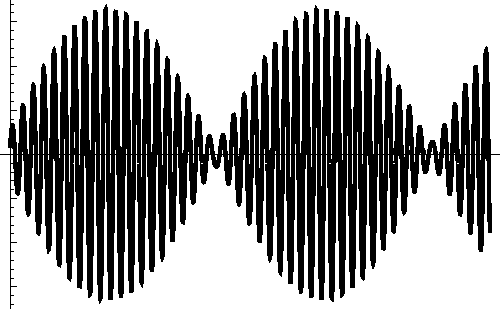
\includegraphics[width=\marginparwidth]{06-Non-Homogeneous-ODEs/resonnance}
\\
This is a typical graph of a solution with resonance. In this example, $w = 2$, $m=1.1$, $c\approx 0$, and $k=4$.  Since $\omega_0=\sqrt{4/1.1}\approx 2=\omega$, the quantity $\ds\frac{F_0}{m(\omega_0^2-\omega^2)}$ has a small denominator, which results in large periodic oscillations. If the oscillations are too large, they will destroy the system.
}}
As $\omega\to\omega_0$, the amplitude of the particular solution approaches infinity, and so we have extremely large oscillations (often called resonance). When the two frequencies are extremely close together, resonance can result in huge oscillations which can tear apart a mechanical system almost instantly. Notice in the picture on the right how the solution  

As a side note, the word frequency is used in different ways in different places. Always attach either circular or natural to the word frequency to convey the correct idea.
\begin{itemize}
\item The circular (angular) frequency, is $\omega_0 = \sqrt{k/m}$ (radians per second).
\item The natural frequency is $f = \frac{\omega_0}{2\pi}$ (hertz).
\end{itemize}
The period (distance from one peak to the next) is always interpret as the reciprocal of the natural frequency, $T=1/f$.
\end{observation}

\begin{observation}
If $c=0$ and $w=\omega_0 = \sqrt{k/m}$, then the modification rule applies and we use the method of undetermined coefficients to find $a$ and $b$ in $y_p=t(a\cos(\omega_0 t)+b\sin(\omega_0 t))$ (notice the $t$ in front). The solution is 
$$y_p(t) = \frac{F_0}{2m\omega_0}t\sin(\omega_0 t).$$ The $t$ in this solution causes the amplitude of the vibration to grow,  increasing without bound in a linear fashion. In this setting, any system will destroy itself as the oscillations will become too large to physically keep the system together. 

\marginpar{{
%\begin{figure}[h]
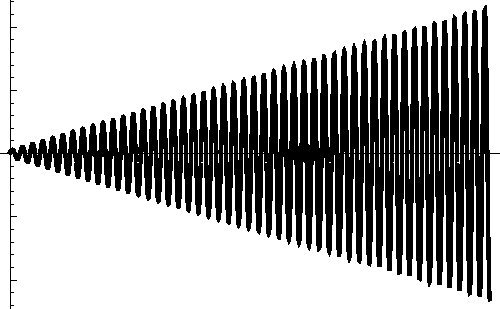
\includegraphics[width=\marginparwidth]{06-Non-Homogeneous-ODEs/growing-oscillation}

When $\omega_0=\omega$ and friction is negligible, a system will oscillate with an amplitude that grows without bound. Beware of this situation, as any mechanical system which undergoes this kind of oscillation will self destruct. 
%\end{figure}
}}
Anytime a mechanical system is built, the builders must study the internal frequencies of the system and make sure that they will not match external forces applied to the system. Soldiers marching across a bridge have collapsed a bridge in the past, so now it is common for soldiers to stop marching and shuffle across a bridge to prevent it from collapsing. The Tacoma Narrows bridge collapsed from forces due to resonance. Engineers must pay attention to both internal and external forces, making sure to avoid resonance.  
\end{observation}

\section{Electric circuits} (This section is largely a summary of page 116 from Schaum's Outlines.)
Kirchoff's Voltage law states that the voltage (electromotive force) impressed on a closed loop is equal to the sum of the voltage drops across the other elements of the loop. We use the expression $I(t)$ to represent the current in a loop. The following table illustrates summarizes the three types of voltage drops we will study.
\begin{center}
\begin{tabular}{|l|l|l|}
\hline
Component & Voltage drop & Other\\\hline
Resistor & $RI$ & Ohm's law, where $R$ is in ohms\\\hline
Inductor & $LI' = L(dI/dt)$ & $L$ is in henrys\\\hline
Capacitor& $Q/C$ & $Q$ is in coulombs, $C$ in farads.\\\hline
\end{tabular}
\end{center}
Here $Q$ is the charge on the capacitor, related to the current by $I(t)=\frac{dQ}{dt}$, or $Q=\int I(t) dt$.


\marginpar{{
\begin{center}
\renewcommand{\myscale}{.3}
\begin{tikzpicture}[scale=\myscale,inner sep=1pt]
%\draw[help lines,step=1cm] (0,0) grid (12,6);

%Source - like a battery
\node[label=right:$E$] at (0,3) 
{{\begin{tikzpicture}[scale=\myscale]
%	\useasboundingbox (-.5,-3) rectangle (.5,3);
	\draw (0,0) circle (1cm);
	\draw (.3,.5) -- (-.3,.5);
	\draw (0,.2) -- (0,.8);
	\draw (.3,-.5) -- (-.3,-.5);
	\draw (0,1) -- (0,3);
	\draw (0,-1) -- (0,-3);
	\end{tikzpicture}
}};

%Resistor
\node[label=right:$R$] at (6,3) 
{{\begin{tikzpicture}[scale=\myscale]
%	\useasboundingbox (0,-3) rectangle (0,3);
	\draw (0,-3) -- ++(0,1.8) -- ++(.5,.2) 
		-- ++(-1,.4) -- ++(1,.4)
		-- ++(-1,.4) -- ++(1,.4)
		-- ++(-1,.4) -- ++(.5,.2)
		-- ++(0,1.8) ;
	\end{tikzpicture}
}};

%Straight Path
%\node at (3,6) 
%{{\begin{tikzpicture}[scale=\myscale,rotate=90]
%	\draw (0,-3) -- (0,3);
%	\end{tikzpicture}
%}};

%Arrow to represent Current
\node[label=right:$i$] at (0,5) 
{{\begin{tikzpicture}[scale=\myscale,rotate=0]
	\filldraw (0,.4) -- (-.2,-.4) -- (0,-.3) -- (.2,-.4);
	\end{tikzpicture}
}};

%Loops
\node[label=above:$L$] at (3,6) 
{{\begin{tikzpicture}[scale=\myscale,rotate=90]
	\useasboundingbox (-.5,-3) rectangle (.5,3);
	\draw (0,-3) -- ++(0,1.5) 
	.. controls+(15:.2) and +(-90:.25) .. ++(.5,.4) 
	.. controls+(90:.25) and +(-15:.2) .. ++(-.5,.4) 
	.. controls+(-15:-.2) and +(90:.1) .. ++(-.5,-.05) 
	.. controls+(-90:.1) and +(15:-.2) .. ++(.5,-.05) 
	.. controls+(15:.2) and +(-90:.25) .. ++(.5,.4) 
	.. controls+(90:.25) and +(-15:.2) .. ++(-.5,.4) 
	.. controls+(-15:-.2) and +(90:.1) .. ++(-.5,-.05) 
	.. controls+(-90:.1) and +(15:-.2) .. ++(.5,-.05) 
	.. controls+(15:.2) and +(-90:.25) .. ++(.5,.4) 
	.. controls+(90:.25) and +(-15:.2) .. ++(-.5,.4) 
	.. controls+(-15:-.2) and +(90:.1) .. ++(-.5,-.05) 
	.. controls+(-90:.1) and +(15:-.2) .. ++(.5,-.05) 
	.. controls+(15:.2) and +(-90:.25) .. ++(.5,.4) 
	.. controls+(90:.25) and +(-15:.2) .. ++(-.5,.4) 
	-- (0,3);
	\end{tikzpicture}
}};


%Capacitor
\node[label=above:$C$] at (3,0) 
{{\begin{tikzpicture}[scale=\myscale,rotate=90]
%	\useasboundingbox (0,-3) rectangle (0,3);
	\draw (0,-3) -- ++(0,2.8) 
		-- ++(.5,0) -- ++(-1,0) 
		++(0,.4) -- ++(1,0)
		-- ++(-.5,0) -- ++(0,2.8);
	\end{tikzpicture}
}};


\end{tikzpicture}

\\
An $RLC$-circuit
\\
\vspace{.2in}
\renewcommand{\myscale}{.3}
\begin{tikzpicture}[scale=\myscale,inner sep=1pt]
%\draw[help lines,step=1cm] (0,0) grid (12,6);

%Source - like a battery
\node[label=right:$E$] at (0,3) 
{{\begin{tikzpicture}[scale=\myscale]
%	\useasboundingbox (-.5,-3) rectangle (.5,3);
	\draw (0,0) circle (1cm);
	\draw (.3,.5) -- (-.3,.5);
	\draw (0,.2) -- (0,.8);
	\draw (.3,-.5) -- (-.3,-.5);
	\draw (0,1) -- (0,3);
	\draw (0,-1) -- (0,-3);
	\end{tikzpicture}
}};

%Resistor
\node[label=right:$R$] at (6,3) 
{{\begin{tikzpicture}[scale=\myscale]
%	\useasboundingbox (0,-3) rectangle (0,3);
	\draw (0,-3) -- ++(0,1.8) -- ++(.5,.2) 
		-- ++(-1,.4) -- ++(1,.4)
		-- ++(-1,.4) -- ++(1,.4)
		-- ++(-1,.4) -- ++(.5,.2)
		-- ++(0,1.8) ;
	\end{tikzpicture}
}};

%Straight Path
\node at (3,6) 
{{\begin{tikzpicture}[scale=\myscale,rotate=90]
	\draw (0,-3) -- (0,3);
	\end{tikzpicture}
}};

%Arrow to represent Current
\node[label=above:$i$] at (3,6) 
{{\begin{tikzpicture}[scale=\myscale,rotate=-90]
	\filldraw (0,.4) -- (-.2,-.4) -- (0,-.3) -- (.2,-.4);
	\end{tikzpicture}
}};

%Inductor
%\node[label=above:$L$] at (3,6) 
%{{\begin{tikzpicture}[scale=\myscale,rotate=90]
%	\useasboundingbox (-.5,-3) rectangle (.5,3);
%	\draw (0,-3) -- ++(0,1.5) 
%	.. controls+(15:.2) and +(-90:.25) .. ++(.5,.4) 
%	.. controls+(90:.25) and +(-15:.2) .. ++(-.5,.4) 
%	.. controls+(-15:-.2) and +(90:.1) .. ++(-.5,-.05) 
%	.. controls+(-90:.1) and +(15:-.2) .. ++(.5,-.05) 
%	.. controls+(15:.2) and +(-90:.25) .. ++(.5,.4) 
%	.. controls+(90:.25) and +(-15:.2) .. ++(-.5,.4) 
%	.. controls+(-15:-.2) and +(90:.1) .. ++(-.5,-.05) 
%	.. controls+(-90:.1) and +(15:-.2) .. ++(.5,-.05) 
%	.. controls+(15:.2) and +(-90:.25) .. ++(.5,.4) 
%	.. controls+(90:.25) and +(-15:.2) .. ++(-.5,.4) 
%	.. controls+(-15:-.2) and +(90:.1) .. ++(-.5,-.05) 
%	.. controls+(-90:.1) and +(15:-.2) .. ++(.5,-.05) 
%	.. controls+(15:.2) and +(-90:.25) .. ++(.5,.4) 
%	.. controls+(90:.25) and +(-15:.2) .. ++(-.5,.4) 
%	-- (0,3);
%	\end{tikzpicture}
%}};


%Capacitor
\node[label=above:$C$] at (3,0) 
{{\begin{tikzpicture}[scale=\myscale,rotate=90]
%	\useasboundingbox (0,-3) rectangle (0,3);
	\draw (0,-3) -- ++(0,2.8) 
		-- ++(.5,0) -- ++(-1,0) 
		++(0,.4) -- ++(1,0)
		-- ++(-.5,0) -- ++(0,2.8);
	\end{tikzpicture}
}};


\end{tikzpicture}

\\
An $RC$-circuit
\\
\vspace{.2in}
\renewcommand{\myscale}{.3}
\begin{tikzpicture}[scale=\myscale,inner sep=1pt]
%\draw[help lines,step=1cm] (0,0) grid (12,6);

%Source - like a battery
\node[label=right:$E$] at (0,3) 
{{\begin{tikzpicture}[scale=\myscale]
%	\useasboundingbox (-.5,-3) rectangle (.5,3);
	\draw (0,0) circle (1cm);
	\draw (.3,.5) -- (-.3,.5);
	\draw (0,.2) -- (0,.8);
	\draw (.3,-.5) -- (-.3,-.5);
	\draw (0,1) -- (0,3);
	\draw (0,-1) -- (0,-3);
	\end{tikzpicture}
}};

%Resistor
\node[label=right:$R$] at (6,3) 
{{\begin{tikzpicture}[scale=\myscale]
%	\useasboundingbox (0,-3) rectangle (0,3);
	\draw (0,-3) -- ++(0,1.8) -- ++(.5,.2) 
		-- ++(-1,.4) -- ++(1,.4)
		-- ++(-1,.4) -- ++(1,.4)
		-- ++(-1,.4) -- ++(.5,.2)
		-- ++(0,1.8) ;
	\end{tikzpicture}
}};

%Straight Path
\node at (3,0) 
{{\begin{tikzpicture}[scale=\myscale,rotate=90]
	\draw (0,-3) -- (0,3);
	\end{tikzpicture}
}};

%Arrow to represent Current
\node[label=above:$i$] at (3,0) 
{{\begin{tikzpicture}[scale=\myscale,rotate=90]
	\filldraw (0,.4) -- (-.2,-.4) -- (0,-.3) -- (.2,-.4);
	\end{tikzpicture}
}};

%Inductor
\node[label=above:$L$] at (3,6) 
{{\begin{tikzpicture}[scale=\myscale,rotate=90]
	\useasboundingbox (-.5,-3) rectangle (.5,3);
	\draw (0,-3) -- ++(0,1.5) 
	.. controls+(15:.2) and +(-90:.25) .. ++(.5,.4) 
	.. controls+(90:.25) and +(-15:.2) .. ++(-.5,.4) 
	.. controls+(-15:-.2) and +(90:.1) .. ++(-.5,-.05) 
	.. controls+(-90:.1) and +(15:-.2) .. ++(.5,-.05) 
	.. controls+(15:.2) and +(-90:.25) .. ++(.5,.4) 
	.. controls+(90:.25) and +(-15:.2) .. ++(-.5,.4) 
	.. controls+(-15:-.2) and +(90:.1) .. ++(-.5,-.05) 
	.. controls+(-90:.1) and +(15:-.2) .. ++(.5,-.05) 
	.. controls+(15:.2) and +(-90:.25) .. ++(.5,.4) 
	.. controls+(90:.25) and +(-15:.2) .. ++(-.5,.4) 
	.. controls+(-15:-.2) and +(90:.1) .. ++(-.5,-.05) 
	.. controls+(-90:.1) and +(15:-.2) .. ++(.5,-.05) 
	.. controls+(15:.2) and +(-90:.25) .. ++(.5,.4) 
	.. controls+(90:.25) and +(-15:.2) .. ++(-.5,.4) 
	-- (0,3);
	\end{tikzpicture}
}};


%Capacitor
%\node[label=above:$C$] at (3,0) 
%{{\begin{tikzpicture}[scale=\myscale,rotate=90]
%	\draw (0,-3) -- ++(0,2.8) 
%		-- ++(.5,0) -- ++(-1,0) 
%		++(0,.4) -- ++(1,0)
%		-- ++(-.5,0) -- ++(0,2.8)
%	\end{tikzpicture}
%}};


\end{tikzpicture}

\\
An $RL$-circuit
\end{center}}}
In a circuit  with one resistor, one inductor, and one capacitor (an $RLC$ circuit), if the electromotive force is $E(t)$, then Kirchoff's Voltage law gives the integro-differential equation 
$$L I'+ RI+ \frac{1}{C}Q(t) =E(t) \quad \text{or}\quad L I'+ RI+ \frac{1}{C}\int I(t) dt = E(t).$$  
Differentiating both sides removes the integral and gives
$$L I''+ RI'+ \frac{1}{C}I(t) = E'(t),$$ which is a 2nd order non homogeneous linear differential equation with constant coefficients. 
If the electromotive force is sinusoidal (such as $E(t) = E_0\sin(\omega t)$), then we can solve this differential equation to find the current exactly the same way we did in the last section. Notice however that initial conditions will most often be given in terms of initial charge $Q(0)$ and initial current $I(0)$.  To solve the differential equation, you will have to use the first equation $ L I'(t)+ RI(t)+ \frac{1}{C}Q(t) =E(t)$ to obtain a value for $I'(0)$

Due to time constraints, I will let you read the examples in the text for examples involving specific $RLC$, $RC$, and $RL$ circuits. When working with $RC$-circuits, you differentiate both sides to obtain a first order ODE, and initial conditions are generally given as initial charge.  When working with an $RL$-circuit, you don't need to differentiate $E(t)$, and the initial current is generally given for initial conditions. One key observation to make is that when you are given initial conditions for the charge and current, you use these to find initial conditions for the current's derivative. Even when $Q(0)=0$ and $I(0)=0$, we may find that $I'(0)\neq 0$. Use the equation involving $Q$ to find $I'(0)$. (Problem 14.13 provides an excellent example of how this can occur.) 

\section{Comparing the two models - saving money}

Mechanical models are expensive to build.  Electrical models are fairly simple to build and measure.  If you need to create a mechanical system, it may prove beneficial financially to start with an electrical model. Engineers spend another semester on this idea in system dynamics.  Hydraulic systems are also very closely related. In bridging between mechanical and electrical systems, we compare the following variables. 

\begin{center}
\begin{tabular}{|c|c|c|c|c|c|}
\hline
Mechanical System&$m$&$c$&$k$&$r(t)=F_0\cos\omega t$&$y(t)$\\\hline
Electrical System&$L$&$R$&$1/C$&$E'(t) = E_0\omega\cos\omega t$&$I(t)$\\
\hline
\end{tabular}
\end{center}

Solving a problem in one system (either mechanical or electrical) can provide useful results in the other.  


\newgeometry{left=1in,right=1in,top=1in,bottom=1in}
\section{Preparation}

\noindent  
This chapter covers the following ideas. When you create your lesson plan, it should contain examples which illustrate these key ideas. Before you take the quiz on this unit, meet with another student out of class and teach each other from the examples on your lesson plan. 


\begin{enumerate}
	\item Explain Hooke's Law in regards to mass-spring systems, where there is an external force. Construct and solve differential equations which represent this physical model, with or without the presence of a damper and be able to interpret how solutions change based on changes in the model. 
	\item Understand the theory which relates solutions of homogeneous linear ODE's to non homogeneous ODEs. 
	\item Use the method of undetermined coefficients  to solve non homogeneous linear ODEs.
	\item Explain Kirchhoff's voltage law, Ohm's law, and how to model electrical circuits using 2nd order non homogeneous linear ODEs.  Illustrate how results about circuits can be translated into results about mass-spring systems.


\end{enumerate}




Here are the preparation problems for this unit.  All of these problems come from Schaum's Outlines.
\begin{center}
\begin{tabular}{ll}
&Preparation Problems\\
\hline\hline
Day 1& 8.21, 11.1, 11.2, 11.3
\\\hline
Day 2& 11.9,10, 13.7, 14.10 
\\\hline
Day 3& 14.12, 14.13, 14.46, 14.54 
\\\hline
Day 4& Lesson Plan, Quiz
\\\hline
\end{tabular}
\end{center}


Here are the homework problems which line up with the material we are learning. Remember your assignment is to do at least 7 per day (2 of those with Mathematica).  On the application problems, graph your solutions so that you can see what is going on.


\begin{center}
\begin{tabular}{|l|c|l|l|l|l|}
\hline
Concept&Sec&Suggestions&Relevant Problems\\ \hline
Theory&8&21,65&21-23,65-67\\ \hline
Undetermined Coef&11&1,2,3,8,10,24,26,34,36,41,46,47,48&All\\ \hline
IVP&13&1,7,14&1,3,7,8,10,11,14\\ \hline
Applications&7&19,76&19-22,71-81\\ \hline
Applications&14&10,11,13,14,17,46,50,51,52,54,57&9-18,44-65\\ \hline
\end{tabular}
\end{center}



\restoregeometry



\chapter{Laplace Transforms}

%Notes to self:  The order here needs revamping.  Here is a suggestion.  Try starting with talking about the general idea (we convert an ODE to something we can solve with algebra, then solve it, and then convert back).  Give them the Laplace transform of $1, t, e^t, \sin t, \cos t$. Then give them the derivative rules through 2nd derivative, and solve 2 ODEs (one first order and one second order).  Show how the process is carried out in general.  Then postpone any more ODE problems until after you get in the first and second shifting theorems and the Dirac-delta distribution.  Then focus on IVP's which require partial fractions or completing the square.  After some practice with all of these ideas, finally introduce the convolution theorem.  This will probably take 5 days.  It took me 6 plus to get it all out when I do it in the wrong order.

%Based upon the way students study in my class, it might be nice to have a quiz on this stuff immediately after introducing the Laplace transform, and then add in solving ODEs. However, this would just help those who procrastinate doing homework until the day before the quiz. Maybe that is not what is needed.  Doing problems in class requires that students recognize patterns, and will only be doable once students have practiced the material. In other words, class time will be severely affected by students who do not practice.

%What I have noticed is that students do not attempt the material until right before the quiz.  Hence, if you start with ODEs, then they are lost with the Laplace Transform part, and can't even start on the ODEs.  Hence, this section can be a time sink in the course, because students didn't practice things right away. Pattern recognition here becomes crucial.  The problems in our text perhaps need some work as well, so that students can practice taking Laplace Transforms. (More simple pattern recognition problems would be nice.)

This chapter covers the following ideas. When you create your lesson plan, it should contain examples which illustrate these key ideas. Before you take the quiz on this unit, meet with another student out of class and teach each other from the examples on your lesson plan. 


\begin{enumerate}

\item Explain how to compute Laplace transforms and inverse Laplace transforms. Explain and use both shifting theorems, and be able to prove them. 
\item Use Laplace transforms to solve IVP's.
\item Describe the Dirac delta function, and use it in solving ODEs. Illustrate what the Dirac delta function does to a system by applying it to examples in mass-spring systems and electrical networks.
\item Explain what a convolution is, and how it relates to Laplace transforms. Be able to use the Transform theorems related to differentiating and integrating functions or their transforms.

\end{enumerate}




\section{The big idea}
The Laplace transform is a tool which became popular in the last 100 years because of the work of engineers.  The Laplace transform has the ability to convert a differential equation into an algebraic equation which can be solved purely with algebra.  The Laplace transform can be applied to functions which are not continuous, which makes it extremely useful in real world applications. For example, if a hammer hits a mass-spring system, or an electrical switch is turned on or off, the Laplace transform can handle the complications which these simple changes bring to an ODE.  The methods we have learned before require that our driving forces are continuously differentiable functions.

The big idea in this unit is a three step process.
\begin{enumerate}
	\item Convert and ODE into an algebraic equation using the Laplace transform.
	\item Solve the corresponding algebraic equation (which often means you have to use a partial fraction decomposition and completing the square).
	\item Use an inverse Laplace transform to find the solution of the ODE.
\end{enumerate}
The first part of this unit will focus on finding Laplace transforms and their inverses. The second part will focus on solving ODEs. The third part will focus on what happens when we apply impulses to a system (such as a hammer blow, or a bolt of lightning). The fourth part will focus on some theoretical aspects of the Laplace Transform.
 

\section{Finding Laplace Transforms and Their Inverses}
The Laplace transform of a function $f(t)$ defined for $t\geq 0$ is $F(s)=L(f(t))=\int_0^\infty e^{-st}f(t)dt$. The function $f(t)$ is called the inverse Laplace transform of $F(s)$, and we write $f(t)=L^{-1}(F(s))$. As a notational convenience, we use lower case letters and $t$ to describe original functions, and the same capital letter and $s$ to represent the Laplace transform. Provided the function $f$ is ``nice'' (of exponential order, see pg 448), it will have a Laplace transform for large enough $s$.

\subsection{Finding the Laplace Transform}
If $f(t)=1$, then $F(s)=\int_0^\infty e^{-st}1dt= \frac{e^{-st}}{-s}\big|_0^\infty = \frac{1}{s}$, provided $s>0$. If $f(t)=e^{at}$, then $F(s)=\int_0^\infty e^{-st}e^{at}dt=\int_0^\infty e^{-(s-a)t}dt= \frac{e^{-(s-a)t}}{-(s-a)}\big|_0^\infty = \frac{1}{s-a}$, provided $s>a$. The improper integral computed with the Laplace transform will normally exist only for certain values of $s$. 

Since integration can be done term by term, we have $L(af+bg)=aL(f)+bL(g)$ for functions $f,g$ and constants $a,b$.  We can use this to find many other Laplace transforms without having to do any more integration. We have $L(\cosh a t) = \frac{1}{2}L(e^{at}+L(e^{-a t}))=\frac{1}{2}\left(\frac{1}{s-a}+\frac{1}{s+a}\right) = \frac{s}{s^2-a^2}$. Similarly $L(\sinh a t) = \frac{a}{s^2-a^2}$.  

\begin{wraptable}[5]{r}{0pt}
\begin{tabular}{|c|c|c|}
\hline
&$D$&$I$\\\hline
$+$&$\cos \omega t$&$e^{-st}$\\
$-$&$-\omega \sin \omega t$&$e^{-st}/(-s)$\\
$+$&$-\omega^2 \cos \omega t$&$e^{-st}/s^2$\\\hline
\end{tabular}
\end{wraptable}

Integration by parts twice yields $L(\cos \omega t) = \frac{s}{s^2+\omega^2}$ and $L(\sin \omega t) = \frac{\omega}{s^2+\omega^2}$. To see this, write $L(\cos \omega t) = \int_0^\infty e^{-st}\cos \omega t dt$.  The tabular method gives $\int_0^\infty e^{-st}\cos \omega t dt = \left(\cos \omega t e^{-st}/(-s) +\omega \sin \omega te^{-st}/s^2\right)\big|_0^\infty - \int_0^\infty \omega^2 \cos \omega te^{-st}/s^2dt = 1/s - \omega^2/s^2 \int_0^\infty e^{-st}\cos \omega t dt$, which means $L(\cos \omega t) = 1/s-\omega^2/s^2L(\cos \omega t)$. This means $(1+\omega^2/s^2)L(\cos \omega t) = \frac{1}{s}$, or $(s^2+\omega^2) L(\cos \omega t)=s$ or $L(\cos \omega t)=\frac{s}{s^2+\omega^2}$. Integration by parts also shows that $L(t^n) = \frac{n!}{s^{n+1}}$ for integers $n$. 

%
%The Gamma function, defined as $\Gamma(x) = \int_0^\infty e^{-t}t^{x-1}dt$, shows up in the formula $L(t^a) = \frac{\Gamma(a+1)}{s^{a+1}}$. We can calculate $\Gamma(1)=1$. Integration by parts show that $\Gamma(n+1) = \int_0^\infty e^{-t}t^{n}dt = (-t^{n}e^{-t})\big|_0^\infty + n\int_0^\infty e^{-t}t^{n-1}dt = n\Gamma(n)$. Hence we can show that $\Gamma(2)=\Gamma(1+1)=1\Gamma(1)=1$, $\Gamma(3)=\Gamma(2+1)=2\Gamma(2)=2!$, $\Gamma(4)=\Gamma(3+1)=3\Gamma(3)=3\cdot 2! = 3!$, and $\Gamma(n+1)=\Gamma(n+1)=n\Gamma(n)=n!$. In more advanced texts, it is shown that $\Gamma(1/2)=\sqrt{\pi}$. This can be used to find Laplace Transforms of $t^{n/2}$.  For example, $L(t^{1/2})=\frac{\Gamma(1/2) }{s^{3/2}} = \frac{\sqrt{\pi}}{s^{3/2}}$.  The Laplace transform of $t^{3/2}$ requires the computation $\Gamma{3/2} = \frac{1}{2}\Gamma(\frac{1}{2}) = \frac{1}{2}\sqrt{\pi}$.

For convenience, the following table summarizes the Laplace Transforms we will use most often.
\begin{center}
\begin{tabular}{|r|c|c|c|c|c|c|c|c|}
\hline
$f(t)$ & $t^n$        & $t^0=1$        &$e^{at}$   & $\cos(wt)$     &$\sin(wt)$     & $\cosh(wt)$    &$\sinh(wt)$   &$u(t-a)$
\\\hline 
 F$(s)$& $n!/s^{n+1}$  & $1/s$  &$1/(s-a)$  & $s/(s^2+w^2)$  &$w/(s^2+w^2)$  & $s/(s^2-w^2)$  &$w/(s^2-w^2)$ &$e^{-as}/s$
\\
          &$s>0$         &$s>0$         &$s>a$      &$s>0$           &$s>0$          &$s>|w|$         &$s>|w|$       & $s>0$
\\\hline
\end{tabular}
\end{center}


\subsection{Finding an Inverse Laplace Transform}
If the Laplace transforms of two functions are the same, then the two function must be the same as well. This allows us to invert the Laplace transform and obtain the only function with a given Laplace transform.  Inverting a Laplace transform often involves matching the transformed function up with a function from a table, and then using the table to invert the transform.  

To find the inverse Laplace transform of $F(s) = \frac{7}{s^3}$, first notice that $\frac{2}{s^3}$ is the transform of $t^2$. We rewrite $F(s) = \frac{7}{s^3} = \frac{7}{2}\frac{2!}{s^3}$, and then find the inverse transform as $L^{-1}(F(s)) = \frac{7}{2}t^2$.

To find the inverse Laplace transform of $F(s) = \frac{3s+4}{s^2+25}$, we notice that the transforms of $\cos(5t)$ and $\sin(5t)$ are $s/(s^2+5^2)$ and $5/(s^2+5^2)$.  We rewrite $F(s)  = \frac{3s+4}{s^2+25}= 3\frac{s}{s^2+25} +\frac{4}{5} \frac{5}{s^2+25} $, and then the inverse transform is $3\cos(5t)+\frac{4}{5}\sin(5t)$.

To find the inverse Laplace transform of $F(s) = \frac{3s+1}{s^2+3s+2}$, we start by factoring the denominator as $(s^2+3s+2) = (s+2)(s+1)$.  We then use a partial fraction decomposition to write $\frac{3s+1}{s^2+3s+2} = \frac{A}{s+2}+\frac{B}{s+1}$. Multiplication on both sides by $s^2+3s+2$ gives $(3)s+(1) = A(s+1)+B(s+2) = (A+B)s+(A+2B)$.  Since the left and right sides are both linear equations of $s$, the coefficients must be equal so we must have $3=A+B$ and $1=A+2B$. The solution is $B=-2$ and $A=5$.  This means that $F(s) = 5\frac{1}{s+2}-2\frac{1}{s+1}$, which means the Laplace inverse is $f(t) = 5e^{-2t}-2e^{-t}$.

\subsection{Shifting Theorems and The Heaviside Function}

\subsubsection{$s$-shifting: Multiplication by $e^{at}$}

The $s$-shifting theorem states that $$F(s-a) = L(e^{at}f(t))$$ or alternatively $L^{-1}(F(s-a)) = e^{at}f(t)$. For example, $L(e^{3t}\cos(\pi t)) = \frac{s-3}{(s-3)^2+\pi^2}$. In other words, multiplication of the function $f(t)$ by $e^{at}$ means that you first find the Laplace transform of $f$ and the replace each $s$ with $s-a$. As a quick example, we compute $L(t^2e^{-5t}) = \frac{2!}{(s+5)^3}$ (start by finding $L(t^2)=\frac{2!}{s^3}$ and the replace the $s$ with $s-(-5)$).

The inverse Laplace transform of $\frac{3}{(s-4)^3}$ is related to the inverse transform of $\frac{3}{s^3}$. The transform of $t^2$ is $\frac{2}{s^3}$, so the inverse transform of $\frac{3}{s^3}=\frac{3}{2}\frac{2}{s^3}$ is $\frac{3}{t}t^2$.  Because there was an $s-4$ in the original denominator, we have to multiply by $e^{4t}$ to obtain the inverse Laplace transform of $\frac{3}{(s-4)^3}$ as $\frac{3}{t}t^2e^{4t}$.  

The inverse Laplace transform of $\frac{s-2}{(s-4)^2+1}$ is found by first obtaining an $s-4$ in the numerator and then breaking the fraction into two parts, $\frac{s-4+4-2}{(s-4)^2+1} = \frac{s-4}{(s-4)^2+1}+2\frac{1}{(s-4)^2+1}$. We then compute the inverse transform as $e^{4t}\cos(t) + 2e^{4t}\sin(t)$.  

To use the $s$ shifting theorem, you have to get good at adding zero to a problem (as I did in the previous example with $-4+4$). You may have to complete the square in the denominator, as $\frac{s+2}{s^2+4s+13} = \frac{s+2}{(s+2)^2+9}$ has Laplace inverse $e^{-2t}\cos 3t$. The reason the shifting theorem is true is because (here's the 3 step short proof) $$ L(e^{at}f(t)) = \int_0^\infty e^{-st}(e^{at}f(t))dt = \int_0^\infty e^{-(s-a)t}f(t)dt = F(s-a).$$ 


\subsubsection{The Heaviside function and $t$-shifting  (Multiplication by $e^{-as}$)}
The Heaviside function $u(t) = \begin{cases}0 &t<0 \\ 1 &t\geq 0\end{cases}$ can be though of as a function which turns  other functions on and off.  For example, the function $t^2u(t)$ is zero to the left of $0$, and then the function $t^2$ is turned on at $t=0$.  The function $t^2(u(t)-u(t-3))$ turns on the function $t^2$ at $t=0$ and then turns it off at $t=3$. The Heaviside function can be used to piece together piecewise continuous functions by using this ``on-off'' approach.  For example, the function 
$f(t) = 
\begin{cases}
0 &t<0 \\ 
t^2& 0\leq t\leq 1\\
2-t & 1< t\leq \pi\\
\cos t & \pi< t
\end{cases}$ can be written using the Heaviside function as $f(t) = t^2[u(t)-u(t-1)] + (2-t)[u(t-1)-u(t-\pi)]+\cos t [u(t-\pi)]$.  This section describes how to compute Laplace transforms and inverse transforms of such piecewise defined functions.  Such functions are needed to model turning on a switch in an electrical network, modifying the driving force in a mechanical spring system, and many other practical applications.



The $t$-shifting theorem states $$L(f(t-a)u(t-a))=e^{-as}F(s)$$ or $L^{-1}(e^{-as}F(s)) = f(t-a)u(t-a)$, where $F(s)=L(f(t))$. This theorem is easiest to use when computing inverse transforms, as it says that multiplication of $F(s)$ by $e^{-as}$ means that you multiply the inverse of $F(s)$ by $u(t)$ and then replace all the $t$'s with $t-a$. For example we can find the inverse transform of $F(s) = \frac{2}{s^2+4}e^{-3s}$ by first noting that the inverse transform of $\frac{2}{s^2+4}$ is $\sin(2t)$, and so we multiply by $u(t)$ and replace each $t$ with $t-3$ to obtain $L^{-1}(F(s))=\sin(2(t-3))u(t-3)$. This is just the curve $\sin(2t)$ which has been shifted $3$ units to the right and turned on at $t=3$. 

Notice that the $t$-shifting theorem has an $e^{-as}$, while the $s$ shifting theorem has an $e^{at}$. Pay attention to this sign difference. The reason the $t$-shifting theorem is true is because $\int_0^{\infty}f(t-a)u(t-a)e^{-st}dt = \int_a^\infty f(t-a)e^{-st}dt$. By the substitution $w=(t-a)$, this becomes $\int_0^\infty f(w)e^{-s{w+a}}dw = e^{-as}\int_0^\infty f(w)e^{-sw}dw = e^{-as}F(s)$. Again it is a fairly short proof.

To use the $t$-shifting theorem to compute forward Laplace transforms, you have to rewrite $f(t)$ in terms of $t-a$. For example, the function $t^2$ for $t>1 $ and 0 otherwise is written $f(t) = t^2 u(t-1)$. To use the second shifting theorem, we write $f(t) = t^2u(t-1) = ( (t-1)+1)^2u(t-1)= ((t-1)^2 +2(t-1)+1)2u(t-1)$. Notice how I purposefully inserted a $-1+1$ next to the $t$. The shifting theorem then gives $F(s)=\left(\frac{2}{s^3}+frac{2}{s^2}+\frac{1}{s}\right)e^{-s}$. Our function $f(t-1) =  (t-1)^2 +2(t-1)+1$ is simply $f(t) = t^2+2t+1$ whose transform is $\frac{2}{s^3}+frac{2}{s^2}+\frac{1}{s}$, which we then multiply by $e^{-s}$ to complete the transform. An alternate version of this transformation uses the formula $$L(f(t)u(t-a)) = e^{-as}L(f(t+a))$$ (meaning replace each $t$ with $t+a$ and then find the transform and multiply by $e^{-as}$).   This formula shows that $L(t^2u(t-1)) = e^{-s}L((t+1)^2) = e^{-s}L(t^2+2t+1)) = e^{-s} \left(\frac{2}{s^3}+\frac{2}{s^2}+\frac{1}{s}\right)$ as before.

Both shifting theorems can be applied simultaneously.  If $F(s) =\frac{(s-3)e^{-2s}}{(s-3)^2+\omega^2} $, then without the $e^{-2s}$ the inverse transform would be $e^{3t}\cos(\omega t)$ by the $s$-shifting theorem. The $t$-shifting theorem says that the inverse transform is $e^{3(t-2)}\cos(\omega(t-2))u(t-2)$ (multiply by $u(t)$ and then replace each $t$ with $t-2$). Remember that with the $s$ shifting theorem you change the sign, but with the $t$ shifting theorem you do not. This is the most common mistake.


\section{Solving IVPs}

\subsection{The Transform of a derivative}
The Laplace transform of a derivative is, using integration by parts, $$L(f^\prime)=\int_0^\infty e^{-st}f^\prime (t)dt = (e^{-st}f(t))\big|_0^\infty + s\int_0^\infty e^{-st}f (t)dt  = sL(f)-f(0).$$  We can use this formula to get $$L(f^{\prime\prime}) = sL(f^\prime)-f^\prime(0) = s[sL(f)-f(0)]-f^\prime(0) = s^2L(f) - sf(0)-f^\prime(0).$$  These two formulas can be used to find new Laplace transforms and (most importantly) solve ODEs.

%We now find the Laplace transform of $f(t)=t\cos 3t$ using these formulas.  We have $f^\prime = -3t\sin 3t +\cos 3t$ and $f^{\prime\prime} = -9t\cos 3t -6\sin 3t$. Notice that the second derivative contains the exact same $t\cos 3t$ term .  The formula $L(f^{\prime\prime}) = s^2L(f) - sf(0)-f^\prime(0)$ gives $L(-9t\cos t -6\sin t) = sL(t\cos 3t)-s(0)-1$, or $-9L(f) -6\frac{3}{s^2+9} = s^2L(f)-1$. Hence we have $L(f) = \frac{1}{s^2+9}-\frac{18}{(s^2+9)^2} = \frac{s^2-9}{(s^2+9)^2}$.

\subsection{Solving IVPs - Lots of examples}
We can use the differentiation theorem to solve IVPs. Given an ODE, take the Laplace transform of each side, giving what is called the subsidiary equation.  This equation can be solved for $L(y)=Y(s)$ using only algebra.  You then compute $L^{-1}(Y(s))$ to find the solution to the IVP $y(t)$.  This may involve finding a partial fraction decomposition. Laplace transforms reduce many IVPs to a 3 step process (1) convert to the subsidiary equation, (2) use algebra to solve for $Y$, performing a partial fraction decomposition if needed, (3) find inverse Laplace transform.

To solve the homogeneous IVP $y^\prime +2y =0, y(0)=1$ we start by taking the Laplace transform of each side. This gives the subsidiary equation $sL(y)-y(0)+2L(y) = 0$, or using the notation $L(y)=Y$, we have $sY-1+2Y=0$.  Solving for $Y$ gives the equation $Y=\frac{1}{s+2}$. The inverse Laplace transform of both sides gives $y(t) = e^{-2t}$.  

To solve the nonhomogeneous IVP $y^\prime +2y =3, y(0)=1$, take the Laplace transform of each side. This gives the subsidiary equation $sY-1+2Y=\frac{3}{s}$.  Solving for $Y$ gives the equation $Y=\frac{s+3}{s(s+2)}$. The partial fraction decomposition $\frac{s+3}{s(s+2)}=\frac{A}{s}+\frac{B}{s+2}$ requires we solve $s+3 = A(s+2)+Bs$, or $1=A+B, 3=2A$ giving  $A=3/2$ and $B=-1/2$. Our subsidiary equation is now $Y = \frac{3}{2}\frac{1}{s}-\frac{1}{2}\frac{1}{s+2}$. The inverse Laplace transform of both sides gives $y(t) = \frac{3}{2}-\frac{1}{2}e^{-2t}$. These two examples represent the basic ideas used to solve pretty much every Laplace transform problem. 

Now for a problem with a Heaviside function. Consider the IVP $y^{\prime\prime} +4y =u(t-5), y(0)=0,y^\prime(0)=1$, which represents a mass-spring system with no friction which has a constant driving force of magnitude 3 applied at time $t=5$. Take the Laplace transform of each side to obtain. $s^2Y-sy(0)-y^\prime(0) +4Y=\frac{e^{-4s}}{s}$ or $(s^2+4)Y=1+\frac{e^{-5s}}{s}$.  Solving for $Y$ gives the equation $Y=\frac{1}{s^2+4}+\frac{1}{s(s^2+4)}e^{-5s}$. The partial fraction decomposition $\frac{1}{s(s^2+4)}=\frac{A}{s}+\frac{Bs+C}{s^2+4}$ becomes $0s^2+0s+1 = A(s^2+4)+Bs^2+Cs = (A+B)s^2+(C)s+(4A)$. We obtain the 3 equations $0=A+B, 0=C, 1=4A$ whose solution is  $A=1/4,B=-1/4,C=0$. Our subsidiary equation is now $Y=\frac{1}{2}\frac{2}{s^2+4}+\left[\frac{1}{4}\frac{1}{s}-\frac{1}{4}\frac{s}{s^2+4}\right]e^{-5s}$. The inverse Laplace transform of both sides gives $y(t) =\frac{1}{2}\sin(2t)+[\frac{1}{4}-\frac{1}{4}\cos(2(t-5))]u(t-5)$, using the $t$-shifting theorem. 

For a more involved example, to solve the IVP $y^{\prime\prime}+4y^\prime+3y=30e^{2t}, y(0)=1, y^\prime(0)=3$, take the Laplace transform of each side. This gives the subsidiary equation $s^2Y - sy(0)-y^\prime(0)+4(sY-y(0))+3Y=\frac{30}{s-2}$. Solving for $Y$ gives us $(s^2+4s+3)Y=s+7+\frac{30}{s-2}$ or 
$$Y(s) 
= \frac{s+7}{s^2+4s+3} + \frac{30}{(s^2+4s+3)(s-2)}
= \frac{(s+7)(s-2)+30}{(s+1)(s+3)(s-2)} = \frac{s^2+5s+16}{(s+1)(s+3)(s-2)}.$$ A partial fraction decomposition gives $\frac{A}{s+1} +\frac{B}{s+3}+\frac{C}{s-2}$. Multiplying both sides by $(s+1)(s+3)(s-2)$ gives $s^2+5s+16 = A(s+3)(s-2)+B(s+1)(s-2)+C(s+1)(s+3) = A(s^2+s-6) +B(s^2-s-2)+C(s^2+4s+3)$.  We equate the coefficients of $x^2, x,$ and the constants on each side to get the three equations $1 = A+B+C, 5=A-B+4C, 16=-6A-2B+3C$. The solution to this system is $A=-2,B=1, C=2$, which means $Y(s) = \frac{-2}{s+1} +\frac{1}{s+3}+\frac{2}{s-2}$.  The inverse Laplace transform of $Y(s)$ is $L^{-1}(Y)= y(t) = -2e^{-t} + e^{-3t} +2e^{2t}$. An alternate way to do a partial fraction decomposition would be to consider the equation   $s^2+5s+16 = A(s+3)(s-2)+B(s+1)(s-2)+C(s+1)(s+3)$ and let $s=-3,2,-1$, which gives $10=B(10), 30=C(15), 12=A(-6)$, which gives the same numbers for $A,B,C$ as equating the coefficients.

Let's consider an example where a factor appears more than once in the denominator of a partial fraction decomposition.
To solve the ODE IVP $y^{\prime\prime}+4y^\prime+4y=0, y(0)=1, y^\prime(0)=3$, take Laplace transforms of both sides to obtain the subsidiary equation $s^2Y - sy(0) - y^\prime(0) + 4(sY - y(0)) + 4Y = 0$ or $s^2Y - s - 3 + 4(sY - 1) + 4Y = 0$. Solving for $Y$ gives $Y = \frac{s+7}{s^2+4s+4}=\frac{s+7}{(s+2)^2}$.  Since we have a double factor in the denominator, our partial fraction decomposition is $ \frac{s+7}{(s+2)^2} = \frac{A}{s+2}+\frac{B}{(s+2)^2}$, or $s+7 = A(s+2)+B = As+(2A+B)$. The solution to the system $A=1, 2A+B=7$ is $A=1,B=5$.  Hence our subsidiary equation is $Y = \frac{1}{s+2}+5\frac{1}{(s+2)^2}$.  The $t$-shifting theorem gives us the inverse transform $y=e^{-2t}+5te^{-2t}$. This is yet another reason why you multiply by $t$ when you get a repeated factor.  

In solving the ODE $y^{\prime\prime}+4y^\prime+5y=e^{-2t}\cos t, y(0)=0, y^\prime(0)=1$, our subsidiary equation would be $s^2Y-1+4sY+5Y = \frac{s+2}{(s+2)^2+1}$. Solving for $Y$ gives $Y = \frac{1(s^2+4s+5)+(s+2)}{((s+2)^2+1)^2} =  \frac{s^2+5s+7}{((s+2)^2+1)^2}$.  A partial fraction decomposition would be $\frac{s^2+5s+7}{((s+2)^2+1)^2} = \frac{As+B}{(s+2)^2+1}+ \frac{Cs+D}{((s+2)^2+1)^2}$, or $s^2+5s+7 = (As+B)(s^2+4s+5)+(Cs+D) = (A)s^3+(4A+B)s^2+(5A+4B+C)s+(5B+D)$.  This gives the system of equations $0=A,1=4A+B,5=5A+4B+C,5B+D=7$ which has solutions $A=0,B=1,C=1,D=2$. The subsidiary equation is hence $Y=\frac{1}{(s+2)^2+1}+ \frac{s+2}{((s+2)^2+1)^2}$ which has Laplace inverse $y=e^{-2t}\sin(t) + e^{-2t}\frac{t}{2}\sin(t)$ using the table of Laplace transforms on the front cover of your book. I would not expect you to carry out this last inverse without access to a table.

\subsection{How to handle initial conditions that are not at $t=0$}
If the initial conditions are not stated in terms of $t_0=0$, then change variables $\hat t = t-t_0$ so that the initial conditions are at $\hat t_0 =0$.  For example, to solve the IVP $y^{\prime\prime}+y=3, y(2)=0, y^\prime(2) = 1,$ let $\hat t = t-2,y(\hat t) = \hat y$ so that the IVP becomes $\hat y^{\prime\prime}+\hat y=1, \hat y(0)=0, \hat y^\prime(0) = 3$ where derivatives in this latter equation are with respect to $\hat t$.  The subsidiary equation is (taking Laplace transforms) $s^2\hat Y - 0s -1 +\hat Y=\frac{3}{s}$, or $\hat Y=\frac{1}{s^2+1} + \frac{3}{(s^2+1)s}$.  A partial fraction decomposition of the latter term $\frac{3}{(s^2+1)s} = \frac{A}{s}+\frac{Bs+C}{s^2+1}$ gives the equation $3 = A(s^2+1)+(Bs+C)s$. Equating coefficients gives $0=A+B,0=C,3=A$, so $\hat Y = \frac{1}{s^2+1}+\frac{3}{s}+\frac{-3s}{s^2+1}$.  The inverse Laplace transform is (looking at a short table of transforms which you should either memorize or put on your 3 by 5 card) $\hat y = \sin \hat t +3 - 3\cos \hat t$. Change variables back to obtain $y(t) = \sin(t-2) +3 - 3\cos( t-2)$.




\section{Impulses and the Dirac Delta function $\delta(t-a)$}

The Dirac delta function is defined as the ``function'' $\delta(t-a) = \begin{cases}0 &t\neq a\\\infty &t=a\end{cases}$, which satisfies $\int_0^\infty \delta(t-a)dt = 1$, and has the sifting property $\int_0^\infty g(t)\delta(t-a)dt = g(a)$.  I put ``function'' in quotes because Dirac delta is really a ``distribution,'' and is technically studied using limits. Consider the function $f_k(t-a)$ which has value $k$ for $a<t<t+\frac{1}{k}$, yet is zero elsewhere. The integral $\int_0^\infty f_k(t)dt = \int_{a}^{a+1/k}kdt = 1$ for all $k$, so the function $f_k(t-a)$ is essentially a short impulse of magnitude $k$ over a time interval of length $1/k$ (so that the total area under the curve is 1). The Dirac delta distribution is studied by considering limits of $f_k$ as $k\to \infty$. The limit $\ds\lim_{k\to\infty}f_k(t-a)$ is point-wise the zero function, so it should have no area underneath. The Dirac delta function is defined so that it behaves like the limit of the $f_k$ functions, but has a positive area under it when your integral bounds include $a$. The reason we study this function is because it is used to describe events which happen instantaneously as in a hammer blow, flickering a light switch, when lightning strikes, or if a driving force is applied instantaneously at $t=a$. In other words, if the force is turned on and then off essentially instantaneously, then the Dirac delta ``function'' is used instead of the Heaviside function. The Laplace transform of the Dirac delta distribution comes easily from the ``sifting'' property, as $\int_0^\infty e^{-st}\delta(t-a)dt = e^{-as}$.

One way of thinking about the Dirac delta distribution is that it represents derivative of the unit impulse function.  The IVP $y^\prime = \delta(t-3),y(0)=0$ has subsidiary equation $sY=e^{-3s}$ or $Y=\frac{1}{s}e^{-3s}$.  The Laplace inverse is $y(t) = u(t-3)$. In other words, at time 3 a hammer hits the constant solution $y(t)=0$ and causes a jump upwards of 1 unit. The derivative of such a jump is undefined in terms of what we learned in first semester calculus, but the Dirac delta distribution allows us to define the ``derivative'' of a jump discontinuity.  The IVP $y^\prime = 4\delta(t-3),y(0)=0$ would have solution $y=4u(t-3)$ which would result in a jump upwards of 4 units.

%The textbook solves many IVPs involving circuits and mass spring systems using these functions.  Please look at the examples in the text. Some of the details are much too involved to attempt by hand, so read the text realizing that a computer or calculator may be needed to follow the examples (mostly when solving large systems).  You will notice that whenever an input involves a Dirac delta distribution, the solution $y$ will involve a Heaviside function (the change in the solution will be turned on when the hammer blow occurs).  

As an example, the IVP $y^{\prime\prime}+2y^\prime +2y=(1-u(t-3))e^t +30\delta(t-6),y(0)=0,y^\prime(0)=0$ has an input force equal to $e^t$ for $0<t<3$, and then at $t=6$ it receives an impulse of 30 units.  The corresponding subsidiary equation is $s^2Y-0s-0+2sY-0+2Y = \frac{1}{s-1}+e^{-3s}L(e^{t+3}) + 30 e^{-6s}$, or $(s^2+2s+2)Y = \frac{1}{s-1}-e^{-3s}e^3\frac{1}{s-1} + 30 e^{-6s}$.  Since the zeros of $s^2+2s+2$ are imaginary, we cannot factor it any further and so we complete the square to obtain $s^2+2s+2 = (s+1)^2+1$.  We have $$Y(s) = \frac{1}{(s-1)((s+1)^2+1)}-e^{-3s}e^3\frac{1}{(s-1)((s+1)^2+1)} + 30 e^{-6s}\frac{1}{(s+1)^2+1}.$$
Partial fractions gives $\ds \frac{1}{(s-1)((s+1)^2+1)} = \frac{A}{s-1}+\frac{B(s+1)+C}{(s+1)^2+1}$, where I purposefully wrote $B(s+1)+C$ as we will have to get a multiple of $s+1$ in the numerator anyways when we compute the inverse transform which will involve the first shifting theorem and a cosine. Multiplying both sides by the denominator on the left gives $1 = A(s^2+2s+2)+(B(s+1)+C)(s-1)=s^2(A+B)+s(2A+B+C)+(2A-B-C)$, which means $0=A+B, 0=2A+C, 1=2A-B-C$.  So $B=-A, C=-2A,$ and the solution is $A=1/5,B=-1/5,C=-2/5$.  This means we can write 
\begin{center}
\begin{tabular}{l|l}
$Y(s)=\left(\frac{1}{5(s-1)}-\frac{(s+1)}{5((s+1)^2+1)}-\frac{2}{5((s+1)^2+1)}\right)$&
$y(t)=\left(\frac{1}{5}e^{t} - \frac{1}{5}e^{-t}\cos(t) - \frac{2}{5}e^{-t}\sin(t)\right)$ \\
$-e^{-3s}e^3\left(\frac{1}{5(s-1)}-\frac{(s+1)}{5((s+1)^2+1)}-\frac{2}{5((s+1)^2+1)}\right)$ &
$- e^3u(t-3)\left(\frac{1}{5}e^{t-3} - \frac{1}{5}e^{-(t-3)}\cos(t-3) - \frac{2}{5}e^{-(t-3)}\sin(t-3)\right)$\\
$+ 30 e^{-6s}\frac{1}{(s+1)^2+1}$&
$+ 30e^{-(t-6)}\sin(t-6)$
\end{tabular}
\end{center}

I will be creating more problems for you to practice these ideas.  Once the problems are made, I will email you and let you know where to get them. Most of the problems related to the Dirac delta distribution will involve mass spring systems, or electrical networks.

\section{Convolutions, and Transfer Theorems}

\subsection{Convolutions}
The Laplace transform of the product $f\cdot g$ of two functions is not the product of the Laplace transforms of each ($L(fg)\neq L(f)L(g)$).  Instead, the Laplace inverse of $H(s) = L(f)L(g)$ is equal to a quantity $h(t) = f * g (t) = \int_0^t f(p)g(t-p)dp$ called the convolution of $f$ and $g$ (the proof involves interchanging the order of integration on a double integral). The variable $p$ is a dummy variable of integration, and could be called anything else (some books uses $\tau$, but I find it really hard to distinguish between $t$ and $\tau$ when I'm writing on paper, so I use $p$ instead). The convolution satisfies various properties (commutative, distributive, associative), however $f* 1\neq f$, and $f * f$ may be negative.

If $H(s) = \frac{1}{s^2(s-1)} = \frac{1}{s^2}\frac{1}{s-1} = F(s)G(s)$, where $f(t)=t$ and $g(t)=e^t$, then the inverse Laplace transform of $H(s)$ is the convolution of $f$ and $g$. We compute $h(t) = \int_0^t p e^{t-p}dp= e^t\int_0^tpe^{-p}dp = e^t\left(-pe^{-p}-e^{-p}\right)\big|_0^t=e^t\left(-te^{-t}-e^{-t}+1\right) = -t-1+e^t$.  The convolution is an alternate approach (instead of a partial fraction decomposition) to finding inverse Laplace transforms. A mass-spring system with ODE $my^{\prime\prime}+cy^\prime+ky=f(t),y(0)=0,y^\prime(0)=0$ has subsidiary equation $s^2mY+scY+kY=F(s)$ or $Y=\frac{1}{ms^2+cs+k}F(s)=W(s)F(s)$, where $W(s)$ is called the transfer function of the system.  Engineers often study mass-spring systems by letting $w(t)=L^{-1}(W(s))$ (called the weight function) and then writing the solution using the convolution $y(t)=w(t)*f(t)$. This gives an extremely easy way to represent the solution of a mass-spring system, with a single integral (though the integral may be rather complex). This formula is called Duhamel's principle for the system. 

\subsection{Transform Theorems}
The transfer theorems we will focus on essentially give us rules for computing transforms and inverse transforms of derivatives an integrals.  The key transform theorem we have already been using is $L(y^\prime) = sY-y(0)$. We will now look at $L(\int y dt), L^{-1}(F^\prime (s)),$ and $L^{-1}(\int F(s) ds)$.

The Laplace transform of $f*1 = \int_0^t f(p)1 dp$ is $\frac{F(s)}{s}$, which is immediate by the convolution theorem since $L(1)=\frac{1}{s}$. This can be used to find transforms of integrals, namely $L(\int_0^t f(t) dt) = \frac{F}{s}$ (remember that the transform of a derivative resulted in multiplying by $s$, so it seems reasonable the transform of an integral should involve division by $s$).
Remember that the voltage drop due to a capacitor is $V=\frac{Q}{C}$, where $Q(t) = \int_0^t I(t)dt$ for the current $I(t)$.  Hence the charge is $Q(t)=I(t)*1$, the convolution of $i$ and $1$, which means that $\frac{Q(s)}{C} = \frac{I}{sC}$.  Hence the subsidiary equation of the ODE $LI^{\prime} + RI + \frac{Q}{C}=E(t)$ for a power source supplying $E(t)$ volts with $I(0)=0$ and $Q(0)=0$ is $L(sI-I(0))+RL(I)+\frac{L(I)}{sC} = L(E)$.

The derivative of a transform satisfies the rule $L(-tf(t))=F^\prime(s)$.  This can be used to show that $L(-t\cos(t)) = \frac{d}{ds}\frac{s}{s^2+1} = \frac{1-s^2}{(s^2+1)^2}$, or that $L(-t\sin(wt)) = \frac{d}{ds}\frac{w}{s^2+w^2} = \frac{2ws}{(s^2+w^2)^2}$ (which we used in one of the examples early on in the unit).

The integral of a transform satisfies the rule $L\left(\frac{f(t)}{t}\right)=\int_s^\infty F(p)dp$, provided $\lim_{t\to 0^+}\frac{f(t)}{t}$ exists and is finite. I will provide more examples of this as time goes on.

There are many other things known about Laplace transforms.  This is just an introduction to the subject. 
Laplace transforms replace ODEs with equations which can be solved algebraically.  Some people argue that for this reason Laplace transforms are more advantageous than the classical methods we previously learned.  You trade the method of undetermined coefficients for a partial fraction decomposition.  You trade solving the homogeneous system for factoring the denominator before performing the partial fraction decomposition.  Initial values are automatically taken care of which is nice when using Laplace transforms.  In addition, Laplace transforms increase the types of functions you can include as inputs to an ODE, so that non continuous functions and impulses can be included. 



\newgeometry{left=1in,right=1in,top=1in,bottom=1in}
\section{Preparation}

\noindent  
This chapter covers the following ideas. When you create your lesson plan, it should contain examples which illustrate these key ideas. Before you take the quiz on this unit, meet with another student out of class and teach each other from the examples on your lesson plan. 


\begin{enumerate}

\item Explain how to compute Laplace transforms and inverse Laplace transforms. Explain and use both shifting theorems, and be able to prove them. 
\item Use Laplace transforms to solve IVP's.
\item Describe the Dirac delta function, and use it in solving ODEs. Illustrate what the Dirac delta function does to a system by applying it to examples in mass-spring systems and electrical networks.
\item Explain what a convolution is, and how it relates to Laplace transforms. Be able to use the Transform theorems related to differentiating and integrating functions or their transforms.

\end{enumerate}



Here are the preparation problems for this unit. Chapter numbers precede the problems from Schaum's.
\begin{center}
\begin{tabular}{ll}
&Preparation Problems 
(click for 
\href{https://ilearn.byui.edu/bbcswebdav/institution/Physical\_Sci\_Eng/Mathematics/Personal\%20Folders/WoodruffB/316/07-Laplace-Transforms-23-Solutions.pdf}{Chp 23},
\href{https://ilearn.byui.edu/bbcswebdav/institution/Physical\_Sci\_Eng/Mathematics/Personal\%20Folders/WoodruffB/316/07-Laplace-Transforms-24-Solutions.pdf}{Chp 24}, and 
\href{https://ilearn.byui.edu/bbcswebdav/institution/Physical\_Sci\_Eng/Mathematics/Personal\%20Folders/WoodruffB/316/07-Laplace-Transforms-Book-Solutions.pdf}{Book} solutions.
)
\\
\hline\hline
Day 1&
24.26,
24.28,
24.29,
24.31,
\\\hline
Day 2&
23.8,
23.14, 
23.6,
23.33 
\\\hline
Day 3&
Book 1-3, 
Book 7, 
24.33,
Book 20
\\\hline
Day 4&
Book 22,
Book 23,
Book 25,
Book 27
\\\hline
Day 5& Lesson Plan, Quiz
\\\hline
\end{tabular}
\end{center}

Your homework comes from chapters 21 -24 in Schaum's, and the problems in this online book. Do enough of each type that you feel comfortable with the ideas. 

\begin{table}[h]
\begin{center}
\begin{tabular}{cc}
\begin{tabular}[t]{|c|cc|}
\hline
$f(t)$ & $F(s)$ & provided\\
\hline\hline
$1$					&$\dfrac{1}{s}$ 							&$s>0$\\\hline
$t^n$				&$\dfrac{n!}{s^{n+1}}$ 			&$s>0$\\\hline
$e^{at}$		&$\dfrac{1}{s-a}$ 			&$s>a$\\\hline
$y'$					&$sY-y(0)$ 						&\\\hline
$y''$					&$s^2Y-sy(0)-y'(0)$ 						&\\\hline
$y'''$					&$s^3Y-s^2y(0)-sy'(0)-y''(0)$ 						&\\\hline
$e^{at}f(t)$  &$F(s-a)$ 						&\\\hline
$f(t)*g(t)$  &$F(s)G(s)$ 						&\\\hline
\end{tabular}
&
\begin{tabular}[t]{|c|cc|}
\hline
$f(t)$ & $F(s)$ & provided\\
\hline\hline
$\cos(wt)$  &$\dfrac{s}{s^2+\omega^2}$ 			&$s>0$\\\hline
$\sin(wt)$  &$\dfrac{\omega}{s^2+\omega^2}$ 			&$s>0$\\\hline
$\cosh(wt)$ &$\dfrac{s}{s^2-\omega^2}$ 			&$s>|\omega|$\\\hline
$\sinh(wt)$ &$\dfrac{\omega}{s^2-\omega^2}$ 			&$s>|\omega|$\\\hline
$u(t-a)$  &$\frac{1}{s}e^{-as}$ 						&\\\hline
$\delta(t-a)$  &$e^{-as}$ 						&\\\hline
$f(t-a)u(t-a)$  &$L(f(t))e^{-as}$ 						&\\
$f(t)u(t-a)$  &$L(f(t+a))e^{-as}$ 						&\\
\hline
\end{tabular}
\end{tabular}
Note that the $s$ shifting theorem $L(e^{at}f(t))=F(s-a)$ has a positive $a$ in the exponent, while the $t$ shifting theorem $L(f(t-a)u(t-a))=L(f(t))e^{-as}$ has a negative $a$ in the exponent.
\end{center}
\end{table}

You must practice lots of problems to gain a feel for patterns.  The problems in 21 and 22 are fast.  Do way more than 7 problems a night.  You may be able to finish 7 problems in 5 minutes or less. Try to do them all in less than an hour.  If you can't, then try again the next day. If one stumps you, skip it and come back later.  Once you feel confident, chapters 23 (on convolutions and the heaviside function) and 24 (solving IVPS) will help you use the Laplace transforms to solve ODEs. The online book contains some additional problems to help you cement your understanding. I've included a table that summarizes the transforms we use most often.


\section{Problems}
Make sure you try some of each type of problem from chapters 21-24 (except for the last set of problems in 23).  The new ideas involve convolutions and the Heaviside (unit step) function in 23.  Once you have tried some of each of these, use this page to give you more practice.  


%\begin{multicols}{2}
\begin{enumerate}
\item[I] Find the Laplace transform of each of the following, and use Mathematica to check your answer.
\item $f(x) = 8e^{-3x}\cos 2x -4e^{4x}\sin 5x+3e^{7x}x^5$
\item $f(x) = xu(x-4)+\delta(x-6)$
\item $f(x) = e^{3x}u(x-2)+7\delta(x-4)$

\item[II] Find the inverse Laplace transform of each of the following, and use Mathematica to check your answer. Many of these will require you to use a partial fraction decomposition.
\item $\dfrac{s}{(s+3)^2+25}+\dfrac{2}{(s-2)^4}e^{-3s}$
\item $\dfrac{s}{s^2+4s+13}e^{-4s}$
\item $\dfrac{1}{s(s^2+1)}e^{-5s}$
\item $\dfrac{1}{s^2(s^2+1)}e^{-3s}$
\item $\dfrac{2s+1}{(s-1)^2(s+1)}e^{-7s}$
\item $\dfrac{1}{(s-1)(s+2)(s-3)}e^{-4s}$

\item[III] Use Laplace transforms to find the position $y(t)$ of an object or current current $I(t)$ in each of the following scenarios. I will give you the constants $m,c,k$ and the driving force $r(t)$, or I will give you the inductance $L$, resistance $R$, capacitance $C$, and voltage source $E(t)$, as well as any relevant initial conditions.  Your job is to use Laplace transforms to find the solution. Use Mathematica to check your solution, and draw the graph of $y(t)$ or $I(t)$ and the steady-state (steady periodic) solution to see how the Heaviside and Dirac delta functions affect the graph. The point here is to see these two new functions affect solutions. I suggest that you do all of these problems with the computer, so you can quickly see the effects of a Heaviside function or Dirac delta distribution.
\item $m = 1, c = 0, k=4, r(t)=u(t-1), y(0)=1,y^\prime(0)=0$
\item $m = 1, c = 0, k=4, r(t)=\delta(t-3), y(0)=1,y^\prime(0)=0$
\item $m = 1, c = 0, k=4, r(t)=7u(t-3), y(0)=1,y^\prime(0)=0$
\item $m = 1, c = 0, k=4, r(t)=7u(t-3)+11\delta(t-5), y(0)=1,y^\prime(0)=0$
\item $m = 1, c = 0, k=4, r(t)=7t u(t-3), y(0)=1,y^\prime(0)=0$
\item $m = 1, c = 0, k=4, r(t)=7, y(0)=1,y^\prime(0)=0$
\item $m = 1, c = 0, k=4, r(t)=7, y(\pi)=1,y^\prime(\pi)=0$

\item $m = 1, c = 3, k=2, r(t)=u(t-2), y(0)=0,y^\prime(0)=0$
\item $m = 1, c = 3, k=2, r(t)=\delta(t-2), y(0)=0,y^\prime(0)=0$
\item $m = 1, c = 3, k=2, r(t)=4u(t-1), y(0)=0,y^\prime(0)=0$
\item $m = 1, c = 3, k=2, r(t)=4u(t-1)+10\delta(t-2), y(0)=0,y^\prime(0)=0$
\item $m = 1, c = 3, k=2, r(t)=4t u(t-1), y(0)=0,y^\prime(0)=0$

\item $L = 0, R = 2, C=1/5, E(t)=12 u(t-2), Q(0)=0$ (use first order ODE)
\item $L = 1, R = 2, C=0, E(t)=12 u(t-2), I(0)=0$ (use first order ODE)
\item $L = 1, R = 2, C=1/5, E(t)=12, Q(0)=0,I(0)=0$ (first find $I^\prime(0)$.)
\item $L = 1, R = 2, C=1/5, E(t)=12 u(t-2), Q(0)=0,I(0)=0$
\item $L = 1, R = 2, C=1/5, E(t)=e^{3t} u(t-2), Q(0)=0,I(0)=0$
\item $L = 1, R = 2, C=1/5, E(t)=4\cos (3t), Q(0)=0,I(0)=0$
\item $L = 1, R = 4, C=1/4, E(t)=u(t-3), Q(0)=0,I(0)=0$
\item $L = 1, R = 4, C=1/4, E(t)=e^{-2t}, Q(0)=0,I(0)=0$


\item[IV] Find transforms and inverse transforms of the following, using the transform theorems. 
\item We will skip this section.  Don't worry about this objective.








	
\end{enumerate}





\restoregeometry



\chapter{Power Series}

This chapter covers the following ideas. When you create your lesson plan, it should contain examples which illustrate these key ideas. Before you take the quiz on this unit, meet with another student out of class and teach each other from the examples on your lesson plan. 


\begin{enumerate}
\item Find and explain the use of Taylor polynomials, Talyor series, and Maclaurin series. Give examples for various common functions.
\item Explain how to use the ratio test to find the radius of convergence of a power series. 
\item Derive Euler's formula, and use it to explain why complex roots $a\pm bi$ of 2nd order ODE result in the solutions $e^{ax}\cos(bx)$ and $e^{ax}\sin(bx)$.
\item Explain how to differentiate, integrate, add, multiply, compose, and shift indices of power series.
\item Use the power series method to solve ODEs at ordinary points.
\end{enumerate}



%When you have finished this chapter, you will .....  Give the students a description of what they will learn, how it will benefit them, and why it is important in the future work that they do.  This needs to be done at the beginning of every chapter, as well as repeated at the end.  Make sure you start doing this when you go to revise your textbooks.

\section{Taylor Polynomials and Series} 

Recall that the tangent line to a function $f(x)$ at $x=c$ is a line through $(c,f(c))$ with slope $f^\prime(c)$.  An equation of this line (obtained using the point-slope form $y-y_0 = m(x-x_0)$)is $y-f(c)= f^\prime(c)(x-c)$, or in slope intercept form $y=f(c)+f^\prime(c)(x-c)$.  The tangent line provides an approximation to the function for values of $x$ close to $c$. As $x$ gets far from $c$, the approximation gets worse. In this section our main goal is to learn how to create better approximations to a function, using polynomials. Calculators use these ideas to evaluate numbers such as $\pi, e,$ and $\ln 2$.

Rather than use a line to approximate a function, we could instead use a parabola, a cubic function, or a polynomial of any degree. If we use a parabola (which we will call $P_2(x)$) to approximate $f(x)$ at $x=0$, then we want the parabola to pass through $(0,f(0))$, have the same slope at $0$ as $f$, and have the same concavity at $0$ as $f$.  This means we need to satisfy the three equations $P_2(0)=f(0),P_2^\prime(0)=f^\prime(0),P_2^{\prime\prime}(0)=f^{\prime\prime}(0)$. Since $P_2(x)$ is a parabola, we can write $P_2(x)=a_0 + a_1 x+a_2 x^2$ for the three unknowns $a_0,a_1,a_2$. We now have three equations and three unknowns, so we solve this system of equations. Since $P_2(0)=f(0),$ we have $a_0+0+0 = f(0)$.  The derivative of $P_2$ is $P_2^\prime(x) = a_1+2a_2x$, which at $0$ needs to equal $f^\prime(0)$. This means $a_1+0 = f^\prime(0)$.  The second derivative is $P_2^{\prime\prime}(x)=2a_2$, and so we have $2a_2=f^{\prime\prime}(0)$.  From these three equations we find that the coefficients of the parabola are $a_0=f(0), a_1=f^\prime(0),$ and $\ds a_2=\frac{f^{\prime\prime}(0)}{2}$, which means that $\ds P_2(x) = f(0)+f^\prime(0)x+\frac{f^{\prime\prime}(0)}{2}x^2.$ If we had instead used a cubic function, we would have found that $\ds P_3(x) = f(0)+f^\prime(0)x+\frac{f^{\prime\prime}(0)}{2}x^2+\frac{f^{\prime\prime\prime}(0)}{3\cdot 2}x^3$, where $\ds a_3 =  \frac{f^{\prime\prime\prime}(0)}{3\cdot 2}$.  For a degree 4 polynomial, we would have $\ds a_4=\frac{f^{\prime\prime\prime\prime}(0)}{4\cdot 3\cdot 2}$. In general, we find that $a_n = \frac{f^{(n)}(0)}{n!}$, where $n!=n(n-1)\cdots 3\cdot 2\cdot 1$ is called the factorial function. Using summation notation, we can write $\ds P_n(x) = \sum_{m=0}^{n}\frac{f^{(m)}(0)}{m!}x^m$.  This is called the Taylor polynomial of degree $n$ centered at $x=0$ of $f(x)$. If we want to approximate a function at a point other than 0, say $x=c$, then a similar calculation shows that $\ds P_n(x) = \sum_{m=0}^{n}\frac{f^{(m)}(c)}{m!}(x-c)^m$. If we let $m\to \infty$, the result is called a Taylor series (an infinite sum of terms). When we center our Taylor polynomials at $x=0$, the Taylor Series is called a MacLaurin series. Let's look at some examples.

The function $f(x)=\frac{1}{1-x}$ has as its first three derivatives $f^\prime(x) = \frac{1}{(1-x)^2}, f^{\prime\prime}(x) = \frac{2}{(1-x)^3},f^{(3)}(x) = \frac{3\cdot 2}{(1-x)^4}$.  It should become apparent that the $m$th derivative is $f^{(m)}(x) =  \frac{m!}{(1-x)^{m+1}}$.  Evaluating each of these functions at $x=0$, we see that $f(0)=f^{(0)}(0)=1, f^\prime(0)=1, f^{(2)}(0)=2!,f^{(3)}(0)=3!,\ldots, f^{(m)}(0)=m!,\ldots$. To obtain the coefficient $a_m$, we divide by $m!$ to obtain $a_m=1$ for all $m$.  Hence we see that the Taylor polynomials for $f(x)=\frac{1}{1-x}$ are $P_1(x) = 1+x, P_2=1+x+x^2,P_3=1+x+x^2+x^3,\ldots,\ds P_n = \sum_{m=0}^n x^m$. The calculations above for $f(x)=1/(1-x)$ can be organized into a table as shown below:
\begin{center}
\begin{tabular}{|c|c|c|c|c|}\hline
$m$ & $f^{(m)}(x)$ & $f^{(m)}(0)$ & $a_m=f^{(m)}(0)/m!$  & $a_m x^m$
\\\hline
$0$ & $(1-x)^{-1}$ & $1$ & $1/0!$ & $1$
\\\hline
$1$ & $(-1)(1-x)^{-2}(-1)$ & $1$ & $1/1!$ & $x$
\\\hline
$2$ & $(-1)(-2)(1-x)^{-3}(-1)^2$ & $2$ & $2/2!=1$ & $x^2$
\\\hline
$3$ & $(-1)(-2)(-3)(1-x)^{-3}(-1)^2$ & $3!$ & $3!/3!=1$ & $x^3$
\\\hline
$\vdots$ & $\vdots$ & $\vdots$ & $\vdots$ & $\vdots$
\end{tabular}
\end{center}
Once you have created this table, you can obtain a Taylor polynomial of any degree by summing the terms on the right of the table. The third degree Taylor polynomial is $P_3(x) = 1+x+x^2+x^3$. The Taylor series centered at $x=0$ (called the MacLaurin series) is $1+x+x^2+x^3+\cdots+x^n+\cdots = \sum_{m=0}^\infty x^m$.

Let's use the table format to find the 6th degree Taylor polynomial for $f(x)=\cos x$, centered at $x=0$.
\begin{center}
\begin{tabular}{|c|c|c|c|c|}\hline
$m$ & $f^{(m)}(x)$ & $f^{(m)}(0)$ & $a_m=f^{(m)}(0)/m!$  & $a_m x^m$
\\\hline
$0$ & $\cos x$ & $1$ & $1/0!=1$ & $1$
\\\hline
$1$ & $-\sin x$ & $0$ & $0/1!=0$ & $0$
\\\hline
$2$ & $-\cos x$ & $-1$ & $-1/2!$ & $-\frac{1}{2!}x^2$
\\\hline
$3$ & $\sin x$ & $0$ & $0/3!=0$ & $0$
\\\hline
$4$ & $\cos x$ & $1$ & $1/4!$ & $\frac{1}{4!}x^4$
\\\hline
$5$ & $-\sin x$ & $0$ & $1/5!=0$ & $0$
\\\hline
$6$ & $-\cos x$ & $-1$ & $-1/6!$ & $-\frac{1}{6!}x^6$
\\\hline
\end{tabular}
\end{center}
Summing the right column give the 6th degree Taylor polynomial as $P_6(x) = 1-\frac{1}{2}x^2 +\frac{1}{4!}x^4-\frac{1}{6!}x^6$.  Notice that $\frac{1}{6!}$ is extremely small, so the 6th order term doesn't change the value of $P_6(x)$ much for small values of $x$. 

What if we want to center the Taylor polynomial at a point other than zero. The table format below illustrates this for the 3rd degree Taylor polynomial of $f(x)=\sin x$, centered at $x=\pi$.
\begin{center}
\begin{tabular}{|c|c|c|c|c|}\hline
$m$ & $f^{(m)}(x)$ & $f^{(m)}(\pi)$ & $a_m=f^{(m)}(\pi)/m!$  & $a_m (x-\pi)^m$
\\\hline
$0$ & $\sin x$ & $0$ & $0/1!=0$ & $0$
\\\hline
$1$ & $\cos x$ & $-1$ & $-1/1!$ & $-\frac{1}{1!}(x-\pi)^1$
\\\hline
$2$ & $-\sin x$ & $0$ & $0/2!=0$ & $0$
\\\hline
$3$ & $-\cos x$ & $1$ & $1/3!$ & $\frac{1}{3!}(x-\pi)^3$
\\\hline
\end{tabular}
\end{center}
Summing the last column means the 3rd degree Taylor polynomial centered at $x=\pi$ is $P_3(x) = -\frac{1}{1!}(x-\pi)^1 + \frac{1}{3!}(x-\pi)^3$.

The graphs of several Taylor polynomials centered at $x=0$ for the functions $e^x, \frac{1}{1-x},\cos x$, and $\sin x$ are shown below. The higher the order of the polynomial, the closer it is to the actual function.
\newcommand{\mywidth}{1.3in}
\begin{center}
\begin{tabular}{cccc}
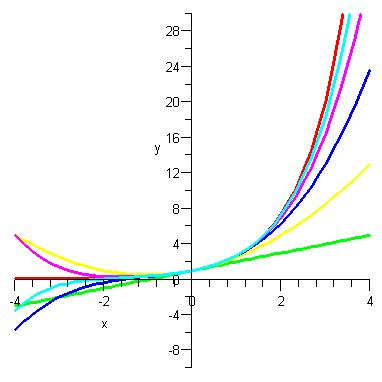
\includegraphics[width=\mywidth]{08-Power-Series/PowerSeries/taylore}&
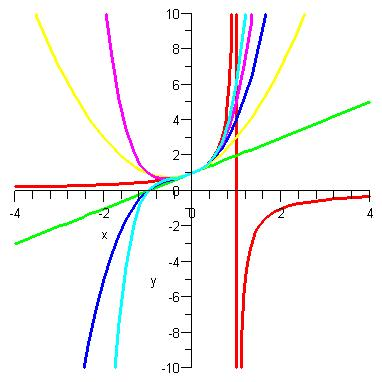
\includegraphics[width=\mywidth]{08-Power-Series/PowerSeries/taylor1}&
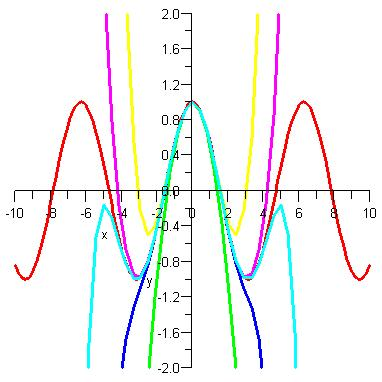
\includegraphics[width=\mywidth]{08-Power-Series/PowerSeries/taylorc}&
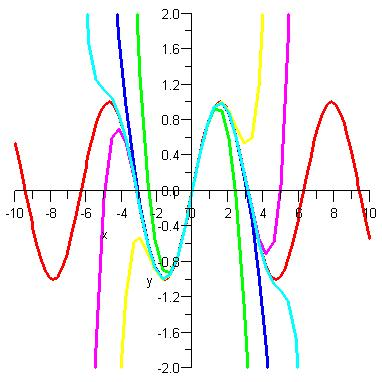
\includegraphics[width=\mywidth]{08-Power-Series/PowerSeries/taylors}
\\
$f(x)=e^x$&
$f(x)=\frac{1}{1-x}$&
$f(x)=\cos x$&
$f(x)=\sin x$
\end{tabular}
\end{center}
As you increase the degree of a Taylor polynomial, you should expect to see that your accuracy of approximating a function increases. This is true for $\cos x, \sin x, e^x,$ polynomials, and combination of these functions obtained through addition, subtraction, or multiplication. You can also divide any two of these function and still obtain good approximations, but vertical asymptotes pose a problem. 

The function $\frac{1}{1-x}$ has a vertical asymptote at $x=1$.  When we create Taylor polynomials centered at $x=0$, those polynomials follow the function up the left hand side of the vertical asymptote, causing the polynomials to tend toward infinity at $x=1$ as you increase the degree of the polynomial.  In the picture above, none of the polynomials do a good job of approximating the function to the right of $x=1$. Also, none of the functions do a good job of approximating the function to the left of $x=-1$. This is because Taylor polynomials are symmetric about where they are centered. When approximations break down on one side, they break down on the other side as well. We can only obtain useful approximations of $1/(1-x)$ for values of $x$ in the interval $(-1,1)$. The center of this interval is $x=0$, where we centered our Taylor polynomial. The distance from the center $x=0$ to the asymptote at $x=1$ is called our radius of convergence, and the interval of convergence $(-1,1)$ is obtained by moving 1 unit (the radius) to the right and left of 0 (the center).

%What happens if we change where we center our Taylor polynomial? When creating Taylor polynomials of increasing degree for $f(x) = 1/(1-x)$ centered at $x=-2$, the polynomials will do a great job of approximating the function until it reaches the asymptote at $x=1$.  Since the asymptote is 3 units away from $x=-2$ (where we centered the polynomial), our Taylor polynomials will produce increasing better approximations for any value of $x$ which is less than 3 units from $-2$, namely any $x$ in the interval $(-5,1)$. The number $3$ is our radius of convergence, and the interval $(-5,1)$ is our interval of convergence.
%
%There are vertical asymptotes for $\frac{1}{(x+4)(x-5)}$ at $-4$ and $5$. Taylor polynomials centered at $x=3$ produce useful approximations on an interval of radius 2 (the closer asymptote is at $x=5$ which is 2 units away), which means that as long as $x$ is in the interval $(1,5)$, you can use increasing larger Taylor polynomials centered at $x=3$ to make approximations good approximations. If instead you center the polynomials at $x=-1$, then the closest asymptote is at $x=-4$. This means the radius is $3$ and approximations can be made on the interval $(-4,2)$.  
%
%In math 316 you will learn about infinite sums of polynomials, and learn how to compute the radius of convergence using a tool called the ratio test. Taylor polynomials sometimes provide the only method known to numerically handle functions which are not polynomials (or quotients of polynomials). 





\subsection{Radius of convergence}
The Taylor series of a function involves adding infinitely many terms.  In some cases, the infinite sum will converge to a finite number. In other cases, the infinite sum will diverge. As an example, the Taylor series for $f(x) = \frac{1}{1-x}$ is $\ds  \sum_{m=0}^\infty x^m$. If $x=\frac{1}{2}$, then the series becomes $1+\frac{1}{2}+\frac{1}{4}+\frac{1}{8}+\frac{1}{16}+\cdots=2 = \frac{1}{1-1/2}$. We say this infinite sum converges to 2 because it gets closer and closer to 2 as you add more and more terms. Notice that the Taylor series actually converges to value of the function at $x=\frac{1}{2}$.  However, if you let $x=3$, then the series is $1+3+9+27+81+\cdots$ which diverges. In general, if a Taylor series converges at $x=c$, it will converge to $f(c)$. For this reason, we often write $\frac{1}{1-x} = \sum_{m=0}^\infty x^m$, and put an equal sign between the function and it's Taylor series.  However this equality sign will only hold if the series on the right converges. The infinite sum $\sum_{m=0}^\infty x^m$ is very closely related to the improper integral $\int_0^\infty x^m dm = \frac{x^m}{\ln x}\big|_{m=1}^\infty = \lim_{b\to\infty}\frac{x^b}{\ln x} - \frac{1}{\ln x}$. This improper integral converges if $0\leq x\leq 1$, and diverges otherwise. This integration fact can be used to show that sums of integer powers of $x$ converge if $|x|\leq 1$, and diverge if $|x|\geq 1$. We will use this fact to develop a powerful test called the ratio test which allows us to tell for which $x$ a power series will converge. 

For a series $\sum_{m=0}^\infty b_m$, the limit $\ds r=\lim_{m\to\infty}\frac{|b_{m+1}|}{|b_m|}$ compares how quickly a series grows.  Provided the limit $r$ exists, the series is comparable in growth to the series $\sum_{m=0}^\infty r^m$ which converges if $r\leq 1$ and diverges if $r>1$. A careful detailed analysis of this idea would require us to learn the Integral Test, absolute convergence, and comparison tests for series.  For our class, we will just use the fact that if $r<1$, then a series converges. For a Taylor series $\sum_{m=0}^\infty a_m (x-x_0)^m$ to converge, we need to satisfy the inequality $\lim_{m\to\infty}\frac{|a_{m+1}(x-x_0)^{m+1}|}{|a_m (x-x_0)^m|}<1$, or $\lim_{m\to\infty}\frac{|a_{m+1}|}{|a_m|}|x-x_0|<1$, or $|x-x_0|<1/ \lim_{m\to\infty}\frac{|a_{m+1}|}{|a_m|}$. We call the quantity $R=1/ \lim_{m\to\infty}\frac{|a_{m+1}|}{|a_m|}$ the radius of convergence of the power series because for $|x-x_0|<R$ the series converges. This formula for radius of convergence is handy if the series does not skip powers of $x$, however we return to the limit $\ds r=\lim_{m\to\infty}\frac{|b_{m+1}|}{|b_m|}<1$ to find the radius of convergence if the power series skips powers of $x$. In any case, a power series will have one of these three possible cases for it's radius of convergence: (1) $R=0$, so that the series only converges if $x=x_0$, (2) $R=\infty$, so that the series converges for all $x$ which is extremely nice, or (3) $R>0$, so that the series converges for $|x-x_0|<R$.

The series $\frac{1}{1-x}= \sum_{m=0}^\infty x^m$ has radius of convergence $\ds R=1/\lim_{m\to\infty}\frac{|1|}{|1|} = 1$, so if $|x|<1$ the series converges.  For the function $e^x = \sum_{m=0}^\infty \frac{x^m}{m!}$, the radius of convergence is $\ds R=1/\lim_{m\to\infty}\frac{|1/(m+1)!|}{|1/m!|} =1/\lim_{m\to\infty}\frac{m}{m+1} =\infty$ which means that the Taylor series for $e^x$ converges for all $x$. We have the series $\cos x = \sum_{m=0}^\infty \frac{1}{(2m)!} x^{2m}$ which skips powers of $x$.  Hence we solve $\ds \lim_{m\to\infty}\frac{|x^{2(m+1)}/(2(m+1))!|}{| x^{2m}/(2m)!|}<1$ which is equivalent to $|x^2|\lim_{m\to\infty}\frac{(2m)!}{ (2m+2)(2m+1)(2m)!}<1$ or $0<1$ which is always true so the radius of convergence is $\infty$ and the Taylor series converges for all $x$.  You should show that this is true for $\sin x$ as well. 

Let's find the radius of convergence of the power series $\ds\sum_{n=0}^\infty \frac{(3n+2)(-5)^n}{(n+1)(7n^2+3)2^{3n+1}}x^{2n}$.  We compute $a_{n+1} = \frac{(3(n+1)+2)(-5)^{n+1}}{((n+1)+1)(7(n+1)^2+3)2^{3(n+1)+1}}x^{2(n+1)}$.  Dividing by $a_n$ can get ugly unless we organize our work, for example by placing common terms directly above and below each other as shown below.
\begin{align*}
\left|\frac{a_{n+1}}{a_n}\right| 
&=  
\left|\begin{array}{c|c|c|c|c|c}
(3(n+1)+2)&(-5)^{n+1}&(n+1)&(7n^2+3)&2^{3n+1}&x^{2(n+1)}\\\hline
(3n+2)&(-5)^n&((n+1)+1)&(7(n+1)^2+3)&2^{3(n+1)+1}&x^{2n}
\end{array}\right|\\
&=\left|\begin{array}{c|c|c|c|c|c}
(3n+5)&(-5)^{n}(-5)&(n+1)&(7n^2+3)&2^{3n}2&x^{2n}x^2\\\hline
(3n+2)&(-5)^n&(n+2)&(7(n+1)^2+3)&2^{3n}2^{4}&x^{2n}
\end{array}\right|\\
&=\left|\begin{array}{c|c|c|c|c|c}
(3n+5)&(-5)&(n+1)&(7n^2+3)&1&x^2\\\hline
(3n+2)&1&(n+2)&(7(n+1)^2+3)&2^{3}&1
\end{array}\right|
\end{align*}
Recall that the limit of a product can be found by computing each individual limit and the multiplying the result together.  Also, the limit as $n\to \infty$ of a quotient of two polynomials of the same degree is precisely the quotient of their leading coefficients.  This means we can compute 
$\ds\lim_{n\to\infty}\frac{(3n+5)}{(3n+2)} = 1 $, 
$\ds\lim_{n\to\infty}\frac{(n+1)}{(n+2)} = 1 $, and 
$\ds\lim_{n\to\infty}\frac{(7n^2+3)}{(7(n+1)^2+3)} = 1$, which gives 
$$\lim_{n\to\infty}
\left|\begin{array}{c|c|c|c|c|c}
(3n+5)&(-5)&(n+1)&(7n^2+3)&1&x^2\\\hline
(3n+2)&1&(n+2)&(7(n+1)^2+3)&2^{3}&1
\end{array}\right| = \left|1(-5)(1)(1)\left(\frac{1}{8}\right)x^2\right| = \frac{5}{8}x^2.$$ 
We then solve the equation $\frac{5}{8}x^2<1$ for $x$ to obtain $|x|\leq\sqrt{\frac{8}{5}}$, so the radius of convergence is $\sqrt{\frac{8}{5}}$.

\subsection{Euler's Formula}
We now show $e^{ix}=\cos x+i\sin x$.  We know $\ds e^x = \sum_{m=0}^\infty\frac{1}{m!}x^m$ for all $x$, and it can be shown that this formula is valid as well for all complex numbers.  If we replace $x$ with $ix$, then we obtain $\ds e^{ix} = \sum_{m=0}^\infty\frac{1}{m!}(ix)^m$.  The powers of $i$ satisfy $i^0=1, i^1=i, i^2=-1, i^3=-i, i^4=1, i^5=i$, and cycle through the numbers $1,i,-1,-i$.  Hence we have for all $x$ Euler's formula
\begin{align*}
e^{ix} 
&= 1+ix-\frac{1}{2!}x^2-i\frac{1}{3!}x^3+\frac{1}{4!}x^4+i\frac{1}{5!}x^5-\frac{1}{6!}x^6-i\frac{1}{7!}x^7+\cdots\\
&= \left(1-\frac{1}{2!}x^2+\frac{1}{4!}x^4-\frac{1}{6!}x^6+\cdots\right)
+i\left(x-\frac{1}{3!}x^3+\frac{1}{5!}x^5-\frac{1}{7!}x^7+\cdots\right)\\
&= \left(\sum_{m=0}^\infty \frac{(-1)^m}{(2m)!}x^{2m}\right)
+i\left(\sum_{m=0}^\infty \frac{(-1)^m}{(2m+1)!}x^{2m+1}\right)\\
&= \cos(x)+i\sin(x).
\end{align*} 
%This means that $e^{(\alpha+\beta i)x} = e^{\alpha x}e^{\beta x i} = e^{\alpha x}(\cos\beta x +i\sin\beta x)$. This is Euler's formula. 

Who cares?  Well, if the roots of the second order ODE $my^{\prime\prime}+cy^\prime+ky=0$ are complex, i.e. $\lambda=a\pm b i$, then $y_1=e^{a x+ b ix} =e^{a x}(\cos b x+ i\sin b x)$ and $y_2=e^{a x-b i x}=e^{a x}(\cos (-bx)+i\sin(-b x)) = e^{a x}(\cos b x-i\sin b x)$ are two complex solutions of the ODE (recall that $\cos (-x)=\cos (x)$ [cosine is an even function] and $\sin(-x)=-\sin x$ [sine is an odd function]). The superposition principle for ODEs says that linear combinations are solutions, so $\frac{y_1+y_2}{2} = e^{a x}\cos b x$ and $\frac{y_1-y_2}{2i} = e^{a x}\sin b x$ are two real solutions.  This is why we use $e^{a x}\cos b x$ and $e^{a x}\sin b x$ as solutions when the roots of the characteristic equation are imaginary.

\section{Power Series}
\subsection{Notation and Calculus}
Rather than starting with a function $f(x)$ and calculating the Taylor series, we now reverse the process.  We will define a power series centered at $x=c$ to be an expression of the form $f(x) = \sum_{m=0}a_m (x-c)^m$, and the domain of $f$ is all $x$ for which the series converges. We will almost always center our power series at $x=0$, so we write $f(x) = \sum_{m=0}a_m x^m$. The radius of convergence is still computed the same. 
If the power series has a positive or infinite radius of convergence when centered at $x=c$, then we say that the function $f(x)= \sum_{m=0}a_m (x-x_0)^m$ is \textbf{analytic} at $c$. 

If a power series $f(x)= \sum_{m=0}a_m (x-x_0)^m$ has a finite radius of convergence, then we can differentiate and integrate the power series term by term. The resulting power series $f^\prime (x) = \sum_{m=0}m a_m (x-x_0)^{m-1}=\sum_{m=1}m a_m (x-x_0)^{m-1} $ and $\int f(x)dx = C+\sum_{m=0}\frac{a_m}{m+1} (x-x_0)^{m+1}$ have the same radius of convergence as $f$.  If two power series centered at the same point both converge at $x$, then you can add them (by adding their coefficients), and multiply them (using the distributive laws of multiplication). In addition, you can compose power series, though this may change the radius of convergence.  The most common composition is to replace $x$ with $a(x)^k$ for some constants $a$ and $k$. 

\subsection{Examples}
Since $\ds \frac{1}{1-x} = \sum_{m=0}^\infty x^m$ has radius of convergence $R=1$, we can differentiate and obtain $\ds \frac{1}{(1-x)^2} = \sum_{m=1}^\infty m x^{m-1} = 1+2x+3x^2+4x^3+\cdots$, which has radius of convergence $R=1$ as well.  Replacing $x$ with $x=-x$ gives $\ds \frac{1}{1+x} = \sum_{m=0}^\infty (-1)^m x^m = 1-x+x^2-x^3+x^4+\cdots$. Replacing $x$ with $-x^2$ gives $\ds \frac{1}{1+x^2} = \sum_{m=0}^\infty (-1)^m x^{2m} = 1-x^2+x^4-x^6+x^8+\cdots$. Integration of $\frac{1}{1+x^2}$ gives (notice that $\arctan(0)=0$ so the constant is zero) $\arctan x = \ds \sum_{m=0}^\infty \frac{(-1)^m}{2m+1} x^{2m+1} = x-\frac13x^3+\frac15x^5-\frac17x^7+\frac19x^9+\cdots$, with radius of convergence $R=1$. For homework, find the power series of $\ln|1+x|,\ln\left|\frac{1+x}{1-x}\right|,\frac{x}{1+x^2},$ and a few others that you can find any any calculus textbook.  

To find the radius of convergence of the power series $\arctan 2x = \ds \sum_{m=0}^\infty \frac{(-1)^m}{2m+1} (2x)^{2m+1}$, we notice that powers of $x$ are skipped. So we solve 
$\ds \lim_{m\to\infty}\frac{|(2x)^{2(m+1)+1}/(2(m+1)+1)|}{|(2x)^{2m+1}/2m+1|}<1$, 
which is equivalent to 
$\ds \lim_{m\to\infty}\frac{(2x)^{2m+3}(2m+1)}{(2x)^{2m+1}(2m+3)}<1$ or
$\ds (2x)^2 \lim_{m\to\infty}\frac{(2m+1)}{(2m+3)}<1$. Taking limits gives $(2x)^2<1$ or $|2x|<1$ which means $|x|<\frac{1}{2}$. Hence the radius of convergence is 1/2.  

The radius of convergence of the power series $f(x) = \sum_{m=0}\frac{m}{8^m} x^{3m}$ can be found by solving 
$\ds \lim_{m\to\infty}\frac{|(m+1)x^{3(m+1)}/8^{m+1}|}{|mx^{3m}/8^{m}|}<1$. The left side simplifies as 
$\ds \lim_{m\to\infty}\frac{(m+1)x^{3m+3)}/8^{m}8}{mx^{3m}/8^{m}} = |x^3|\lim_{m\to\infty}\frac{(m+1)/8}{m} =|x^3/8|$.  The solution to $|x^3/8|<1$ is $|x^3|<8$ or $|x|<2$.  Hence the radius of convergence is $2$. Notice that we know this power series converges for $|x|<2$, even though we do not know what it converges to.   

\subsection{Shifting Indices}
Often we will find it necessary to shift the indices of a power series. The series $\ds\sum_{m=1}^\infty m a_m x^{m-1}$ is equivalent (letting $s=m-1$ or $m=s+1$) to the series $\ds\sum_{s=0}^\infty (s+1)a_{s+1} x^{s}$. The variables $m$ and $s$ are just ``dummy'' variables used as a place holder.  They can be changed as much as you want, just as you can change the variable of integration in an integration problem.  The change $s=m-1$ is called shifting the indices of a series.  The series $\ds\sum_{m=3}^\infty \frac{m+1}{m-2} x^{m-3}$ can be shifted to start at $0$ by letting $s=m-3$, and then we write $\ds\sum_{s=0}^\infty \frac{s+4}{s+1} x^{s}$, since $m=s+3$ (just replace each $m$ with $s+3$ and the result follows). 












\section{Series Solutions to ODEs}


Recall that a function which can be represented by a power series centered at $c$ with a positive radius of convergence is said to be analytic at $c$. It can be shown that the 2nd order ODE $h(x)y^{\prime\prime}+p(x)y^\prime+q(x)y=r(x)$ has a power series solution centered at $c$ if $h,p,q,r$ are all analytic at $c$ and $h(x_0)\neq 0$. Alternatively, if we divide by $h(x)$, then the 2nd order ODE $y^{\prime\prime}+a(x)y^\prime+b(x)y=c(x)$ has a power series solution centered at $x=c$ if $a(x),b(x),c(x)$ are all analytic at $x=c$.  In this case we call $x=c$ an ordinary point of the ODE.  The radius of convergence of the power series solution we obtain for $y(x)$ will be at least as big as the smallest radius of convergence of $a(x),b(x),c(x)$. This is the general theory which motivates everything else we do with regards to series solutions to ODEs. 

The power series method essentially requires that you (1) write $\ds y=\sum_{n=0}^\infty a_n x^n$, (2) take derivatives $\ds y=\sum_{n=0}^\infty n a_n x^{n-1}$ and $\ds y=\sum_{n=0}^\infty n(n-1) a_n x^{n-2}$, (3) replace each function or derivative in your ODE with the appropriate power series (computing MacLaurin series of functions which occur) (4) shift the indices on each sum to obtain a recurrence relation for the unknown constants $a_n$, and then (5) solve the recurrence relation for the largest $a_n$ and use this relation to generate the constants.  The following 4 examples illustrate how to find solutions using the power series method. Some of these problems you already can solve without power series methods, however we will start with simpler problems to which you already know the answer before we venture into new problems.

Consider the ODE $y^\prime=ky$.  Let $\ds y=\sum_{m=0}^\infty a_m x^m$.  Then we compute
$\ds y^\prime 
= \sum_{m=0}^\infty m a_m x^{m-1} 
= \sum_{m=1}^\infty m a_m x^{m-1} 
$. Notice that we can start at $m=1$ instead of $m=0$ because when you put $m=0$ into the sum you get zero, so why not just start one term later and skip the 0 term.
Inserting these series into the ODE gives 
$\ds \sum_{m=1}^\infty m a_m x^{m-1}=k\sum_{m=0}^\infty a_m x^m = \sum_{m=0}^\infty ka_m x^m$. For this equality to hold, we must have the coefficient of each power $x$ equal on each side of the equation.  To simplify the calculations, we shift the indices on the power series on the left by letting $m-1=s$, and on the right by letting $m=s$.  This gives $\ds \sum_{s=0}^\infty (s+1) a_{s+1} x^{s}= \sum_{s=0}^\infty ka_s x^s$, which means that $(s+1) a_{s+1} = ka_s$ for all $s$.  This gives the recurrence relation $a_{s+1}=\frac{ka_s}{(s+1)}$.  The variable $a_0$ can be chosen to be anything we want, but then $a_1=\frac{ka_0}{1},a_2=\frac{k^2a_0}{2!},a_3=\frac{k^3a_0}{3!}, a_m=\frac{k^ma_0}{m!}$.  So we have our solution as $$y(x) = a_0+a_0\frac{k}{1!}x^1+a_0\frac{k^2}{2!}x^2+\cdots = a_0\left(1+\frac{1}{1!}(kx)^1 + \frac{1}{2!}(kx)^2+\cdots\right) = a_0 \sum_{m=0}^\infty \frac{1}{m!}(kx)^m= a_0 e^{kx},$$ where the last equality comes because we recognize that this is the Maclaurin series of $e^{kx}$.

Consider the ODE $y^\prime=xy$. Let $\ds y=\sum_{m=0}^\infty a_m x^m$.  Then we compute
$\ds y^\prime 
= \sum_{m=0}^\infty m a_m x^{m-1} 
= \sum_{m=1}^\infty m a_m x^{m-1} 
$ (again we start at 1 because $m=0$ just gives us zero).
Inserting these series into the ODE gives 
$\ds \sum_{m=1}^\infty m a_m x^{m-1}=x\sum_{m=0}^\infty a_m x^m = \sum_{m=0}^\infty a_m x^{m+1}$.
Writing out the first few terms, we have $$1a_1x^0+2a_2x^1+3a_3x^2+4a_4x^3+\cdots = a_0x^1+a_1x^2+a_2x^3+a_3x^4.$$
Since $x^0$ appears only on the left side of the equation, we have $a_1=0$.  Hence the left side can be written $\ds \sum_{m=2}^\infty m a_m x^{m-1}$. We shift indices by letting $s=m-1$ ($m=s+1$) on the left side and $s=m+1$ on the right side.  This gives 
$\ds \sum_{s=1}^\infty (s+1) a_{s+1} x^{s}=\sum_{s=1}^\infty a_{s-1} x^{s}$. Equating the coefficients of $x^s$ (for $s\geq 1$) gives $(s+1) a_{s+1} = a_{s-1}$, or $a_{s+1} = \frac{a_{s-1}}{(s+1)}$ for $s\geq 1$.  For $s=1,2,3,4,5,6,\ldots$ we have $a_{2} = \frac{a_{0}}{(2)},a_{3} = \frac{a_{1}}{(3)}=0, a_{4} = \frac{a_{2}}{(4)} =\frac{a_{0}}{(2\cdot 4)}, a_5=0, a_6=\frac{a_{0}}{(2\cdot 4\cdot 6)} = \frac{a_{0}}{2^3 3!}, \ldots$.  Notice that $a_m=0$ for odd $m$, and $a_{2m}=\frac{a_{0}}{2^m m!}$.  If $m=0$, we can still write $a_{2m}=\frac{a_{0}}{2^m, m!}=a_0$, which means we can write $y=\sum_{m=0}^\infty \frac{a_{0}}{2^m m!}x^{2m} = a_0\sum_{m=0}^\infty \frac{1}{m!}\left(\frac{x^2}{2}\right)^{m} = a_0e^{x^2/2}$.


Now consider the ODE $y^{\prime\prime}+y=0$.  Let $\ds y=\sum_{m=0}^\infty a_m x^m$.  Then we compute 
$\ds y^\prime 
= \sum_{m=0}^\infty m a_m x^{m-1} 
= \sum_{m=1}^\infty m a_m x^{m-1} 
$ and 
$\ds y^{\prime \prime }
= \sum_{m=1}^\infty m(m-1) a_m x^{m-2} 
= \sum_{m=2}^\infty m(m-1) a_m x^{m-2} 
$ (we can start the second derivative at $m=2$ because putting $m=0$ or $m=1$ into the series gives 0).
Inserting these power series into the ODE gives $\sum_{m=2}^\infty m(m-1) a_m x^{m-2}+\sum_{m=0}^\infty a_m x^m=0$.  Shifting the indices on the first sum using $s=m-2$ (or $m=s+2$) and second sum using $m=s$ gives $\sum_{s=0}^\infty (s+2)(s+1) a_{s+2} x^{s}+\sum_{s=0}^\infty a_s x^s=0$. We need to have the sum of the coefficients of $x^s$ sum to zero, so we have $(s+2)(s+1) a_{s+2} + a_s=0$.  This means $a_{s+2} = -\frac{a_s}{(s+2)(s+1)}$ for $s\geq 0$.  This recurrence relation does not specify $a_0$ or $a_1$, so we have two constants we can choose arbitrarily.  For $s=0,1,2,3,\ldots$, we have $a_{2} = -\frac{a_0}{2!}, a_{3} = -\frac{a_1}{3!},a_{4} = \frac{a_0}{4!},a_{5} = \frac{a_1}{5!},a_{6} = -\frac{a_0}{6!},a_{7} = -\frac{a_1}{7!}\ldots$. The sign changes in groups of two, which suggests we should split the series into even and odd powers. This can be summarized as $a_{2m}=(-1)^m\frac{a_0}{(2m)!}$ and $a_{2m+1}=(-1)^m\frac{a_1}{(2m+1)!}$.  This means that the solution to the ODE is 
\begin{align*}
y(x) &= a_0+a_1x-a_0\frac{1}{2!}x^2-a_1\frac{1}{3!}x^3+a_0\frac{1}{4!}x^4+a_1\frac{1}{5!}x^5+\cdots \\
&=a_0\left(1-\frac{1}{2!}x^2+\frac{1}{4!}x^4+\cdots\right)+a_1\left(x-\frac{1}{3!}x^3+\frac{1}{5!}x^5+\cdots\right)\\
&= a_0\left(\sum_{m=0}^\infty \frac{(-1)^m}{(2m)!}x^{2m}\right)+a_1\left(\sum_{m=0}^\infty \frac{(-1)^m}{(2m+1)!}x^{2m+1}\right)\\
&= a_0\cos(x)+a_1\sin(x).\\
\end{align*}
The last equality can be discovered by recognizing that the series are the MacLaurin series for cosine and sine.


As our last example, consider the ODE
$y^{\prime\prime}+2xy^\prime+y=0$. Let $\ds y=\sum_{m=0}^\infty a_m x^m$. Then we compute 
$\ds y^\prime 
= \sum_{m=0}^\infty m a_m x^{m-1} 
= \sum_{m=1}^\infty m a_m x^{m-1} 
$ and 
$\ds y^{\prime \prime }
= \sum_{m=1}^\infty m(m-1) a_m x^{m-2} 
= \sum_{m=2}^\infty m(m-1) a_m x^{m-2} 
$.
Inserting these power series into the ODE and multiplying the middle series by 2x gives 
$$\sum_{m=2}^\infty m(m-1) a_m x^{m-2}+\sum_{m=1}^\infty 2m a_m x^{m} +y=\sum_{m=0}^\infty a_m x^m=0.$$ We shift the index on the first series by letting $s=m-2$ and $s=m$ for the last two.  This gives 
$$\sum_{s=0}^\infty (s+2)(s+1) a_{s+2} x^{s}+\sum_{s=1}^\infty 2s a_s x^{s} +\sum_{s=0}^\infty a_s x^s=0.$$ Notice that the second series starts at $s=1$ whereas the other two start at $s=0$.  Hence we look at the coefficients of $x^0$ separately than the rest of the coefficients.  We notice that $(2)(1)a_2 +a_0 = 0$, or $a_2=-a_0\frac{1}{2!}$.  For $s\geq 1$ we have $(s+2)(s+1) a_{s+2}+2s a_s+a_s =0$, or $ a_{s+2} = -a_s\frac{2s+1}{(s+2)(s+1)}$. The first few terms are $a_2=-a_0\frac{1}{2!}, a_3 = -a_s\frac{3}{(3)(2)}, a_4=a_0\frac{1\cdot 5}{4!},a_5=a_1\frac{3\cdot 7}{5!},a_6=-a_0\frac{1\cdot 5\cdot 9}{6!},-a_7=a_1\frac{3\cdot 7\cdot 11}{7!}$. Since the even and odd coefficients $a_m$ depend on $a_0$ and $a_1$, we write $a_{2m}=a_0(-1)^m \frac{1\cdot 5\cdot 9\cdots(4m-3)}{(2m)!}$ and $a_{2m+1}=a_1(-1)^m\frac{3\cdot 7\cdot 11\cdots(4m-1)}{(2m+1)!}$. Hence we have found a solution as 
\begin{align*}
y(x) &= a_0\left(1-{\frac {1}{2}}{t}^{2}+{\frac {5}{24}}{t}^{4}-{
\frac {1}{16}}{t}^{6}+{\frac {13}{896}}{t}^{8}+\cdots
 \right) +a_1\left(t-{\frac {1}{2}}{t}^{3}+{\frac {7}{40}}{t}^{5}-{
\frac {11}{240}}{t}^{7}+{\frac {11}{1152}}{t}^{9} +\cdots\right)\\
&= a_0\left(1+\sum_{m=1}^\infty (-1)^m \frac{1\cdot 5\cdot 9\cdots(4m-3)}{(2m)!}x^{2m} \right) +a_1\left(x+\sum_{m=1}^\infty (-1)^m\frac{3\cdot 7\cdot 11\cdots(4m-1)}{(2m+1)!}x^{2m+1} \right). 
\end{align*}
This is not a simple elementary function for which we know a power series. The radius of convergence is $R=\infty$.  We will learn how to express this function in terms of Bessel functions and Gamma functions when we start studying special functions in the next learning module.  Hence, we leave our solution in terms of a power series and cannot continue any further.

As you work problems in the homework, I want you to find general formulas for the $m$th coefficient $a_m$. Mathematica has code you can use to check if your answers are correct, as well as show you many of the steps in the computation. 


\newgeometry{left=1in,right=1in,top=1in,bottom=1in}

\section{Preparation}

\noindent  
This chapter covers the following ideas. When you create your lesson plan, it should contain examples which illustrate these key ideas. Before you take the quiz on this unit, meet with another student out of class and teach each other from the examples on your lesson plan. 


\begin{enumerate}
\item Find and explain the use of Taylor polynomials, Talyor series, and Maclaurin series. Give examples for various common functions.
\item Explain how to use the ratio test to find the radius of convergence of a power series. 
\item Derive Euler's formula, and use it to explain why complex roots $a\pm bi$ of 2nd order ODE result in the solutions $e^{ax}\cos(bx)$ and $e^{ax}\sin(bx)$.
\item Explain how to differentiate, integrate, add, multiply, compose, and shift indices of power series.
\item Use the power series method to solve ODEs at ordinary points.
\end{enumerate}



Here are the preparation problems for this unit. Chapter numbers precede the problems from Schaum's.
\begin{center}
\begin{tabular}{ll}
&Preparation Problems 
(\href{https://ilearn.byui.edu/bbcswebdav/institution/Physical\_Sci\_Eng/Mathematics/Personal\%20Folders/WoodruffB/316/08-Power-Series-Preparation-Solutions.pdf}{click for solutions})
\\
\hline\hline
Day 1& 1, 11, 18, 20
\\\hline
Day 2& 25, 29, 43, Schaum's 27:3
\\\hline
Day 3& 46, Schaum's 27:29, Schaum's 27:36, Schaum's 27:41
\\\hline
\end{tabular}
\end{center}


The homework for this unit comes from the Power Series chapter in this online book.  Please make sure you print the appropriate pages from the problem book, as well as the corresponding section from the textbook.  

Make sure you try a few of each type of problem, ASAP. I suggest that the first night you try one of each type of problem. It's OK if you get stuck and don't know what to do, as long as you decide to learn how to do it and then return to the ones where you got stuck. Eventually do enough of each type to master the ideas.  The only section in Schaum's with relevant problems is chapter 27.  

Most engineering textbooks assume you have seen Taylor series and power series before (in math 113), but many of you have not. If you have your old Math 215 book, you can find many relevant problems and explanations from section 11.5 (Ratio Test) and 11.8 (Taylor Series).  

For reference, here are a few key functions and their Taylor series centered at $x=0$ (so their MacLaurin series).

\begin{enumerate}
	\item $\ds e^x = \sum_{n=0}^\infty \frac{1}{n!}x^n$, $R=\infty$
	\item $\ds \cos(x) = \sum_{n=0}^\infty \frac{(-1)^n}{(2n)!}x^{2n}$, $R=\infty$
	\item $\ds \sin(x) = \sum_{n=0}^\infty \frac{(-1)^n}{(2n+1)!}x^{2n+1}$, $R=\infty$
	\item $\ds \frac{1}{1-x} = \sum_{n=0}^\infty x^n$, $R=1$
	\item $\ds \cosh(x) = \sum_{n=0}^\infty \frac{1}{(2n)!}x^{2n}$, $R=\infty$
	\item $\ds \sinh(x) = \sum_{n=0}^\infty \frac{1}{(2n+1)!}x^{2n+1}$, $R=\infty$
\end{enumerate}

\section{Problems}

\begin{multicols}{2}

\begin{enumerate}

\item [(I)] For each of the following, find a Talyor polynomial of degree $n$ centered at $x=c$ of the function $f(x)$.
\begin{multicols}{2}
\item $e^{4x}, n=3, c=0$
\item $\cos(x), n=4, c=\pi$
\item $\cos(2x), n=4, c=0$
\item $\sin(\frac12 x), n=5, c=0$
\item $\frac{1}{x}, n=3, c=1$
\item $\ln x, n=3, c=1$
\item $\ln (1-x), n=4, c=0$
\item $\ln (1+x), n=4, c=0$
\end{multicols}






\item [(II)] Find the radius of convergence of each power series.
\begin{multicols}{2}
\item $\ds \sum_{n=0}^\infty \frac{1}{3^n}x^n$
\item $\ds \sum_{n=0}^\infty \frac{(-1)^n}{4^{n+1}}x^{n}$
\item $\ds \sum_{n=0}^\infty \frac{n}{2^n}x^{3n}$
\item $\ds \sum_{n=0}^\infty \frac{3n+1}{n^2+4}x^n$
\item $\ds \sum_{n=0}^\infty \frac{(-4)^n n}{n^2+1}x^{2n}$
\item $\ds \sum_{n=0}^\infty \frac{n}{2^n}x^{2n}$
\item $\ds \sum_{n=0}^\infty \frac{(-1)^n}{n!}x^{n}$
\item $\ds \sum_{n=0}^\infty \frac{n!}{10^n}x^{2n}$
\end{multicols}





\item [(III)] For each function, find the MacLaurin series and state the radius of convergence.
\begin{multicols}{2}
\item $f(x)=e^x$
\item $f(x)=\cos x$
\item $f(x)=\sin x$
\item $\ds f(x)=\frac{1}{1-x}$
\item $\ds f(x)=\frac{1}{1+x}$
\item $f(x)=\cosh x$
\item $f(x)=\sinh x$
\end{multicols}






\item [(IV)] Prove the following formulas are true by considering power series. These formulas will allow us to eliminate complex numbers in future sections.
\item $e^{ix}=\cos x + i\sin x$ (called Euler's formula)
\begin{multicols}{2}
\item $\cosh(ix) = \cos x$
\item $\cos(ix) = \cosh x$
\item $\sinh(ix) = i\sin x$
\item $\sin(ix) = i\sinh x$
\end{multicols}







\item [(V)] Use MacLaurin series of known functions to find the MacLaurin series of these functions (by integrating, differentiating, composing, or multiplying together two power series). Then state the radius of convergence.
\item $f(x)={x^2}{e^{3x}}$
\item $f(x)=\frac{x^2}{e^{3x}}$ [hint, use negative exponents]
\item $f(x)=\cos 4x$
\item $f(x)=x\sin(2x)$ 
\item $f(x)=\frac{x}{1+x}$
\item $f(x)=\frac{1}{1+x^2}$
\item $f(x)=\arctan x$ [hint, integrate the previous]
\item $f(x)=\arctan (3x)$ 





\item [(VI)] Shift the indices on each sum so that it begins at $n=0$.
\begin{multicols}{2}
\item $\ds\sum_{n=3}^6 n+2$ 
\item $\ds\sum_{n=2}^8 n^2$ 
\item $\ds\sum_{n=4}^\infty 2^n$ 
\item $\ds\sum_{n=2}^\infty x^n$ 
\item $\ds\sum_{n=1}^\infty n a_n x^{n}$ 
\item $\ds\sum_{n=2}^\infty n (n-1) a_n x^{n-2}$ 
\end{multicols}






\item [(VII)] Solve the following ODEs by the power series method. With some, initial conditions are given (meaning you know $y(0)=a_0$ and $y^\prime(0)=a_1$). Identify the function whose MacLaurin series equals the power series you obtain.
\item $y^{\prime}=3y$
\item $y^{\prime}=2xy$
\item $y^{\prime\prime}+4y=0$
\item $y^{\prime\prime}-9y=0, y(0)=2, y^\prime(0)=3$
\item $y^{\prime\prime}+4y^{\prime}+3y=0, y(0)=1, y^\prime(0)=-1$



\item [(VII)] Determine whether the given values of $x$ are ordinary points or singular points of the given ODE.
\item Chapter 27, problems 26-34 (these are really quick).


\item [(VIII)] Solve the following ODEs by the power series method.  State the recurrence relation used to generate the terms of your solution, and write out the first 5 nonzero terms of your solution.
\item Chapter 27, problems 35-47 (or from the worked problems).






\end{enumerate}

\section{Solutions}
Handwritten solutions are available online.  \href{https://ilearn.byui.edu/bbcswebdav/institution/Physical\_Sci\_Eng/Mathematics/Personal\%20Folders/WoodruffB/316/08-Power-Series-Preparation-Solutions.pdf}{Click for solutions.}

\end{multicols}



\restoregeometry



\chapter{Special Functions}

{This section needs revamping.  Until I have time to revamp it, Schaum's Outlines provides a great explanation of these topics. }


\noindent The name of this chapter is ``Special Functions.'' These are functions which show up as the solution to problems of real world interest whose solution is a function which does not appear in regular calculus.  Many of these functions can only be represented using series. This chapter covers the following objectives:


\begin{enumerate}
\item Explain the Frobenius method and use it to solve ODEs where zero is a regular singular point.
\item Solve Legendre's equation and derive Legendre polynomials.
\item Solve Bessel's equation giving solutions of the first kind, and write solutions to ODEs in terms of Bessel functions.
\item Describe the Gamma function and how it generalizes the factorial. Be able to prove various relationships related to the Gamma function.
\end{enumerate}



%
%When you make your lesson plan, it should explain and contain examples of the following:
%\begin{enumerate}
%\item Explain the Frobenius method and use it to solve ODEs where zero is a regular singular point.
%\item Solve Legendre's equation and derive Legendre polynomials.
%\item Solve Bessel's equation giving solutions of the first kind, and write solutions to ODEs in terms of Bessel functions.
%\item Describe the Gamma function and how it generalizes the factorial. Be able to prove various relationships related to the Gamma function.
%\end{enumerate}
%
%
%
%\section{Legendre's Equation}
%Legendre's equation is the ODE $(1-x^2)y^{\prime\prime}-2xy^\prime+n(n+1)y=0$. It appears in physics often and is used to solve problems which have radial symmetry.  We will solve this ODE in general, and then look at the special cases where $n$ is a positive integer value. Since $1-x^2\neq 0$ at $x=0$, and $-2x$ and $n(n+1)$ are analytic functions (meaning they can be represented using a power series with a positive radiu of convergence), this ODE has a power series solution.  Hence we let $\ds y=\sum_{m=0}^\infty a_mx^m, y^\prime=\sum_{m=1}^\infty ma_mx^{m-1}, y^{\prime\prime}=\sum_{m=2}^\infty m(m-1)a_mx^{m-2}$.  Inserting these into the ODE gives 
%\begin{align*}
%&\sum_{m=2}^\infty (1-x^2)m(m-1)a_mx^{m-2}
%-\sum_{m=1}^\infty 2xma_mx^{m-1}
%+\sum_{m=0}^\infty n(n+1)a_mx^m\\
%&=
%\sum_{m=2}^\infty m(m-1)a_mx^{m-2}-\sum_{m=2}^\infty m(m-1)a_mx^{m}
%-\sum_{m=1}^\infty 2ma_mx^{m}
%+\sum_{m=0}^\infty n(n+1)a_mx^m=0.
%\end{align*}
%Shifting indices on the first power series ($s=m-2$) gives 
%\begin{align*}
%\sum_{s=0}^\infty (s+2)(s+1)a_{s+2}x^{s}-\sum_{s=2}^\infty s(s-1)a_sx^{s}
%-\sum_{s=1}^\infty 2sa_sx^{s}
%+\sum_{s=0}^\infty n(n+1)a_sx^s=0.
%\end{align*}
%Since two series start at 0, one at 1, and one at 2, we write down the coefficients for the first two terms, giving $(2)(1)a_2+n(n+1)a_0=0$ and $(3)(2)a_3-2a_1+n(n+1)a_1=0$. Then the general recurrence relation is $$(s+2)(s+1)a_{s+2} - s(s-1)a_s-2sa_s+n(n+1)a_s,$$ or after solving for $a_{s+2}$ we obtain $$\ds a_{s+2} = \frac{s(s-1)+2s-n(n+1)}{(s+2)(s+1)} a_s= -\frac{(n-s)(n+s+1)}{(s+2)(s+1)}a_s$$ (the last equality is just a convenient way that someone discovered to rewrite the relation). Notice that if $s=0$ or $s=1$, this equation is also valid as the terms which do not appear in the first two equations become zero. We calculate the first few terms as $a_0=a_0, a_1=a_1, a_2 = -\frac{n(n+1)}{2!}a_0, a_3 = -\frac{(n-1)(n+2)}{3!}a_1, a_4 = -\frac{(n-2)(n+3)}{4\cdot 3}a_2 = \frac{(n-2)(n)(n+1)(n+3)}{4!}a_0, a_5 = -\frac{(n-3)(n+4)}{5\cdot 5}a_3 = \frac{(n-3)(n-1)(n+2)(n+4)}{4!}a_1,\ldots$. So using these coefficients we can write $y=a_0y_1+a_1y_2$ as the solution to Legendre's equation, where $y_1$ contains only even powers of $x$ and $y_2$ contains only odd powers of $x$.
%
%Notice that if $n$ is a positive integer, then $a_{n+2}=0$ means that $a_{n+2m}$ is zero for all $m\geq 1$ as the recursion looks at two terms back.  If $n$ is even, this means that the power series for $y_1$ will terminate and represent a polynomial.  Similarly, if $n$ is odd, then the coefficients of $y_2$ will terminate.  Hence for any positive integer $n$, one of the solutions is a polynomial, which we will call $P_n(x)$. To remove the arbitrary coefficient $a_0$ or $a_1$ from the solution, we choose $a_n=\frac{(2n)!}{2^n(n!)^2}$ and then use the recursion (solved for $a_s$ instead of $a_{s+2}$) $a_s = -\frac{(s+2)(s+1)}{(n-s)(n+s+1)}a_{s+2}$. This choice makes $P_n(1)=1$ for all $n$. These polynomials are special solutions to Legendre's equation and are called Legendre Polynomials. It can be shown that $\ds P_n(x) = \sum_{m=0}^M(-1)^m\frac{(2n-2m)!}{2^nm!(n-m)!(n-2m)!}x^{n-2m}$ where $M$ is the largest integer with $n-2M\geq 0$. Details are on page 179 in your book.
%
%\section{Reduction of Order and Partial Fraction Decomposition}
%These two techniques are used occasionally in the explanation in the textbook.  The first, reduction of order, we discussed with 2nd order homogeneous ODEs, however we will now make the idea more explicit.  If you have a solution $y_1$ to a 2nd order linear homogeneous ODE $y^{\prime\prime}+p(x)y^\prime+q(x)y=0$, then let $y_2=u y_1$ and solve for $u$ to find a second solution. The details are on page 51 in the text.  In summary, if you let $U=u^\prime$, then you can show that $\ds u^\prime = U = \frac{1}{y_1^2}e^{-\int p(x)dx}$.  If this quantity is not to complicated, then you can find $u=\int u^\prime dx$ and hence $y_2=uy_1$.  As a quick example, we will apply this method to solve $y^{\prime\prime}+3y^\prime+2y=0$, where $y_1=e^{-x}$ is a solution.  We have $u^\prime = U = \frac{1}{e^{-2x}}e^{-\int 3 dx} = e^{2x}e^{-3x} = e^{-x}$.  Integration gives $u=-e^{-x}$. Hence $y_2=-e^{-x}e^{-x}=-e^{-2x}$. To solve $y^{\prime\prime}+4y^\prime+4y=0$, we know a solution is $y=e^{-2x}$.  Hence $u^\prime = \frac{1}{e^{-4x}}e^{-\int 4 dx} = e^{4x}e^{-4x} = 1$.  Integration shows that $u=x$ is a solution. Hence $y_2=xe^{-2x}$ is a second solution.
%
%The method of partial fractions is designed to take a complex rational function and simplify it by breaking it up into a sum of smaller rational expressions (which we employed in the Laplace transform section).  It takes complex fractions and breaks them up as simpler fractions with smaller denominators. Just as $\frac{1}{6} = \frac{1}{2}-\frac{1}{3}$, we will take a rational function such as $\frac{2}{x(x-1)}$, and rewrite it as $\frac{A}{x}+\frac{B}{x-1}$ for some constants $A$ and $B$.  The latter expression is called a partial fraction decomposition. To find $A$ and $B$, write $ \frac{2}{x(x-1)} = \frac{A}{x}+\frac{B}{x-1}$ and multiply both sides by $x(x-1)$ giving $2 = A(x-1)+B(x)$. We now equate the coefficients on each side of the equal sign, giving us $(2) + (0)x=(-A)+(A+B)x$ or $2=-A$ and $0=A+B$.  This is a system of equations (recall linear algebra) and the solution is $A=-2$ and $B=2$.  Hence the partial fraction decomposition of $\frac{2}{x(x-1)}$ is $\frac{-2}{x}+\frac{2}{x-1}$. 
%
%To perform a partial fraction decomposition of a function $f(x) = \frac{p(x)}{q(x)}$, first the degree of numerator must be less than the degree of the denominator.  If it is not, then you first must perform long division of polynomials (math 110). Then factor the denominator into linear $(x-a)$ and quadratic $[(x-b)^2+c^2]$ terms (by finding the roots, where complex roots correspond to quadratic terms). If you have a function which can be written as $\frac{p(x)}{(x-a_1)(x-a_2)\cdots (x-a_n)}$ where the $a_i$ are all different, then the partial fraction decomposition will be of the form $\frac{A_1}{x-a_1}+\frac{A_2}{x-a_2}+\cdots+\frac{A_n}{x-a_n}$, one term for each factor in the denominator.  If a term $(x-a)$ occurs more than once in the denominator, then you modify this by including all powers of that term in the expansion. For example, we write $\frac{p(x)}{(x-a)^3} = \frac{A}{x-a}+\frac{B}{(x-a)^2}+\frac{C}{(x-a)^3}$.  A quadratic term requires that we include $\frac{Bx+C}{(x-b)^2+c^2}$ in the decomposition, and if the quadratic term occurs more than once, we include all of its powers in the expansion.  For example we write 
%$$\frac{3x-4}{(x)^3(x-1)(x^2+1)^2(x^2+4x+5)}=\frac{A}{x}+\frac{B}{x^2}+\frac{C}{x^3}+\frac{D}{x-1}+\frac{Ex+F}{x^2+1}+\frac{Gx+H}{(x^2+1)^2}+\frac{Ix+J}{x^2+4x+5}.$$ This is the general form of a partial fraction decomposition, and then you just use linear algebra to find the coefficients.  The benefit of a partial fraction decomposition is that you can then integrate every term of the decomposition (as they have only linear or quadratic terms in the denominator).  This method is used to integrate rational functions.
%
%Reduction of order and partial fractions are combined regularly in the textbook as it works through examples.  For example on page 186 the textbook solves the ODE $x(x-1)y^{\prime\prime}+(3x-1)y^\prime+y=0$ or $y^{\prime\prime}+\frac{3x-1}{x(x-1)}y^\prime+\frac{1}{x(x-1)}y=0$.  They first show that a solution is $\frac{1}{1-x}$ using the Frobenius Method, which we will discuss shortly, and then they use reduction of order to get the second solution.  We have $p(x) = \frac{3x-1}{x(x-1)}$, so $u^\prime = \frac{1}{y_1^2}e^{-\int p(x)dx}$.  A partial fraction decomposition gives $\frac{3x-1}{x(x-1)} = \frac{A}{x}+\frac{B}{x-1} = \frac{2}{x-1}+\frac{1}{x}$ (check the algebra).  Hence we can integrate and obtain $\int p(x) = 2\ln|x-2|+\ln|x|$.  So $e^{-\int p dx} = \frac{1}{(x-1)^2x}$ and $u^\prime = \frac{1}{y_1^2}e^{-\int p(x)dx} = \frac{(1-x)^2}{1}\frac{1}{(x-1)^2x} = \frac{1}{x}$. Since $u^\prime=\frac{1}{x}$, we have $u=\ln |x|$ or $y_2=\ln x y_1 = \ln x \frac{1}{1-x}$. Using reduction of order and partial fractions is a method of solution you should try if the first solution in the method below is a function which you can understand.
%
%
%\section{Frobenius Method}
%Some special functions have coefficients that are not analytic at the origin. The Frobenius Method allows us to extend the idea of a power series solution to some special functions, in particular Bessel functions.
%Here is a summary of the method. Let $b(x)$ and $c(x)$ be analytic functions at $x=0$. The ODE $\ds y^{\prime\prime}+\frac{b(x)}{x}y^\prime+\frac{c(x)}{x^2}y=0$ may not have analytic coefficients at $x=0$, but nevertheless has a solution of the form $\ds y_1(x)=x^{r}\sum_{m=0}^\infty a_m x^m$ where $r$ may be any real or complex number (and $r$ is chosen so that $a_0\neq 0$).  The equation $r(r-1)+b_0r+c_0 = 0$ is called the \textbf{indicial equation}. The Frobenius Method is a method of solving this ODE, and has three cases which are solved by considering the roots of the indicial equation.  
%\begin{enumerate}
%\item If there are \textbf{two distinct roots (real or complex) which do not differ by an integer}, then a second solution is $\ds y_2(x)=x^r_2\sum_{m=0}^\infty A_m x^m$ where the coefficients are obtained by insertion into the ODE. 
%\item If the indicial equation has a \textbf{double root}, the a second solution is $\ds y_2(x)=y_1(x)\ln x + x^r\sum_{m=1}^\infty A_m x^m$. 
%\item If there are \textbf{two distinct roots which differ by an integer}, then a second solution is $\ds y_2(x)=ky_1(x)\ln x+ x^{r_2}\sum_{m=0}^\infty A_m x^m$ where $r_1-r_2>0$ and $k$ may be zero.  
%\end{enumerate}
%
%The textbook gives a few examples of how to do this. Due to time constraints, I will not be giving you worked examples that are typed up.  Instead, please read the examples in 5.4 on page 185 - 187. Since the book does not give you any examples of what to do with the $\ln x$ term in the third case when you cannot recognize the function, I will include a handwritten example of how to do problem 3 online. This section of homework will take the most time.  Try the other sections first and then spend 3 or more hours working problems from this section. 
%
%\section{Bessel's Equation}
%The ODE $x^2y^{\prime\prime}+xy^\prime +(x^2-v^2)y=0$ is called Bessel's equation.  It shows up in electric fields, heat conduction, and vibration problems. It shows up when a problem involves cylindrical symmetry. We will assume that the parameter $v$ is real and nonnegative. The Frobenius method is used to solve this ODE.  The indicial equation reduces to $(r-v)(r+v)=$, and so the roots are $r=\pm v$. Using $r_1=v$, solving for the coefficients of $y_1=\sum_{m=0}^\infty a_mx^{r+m} $, you can show that $a_1=0$ and $a_m=0$ for all odd $m$, so solutions only involve even coefficients.  The recursion is $a_{2m} = -\frac{1}{2^2 m (v+m)}a_{2m-2}$, which means we can write $a_{2m}=\frac{(-1)^m a_0}{2^{2m}m!(v+1)(v+2)(v+3)\cdots (v+m)}$. When $v=n$ is an integer, by choosing $a_0=\frac{1}{2^n n!}$ we get the ``nice'' formula $a_{2m}=\frac{(-1)^m }{2^{2m+n}m!(n+m)!}$.  We then write the Bessel function of the first kind of order $n$ as $\ds J_n(x) = x^n\sum_{m=0}^\infty \frac{(-1)^m}{2^{2m+n}m!(n+m)!}x^{2m}$. The factorials in the denominator make the series converge very rapidly. When graphed, the series looks like a cosine wave, but the zeros are not equally spaced. There is a lot more information known about Bessel functions by our goal in this section is to introduce some of the special functions and gain familiarity with ideas which are needed for a basic understanding of special functions. 
%
%
%\section{Gamma Function}
%You can extend the Bessel functions from integers $n$ to positive real numbers $v$ after you extend the factorial function to what is called the gamma function, $\ds \Gamma(v) = \int_0^\infty e^{-t}t^{v-1}dt$. For $v=1$ the integral is 1. Integration by parts yields $\Gamma(v+1) = \int_0^\infty e^{-t}t^{v-1}dt = -e^{-t}t^v\big|_0^\infty + v\int_o^\infty e^{-t}t^{v-1} = 0+v\Gamma(v)$, hence we have a recurrence relation $\Gamma(v+1)=v\Gamma(v)$. You can use this recurrence relation to show that $\Gamma(2)=1\Gamma(1)=1, \Gamma(3) = 2\Gamma(2) = 2\cdot 1 = 2!, \Gamma(4)=3\Gamma(3)=3\cdot 2! = 3!, \Gamma(n+1)=n!$.  This means that the gamma function generalizes the factorial function, allowing us to replace the factorial in the definition of Bessel functions with the the gamma function.  Instead of letting $a_0=\frac{1}{2^n n!}$, we let $a_0 = \frac{1}{2^v\Gamma(v+1)}$ for any $v$.  Then we have 
%\begin{align*}
%a_{2m}&=\frac{(-1)^m }{2^{2m+v}m!(v+1)(v+2)(v+3)\cdots (v+m)\Gamma(v+1)}\\
%&=\frac{(-1)^m }{2^{2m+v}m!(v+2)(v+3)\cdots (v+m)\Gamma(v+2)}\\
%&=\frac{(-1)^m }{2^{2m+v}m!(v+3)\cdots (v+m)\Gamma(v+3)}   \\
%&\vdots \\
%&=\frac{(-1)^m }{2^{2m+v}m!(v+m)\Gamma(v+m)}\\
%&=\frac{(-1)^m }{2^{2m+v}m!\Gamma(v+m+1)}.\\
%\end{align*}
%The Bessel function of the first kind  of order $v$ is $\ds J_v(x) = \sum_{m=0}^\infty \frac{(-1)^m}{2^{2m+v}m!\Gamma(v+m+1)}x^{2m+v}$. 
%
%Provided that $v$ is not an integer, the solutions $J_v(x)$ and $J_{-v}(x)$ of Bessel's equation are linearly independent, which means that a general solution to Bessel's equation is $y=c_1J_v+c_2J_{-v}$.  However if $v=n$ is an integer, then $J_{-n}(x) = (-1)^n J_n(x)$, which means that there is another solution to Bessel's equation. These solutions are called Bessel functions of the second kind of order $n$, and are addressed in 5.6 using case III of the Frobenius Method. If you need these functions in your further work, you will spend time studying them in depth at that point.
%
%In the homework you should gain practice reducing an ODE to Bessel's equation by using the appropriate substitution (which will be given to you). Then write the general solution in terms of $J_v$ and $J_{-v}$. Many ODEs encountered in practice can be reduced to Bessel's equation, and then a solution can be given in terms of this special function. Examples of how to reduce an ODE to Bessel's equation are included online in the preparation problems.
%
%The textbook shows that for $v=\frac{1}{2}$, you can actually calculate $J_{1/2}(x) = \sqrt{\frac{2}{\pi x}}\sin x, J_{-1/2}(x) = \sqrt{\frac{2}{\pi x}}\cos x$, and then it shows how you can use derivatives to develop recurrence relations for finding Bessel functions of any odd multiple of 1/2 in terms of these two functions.  There is a lot more known about Bessel functions which we could spend an entire semester studying.
%


\newgeometry{left=1in,right=1in,top=1in,bottom=1in}


\section{Preparation}

\noindent The name of this module is ``Special Functions.'' These are functions which show up as the solution to problems of real world interest whose solution is a function which does not appear in regular calculus.  Many of these functions can only be represented using series. 
When you make your lesson plan, make sure that you have an example illustrating each idea.


\begin{enumerate}
\item Explain the Frobenius method and use it to solve ODEs where zero is a regular singular point.
\item Solve Legendre's equation and derive Legendre polynomials.
\item Solve Bessel's equation giving solutions of the first kind, and write solutions to ODEs in terms of Bessel functions.
\item Describe the Gamma function and how it generalizes the factorial. Be able to prove various relationships related to the Gamma function.
\end{enumerate}




\begin{center}
\begin{tabular}{ll}
&Preparation Problems
(\href{https://ilearn.byui.edu/bbcswebdav/institution/Physical\_Sci\_Eng/Mathematics/Personal\%20Folders/WoodruffB/316/09-Special-Functions-Preparation-Solutions.pdf}{click for solutions})
\\
\hline\hline
Day 1&28.4, 28.5, 28.6, 28.9\\ \hline
Day 2&27.12, 29.4, 28.10, 28.14\\ \hline
Day 3&30.4, 30.6, 30.8, 30.9\\ \hline
\end{tabular}
\end{center}


Section numbers correspond to problems from Schaum's Outlines \textit{Differential Equations} by Rob Bronson. The suggested problems are a minimum set of problems to attempt. 


\begin{center}
\begin{tabular}{|l|c|l|l|l|l|}
\hline
Concept	&Sec.	&Suggested	&Relevant\\\hline
Frobenius Method*&&&28:1-4, 5-10, 12,14,16,18-20\\ \hline
Legendre Polynomials&&&27:11-13; 29:4,6,8,11,12,15 \\ \hline
Bessel Functions&&&30:9,11,12,26, 27,\\ \hline
Gamma Functions&&& 30:1-8, 24, 25\\ \hline
Substitutions&&&28:22-23, 34-38; 30:30,31 \\ \hline
\end{tabular}
\end{center}

Here are some vocabulary reminders to help you.

\begin{itemize}
	\item 
Remember, a function is said to be analytic at $x=c$ if it has a power series solution centered at $x=c$ with a positive radius of convergence.  Polynomials, exponentials, trig function, and rational functions whose denominator is not zero at $x=c$ are all analytic.
\item
The point $x=c$ is called an ordinary point of the differential equation $y''+P(x) y' +Q(x) y =r(x)$ if both coefficients $P(x)$ and $Q(x)$ are analytic at $x=c$. We can solve ODEs at regular points by using the power series method.
\item The point $x=c$ is called a singular point of the ODE $y''+P(x) y' +Q(x) y =r(x)$ if either coefficient $P(x)$ or $Q(x)$ is not analytic at $x=c$. In general, we can't solve ODEs at singular points.
\item The point $x=c$ is called a regular singular point of the ODE $y''+P(x) y' +Q(x) y =r(x)$  it is singular and if $(x-c)P(x)$ and $(x-c)^2Q(x)$ are both analytic. We can use the Frobenius method to solve ODEs at regular singular points. The big idea is to guess a solution of the form $\ds y = x^\lambda \sum_{n=0}^\infty a_n x^n$ and then solve for $\lambda$ and the remaining coefficients as in the power series method.  The indicial equation is the first equation resulting from matching coefficients, and it's roots $\lambda_1$ and $\lambda_2$ determine the type of solution.
\end{itemize}


\restoregeometry


%
\chapter{Systems of ODEs}

This chapter covers the following ideas. When you create your lesson plan, it should contain examples which illustrate these key ideas. Before you take the quiz on this unit, meet with another student out of class and teach each other from the examples on your lesson plan. 


\begin{enumerate}


\item Explain the basic theory of systems of linear ODEs and the Wronskian for systems.
\item Convert higher order ODEs to first order linear systems.
\item Explain how to use eigenvalues and eigenvectors to diagonalize matrices. When not possible, use generalized eigenvectors to find Jordan canonical form.
\item Find the matrix exponential of a square matrix, and use it to solve linear homogeneous and nonhomogeneous ODEs. 
\item Give applications of systems of ODEs. In particular be able to setup systems of ODE related to dilution, electricity, and springs (use the computer to solve complex systems). 



\end{enumerate}





\section{Definitions and Theory for Systems of ODEs}
Problems in the real world often involving combining many differential equations which interact with each other, resulting in a system of ODEs. Before embarking on a description of the solution techniques and real world applications, let's look at an example. In what follows, we will generally let $t$ be the independent variable, as $\vec x$ we'll use for talking about eigenvectors. 

Consider the system of ODE's $y_1^\prime(t)=2y_1(t)+y_2(t)$ and $y_2^\prime(t) = y_1(t)+2y_2(t)$.  This system can be written in matrix form as 
$
\begin{bmatrix}y_1^\prime\\y_2^\prime\end{bmatrix} 
= 
\begin{bmatrix}2&1\\1&2\end{bmatrix} 
\begin{bmatrix}y_1\\y_2\end{bmatrix}
$. 
We can summarize this in vector and matrix form by writing $\vec y^\prime =A\vec y$. 
Since the system of ODEs $\vec y^\prime =A\vec y$ is similar to the ODE $y^\prime=Ay$ whose solution involves an exponential function, we can guess that a solution to $\vec y^\prime =A\vec y$ will be of the form $\begin{bmatrix}x_1\\x_2\end{bmatrix}e^{\lambda t}$ for some constant vector $\vec x=\begin{bmatrix}x_1\\x_2\end{bmatrix}$ and constant $\lambda$.  
Differentiating and substituting into the ODE gives $\lambda \vec x e^{\lambda t}=A\vec x e^{\lambda t} $, or $\lambda \vec x =A\vec x $. In other words, we need a scalar $\lambda$ and a vector $\vec x$ such that multiplying $\vec x$ on the left by a matrix $A$ is equivalent to multiplying by a constant $\lambda$.  This is an eigenvalue and eigenvector problem. The matrix 
$A=\begin{bmatrix}2&1\\1&2\end{bmatrix}$ has eigenvalues $\lambda_1 = 1$ and $\lambda_2= 3$, with corresponding eigenvectors $\vec x_1=\begin{bmatrix}1\\-1\end{bmatrix}$ and $\vec x_2=\begin{bmatrix}1\\1\end{bmatrix}$ (check this is true). Hence, two solutions to the system of ODE's are 
$ \begin{bmatrix}y_1\\y_2\end{bmatrix} = \begin{bmatrix}1\\-1\end{bmatrix}e^t$ and 
$ \begin{bmatrix}y_1\\y_2\end{bmatrix} = \begin{bmatrix}1\\1\end{bmatrix}e^{3t}$.  The general solution to this ODE is found using the superposition principle, and considering any linear combination of these two solutions.  In other words, the general solution is $ \begin{bmatrix}y_1\\y_2\end{bmatrix} 
= c_1\begin{bmatrix}1\\-1\end{bmatrix}e^t 
+ c_2\begin{bmatrix}1\\1\end{bmatrix}e^{3t}
=
\begin{bmatrix}c_1e^t + c_2e^{3t}\\-c_1e^t + c_2e^{3t}\end{bmatrix}$. 

We now discuss the general case. A first order system of $n$ ODEs can be written $$y_1^\prime=f_1(t,y_1,\ldots, y_n),y_2^\prime =f_2(t,y_1,\ldots, y_n),\ldots, y_n^\prime = f_n(t,y_1,\ldots, y_n),$$ or equivalently $\vec y^\prime = \vec f(t,\vec y)$. It is said to be linear if it can be written in the form $y_1^\prime=a_{11}(t)y_1 + a_{12}(t)y_2 +\cdots + a_{1n}(t)y_n+g_1(t), \ldots, y_n^\prime=a_{n1}(t)y_1 + a_{n2}(t)y_2 +\cdots + a_{nn}(t)y_n+g_n(t)$, or equivalently $\vec y^\prime = A\vec y +\vec g$. An initial value problem for a system consists of a system of ODEs and $n$ given initial conditions of the form $y_1(t_0)=K_1, \ldots, y_n(t_0)=K_n$. Provided all $f_i$ are continuous, or $a_{ij}$ are continuous, then the solution to an IVP exists and is unique. 

We will focus on linear systems. We say a linear system $\vec y^\prime = A\vec y +\vec g$ is homogeneous if $\vec g =\vec 0$ ($\vec y^\prime -A\vec y =\vec 0$). The superposition principle says that any linear combination of two solutions to a homogeneous linear system of ODEs is again a solution.  A basis of solutions, written $\vec y_{1},\vec y_{2},\ldots, \vec y_{n}$, is a set of $n$ linearly independent solutions. The general solution is $\vec y = c_1\vec y_{1}+c_2\vec y_{2}+\cdots+c_n \vec y_{n} = Y\vec c$, where $Y$ is a matrix whose columns are the vectors $\vec y_{i}$.  The Wronskian of $n$ solutions is the determinant of $Y$ (the matrix whose columns are the solutions). If the Wronskian is ever zero on an interval, then it is identically zero and the solutions are dependent.  If it is nonzero at a point in an interval, then the solutions are linearly independent.


\subsection{The Eigenvalue approach to Solving Linear systems of ODEs}

If a homogeneous linear system of ODEs has constant coefficients, then the system can be written in the form $\vec y^\prime = A\vec y$, where $A$ is a matrix with constants.  Following the key example in the Definitions and Theory section, we can guess that a solution is of the form $\vec xe^{\lambda t}$ for some $\lambda$ and vector $\vec x$. Hence we have $\lambda \vec x e^{\lambda t}=A\vec x e^\lambda t $, or $\lambda \vec x =A\vec x $, which is an eigenvalue problem. We find that $\vec x e^{\lambda t}$ is a solution of the systems of ODEs for any eigenvalue $\lambda$ with a corresponding eigenvector $\vec x$. This is the general theory.  In particular, if the eigenvalues are $\lambda_1,\ldots,\lambda_n$ (whether there are repeats or not), and there are $n$ linearly independent eigenvectors $\vec x_{i}$, then the general solution is $\vec y = c_1\vec x_{1} e^{\lambda_1 t} + \cdots + c_n\vec x_{n} e^{\lambda_n t}$. 

\begin{example}
Consider the system of ODEs $y_1^\prime = 2y_1+y_2, y_2^\prime= y_1+2y_2$ from the key example, but add in the initial conditions $y_1(0)=3,y_2(0)=4$. Since the eigenvalues are 1 and 3 with eigenvectors $[1,-1],[1,1]$, the general solution is 
$
\begin{bmatrix}y_1\\y_2\end{bmatrix} 
= c_1\begin{bmatrix}1\\-1\end{bmatrix}e^t 
+ c_2\begin{bmatrix}1\\1\end{bmatrix}e^{3t}
=
\begin{bmatrix}1 &1\\-1&1\end{bmatrix}
\begin{bmatrix}e^t&0\\0&e^{3t}\end{bmatrix}
\begin{bmatrix}c_1\\c_2\end{bmatrix} 
$. 
The initial conditions give us the matrix equation 
$
\begin{bmatrix}3\\4\end{bmatrix} 
= 
\begin{bmatrix}1 &1\\-1&1\end{bmatrix}
\begin{bmatrix}1&0\\0&1\end{bmatrix}
\begin{bmatrix}c_1\\c_2\end{bmatrix} 
=
\begin{bmatrix}1 &1\\-1&1\end{bmatrix}
\begin{bmatrix}c_1\\c_2\end{bmatrix} 
$, which can be solved using Cramer's rule (which we have done for much of the semester) or by using an inverse matrix.  If we let $Q = \begin{bmatrix}1 &1\\-1&1\end{bmatrix}$, then the constants $c_1$ and $c_2$ are found by writing $\vec c = Q^{-1} \vec y(0)$, or 
$$
\begin{bmatrix}c_1\\c_2\end{bmatrix} 
=
\begin{bmatrix}1 &1\\-1&1\end{bmatrix}^{-1}
\begin{bmatrix}3\\4\end{bmatrix} 
=
\frac{1}{2}
\begin{bmatrix}1 &-1\\1&1\end{bmatrix}
\begin{bmatrix}3\\4\end{bmatrix} 
=
\frac{1}{2}
\begin{bmatrix}-1 \\7\end{bmatrix}
,$$ or $c_1=-\frac12, c_2=\frac72$.  Hence the solution to our IVP is 
$ \begin{bmatrix}y_1\\y_2\end{bmatrix} 
= -\frac12\begin{bmatrix}1\\-1\end{bmatrix}e^t 
+ \frac72\begin{bmatrix}1\\1\end{bmatrix}e^{3t}
=
\begin{bmatrix}-\frac12e^t + \frac72e^{3t}\\\frac12e^t + \frac72e^{3t}\end{bmatrix}$.
\end{example}

\subsection{Using an Inverse Matrix}
In the applications unit (the last page) it gives a formula for the inverse of a 2 by 2 matrix:  
$$\begin{bmatrix}a&b\\ c&d\end{bmatrix} = \frac{1}{|A|}\begin{bmatrix}d&-b\\-c&a\end{bmatrix}. $$ We'll be using this fact often in most of what follows.

In the previous example, we used the inverse matrix to find our constants from our initial conditions.  Notice that the general solution was written in the form $\vec y = QD\vec c$ where $Q$ is a matrix whose columns are the eigenvectors of $A$, and $D$ is a diagonal matrix with $e^{\lambda t}$ on the diagonals for our eigenvalues $\lambda$.  We then wrote $\vec c = Q^{-1}\vec y(0)$, which means we could write our solution in the form 
$\vec y = QDQ^{-1}\vec y(0)$. The matrix $QDQ^{-1}$ is called the matrix exponential of $At$, and we will soon show that it equals $e^{At}$, where we place a matrix in the exponent of $e$. If we are given initial conditions, then we can find a solution to our IVP system $\vec y^\prime = A\vec y$ by using the following 4 step process: 
\begin{enumerate}
	\item Find the eigenvalues of $A$ to create $D$ (put $e^{\lambda t}$ on the diagonals).
	\item Find the eigenvectors to create $Q$ (put your eigenvectors in the columns).
	\item Find the inverse of $Q$ (quick for 2 by 2 matrices, use a computer for anything larger).
	\item Compute the product $\vec y = QDQ^{-1}\vec y(0) = e^{At}\vec y(0)$ and you're done. 
\end{enumerate}
This will solve every homogeneous ODE we have encountered all semester, provided the roots of our characteristic equation are distinct and real. Most of the rest of this document deals with what to do in the case of a double root, complex roots, and nonhomogeneous systems. We will use the ideas in the next section on Jordan form to develop a powerful solution technique which combines all the ideas we have learned throughout the entire semester.  



\section{Jordan Canonical Form}
The matrix $\begin{bmatrix} 2&1\\1&2\end{bmatrix} $ has eigenvalues $\lambda=1,3$ and eigenvectors $\begin{bmatrix} -1\\1\end{bmatrix} $, $\begin{bmatrix} 1\\1\end{bmatrix} $ (check this). Let $Q = \begin {bmatrix} -1&1\\1&1\end {bmatrix} $ be a matrix whose columns are linearly independent eigenvectors of $A$.  Then the product $Q^{-1}AQ = \begin {bmatrix} 1&0\\0&3\end {bmatrix}$ is a diagonal matrix whose entries are the eigenvalues of $A$ (written in the same order in which the eigenvectors were listed in $Q$.  This process (finding $Q$ and multiplying $J=Q^{-1}AQ$) is called diagonalizing a matrix, and is always possible for an $n\times n$ matrix which has $n$ linearly independent eigenvectors. Notationally we often write $Q^{-1}AQ=J$ for the diagonal matrix $J$, and $J$ is called a Jordan canonical form for $A$.  

\begin{wraptable}{r}{0pt}
$\begin{bmatrix}
2&1&0&0\\
0&2&1&0\\
0&0&2&0\\
0&0&0&3\\
\end{bmatrix}$
\end{wraptable}
If $A$ has an eigenvalue $\lambda$ which occurs $k$ times (we say it's algebraic multiplicity is $k$), but does not have $k$ linearly independent eigenvectors (the geometric multiplicity is less than $k$), then we call the eigenvalue defective. In this case, it is impossible to diagonalize $A$. However, it is possible to find a matrix $J$ whose diagonal entries are the eigenvalues and the only nonzero terms are a few 1's which are found directly above the defective eigenvalues. The matrix on the right 
 is a Jordan canonical form for a matrix whose eigenvalues are $2,2,2,$ and $3$ where $2$ is a defective eigenvalue. To find this matrix $J$, we need to find generalized eigenvectors, which are vectors which satisfy $(A-\lambda I)^r\vec x=\vec 0$ for some $r$.  If $\vec x$ is a vector which satisfies this equation for $r$ but not for $r-1$, then we call $r$ the rank of the eigenvector $\vec x$. We will focus our examples on $2\times 2$ and $3\times 3$ matrices. It can be shown that if the algebraic multiplicity of an eigenvector is $k$, then there will be $k$ linearly independent generalized eigenvalues, which we can then use to obtain the Jordan form.

This paragraph explains a method for finding generalized eigenvectors.  The examples which follow illustrate this idea. Skim read this paragraph, try the examples, and then come back and read it again. A generalized eigenvector $\vec v_r$ of rank $r$ satisfies $(A-\lambda I)^r\vec v_r=\vec 0$ but not $(A-\lambda I)^{r-1}\vec v_r=\vec 0$.  If we let $\vec v_{r-1}= (A-\lambda I)\vec v_r$, then $\vec v_{r-1}$ is a generalized eigenvector of rank $r-1$. The equation $\vec v_{r-1}=(A-\lambda I)^r\vec v_r$ gives us a way of solving for $\vec v_{r}$ based upon $\vec v_{r-1}$. Similarly, we could use $\vec v_{r-2}$ to obtain $\vec v_{r-1}$.   If we repeat this process until we get back to $\vec v_1$ (which is an actual eigenvector), then we can write all of the generalized eigenvectors in terms of a basis of eigenvectors. If $\vec v_1$ is an eigenvector, then we solve $(A-\lambda I)\vec v_2 =\vec v_1$ to find $\vec v_2$. We then solve  $(A-\lambda I)\vec v_3 =\vec v_2$ to find $\vec v_3$. Continue this process to obtain a chain of generalized eigenvectors $\vec v_1, \vec v_2, \ldots, \vec v_r$ which are then inserted in the matrix $Q$ to obtain Jordan form.

\begin{example}
Let $A=\begin {bmatrix} 0&1\\-1&-2\end {bmatrix}$. The characteristic polynomial is $\begin {vmatrix} -\lambda&1\\-1&-2-\lambda\end {vmatrix}= \lambda^2+2\lambda+1=(\lambda+1)^2$. A double eigenvalue is $\lambda=-1$.  To find the eigenvectors we compute {$A-\lambda I = \begin {bmatrix} 1&1\\-1&-1\end {bmatrix} $}. The only eigenvectors are multiples of $\vec v_1 = \begin {bmatrix} 1\\-1\end {bmatrix}$. Hence there is only one linearly independent eigenvector for the double root $-1$, which means $-1$ is a defective eigenvalue. In order to find Jordan Form, we must find a generalized eigenvector of rank 2. 

We solve the equation 
$(A-\lambda I)\vec v_2=\vec v_1$ by row reducing the matrix 
$\begin {bmatrix}[cc|c] 1&1&1\\-1&-1&-1\end {bmatrix}$, which gives the solution $x_1+x_2=1$ (notice we just augmented $A-\lambda I$ by our eigenvector).  The vectors $[1,0]$ and $[0,1]$ both satisfy this system, so we can pick either vector as $\vec v_2$ (it doesn't matter which one you pick). Now let $Q=\begin{bmatrix}\vec v_1 &\vec v_2\end{bmatrix}$. The Jordan form is then $Q^{-1}AQ = =\begin {bmatrix} -1&1\\0&-1\end {bmatrix}$.  
\end{example}

The example above gives a general method for finding Jordan form. Start by finding the eigenvalues. For each eigenvalue, find a basis of eigenvectors.  For each eigenvector in this basis, use the equation $\vec v_{k-1}=(A-\lambda I)^r\vec v_k$ to obtain a chain of generalized eigenvectors $\{\vec v_1,\vec v_2, \ldots, \vec v_r\}$ corresponding to that eigenvector (the chain stops when the equation $\vec v_{k-1}=(A-\lambda I)^r\vec v_k$ has no solution, which will always occur). Once you have completed this, you will find that the total number of generalized eigenvectors you have obtained matches the size of the matrix, and that the vectors are linearly independent (proving this is not difficult, but beyond the scope of our class). Place the vectors into the columns of $Q$ (keeping the chains together) and then the product $Q^{-1}AQ=J$ will give you a Jordan form, where each chain of vectors corresponds to a block matrix on the diagonal whose diagonal entries are the eigenvalue and 1's above the main diagonal.

\begin{example}
Consider the matrix 
$A=
\begin{bmatrix}
4&-4&10\\
1&0&5\\
0&0&2
\end{bmatrix}
$. The characteristic polynomial is $-\lambda^3+6\lambda^2-12 t+8 = (2-\lambda)^3$, so $A$ has one eigenvalue, namely $\lambda=2$.  We compute $A-2I = \begin{bmatrix} 2&-4&10\\1&-2&5
\\0&0&0\end{bmatrix} 
$.  Row reduction gives $\begin{bmatrix} 1&-2&5\\0&0&0
\\0&0&0\end{bmatrix} 
$, so two linearly independent eigenvectors are $\begin{bmatrix}2\\1\\0\end{bmatrix}$   and $\begin{bmatrix}-5\\0\\1\end{bmatrix}$.  We currently have only 2 linearly independent vectors, so we have to find a third.  We solve $(A-2I)v_2= \begin{bmatrix}2\\1\\0\end{bmatrix}$ by row reducing $ \begin{bmatrix} 2&-4&10&2\\1&-2&5&1
\\0&0&0&0\end{bmatrix} 
$ to obtain $\begin{bmatrix} 1&-2&5&1\\0&0&0&0
\\0&0&0&0\end{bmatrix}$, which means $\vec v_2=\begin{bmatrix}1\\0\\0\end{bmatrix}$ is a generalized eigenvector since $1-2(0)+5(0)=1$. We now have three independent vectors, so we can use them to form the matrix $Q$.
We have $Q= \begin{bmatrix} 2&1&-5\\1&0&0
\\0&0&1\end{bmatrix}$.  The inverse of $Q$ is 
$\begin{bmatrix} 0&1&0\\1&-2&5
\\0&0&1\end{bmatrix}
$ (using a computer). Matrix multiplication gives $Q^{-1}AQ = \begin{bmatrix} 2&1&0\\0&2&0
\\0&0&2\end{bmatrix}
$ as the Jordan Form.

As a side note, if we try to find any more generalized eigenvectors, we will fail because we will get inconsistent systems. Reduction of the matrix 
$ \begin{bmatrix} 2&-4&10&1\\1&-2&5&0
\\0&0&0&0\end{bmatrix} 
$ gives $\begin{bmatrix} 1&-2&5&0\\0&0&0&1
\\0&0&0&0\end{bmatrix}$ which means there is no rank 3 eigenvector in the first chain. Row reduction of the matrix 
$ \begin{bmatrix} 2&-4&10&-5\\1&-2&5&0
\\0&0&0&1\end{bmatrix} 
$ gives $\begin{bmatrix} 1&-2&5&0\\0&0&0&1
\\0&0&0&0\end{bmatrix}$ which has no solution, meaning that the second chain is only one long, and there are no generalized eigenvectors of rank 2 for the second eigenvector.  
\end{example}

\begin{example}
Consider the matrix 
$ \begin{bmatrix} 
1&2&2\\
0&1&0\\
0&0&1
\end{bmatrix} 
$.  Because it is upper triangular, the eigenvalues are the entries on the diagonal, namely $\lambda = 1$ is an eigenvalue with algebraic multiplicity 3. To find the eigenvectors, we note that the matrix 
$A-I= \begin{bmatrix} 
0&2&2\\
0&0&0\\
0&0&0
\end{bmatrix} 
$
has only 1 pivot, so it has 2 free variable, or two linearly independent eigenvectors 
$\begin{bmatrix} 
1\\
0\\
0
\end{bmatrix}$ 
and
$\begin{bmatrix} 
0\\
1\\
-1
\end{bmatrix}$. 
Since there are only 2 linearly independent eigenvectors, we need to find a third.  Row reduction of $\begin{bmatrix} 
0&2&2&1\\
0&0&0&0\\
0&0&0&0
\end{bmatrix}$ 
shows that  
$\begin{bmatrix} 
0\\
1/2\\
0
\end{bmatrix}$ is a generalized eigenvector.  Hence we let $Q=\begin{bmatrix} 
1&0&0\\
0&1/2&1\\
0&0&-1
\end{bmatrix} 
$ and then compute $Q^{-1} = \begin{bmatrix} 
1&0&0\\
0&2&2\\
0&0&-1
\end{bmatrix} 
$. 
Then a Jordan Canonical form is $J=Q^{-1}AQ=\begin{bmatrix} 
1&1&0\\
0&1&0\\
0&0&1
\end{bmatrix} 
$. 

\end{example}





\begin{example}
Consider the matrix 
$ A=\begin{bmatrix} 
1&2&2\\
0&1&2\\
0&0&1
\end{bmatrix} 
$.  Because it is upper triangular, $\lambda = 1$ is a triple eigenvalue. To find the eigenvectors, we note that the matrix 
$A-I= \begin{bmatrix} 
0&2&2\\
0&0&2\\
0&0&0
\end{bmatrix} 
$
has 2 pivots, so one linearly independent eigenvector 
$\begin{bmatrix} 
1\\
0\\
0
\end{bmatrix}$. 
Since there is only one linearly independent eigenvector, we need to find two linearly independent generalized eigenvectors. Row reduction of $\begin{bmatrix} 
0&2&2&1\\
0&0&2&0\\
0&0&0&0
\end{bmatrix}$ 
shows that  
$\begin{bmatrix} 
0\\
1/2\\
0
\end{bmatrix}$ is a rank 2 generalized eigenvector. Replacing the 4th column of the previous calculation with this rank 2 eigenvector gives us the matrix 
$\begin{bmatrix} 
0&2&2&0\\
0&0&2&1/2\\
0&0&0&0
\end{bmatrix}$, which shows that $\begin{bmatrix} 
0\\
-1/4\\
1/4
\end{bmatrix}$ is a rank 3 generalized eigenvector (just reduce the matrix to discover this).
Let $Q=\begin{bmatrix} 
1&0&0\\
0&1/2&-1/4\\
0&0&1/4
\end{bmatrix} 
$ and then compute $Q^{-1} = \begin{bmatrix} 
1&0&0\\
0&2&2\\
0&0&4
\end{bmatrix} 
$. 
Jordan Canonical form is $J=Q^{-1}AQ=\begin{bmatrix} 
1&1&0\\
0&1&1\\
0&0&1
\end{bmatrix} 
$. 



\end{example}












\section{The Matrix Exponential}
What we are about to learn in this unit is a very powerful tool which essentially encompasses and explains almost every idea in an introductory ODE class.  Before we start learning about the matrix exponential, let's first review the solution of a linear ODE of the form $y^\prime =a y+f(t)$, where $a$ is a constant.  To solve this ODE, we need to find an integrating factor, so we rewrite the ODE in differential form as $(-ay-f(t))dt + dy=0$.  We compute $(M_y-N_t)/N = -a$, so our integrating factor is $e^{\int -a\ dt} = e^{-at}$.  Multiplying both sides of our differential equation by this integrating factor gives the exact ODE $(-e^{-at}ay-e^{-at}f(t))dt+e^{-at}dy=0$.  A potential is $e^{-at}y-\int e^{-at}f(t)\ dt$.  So a general solution is $e^{-at}y-\int e^{-at}f(t)\ dt=c$ or $$y=e^{at}c+e^{at}\int e^{-at}f(t)\ dt.$$ 
In this unit we will replace the functions $y$ and $f$ with vector-valued functions, and the constant $a$ with a square matrix $A$. The system of ODEs $\vec y^\prime =A \vec y+\vec f(t)$ will then have as its solution 
$$\vec y=e^{At}\vec c+e^{At}\int e^{-At}\vec f(t)\ dt.$$ 
The proof that this is true can be obtained in essentially the exact same manner, provided you are willing to work with finding potentials of vector-valued functions. The key thing we need to learn before we can proceed any more with this discussion is to understand what the matrix exponential $e^{At}$ means. This is our first goal.

Recall that the MacLaurin series of $e^x$ is
$$e^x = \sum_{n=0}^\infty \frac{1}{n!}x^n = 1+x+\frac{1}{2!}x^2+\frac{1}{3!}x^3+\frac{1}{4!}x^4+\cdots.$$
We now introduce the exponential of a matrix $A$ by using the exact same idea, namely we define $e^A$ as the infinite series
$$e^A = exp(A) = \sum_{n=0}^\infty \frac{1}{n!}A^n = 1+x+\frac{1}{2!}A^2+\frac{1}{3!}A^3+\frac{1}{4!}A^4+\cdots.$$
We will use the following facts without proof.
\begin{enumerate}
	\item The matrix exponential exists for every square matrix. In other words, the infinite sum will always converge.
	\item The inverse of the matrix exponential of $A$ is the matrix exponential of $-A$, i.e. $(e^A)^{-1}=e^{-A}$. 
	\item If two matrices commute (meaning $AB=BA$), then  $e^{A+B}=e^Ae^B = e^Be^A$.
\end{enumerate}
Essentially, these facts mean that the laws of exponents with numbers are the same as the laws of exponents with matrices.


\subsection{The Matrix Exponential for Diagonal Matrices - exponentiate the diagonals}
We'll start by computing the matrix exponential for a few diagonal matrices.  Let's start with the zero matrix
$A=
\begin{bmatrix}
 0 & 0 \\
 0 & 0
	\end{bmatrix}
$. 
 Every power of $A$ is the zero matrix, expect the zeroth power which is the identity matrix.  Hence we have
$$e^A = 
\begin{bmatrix}
 1 & 0 \\
 0 & 1
	\end{bmatrix}
+
\begin{bmatrix}
 0 & 0 \\
 0 & 0
	\end{bmatrix}
+\cdots = 
\begin{bmatrix}
 1 & 0 \\
 0 & 1
	\end{bmatrix}
.$$
This shows us that $e^{0} = I$, the identity matrix.

Now let's compute the exponential of the identity matrix, $A=
\begin{bmatrix}
 1 & 0 \\
 0 & 1
\end{bmatrix}
$
Every power will still be I, so we have 
$$e^A = 
\begin{bmatrix}
 1 & 0 \\
 0 & 1
\end{bmatrix}
+
\begin{bmatrix}
 1 & 0 \\
 0 & 1
\end{bmatrix}
+
\begin{bmatrix}
 \frac{1}{2!} & 0 \\
 0 & \frac{1}{2!}
\end{bmatrix}
+
\begin{bmatrix}
 \frac{1}{3!} & 0 \\
 0 & \frac{1}{3!}
\end{bmatrix}
+\cdots = 
\begin{bmatrix}
 1+1+\frac{1}{2!}+\frac{1}{3!}+\cdots & 0 \\
 0 & 1+1+\frac{1}{2!}+\frac{1}{3!}+\cdots
\end{bmatrix}
.$$
In summary, we have $e^I = 
\begin{bmatrix}
 e^1 & 0 \\
 0 & e^1
\end{bmatrix}
$. For the diagonal matrix 
$A=
\begin{bmatrix}
 a & 0 \\
 0 & b
\end{bmatrix}
$, a similar computation shows that $e^{A} = 
\begin{bmatrix}
 e^a & 0 \\
 0 & e^b
\end{bmatrix}
.$  If we multiply $A$ by $t$ and then exponentiate, we obtain 
$e^(At) = 
\begin{bmatrix}
 e^{at} & 0 \\
 0 & e^{bt}
\end{bmatrix}
.$ 
The ideas above generalize immediately to all $n\times n$ matrices. If $A$ is a diagonal matrix, then its matrix exponential is found by exponentiating all the terms on the diagonal.  



\subsection{Nilpotent Matrices - Matrices where $A^n=0$ for some $n$}
A nilpotent matrix is a matrix for which $A^n=0$ for some $n$. This means that the infinite sum involved in the matrix exponential eventually terminates. We will only look at a few examples of nilpotent matrices, in particular the kinds that show up when calculating Jordan form. 

The matrix $A=
\begin{bmatrix}
 0 & t \\
 0 & 0
\end{bmatrix}
$ is nilpotent because 
$
\begin{bmatrix}
 0 & t \\
 0 & 0
\end{bmatrix}
^2
=
\begin{bmatrix}
 0 & 0 \\
 0 & 0
\end{bmatrix}
$. 
The matrix exponential is hence 
$$e^A = 
\begin{bmatrix}
 1 & 0 \\
 0 & 1
\end{bmatrix}
+
\begin{bmatrix}
 0 & t \\
 0 & 0
\end{bmatrix}
+
\begin{bmatrix}
 0 & 0 \\
 0 & 0
\end{bmatrix}
=
\begin{bmatrix}
 1 & t \\
 0 & 1
\end{bmatrix}
.
$$

The matrix $A=
\begin{bmatrix}
 0 & t & 0 \\
 0 & 0 & t \\
 0 & 0 & 0
\end{bmatrix}
$ satisfies $A^2 = 
\begin{bmatrix}
 0 & 0 & t^2 \\
 0 & 0 & 0 \\
 0 & 0 & 0
\end{bmatrix}
$ and
$A^3 = 
\begin{bmatrix}
 0 & 0 & 0 \\
 0 & 0 & 0 \\
 0 & 0 & 0
\end{bmatrix}
$, hence it is nilpotent. Its matrix exponential is
$e^A=
\begin{bmatrix}
 1 & 0 & 0 \\
 0 & 1 & 0 \\
 0 & 0 & 1
\end{bmatrix}
+
\begin{bmatrix}
 0 & t & 0 \\
 0 & 0 & t \\
 0 & 0 & 0
\end{bmatrix}
+\frac{1}{2}
\begin{bmatrix}
 0 & 0 & t^2 \\
 0 & 0 & 0 \\
 0 & 0 & 0
\end{bmatrix}
=
\begin{bmatrix}
 1 & t & \frac{1}{2}t^2 \\
 0 & 1 & t \\
 0 & 0 & 1
\end{bmatrix}
$


The 4 by 4 matrix $A=
\begin{bmatrix}
 0 & t & 0 & 0 \\
 0 & 0 & t & 0 \\
 0 & 0 & 0 & t \\
 0 & 0 & 0 & 0
\end{bmatrix}
$ satisfies
$A^2 = 
\begin{bmatrix}
 0 & 0 & t^2 & 0 \\
 0 & 0 & 0 & t^2 \\
 0 & 0 & 0 & 0 \\
 0 & 0 & 0 & 0
\end{bmatrix}
,
A^2 = 
\begin{bmatrix}
 0 & 0 & 0 & t^3 \\
 0 & 0 & 0 & 0 \\
 0 & 0 & 0 & 0 \\
 0 & 0 & 0 & 0
\end{bmatrix}
,$ and
$A^4 = 0,$ so it is nilpotent. Its matrix exponential is
$
\begin{bmatrix}
 1 & t & \frac{1}{2!}t^2 & \frac{1}{3!}t^3 \\
 0 & 1 & t & \frac{1}{2!}t^2 \\
 0 & 0 & 1 & t \\
 0 & 0 & 0 & 1
\end{bmatrix}
$. 

The point to these last few examples is to help you see a pattern. If there are not all $t$'s on the upper diagonal, then each block of $t$'s will contribute a similar matrix.  For example, the exponential of the matrix 
$
\begin{bmatrix}[ccc|cccc]
 0 & t & 0 & 0 & 0 & 0 & 0 \\
 0 & 0 & t & 0 & 0 & 0 & 0 \\
 0 & 0 & 0 & 0 & 0 & 0 & 0 \\\hline
 0 & 0 & 0 & 0 & t & 0 & 0 \\
 0 & 0 & 0 & 0 & 0 & t & 0 \\
 0 & 0 & 0 & 0 & 0 & 0 & t \\
 0 & 0 & 0 & 0 & 0 & 0 & 0
\end{bmatrix}
$ is
$
\begin{bmatrix}[ccc|cccc]
 1 & t & \frac{1}{2}t^2 & 0 & 0 & 0 & 0 \\
 0 & 1 & t & 0 & 0 & 0 & 0 \\
 0 & 0 & 1 & 0 & 0 & 0 & 0 \\\hline
 0 & 0 & 0 & 1 & t & \frac{1}{2}t^2 & \frac{1}{3!}t^3 \\
 0 & 0 & 0 & 0 & 1 & t & \frac{1}{2}t^2 \\
 0 & 0 & 0 & 0 & 0 & 1 & t \\
 0 & 0 & 0 & 0 & 0 & 0 & 1
\end{bmatrix}
$

\subsection{Matrices in Jordan Form}
If a matrix is in Jordan form, then it can be written as $J=D+N$, where $D$ is a diagonal matrix and $N$ is a nilpotent matrix similar to the matrices from the last section. Since $e^{D+N}=e^De^N$, all we have to do is multiply the two matrix exponential together to find the matrix exponential of $J$. We will almost always be working with matrices of the form $Jt$, so we need the matrix exponential of $Dt$ and $Nt$.  Let's look at an example.

Consider the matrix $J=
\begin{bmatrix}
 2 & 1 \\
 0 & 2
\end{bmatrix}
$, which is already in Jordan form.  We write $Jt=Dt+Nt$ as
$
\begin{bmatrix}
 2t & t \\
 0 & 2t
\end{bmatrix}
=
\begin{bmatrix}
 2t & 0 \\
 0 & 2t
\end{bmatrix}
+
\begin{bmatrix}
 0 & t \\
 0 & 0
\end{bmatrix}
$.  The matrix exponentials are $e^{Dt}= 
\begin{bmatrix}
 e^{2t} & 0 \\
 0 & e^{2t}
\end{bmatrix}
$ and $e^{Nt} = 
\begin{bmatrix}
 1 & t \\
 0 & 1
\end{bmatrix}
$. The product of these two matrices is the matrix exponential of $Jt$, namely $e^{Jt} = 
\begin{bmatrix}
 e^{2 t} & e^{2 t} t \\
 0 & e^{2 t}
\end{bmatrix}
$.  Similar computations shows that the matrix exponential of 
$
\begin{bmatrix}
 2 t & t & 0 \\
 0 & 2 t & t \\
 0 & 0 & 2 t
\end{bmatrix}
$ is 
$
\begin{bmatrix}
 e^{2 t} & e^{2 t} t & \frac{1}{2} e^{2 t} t^2 \\
 0 & e^{2 t} & e^{2 t} t \\
 0 & 0 & e^{2 t}
\end{bmatrix}
$, and the matrix exponential of 
$
\begin{bmatrix}
 2 t & t & 0 & 0 \\
 0 & 2 t & t & 0 \\
 0 & 0 & 2 t & t \\
 0 & 0 & 0 & 2 t
\end{bmatrix}
$ is $
\begin{bmatrix}
 e^{2 t} & e^{2 t} t & \frac{1}{2} e^{2 t} t^2 & \frac{1}{3!} e^{2 t} t^3
   \\
 0 & e^{2 t} & e^{2 t} t & \frac{1}{2} e^{2 t} t^2 \\
 0 & 0 & e^{2 t} & e^{2 t} t \\
 0 & 0 & 0 & e^{2 t}
\end{bmatrix}
$.  The pattern that you see continues. If you change the eigenvalues on the diagonal, then the 2 in the exponent will change.  If there are multiple eigenvalues, then each block of eigenvalues will contribute a block matrix to the matrix exponential. For a large example, we compute 
$$exp 
\begin{bmatrix}[ccc|cccc]
 3 t & t & 0 & 0 & 0 & 0 & 0 \\
 0 & 3 t & t & 0 & 0 & 0 & 0 \\
 0 & 0 & 3 t & 0 & 0 & 0 & 0 \\\hline
 0 & 0 & 0 & 2 t & t & 0 & 0 \\
 0 & 0 & 0 & 0 & 2 t & t & 0 \\
 0 & 0 & 0 & 0 & 0 & 2 t & t \\
 0 & 0 & 0 & 0 & 0 & 0 & 2 t
\end{bmatrix}
=
\begin{bmatrix}[ccc|cccc]
 e^{3 t} & e^{3 t} t & \frac{1}{2} e^{3 t} t^2 & 0 & 0 & 0 & 0 \\
 0 & e^{3 t} & e^{3 t} t & 0 & 0 & 0 & 0 \\
 0 & 0 & e^{3 t} & 0 & 0 & 0 & 0 \\ \hline
 0 & 0 & 0 & e^{2 t} & e^{2 t} t & \frac{1}{2} e^{2 t} t^2 & \frac{1}{3!} e^{2 t} t^3 \\
 0 & 0 & 0 & 0 & e^{2 t} & e^{2 t} t & \frac{1}{2} e^{2 t} t^2 \\
 0 & 0 & 0 & 0 & 0 & e^{2 t} & e^{2 t} t \\
 0 & 0 & 0 & 0 & 0 & 0 & e^{2 t}
\end{bmatrix}
.$$

\subsection{Jordan form gives the matrix exponential for any matrix.}

We now consider the matrix exponential of any matrix $A$.  Start by finding $Q$ and $J$ so that $Q^{-1}AQ=J$ is a Jordan form for $A$.  This means that $A=Q J Q^{-1}$.  Notice that 
$A^2 = Q J Q^{-1}Q J Q^{-1} = Q J^2 Q^{-1}$, 
$A^3 = Q J Q^{-1}Q J Q^{-1}Q J Q^{-1} = Q J^3 Q^{-1}$, and 
$A^n = Q J^n Q^{-1}$.  This means that the matrix exponential of $A$ is 
$$e^A = \sum_{n=0}^\infty \frac{1}{n!}A^n = \sum_{n=0}^\infty \frac{1}{n!}Q J^nQ^{-1} = Q\left(\sum_{n=0}^\infty \frac{1}{n!}J^n\right)Q^{-1} = Q e^J Q^{-1}.$$ So if we can find the matrix exponential of a matrix in Jordan form, and we can compute $Q$ and $Q^{-1}$, then we can find the matrix exponential of any matrix.  We will never go beyond 2 by 2 and 3 by 3 matrices when we do problems in class, but theoretically you now have the tools for computing matrix exponentials of any matrix.
If we need to find the matrix exponential of $At$, then we can find the matrix exponential of $Jt$ and get $exp(At)=Q\ exp(Jt)\ Q^{-1}$.  

As an example, let's consider the matrix 
$A=
\begin{bmatrix}
 2 & 1 \\
 1 & 2
\end{bmatrix}
$ whose eigenvalues are 1 and 3, with eigenvectors $[-1,1],[1,1]$.
We then have 
$Q=
\begin{bmatrix}
 -1 & 1 \\
 1 & 1
\end{bmatrix}
$ and 
$J=
\begin{bmatrix}
 1 & 0 \\
 0 & 3
\end{bmatrix}
$ 
so $exp(Jt) = 
\begin{bmatrix}
 e^{t} & 0 \\
 0 & e^{3t}
\end{bmatrix}
$ and the matrix exponential of $At$ is 
$$exp(At) = Q e^{Jt}Q^{-1} =
\begin{bmatrix}
 -1 & 1 \\
 1 & 1
\end{bmatrix}
\begin{bmatrix}
 e^{t} & 0 \\
 0 & e^{3t}
\end{bmatrix}
\left(-\frac{1}{2}\right)
\begin{bmatrix}
 1 & -1 \\
 -1 & -1
\end{bmatrix}
=
\left(-\frac{1}{2}\right)
\begin{bmatrix}
 -e^t-e^{3 t} & e^t-e^{3 t} \\
 e^t-e^{3 t} & -e^t-e^{3 t}
\end{bmatrix}
$$

For an example with a repeated eigenvalue, let's consider the matrix 
$A=
\begin{bmatrix}
 0 & 1 \\
 -9 & 6
\end{bmatrix}
$.  We can compute 
$Q=
\begin{bmatrix}
 1 & -\frac{1}{3} \\
 3 & 0
\end{bmatrix}
$
and
$J=
\begin{bmatrix}
 3 & 1 \\
 0 & 3
\end{bmatrix}
$. The matrix exponential of $Jt$ is 
$
\begin{bmatrix}
 e^{3 t} & e^{3 t} t \\
 0 & e^{3 t}
\end{bmatrix}
$. We then have
$$exp\left(A t\right) = exp\left(
\begin{bmatrix}
 0 & 1t \\
 -9t & 6t
\end{bmatrix}
\right)
=
\begin{bmatrix}
 1 & -\frac{1}{3} \\
 3 & 0
\end{bmatrix}
\begin{bmatrix}
 e^{3 t} & e^{3 t} t \\
 0 & e^{3 t}
\end{bmatrix}
\begin{bmatrix}
 0 & \frac{1}{3} \\
 -3 & 1
\end{bmatrix}
=
\begin{bmatrix}
 e^{3 t}-3 e^{3 t} t & e^{3 t} t \\
 -9 e^{3 t} t & 3 e^{3 t} t+e^{3 t}
\end{bmatrix}
.
$$

If the eigenvalues are irrational or complex, the computations are still the same. When the eigenvalues are complex, Euler's formula $e^{ix}=\cos x+i\sin x$ or the identities $\cosh ix = \cos x, \sinh ix = i\sin x$ can be used to simplify the matrix exponential so that it contains no imaginary components.  Consider the matrix 
$A=
\begin{bmatrix}
 0 & 1 \\
 -4 & 0
\end{bmatrix}
$.  We can compute 
$Q=
\begin{bmatrix}
 1 & 1 \\
 3i & -3i
\end{bmatrix}
$
and
$J=
\begin{bmatrix}
 3i & 0 \\
 0 & -3i
\end{bmatrix}
$. The matrix exponential of $Jt$ is 
$
\begin{bmatrix}
 e^{i t} & 0 \\
 0 & e^{-i t}
\end{bmatrix}
$. We then have
$$exp\left(A t\right) = exp\left(
\begin{bmatrix}
 0 & 1t \\
 -9t & 0
\end{bmatrix}
\right)
=
\begin{bmatrix}
 1 & 1 \\
 3i & -3i
\end{bmatrix}
\begin{bmatrix}
 e^{3i t} & 0 \\
 0 & e^{-3i t}
\end{bmatrix}
\frac{1}{-6i}
\begin{bmatrix}
 -3i & -1 \\
 -3i & 1
\end{bmatrix}
=
\begin{bmatrix}
\cos(3t)&\frac{1}{3}\sin 3t\\
-3\sin(3t)&\cos 3t\\
\end{bmatrix}
.
$$ Due to time constraints, we'll have to finish this example in class.






\section{Systems of ODEs}
\subsection{Dilution - Tank Mixing Problems}
Before we start solving systems, let's look at an example application to see why they are useful. Systems are used to understand the motion of moving parts in a machine, the flow of electricity in a complex network, and many more places. Lets focus on a dilution problem with multiple tanks, so we can see how the systems of ODEs are created. We won't be solving any of the ODEs below by hand, rather we will just set them up and let the computer solve them.

Suppose that two tanks are connected via tubes so that the water in the tanks can circulate between each other.  Both tanks contain 50 gallons of water. The first tank contains 100lbs of salt, while the second tank is pure water.  The tubes connecting the tanks allow 3 gallons of water to flow from the first tank to the second tank each minute.  Similarly, 3 gallons of water are allowed to flow from tank 2 to tank 1 each minute. As soon as water enters either tank, a mixing blade ensures that the salt content is perfectly mixed into the tank.  The problem we want to solve is this: how much salt is in each tank at any given time $t$.  We know that after sufficient time, we should have 50lbs in each tank (since 100 lbs spread evenly between two tanks will give 50 lbs in each tank).

Let $y_1(t)$ be the salt content in lbs in tank 1, and $y_2(t)$ be the salt content in tank 2, where $t$ is given in minutes and $y_1$ and $y_2$ are given in lbs. We know that 3 gallons of water flows out of each tank each minute, and 3 gallons flows in each minute.  Let's focus on tank 1 for a minute and determine it's outflow and inflow rates.  The only water coming into tank 1 each minute comes from tank 2.  We know that 3 out of the 50 gallons from tank 2 will enter tank 1, so the fraction $\frac{3}{50}$ represents the proportion of water leaving tank 2 and entering tank 1. This means that the inflow rate for tank 1 is $\frac{3}{50}y_2$.  Similarly, the outflow rate for tank 1 is $\frac{3}{50}y_2$.  Combining these gives a differential equation $y_1^\prime = \frac{3}{50}y_2 - \frac{3}{50}y_1$.  Examining tank 2 gives the equation $y_2^\prime = \frac{3}{50}y_1 - \frac{3}{50}y_2$.  We now have a system of ODEs 
$\begin{cases}
y_1^\prime = \frac{3}{50}y_2 - \frac{3}{50}y_1\\
y_2^\prime = \frac{3}{50}y_1 - \frac{3}{50}y_2
\end{cases}$ or in matrix form 
$
\begin{bmatrix}
y_1^\prime\\
y_2^\prime
\end{bmatrix}
=
\begin{bmatrix}
-3/50&3/50\\
3/50&-3/50
\end{bmatrix}
\begin{bmatrix}
y_1\\
y_2
\end{bmatrix}
+
\begin{bmatrix}
0\\
0
\end{bmatrix}$, which a first order homogeneous linear system of ODEs. The intial conditions are $y_1(0)=100$ and $y_2(0)=0$.


Consider a similar problem, with these modifications.  Each tank still has 50 galls, with 100 lbs of salt in tank 1.  Each minute, 2 gallons of water containing 4lbs per gallon are dumped into tank 1 from an outside source. The pump in tank 1 causes 5 gallons per minute to leave tank 1 and enter tank 2.  The pump in tank 2 cause only 3 gallons per minute to flow back into tank 1. The extra 2 gallons per minute which flow into tank 2 from the tank 1 pipes flow out of the system via a drainage pipe.  How much water is in each tank at any given time?

The flow into tank 1 comes from 2 parts. Each minute 2 gallons containing 4 lbs/gal enters the tank, so 8 lbs will enter.  In addition, 3/50 ths of the salt in tank 2 will enter tank 1.  The outflow is 5/50 ths the salt in tank 1, since 5 gal are flowing toward tank 2 each minute.  This gives the ODE $y_1^\prime = 8+3/50 y_2 - 5/50 y_1$.  The inflow in the second tank is 5/50 ths of $y_1$, and the outflow is 3/50 ths of $y_2$ toward tank 1 plus 2/50 ths of $y_2$ toward drainage.  This means we have $y_2^\prime = 5/50 y_1 -5/50 y_2$.  In matrix form we can write the system as 
$\begin{cases}
y_1^\prime = \frac{3}{50}y_2 - \frac{3}{50}y_1\\
y_2^\prime = \frac{3}{50}y_1 - \frac{3}{50}y_2
\end{cases}$ or in matrix form 
$
\begin{bmatrix}
y_1^\prime\\
y_2^\prime
\end{bmatrix}
=
\begin{bmatrix}
-5/50&3/50\\
5/50&-5/50
\end{bmatrix}
\begin{bmatrix}
y_1\\
y_2
\end{bmatrix}
+
\begin{bmatrix}
8\\
0
\end{bmatrix}$, which is a nonhomogeneous linear system of ODEs, with intial conditions $y_1(0)=100$ and $y_2(0)=0$.  In general, a non homogeneous system will occur when the rates of change are influenced by things outside the system, like extra salt being dumped into the system from somewhere else.

Now let's change the size of the tanks, to see how size affects the problem.  Let tank 1 contain 100 gallons and tank 2 contain 50 gallons. Dump 3 gallons, with 5lbs of salt per gallon, into tank 1 each minute.  Pumps cause 6 gallons to flow from tank 1 to tank 2, and 3 gallons to flow from tank 2 to tank 1.  This leaves 3 gallons per minute to leave via a drain pipe in tank 2. The corresponding system of ODEs would be $y_1^\prime = (3)(5) + 3/50 y_2 - 6/100 y_1$ and $y_2^\prime = 6/100 y_1 - 6/50 y_2$. In matrix form we can write this as  
$
\begin{bmatrix}
y_1^\prime\\
y_2^\prime
\end{bmatrix}
=
\begin{bmatrix}
-6/100&3/50\\
6/100&-6/50
\end{bmatrix}
\begin{bmatrix}
y_1\\
y_2
\end{bmatrix}
+
\begin{bmatrix}
15\\
0
\end{bmatrix}$.

As a final example, let's consider 3 tanks.  Suppose tank 1 contains 100 gallons with 300 lbs of salt.  Tank 2 contains 50 gallons with 20 lbs of salt, and tank 3 contains 30 gallons of pure water.  Pumps allows 2 gallons per minute to flow each direction between tank 1 and tank 2.  Another set of pumps allows 3 gallons per minute to flow between tanks 1 and 3.  There are no pumps connecting tank 2 and tank 3. Let's set up a system of ODEs in matrix form whose solution would give us the salt content in each tank at any given time.  For tank 1, we have an inflow of 2/50 $y_2$ plus 3/40 $y_3$. The outflow is 5/100 $y_1$ (2 gal toward tank 2 and 3 toward tank 3).  Continuing in this fashion, we eventually obtain the matrix equation
$
\begin{bmatrix}
y_1^\prime\\
y_2^\prime\\
y_3^\prime
\end{bmatrix}
=
\begin{bmatrix}
-5/100&2/50 &3/40\\
2/100 &-2/50&0\\
3/100 &0    &-3/40
\end{bmatrix}
\begin{bmatrix}
y_1\\
y_2\\
y_3
\end{bmatrix}
$, which is a homogeneous linear first order system of ODEs.



\subsection{Solving a system of ODEs}
We are now ready to solve systems of ODEs.  Recall at the beginning of the unit that the solution to the ODE 
 $y^\prime =a y+f(t)$ is $y=e^{at}c+e^{at}\int e^{-at}f(t)\ dt.$ In terms of systems, we can solve the linear system of ODEs with constant coefficient matrix $A$ given by $\vec y^\prime =A \vec y+\vec f(t)$ using the solution
$$\vec y=e^{At}\vec c+e^{At}\int e^{-At}\vec f(t)\ dt.$$ If the system is homogeneous, meaning $\vec f(t)=\vec 0$, then the solution is simply $\vec y=e^{At}\vec c$. If the initial conditions are $\vec y(0)=\vec y_0$, then the constant vector $\vec c$ must equal the initial conditions. If the system is nonhomogeneous, then we will have to use the initial conditions to find $\vec c$. Let's look at a few examples.


\subsubsection{Homogeneous: $f\vec (t)=0$}
Let's start by solving the system of ODEs given by 
$
\begin{bmatrix}
y_1^\prime\\
y_2^\prime
\end{bmatrix}
=
\begin{bmatrix}
3&1\\
0&3
\end{bmatrix}
\begin{bmatrix}
y_1\\
y_2
\end{bmatrix}
$. Since the coefficient matrix $A = \begin{bmatrix}
3&1\\
0&3
\end{bmatrix}
$ is already in Jordan form, we know the matrix exponential of $A$ times $t$ is 
$exp(At) = 
\begin{bmatrix}
e^{3t}&te^{3t}\\
0&e^{3t}
\end{bmatrix}
$.  Hence we have as a solution to our ODE 
$
\begin{bmatrix}
y_1\\
y_2
\end{bmatrix}
=
\begin{bmatrix}
e^{3t}&te^{3t}\\
0&e^{3t}
\end{bmatrix}
\begin{bmatrix}
c_1\\
c_2
\end{bmatrix}
=
\begin{bmatrix}
c_1e^{3t}+c_2te^{3t}\\
c_2e^{3t}
\end{bmatrix}$. Without using matrix form, a general solution would be $y_1=c_1e^{3t}+c_2te^{3t}, y_2=c_2e^{3t}$.  To check our solution, we compute $y_1^\prime = 3c_1e^{3t}+3c_2te^{3t}+c_2e^{3t}$ and $y_2^\prime = 3c_2e^{3t}$.  The system of ODEs requires that $y_1^\prime = 3y_1+y_2 = 3(c_1e^{3t}+c_2te^{3t})+(c_2e^{3t})$ (which is correct), and that $y_2^\prime = 3y_2 = 3(c_2e^{3t})$ (which is also correct). 

In the previous problem, let's add the initial conditions $y_1(0)=2$ and $y_2(0)=7$. Recall that $e^0=I$, so plugging in $t=0$ into our vector equation $\vec y = e^{At}\vec c$ means 
$
\begin{bmatrix}
y_1(0)\\
y_2(0)
\end{bmatrix}
=I
\begin{bmatrix}
c_1\\
c_2
\end{bmatrix}
$, or 
$
\begin{bmatrix}
2\\
7
\end{bmatrix}
=
\begin{bmatrix}
c_1\\
c_2
\end{bmatrix}
$. Hence the solution of our initial value problem is simply the matrix exponential times the initial conditions, i.e.
$
\begin{bmatrix}
y_1\\
y_2
\end{bmatrix}
=
\begin{bmatrix}
e^{3t}&te^{3t}\\
0&e^{3t}
\end{bmatrix}
\begin{bmatrix}
2\\
7
\end{bmatrix}
$.

The only complication which occurs with homogeneous ODEs is finding the matrix exponential.



\subsubsection{Nonhomogeneous: $f\vec (t)\neq 0$}
To see what happens in the nonhomogeneous case, let's look at the same example from the previous section, but add on a nonzero vector. We will solve the nonhomogeneous system of ODEs given by
$
\begin{bmatrix}
y_1^\prime\\
y_2^\prime
\end{bmatrix}
=
\begin{bmatrix}
3&1\\
0&3
\end{bmatrix}
\begin{bmatrix}
y_1\\
y_2
\end{bmatrix}
+
\begin{bmatrix}
t\\
2
\end{bmatrix}
$.
We already know that $exp(At) = 
\begin{bmatrix}
e^{3t}&te^{3t}\\
0&e^{3t}
\end{bmatrix}
$, however we will need the inverse of this matrix as well, which is $exp(-At) = 
\begin{bmatrix}
e^{-3t}&-te^{-3t}\\
0&e^{-3t}
\end{bmatrix}
$ (just replace each $t$ with a $-t$).

We now use the formula $\vec y=e^{At}\vec c+e^{At}\int e^{-At}\vec f(t)\ dt.$  This gives us
$$\begin{bmatrix}
y_1\\
y_2
\end{bmatrix}
=
\begin{bmatrix}
e^{3t}&te^{3t}\\
0&e^{3t}
\end{bmatrix}
\begin{bmatrix}
c_1\\
c_2
\end{bmatrix}
+
\begin{bmatrix}
e^{3t}&te^{3t}\\
0&e^{3t}
\end{bmatrix}
\left(\int 
\begin{bmatrix}
e^{-3t}&-te^{-3t}\\
0&e^{-3t}
\end{bmatrix}
\begin{bmatrix}
t\\
2
\end{bmatrix}
dt\right).$$
Before integrating, we compute the product 
$\begin{bmatrix}
e^{-3t}&-te^{-3t}\\
0&e^{-3t}
\end{bmatrix}
\begin{bmatrix}
t\\
2
\end{bmatrix}
 = 
\begin{bmatrix}
te^{-3t}-2te^{-3t}\\
2e^{-3t}
\end{bmatrix}
=
\begin{bmatrix}
-te^{-3t}\\
2e^{-3t}
\end{bmatrix}
$.
We can now integrate each entry in this matrix to obtain (using integration by parts)
$
\begin{bmatrix}
\int -te^{-3t} dt\\
\int 2e^{-3t} dt
\end{bmatrix}
=
\begin{bmatrix}
te^{-3t}/3 +e^{-3t}/9\\
-2e^{-3t}/3
\end{bmatrix}
$.
Currently we have our general solution as 
\begin{align*}
\begin{bmatrix}
y_1\\
y_2
\end{bmatrix}
&=
\begin{bmatrix}
e^{3t}&te^{3t}\\
0&e^{3t}
\end{bmatrix}
\begin{bmatrix}
c_1\\
c_2
\end{bmatrix}
+
\begin{bmatrix}
e^{3t}&te^{3t}\\
0&e^{3t}
\end{bmatrix}
\left(
\begin{bmatrix}
te^{-3t}/3 +e^{-3t}/9\\
-2e^{-3t}/3
\end{bmatrix}
\right) 
\\
&=
\begin{bmatrix}
c_1e^{3t}+c_2te^{3t}\\
c_2e^{3t}
\end{bmatrix}
+
\begin{bmatrix}
1&t\\
0&1
\end{bmatrix}
\begin{bmatrix}
t/3 +1/9\\
-2/3
\end{bmatrix}
\\
&=
\begin{bmatrix}
c_1e^{3t}+c_2te^{3t}\\
c_2e^{3t}
\end{bmatrix}
+
\begin{bmatrix}
t/3+1/9-2t/3\\
-2/3
\end{bmatrix}
\\
\begin{bmatrix}
y_1\\
y_2
\end{bmatrix}
&=
\begin{bmatrix}
c_1e^{3t}+c_2te^{3t}-t/3+1/9\\
c_2e^{3t}-2/3
\end{bmatrix}
.
\end{align*}

We can check our solution by calculating $y_1^\prime = 3c_1e^{3t}+3c_2te^{3t}+c_2e^{3t}-1/3$ and $y_2^\prime = 3c_2e^{3t}$.  We then compute $3y_1+y_2+t = 3(c_1e^{3t}+c_2te^{3t}-t/3+1/9)+(c_2e^{3t}-2/3)+t =
3c_1e^{3t}+3c_2te^{3t}-t+1/3+c_2e^{3t}-2/3+t = y_1^\prime$, and $3y_2+2 =3(c_2e^{3t}-2/3)+2 = 3c_2e^{3t} = y_2^\prime$.

If the initial conditions are  $y_1(0)=1$ and $y_2(0)=0$, then to find $c_1$ and $c_2$ we have to solve the system of equations
$
\begin{bmatrix}
1\\
0
\end{bmatrix}
=
\begin{bmatrix}
c_1+1/9\\
c_2-2/3
\end{bmatrix}
$.  We immediately see that $c_1=8/9$ and $c_2=2/3$.

You have all the tools you need to solve ODEs. We now just need to practice.






\subsection{Higher Order ODEs - Solved via a system}
A second order linear ODE can always be converted to a first order linear system of two ODEs.  Similarly a third order ODEs can be converted to a system of 3 ODEs.  In this section I will illustrate how this is done, by considering a few examples.  

Consider the 2nd order homogeneous linear ODE $y^{\prime\prime} +3y^\prime+2y=0$.  Make the substitutions $y_1 = y$ and $y_2=y_1^\prime$.  Since $y_2^\prime = y^{\prime\prime}$, we can now remove the 2nd order derivative from the problem. The 2nd order ODE can now be written in the form $y_2^\prime +3y_2+2y_1=0$, or $y_2^\prime = -2y_1 - 3y_2$.  Combining this equation with the equation $y_1^\prime = y_2$, we have the matrix equation 
$
\begin{bmatrix}
y_1^\prime\\
y_2^\prime
\end{bmatrix}
=
\begin{bmatrix}
0&1\\
-2&-3
\end{bmatrix}
\begin{bmatrix}
y_1\\
y_2
\end{bmatrix}
$.

Let's convert the 2nd order ODE $y^{\prime\prime} +ty^\prime-5y=\sin t$ to a system of ODEs.  We use the substitution $y_1=y$ and $y_2=y_1^\prime$ (this second equation becomes the first row in our matrix). Substitution gives us $y_2^\prime+xy_2-y_1=\sin t$ or $y_2^\prime = 5y_1-xy_2+\sin t$.  In matrix form  we write 
$
\begin{bmatrix}
y_1^\prime\\
y_2^\prime
\end{bmatrix}
=
\begin{bmatrix}
0&1\\
5&-t
\end{bmatrix}
\begin{bmatrix}
y_1\\
y_2
\end{bmatrix}
+
\begin{bmatrix}
0\\
\sin t
\end{bmatrix}
$.

For a higher order ODE such as $y^{(4)}-2y^{\prime\prime\prime}+7y^\prime -4y=0$, we use the substitutions $y_1=y, y_2=y_1^\prime=y^\prime, y_3=y_2^\prime=y^{\prime\prime}, y_4=y_3^\prime=y^{\prime\prime\prime}$ (essentially you just rename each of the derivatives of $y$ except for the highest one).  Substitution into the ODE gives us $y_4^\prime =y^{(4)}= 4y_1-7y_2+2y_4$.  The other 3 equations we need are $y_1^\prime = y_2,y_2^\prime = y_3,y_3^\prime = y_4.$ Combining these 4 ODEs into matrix format gives us
$
\begin{bmatrix}
y_1^\prime\\
y_2^\prime\\
y_3^\prime\\
y_4^\prime
\end{bmatrix}
=
\begin{bmatrix}
0&1&0&0\\
0&0&1&0\\
0&0&0&1\\
4&-7&0&2
\end{bmatrix}
\begin{bmatrix}
y_1\\
y_2\\
y_3\\
y_4
\end{bmatrix}
$. Notice the pattern of 1's which occur above the diagonal of the matrix.  This pattern will occur any time you convert a higher order ODE into a system.

If we have a system of higher order ODEs, such as $y_1^{\prime\prime} = 2y_1-3y_2^\prime$ and $y_2^{\prime\prime}= 4y_1+5y_2$, then we can convert this to a system of first order ODEs in a similar fashion.  Since both functions $y_1$ and $y_2$ have 2nd order terms, we'll create new variables for the 0th and 1st derivatives of each, namely $a_1 = y_1, a_2=y_1^\prime, b_1=y_2, b_2=y_2^\prime$. We then have $a_1^\prime = a_2, a_2^\prime = y_1^\prime = 2a_1-3b_2, b_1^\prime = b_2, b_2^\prime = y_2^\prime = 4a_1+5b_1$.  In matrix form we can write 
$$
\begin{bmatrix}
a_1^\prime\\
a_2^\prime\\
b_1^\prime\\
b_2^\prime
\end{bmatrix}
=
\begin{bmatrix}
0&1&0&0\\
2&0&0&-3\\
0&0&0&1\\
4&0&5&0
\end{bmatrix}
\begin{bmatrix}
a_1\\
a_2\\
b_1\\
b_2
\end{bmatrix}.
$$  
The solution to this system $\vec y^\prime = A\vec y$ is simply $\vec y = e^{At}\vec c$. 


\subsection{Spring Systems}
When two or more springs are connected to each other in a system, how do we model the corresponding motion?  The answer is to simply use a system.  

Suppose we attach a spring with spring constant $k_1$ from the ceiling. Attach to the free end of this spring an object with mass $m_1$.  Then attach to the object another spring with spring constant $k_2$.  Attach to the end of this spring an object with mass $m_2$. Let $y_1$ and $y_2$ be the displacement of objects 1 and 2 from equilibrium (with positive $y_i$ representing downward displacement). We'll assume for now that there is no friction on the spring. The spring forces on the first spring are precisely $m_1 y_1^{\prime\prime}= -k_1(y_1) + k_2(y_2-y_1)$.  The spring forces on the second spring are precisely $m_2 y_2^{\prime\prime} = -k_2(y_2-y_1)$.  This is a system of 2nd order ODEs.  making the substitutions $a_1 = y_1, a_2=y_1^\prime, b_1=y_2, b_2=y_2^\prime$, we then have $a_1^\prime = a_2, a_2^\prime = -\frac{k_1}{m_1}a_1 + \frac{k_2}{m_1}(b_1-a_1), b_1^\prime = b_2, b_2^\prime = -\frac{k_2}{m_2}(b_1-a_1)$.  In matrix form we can write 
$$
\begin{bmatrix}
a_1^\prime\\
a_2^\prime\\
b_1^\prime\\
b_2^\prime
\end{bmatrix}
=
\begin{bmatrix}
0&1&0&0\\
-\frac{k_1}{m_1}-\frac{k_2}{m_1}&0&\frac{k_2}{m_1}&0\\
0&0&0&1\\
\frac{k_2}{m_2}&0&-\frac{k_2}{m_2}&0
\end{bmatrix}
\begin{bmatrix}
a_1\\
a_2\\
b_1\\
b_2
\end{bmatrix}.
$$  
The solution to this system $\vec y^\prime = A\vec y$ is simply $\vec y = e^{At}\vec c$. The process above generalizes to any mass spring system.





\subsection{Electrical Systems}
When multiple loops occur in an electrical system involving resistors, inductors, and capacitors, how do we model the corresponding current?  We use a system.  Remember that Kirchoff's current law states that at each node, the current in equals the current out.  In addition, Kirchoff's voltage laws states that along each loop, the voltage supplied equals the voltage suppressed. Each resistor contributes a voltage drop of $RI$ ohms, each capacitor a drop of $\frac{1}{C}\int I dt$ farads, and each inductor a voltage drop of $LI^\prime$ Henrys.

\begin{wrapfigure}{r}{0pt}
%\includegraphics[height=1in]{../10-Systems-of-ODEs/ec1}
\end{wrapfigure}
Consider the electrical network on the right, where $R_1=1,R_2=2,R_3=3, L=4, C=\frac{1}{5}, E=12$.  Kirchoff's current law states that $I_1=I_2+I_3$.  On the left loop, Kirchoff's voltage law states that $E = R_1I_1+R_2I2+LI_1^\prime$ or using the given numbers we have $12 = I_1+2I_2+4I_1^\prime$.  On the right loop, Kirchoff's voltage law states that $0=I_3R_3 +\frac{1}{C}\int I_3 dt - R_2I_2$ or differentiating and using the given numbers we have $0 = 3I_3^\prime+5I_3-2I_2^\prime$.  We now need to solve this system for $I_1^\prime, I_2^\prime,$ and $I_3^\prime$. Solving the second equation for $I_1^\prime$ gives $I_1^\prime = \frac{1}{4}(12-I_1-2I_2)$.  Taking derivatives of the first equation gives $I_1^\prime = I_2^\prime+I_3^\prime$, which means we can replace $I_2^\prime$ in the third equation with $I_2^\prime = I_1^\prime - I_3^\prime =  \frac{1}{4}(12-I_1-2I_2) - I_3^\prime$. This gives us the equation $0 = 3I_3^\prime+5I_3-2I_2^\prime = 3I_3^\prime+5I_3-2\left(\frac{1}{4}(12-I_1-2I_2) - I_3^\prime\right)$. Solving for $I_3^\prime$ gives us $I_3^\prime = \frac{1}{5}\left(-5I_3+\frac{1}{2}(12-I_1-2I_2)\right)$.  Since $I_2^\prime = I_1^\prime - I_3^\prime$, we now use the information we have for $I_1^\prime$ and $I_3^\prime$ to write $I_2^\prime = \frac{1}{4}(12-I_1-2I_2) - \frac{1}{5}\left(-5I_3+\frac{1}{2}(12-I_1-2I_2)\right)$.  This gives us the system of ODEs in matrix form as 
$$
\begin{cases} 
I_1^\prime = \frac{1}{4}(12-I_1-2I_2)\\
I_2^\prime = \frac{1}{4}(12-I_1-2I_2) - \frac{1}{5}\left(-5I_3+\frac{1}{2}(12-I_1-2I_2)\right)\\
I_3^\prime = \frac{1}{5}\left(-5I_3+\frac{1}{2}(12-I_1-2I_2)\right)
\end{cases} 
\quad
\begin{bmatrix}
I_1^\prime \\
I_2^\prime \\
I_3^\prime 
\end{bmatrix}
=
\begin{bmatrix}
-\frac{1}{4} & -\frac{1}{2} & 0 \\
-\frac{1}{4}+\frac{1}{10} & -\frac{1}{2}+\frac{1}{10} &1\\
-\frac{1}{10}  & -\frac{1}{5} & -1
\end{bmatrix}
\begin{bmatrix}
I_1 \\
I_2 \\
I_3 
\end{bmatrix}
+
\begin{bmatrix}
3 \\
3-\frac65 \\
\frac65 
\end{bmatrix}
$$
Since we have written our ODE in the form $\vec y ^\prime = A \vec y + \vec f$, the solution is simply $\vec y = e^{At}\vec c+e^{At}\int e^{-At} \vec f dt$.  A computer can quickly solve this system.




\newgeometry{left=1in,right=1in,top=1in,bottom=1in}
\section{Preparation}

\noindent  
This chapter covers the following ideas. When you create your lesson plan, it should contain examples which illustrate these key ideas. Before you take the quiz on this unit, meet with another student out of class and teach each other from the examples on your lesson plan. 


\begin{enumerate}


\item Explain the basic theory of systems of linear ODEs and the Wronskian for systems.
\item Convert higher order ODEs to first order linear systems.
\item Explain how to use eigenvalues and eigenvectors to diagonalize matrices. When not possible, use generalized eigenvectors to find Jordan canonical form.
\item Find the matrix exponential of a square matrix, and use it to solve linear homogeneous and nonhomogeneous ODEs. 
\item Give applications of systems of ODEs. In particular be able to setup systems of ODE related to dilution, electricity, and springs (use the computer to solve complex systems). 



\end{enumerate}



\begin{center}
\begin{tabular}{ll}
&Preparation Problems 
(\href{https://ilearn.byui.edu/bbcswebdav/institution/Physical\_Sci\_Eng/Mathematics/Personal\%20Folders/WoodruffB/316/10-Systems-of-ODEs-Preparation-Solutions.pdf}{click for solutions})
\\
\hline\hline
Day 1& 1, 2a, 2b, 3a
\\\hline
Day 2& 3d, 4cghj, 5a, 5c
\\\hline
Day 3& 6a, 7ag, 8b, 8c,
\\\hline
Day 4& 9a, 9b, 10a, 11a
\\\hline
\end{tabular}
\end{center}



The accompanying problems will serve as our problems set for this unit.  Handwritten solutions to most of these problems area available online 
(\href{https://ilearn.byui.edu/bbcswebdav/institution/Physical\_Sci\_Eng/Mathematics/Personal\%20Folders/WoodruffB/316/10-Systems-of-ODEs-Preparation-Solutions.pdf}{click for solutions}).
You can use the technology introduction to check any answer, as well as give a step-by-step solution to any of the problems. However, on problems where the system is not diagonalizable, the matrix $Q$ used to obtain Jordan form is not unique (so your answer may differ a little, until you actually compute the matrix exponential $Qe^{Jt}Q^{-1}=e^{At}$).

\section{Problems}

\begin{multicols}{2}

\begin{enumerate}

\item Solve the linear ODE $y^\prime = ay(t)+f(t)$, where $a$ is a constant and $f(t)$ is any function of $t$. You will need an integrating factor, and your solution will involve the integral of a function.

\item For each system of ODEs, solve the system using the eigenvalue approach.  Find the Wronskian and compute its determinant to show that your solutions are linearly independent.
\begin{enumerate}
\item $y_1^\prime = 2y_1+4y_2, y_2^\prime = 4y_1+2y_2 , y_1(0)=1, y_2(0) = 4$
\item $y_1^\prime = y_1+2y_2, y_2^\prime = 3y_1 , y_1(0)=6, y_2(0) = 0$
\item $y_1^\prime = y_1+4y_2, y_2^\prime = 3y_1+2y_2 , y_1(0)=0, y_2(0) = 1$
\item $y_1^\prime = y_2, y_2^\prime = -3y_1-4y_2 , y_1(0)=1, y_2(0) = 2$
\end{enumerate}

\item (Jordan Form) For each matrix $A$, find matrices $Q,Q^{-1},$ and $J$ so that $Q^{-1}AQ=J$ is a Jordan canonical form of $A$.
\begin{multicols}{2}
\begin{enumerate}
	\item $\begin{bmatrix}1&2\\0&3\end{bmatrix}$
	\item $\begin{bmatrix}0&1\\-1&-2\end{bmatrix}$
	\item $\begin{bmatrix}1&2&2\\0&1&2\\0&0&1 \end{bmatrix}$
	\item $\begin{bmatrix}1&2&2\\0&1&0\\0&0&1 \end{bmatrix}$
	\item $\begin{bmatrix}0&1\\-1&0\end{bmatrix}$
\end{enumerate}
\end{multicols}

\item For each of the following matrices $A$ which are already in Jordan form, find the matrix exponential.  Note that if $t$ follows a matrix, that means you should multiply each entry by $t$.
\begin{enumerate}
	\begin{multicols}{2}
	\item 
	$
	\begin{bmatrix}
	2&0\\
	0&3
	\end{bmatrix}
	$

	\item 
	$
	\begin{bmatrix}
	2&0\\
	0&3
	\end{bmatrix}
	$t

	\item 
	$
	\begin{bmatrix}
	2&0&0\\
	0&3&0\\
	0&0&4
	\end{bmatrix}
	$

	\item 
	$
	\begin{bmatrix}
	2&0&0\\
	0&3&0\\
	0&0&4
	\end{bmatrix}
	$t
%\end{multicols}
%\begin{multicols}{2}
	\item 
	$
	\begin{bmatrix}
	0&1\\
	0&0
	\end{bmatrix}
	$t

	\item 
	$
	\begin{bmatrix}
	4&1\\
	0&4
	\end{bmatrix}
	$t


	\item 
	$
	\begin{bmatrix}
	0&1&0\\
	0&0&1\\
	0&0&0
	\end{bmatrix}
	$t

	\item 
	$
	\begin{bmatrix}
	5&1&0\\
	0&5&1\\
	0&0&5
	\end{bmatrix}
	$t
\end{multicols}
	\item 
	$
	\begin{bmatrix}
	0&1&0&0&0\\
	0&0&1&0&0\\
	0&0&0&0&0\\
	0&0&0&0&1\\
	0&0&0&0&0
	\end{bmatrix}
	$t

	\item 
	$
	\begin{bmatrix}
	3&1&0&0&0\\
	0&3&1&0&0\\
	0&0&3&0&0\\
	0&0&0&-2&1\\
	0&0&0&0&-2
	\end{bmatrix}
	$t

\end{enumerate}
  
  
\item For each of the following matrices, find the matrix exponential. You will have to find the Jordan form.
\begin{enumerate}
	\begin{multicols}{2}
	\item 
	$
	\begin{bmatrix}
	0&1\\
	-3&4
	\end{bmatrix}
	$

	\item 
	$
	\begin{bmatrix}
	0&1\\
	-6&-5
	\end{bmatrix}
	$

	\item 
	$
	\begin{bmatrix}
	0&1\\
	-1&-2
	\end{bmatrix}
	$

	\item 
	$
	\begin{bmatrix}
	0&1\\
	-4&-4
	\end{bmatrix}
	$

	\item 
	$
	\begin{bmatrix}
	0&1\\
	-1&0
	\end{bmatrix}
	$

	\item 
	$
	\begin{bmatrix}
	0&1\\
	-4&0
	\end{bmatrix}
	$
	
	\item 
	$
	\begin{bmatrix}
	0&1\\
	0&3
	\end{bmatrix}
	$

	\item 
	$
	\begin{bmatrix}
	2&4\\
	4&2
	\end{bmatrix}
	$


\end{multicols}	
	
\end{enumerate}

\item Set up an initial value problem in matrix format for each of the following scenarios (mixing tank, dilution problems). Solve each one with the computer.
\begin{enumerate}
	\item Tank 1 contains 30 gal, tank 2 contains 40.  Pumps allow 5 gal per minute to flow in each direction between the two tanks.  If tank 1 initially contains 20lbs of salt, and tank 2 initially contains 120 lbs of salt, how much salt will be in each tank at any given time $t$.  Remember, you are just supposed to set up the IVP, not actually solve it (the eigenvalues are not very pretty).
	\item Three tanks each contain 100 gallons of water. Tank 1 contains 400lbs of salt mixed in.  Pumps allow 5 gal/min to circulate in each direction between tank 1 and tank 2.  Another pump allows 4 gallons of water to circulate each direction between tanks 2 and 3.  How much salt is in each tank at any time $t$?
	\item Four tanks each contain 30 gallons. Between each pair of tanks, a set of pumps allows 1 gallon per minute to circulate in each direction (so that each tank has a total of 3 gallons leaving and 3 gallons entering). Tank 1 contains 50lbs of salt, tank 2 contains 80 lbs of salt, tank 3 contains 10 lbs of salt, and tank 4 is pure water. How much salt is in each tank at time $t$?
	\item Tank 1 contains 80 gallons of pure water, and tank 2 contains 50 gallons of pure water.  Each minute 4 gallons of water containing 3lbs of salt per gallon are added to tank 1. Pumps allow 6 gallons per minute of water to flow from tank 1 to tank 2, and 2 gallons of water to flow from tank 2 to tank 1.  A drainage pipe removes 4 gallons per minute of liquid from tank 2. How much salt is in each tank at any time $t$?
\end{enumerate}


\item Convert each of the following high order ODEs (or systems of ODEs) to a first order linear system of ODEs. Which are homogeneous, and which are nonhomogeneous?
\begin{enumerate}
	\item $y^{\prime\prime}+4y^\prime+3y=0$
	\item $y^{\prime\prime}+4y^\prime+3y=4t$
	\item $y^{\prime\prime}+ty^\prime-2y=0$
	\item $y^{\prime\prime}+ty^\prime-2y=\cos t$
	\item $y^{\prime\prime\prime}+3y^{\prime\prime}+3y^\prime+y=0$
	\item $y^{\prime\prime\prime\prime}-4y^{\prime\prime\prime}+6y^{\prime\prime}-4y^\prime+y=t$	
	\item $y_1^{\prime\prime}=4y_1^\prime+3y_2, y_2^\prime =5y_1-4y_2$.
	\item Chapter 17, problems 1-20, in Schaum's
\end{enumerate}


\item Solve the following homogeneous systems of ODEs, or higher order ODEs, with the given initial conditions.
\begin{enumerate}
	\item $y_1^\prime=2y_1, y_2^\prime=4y_2, y_1(0)=5, y_2(0)=6$
	\item $y_1^\prime=2y_1+y_2, y_2^\prime=2y_2, y_1(0)=-1, y_2(0)=3$
	\item $y^{\prime\prime}+4y^\prime+3y=0, y(0)=0, y^\prime(0)=1$
	\item $y^{\prime\prime}+2y^\prime+y=0, y(0)=2, y^\prime(0)=0$
	\item $y_1^\prime=2y_1+y_2, y_2^\prime=y_1+2y_2, y_1(0)=2, y_2(0)=1$
	\item $y_1^\prime=y_2, y_2^\prime=-y_1, y_1(0)=1, y_2(0)=2$
\end{enumerate}

\item Solve the following nonhomogeneous systems of ODEs, or higher order ODEs, with the given initial conditions. Use the computer to solve each of these problems, by first finding the matrix exponential and then using using the formula $\vec y = e^{At}\vec c+e^{At}\int e^{-At}\vec f(t)dt$.  You'll have to find the matrix $A$ and function $f$.
\begin{enumerate}
	\item $y_1^\prime=2y_1+t, y_2^\prime=4y_2, y_1(0)=5, y_2(0)=6$
	\item $y_1^\prime=2y_1+y_2, y_2^\prime=2y_2-4, y_1(0)=-1, y_2(0)=3$
	\item $y^{\prime\prime}+4y^\prime+3y=\cos 2t, y(0)=0, y^\prime(0)=1$
	\item $y^{\prime\prime}+2y^\prime+y=\sin t, y(0)=2, y^\prime(0)=0$
	\item $y_1^\prime=2y_1+y_2-2, y_2^\prime=y_1+2y_2+3, y_1(0)=2, y_2(0)=1$
	\item $y_1^\prime=y_2, y_2^\prime=-y_1+t, y_1(0)=1, y_2(0)=2$
\end{enumerate}

\item Mass-Spring Problems - To be added in the future.


\item Electrical Network Problems - To be added in the future.

\end{enumerate}
\end{multicols}



\restoregeometry



\chapter{Fourier Series}

This chapter covers the following ideas. When you create your lesson plan, it should contain examples which illustrate these key ideas. Before you take the quiz on this unit, meet with another student out of class and teach each other from the examples on your lesson plan. 


\begin{enumerate}

\item Define period, and how to find a Fourier series of a function of period $2\pi$ and $2L$. 
\item Explain how to find Fourier coefficients using Euler formulas, and be able to explain why the Euler formulas are correct.
\item Give conditions as to when a Fourier series will exist, and explain the difference between a Fourier series and a function at points of discontinuity.
\item Give examples of even and odd functions, and correspondingly develop Fourier cosine and sine series.  Use these ideas to discuss even and odd half-range expansions.

\end{enumerate}



\section{Basic Definitions}
A function $f(x)$ is said to be periodic with period $p$ if $f(x+p)=f(x)$ for all $x$ in the domain of $f$. This means that the function will repeat itself every $p$ units. The trig functions $\sin x$ and $\cos x$ are periodic with period $2\pi$, as well as with period $4\pi, 6\pi,8\pi$, etc. The fundamental period is the smallest positive period of a function. The function $\sin nx$ is periodic, with fundamental period $\frac{2\pi}{n}$, though it also has period $2\pi$.  

If two functions are period with the same period, then any linear combination of those functions is periodic with the same period. In particular, the sum $a_0 + \sum_{n=1}^\infty (a_n\cos nx +b_n\sin nx)$ has period $2\pi$.  This sum is called a Fourier series, where $a_i,b_i$ are called Fourier coefficients.  Given a function $f(x)$ which has period $2\pi$, we write $$f(x) = a_0 + \sum_{n=1}^\infty (a_n\cos nx +b_n\sin nx)$$ where the Fourier coefficients of $f(x)$ are given by the Euler formulas $$a_0 = \frac{1}{2\pi}\int_{-\pi}^\pi f(x)dx, a_n =  \frac{1}{\pi}\int_{-\pi}^\pi f(x)\cos (nx) dx,b_n =  \frac{1}{\pi}\int_{-\pi}^\pi f(x)\sin (nx) dx$$ for $n\geq 1$. This is another way of expressing a function in terms of an infinite series. 
A Fourier series will converge to the function $f(x)$ for a function which is piecewise continuous and has a left and right hand derivative at each point of the domain. At a point of discontinuity, the Fourier series will converge to the average of the left and right limits at that point. One main use of Fourier series is in solving partial differential equations.

If the function has period $2L$ instead of period $2\pi$, then we make a substitution in the formulas above. Replace every $x$ above with $X$, and then perform the substitution $\frac{X}{2\pi}=\frac{x}{2L}$, or $X=\frac{\pi}{L}x$. The function $\sin\frac{\pi x}{L}$ has period $2L$, and the Fourier series becomes $$a_0 + \sum_{n=1}^\infty \left(a_n\cos \frac{n\pi x}{L} +b_n\sin \frac{n\pi x}{L}\right)$$ where the Fourier coefficients are given by $$a_0 = \frac{1}{2L}\int_{-L}^L f(x)dx, a_n =  \frac{1}{L}\int_{-L}^L f(x)\cos  \frac{n\pi x}{L} dx,b_n =  \frac{1}{L}\int_{-L}^L f(x)\sin  \frac{n\pi x}{L} dx.$$

\subsection{Examples}
Let $f(x) = \begin{cases}1&0<x<\pi\\-1&-\pi<x<0\end{cases}$. The function $f(x)$ has period $2\pi$.  We compute $a_0 
= \frac{1}{2\pi}\int_{-\pi}^\pi f(x)dx 
= \frac{1}{2\pi}\left(\int_{-\pi}^0 -1dx+\int_{0}^\pi 1dx\right) 
= \frac{1}{2\pi}\left(-\pi+\pi\right) 
= 0$.  
Also, we have 
\begin{center}
\begin{tabular}{ll}
$\begin{array}{rl}
a_n 
&=  \frac{1}{\pi}\int_{-\pi}^\pi f(x)\cos (nx) dx\\
&=  \frac{1}{\pi}\left(\int_{-\pi}^0 - \cos (nx) dx + \int_{0}^\pi \cos (nx) dx\right)\\
&=  \frac{1}{\pi}\left( -\frac{\sin nx}{n} \big|_{-\pi}^0 + \frac{\sin nx}{n} \big|_{0}^\pi\right)\\
&=  \frac{1}{\pi}( 0-0 + 0-0)\\
&=0
\end{array}$
&
$\begin{array}{rl}
b_n 
&=  \frac{1}{\pi}\int_{-\pi}^\pi f(x)\sin (nx) dx\\
&=  \frac{1}{\pi}\left(\int_{-\pi}^0 - \sin (nx) dx + \int_{0}^\pi \sin (nx) dx\right)\\
&=  \frac{1}{\pi}\left( \frac{\cos nx}{n} \big|_{-\pi}^0 - \frac{\cos nx}{n} \big|_{0}^\pi\right)\\
&=  \frac{1}{\pi}( \frac{1}{n}-\frac{\cos n\pi}{n} - \frac{\cos n\pi}{n}+1)\\
&=  \frac{1}{n\pi}(2-2\cos n\pi)
\end{array}$
\end{tabular}
\end{center}
If $n$ is even then $\cos n\pi = 1$. If $n$ is odd then $\cos n\pi = -1$. Hence $b_n = \frac{4}{n\pi}$ if $n$ is odd and $b_n=0$ if $n$ is even. This means that we can write $$f(x)=\begin{cases}1&0<x<\pi\\-1&-\pi<x<0\end{cases}=0+\sum_{n=0}^\infty \frac{4}{n\pi}\sin n\pi = \frac{4}{\pi}\left(\sin x + \frac{1}{3}\sin 3x + \frac{1}{5}\sin 5 x + \frac{1}{7}\sin 7x +\cdots\right).$$

The Fourier series of $f(x)=af_1(x)+bf_2(x)$ is found by computing the Fourier series of $f_1$ and $f_2$, multiplying by $a$ and $b$ and then adding.  The function $f(x) =\begin{cases}2&0<x<\pi\\0&-\pi<x<0\end{cases}$ is the same as $f_1(x) +f_2(x)$, where $f_1(x) = \begin{cases}1&0<x<\pi\\-1&-\pi<x<0\end{cases}$ and $f_2(x) = 1$.  The Fourier series of $f_1(x)$ was computed above, and the Fourier series $f_2$ has coefficients $a_0=1,a_n=b_n=0$, so its Fourier series is simply $f_2(x) = 1 $.  Hence this gives the Fourier series $$\begin{cases}2&0<x<\pi\\0&-\pi<x<0\end{cases}=1+\sum_{n=0}^\infty \frac{4}{n\pi}\sin n\pi = 1+\frac{4}{\pi}\left(\sin x + \frac{1}{3}\sin 3x + \frac{1}{5}\sin 5 x + \frac{1}{7}\sin 7x +\cdots\right).$$ 
Division by 2 gives the Fourier series  $$\begin{cases}1&0<x<\pi\\0&-\pi<x<0\end{cases}=\frac12+\sum_{n=0}^\infty \frac{2}{n\pi}\sin n\pi = \frac12+\frac{2}{\pi}\left(\sin x + \frac{1}{3}\sin 3x + \frac{1}{5}\sin 5 x + \frac{1}{7}\sin 7x +\cdots\right).$$


We now consider a function with period 8  defined by the $f(x) = \begin{cases}0&-4<x<-2\\1&-2<x<2\\0&2<x<4\end{cases}$. This function is 1 for $-2<x<2$, $6<x<10$, etc.  It is a regular pulse which is on for 4 units of time, and then off for four units of time.  Since the period is not $2\pi$, but instead $2L=8$, we have $L=4$.  The Fourier coefficients are $a_0 = \frac{1}{2(4)}\int_{-4}^4f(x)dx = \frac{1}{8}\int_{-2}^2 1dx = \frac{1}{2}$, and 
\begin{center}
\begin{tabular}{ll}
$\begin{array}{rl}
a_n 
&=  \frac{1}{L}\int_{-4}^4 f(x)\cos \frac{n\pi x}{4} dx\\
&=  \frac{1}{4}\int_{-2}^2 \cos \frac{n\pi x}{4} dx \\
&=  -\frac{1}{4}\frac{4}{n\pi}\sin \frac{n\pi x}{4} \big|_{-2}^2 \\
&=  -\frac{1}{n\pi}\sin \frac{n\pi x}{4} \big|_{-2}^2 \\
&=  -\frac{1}{n\pi}\left(\sin \frac{ 2n\pi }{4}-\sin \frac{-2 n\pi }{4}\right)\\
&=  \frac{1}{n\pi}(2\sin \frac{ n\pi }{2}) 
\end{array}$
&
$\begin{array}{rl}
b_n 
&=  \frac{1}{L}\int_{-4}^4 f(x)\sin \frac{n\pi x}{4} dx\\
&=  \frac{1}{4}\int_{-2}^2 \sin \frac{n\pi x}{4} dx \\
&=  -\frac{1}{4}\frac{4}{n\pi}\cos \frac{n\pi x}{4} \big|_{-2}^2 \\
&=  -\frac{1}{n\pi}\cos \frac{n\pi x}{4} \big|_{-2}^2 \\
&=  -\frac{1}{n\pi}\left(\cos \frac{ n\pi }{2}-\cos \frac{- n\pi }{2}\right)\\
&=  \frac{1}{n\pi}(0) =0
\end{array}$
\end{tabular}
\end{center}
If $n$ is even, then $a_n=0$ as sine is 0 at integer values. We have $a_1=\frac{2}{n\pi} = a_5=a_9=\cdots$, and $a_3=-\frac{2}{n\pi} = a_7=a_{11}=\cdots$. Hence the Fourier series is
$$f(x) = \begin{cases}0&-4<x<-2\\1&-2<x<2\\0&2<x<4\end{cases}= \frac12+\frac{2}{\pi}\left(\cos \frac{\pi x}{4} - \frac{1}{3}\cos  \frac{3 \pi x}{4} + \frac{1}{5}\cos  \frac{5 \pi x}{4} - \frac{1}{7}\cos  \frac{7 \pi x}{4} +\cdots\right).$$


\section{Orthogonality of Trigonometric functions}
For any integers $m\neq n$, we have $\int_{-\pi}^\pi \cos nx \cos mx dx =0, \int_{-\pi}^\pi \sin nx \sin mx dx =0, \int_{-\pi}^\pi \sin nx \cos mx dx =0$.  In addition, if $m=n$ then $\int_{-\pi}^\pi \sin nx \cos nx dx =0$.  Because these integrals are zero, we say that $\sin nx, \cos mx$ forms an orthogonal system of functions. This is proved using the trigonometric identities $\cos nx \cos mx = \frac{1}{2}(\cos(n+m)+\cos(n-m)), \sin nx \sin mx = \frac{1}{2}(\cos(n-m)-\cos(n+m)), \sin nx \cos mx = \frac{1}{2}(\sin(n+m)+\sin(n-m))$, together with the fact that $n\pm m\neq 0$ is an integer, and so $\int_{-\pi}^\pi \cos (n\pm m) dx =0$ and $\int_{-\pi}^\pi \sin (n\pm m) dx =0$. If $n=m$, then $\cos nx \cos nx= \frac{1}{2}(\cos(2nx)+1)$ and $\sin nx \sin nx= \frac{1}{2}(1-\cos 2nx)$, so we can compute 
$
\int_{-\pi}^\pi \cos nx \cos nx dx = 
\frac{1}{2}\int_{-\pi}^\pi (\cos(2nx)+1) dx = 
\frac{1}{2} (\sin(2nx)/2n+x)\big|_{-\pi}^\pi dx = 
\pi
$ 
and
$
\int_{-\pi}^\pi \sin nx \sin nx dx = 
\frac{1}{2}\int_{-\pi}^\pi (1-\cos(2nx)) dx = 
\frac{1}{2} (x-\sin(2nx)/2n)\big|_{-\pi}^\pi dx = 
\pi
$.  These facts are used derive Euler's formulas for the Fourier coefficients.  If we multiply both sides of 
$f(x) = a_0 + \sum_{n=1}^\infty (a_n\cos nx +b_n\sin nx)$
by $\cos mx$, and then integrate term by terms, we have 
$\int_{-\pi}^{\pi} f(x)\cos(mx)dx = \int_{-\pi}^{\pi}a_0 \cos(mx)dx + \sum_{n=1}^\infty (a_n\int_{-\pi}^{\pi}\cos nx \cos(mx)dx +b_n\int_{-\pi}^{\pi}\sin nx \cos(mx)dx) = 0+a_m\pi$.  Hence $a_m = \frac{1}{\pi}\int_{-\pi}^{\pi} f(x)\cos(mx)dx$.  The other coefficients are derived similarly.

\subsection{Half-Wave Rectifier}
A half wave rectifier clips off the negative portion of a trigonometric function. The function $f(x) = \begin{cases}0&-\frac{\pi}{\omega}<x<0\\ \sin\omega x &0< x<\frac{\pi}{\omega}\end{cases}$, where $p = 2L = \frac{2\pi}{\omega}$ has had the negative portion of the sine wave clipped off (hence has passed through a half wave rectifier).  The Fourier coefficients are (using the same trig identities as above) 
$$a_0=\frac{\omega}{2\pi}\int_0^{\pi/\omega}\sin\omega x dx = -\frac{1}{2\pi}\cos\omega x \big|_0^{\pi/\omega} = \frac{1}{\pi},$$ and 
\begin{align*}
a_n 
&= \frac{\omega}{\pi}\int_{0}^{\pi/\omega}\sin \omega t \cos n\omega tdt \\
&= \frac{\omega}{2\pi}\int_{0}^{\pi/\omega}\sin(1+n)\omega t+ \sin(1-n)\omega t dt \\
&= -\frac{1}{2\pi}\left(\frac{\cos(1+n)\omega t}{(1+n)}+ \frac{\cos(1-n)\omega t}{(1-n)\omega} \right)\big|_{0}^{\pi\omega} \\
&= -\frac{1}{2\pi}\left(\frac{\cos(1+n)\pi}{(1+n)}+ \frac{\cos(1-n)\pi}{(1-n)}  - \frac{1}{1+n}-\frac{1}{1-n}\right). 
\end{align*}
If $n$ is odd, this is zero.  If $n$ is even, then $a_n = \frac{1}{2\pi}\left( \frac{2}{1+n}+\frac{2}{1-n}\right) = -\frac{2}{(n-1)(n+1)\pi}$.  You can also calculate $b_1=1/2$ and $b_n=0$ for all $n\geq 2$.  This gives the Fourier series as
$$f(x) = \frac{1}{\pi}+\frac{1}{2}\sin\omega x  - \frac{2}{\pi}\left(\frac{1}{1\cdot 3}\cos 2\omega x + \frac{1}{3\cdot 5}\cos 4\omega x +\frac{1}{5\cdot 7}\cos 6\omega x +\cdots \right).$$



\section{Even and Odd Functions}
We often use the facts that $\cos(-x)=\cos(x)$ and $\sin(-x)=-\sin(x)$ in some of the work above.  Any function $f(x)$ which satisfies $f(-x)=f(x)$ is called an even function (polynomials with only even powers of $x$ are even functions).  An odd function satisfies $f(-x)=-f(x)$ (and polynomials with only odd powers of $x$ are odd functions).  Even functions are symmetric about the $y$-axis. Odd functions are symmetric about the origin.  The Fourier coefficients of an even function are simply $a_0=\frac{1}{L}\int_0^L f(x)dx, a_n=\frac{2}{L}\int_0^L f(x)\cos \frac{n\pi x}{L}dx, b_n=0$, and the corresponding Fourier series is called a Fourier cosine series.  Similarly, for an odd function the coefficients are $a_0=0, a_n=0, b_n=\frac{2}{L}\int_0^L f(x)\sin \frac{n\pi x}{L}dx$, and the corresponding Fourier series is called a Fourier sine series. This comes because the product of two even functions is even, the product of two odd functions is even, and the product of an even and an odd function is odd. In addition, integration from $-L$ to $L$ of an odd function is zero, while integration from $-L$ to $L$ of an even function is twice the integral of $0$ to $L$.

The sawtooth wave is the function $f(x) = x+\pi$ for $-\pi<x<\pi$, and $f(x+2\pi)=f(x)$.  It can be written as the sum of an even function $f_1(x)=\pi$ and an odd function $f_2(x)=x$.  The corresponding Fourier cosine and sine series are $f_1=\pi$ and $f_2=2\left(\sin x -\frac{1}{2}\sin 2x +\frac{1}{3}\sin 3x -\frac{1}{4}\sin 4x+\cdots\right)$. Addition of series gives $f(x) = \pi+ 2\left(\sin x -\frac{1}{2}\sin 2x +\frac{1}{3}\sin 3x -\frac{1}{4}\sin 4x+\cdots\right)$. (The coefficients $b_n$ are obtained using integration by parts and $b_n = -\frac{2}{n}\cos n\pi$.)

If a function is defined on the interval $[0,L]$, then it is possible to expand the function periodically onto the interval $[-L,0]$ by either using an even expansion (reflection about the $y$ axis), or an odd expansion (reflection about the origin). Both expansions are called half-range expansions.  The Fourier series of an even half-range expansion is the Fourier cosine series, and the Fourier series of an odd half-range expansion is the Fourier sine series.  

Consider the triangle $f(x) = \begin{cases}x&0\leq x\leq L/2\\L-x&L/2\leq x\leq L\end{cases}$. The Fourier cosine series has coefficients 
$$a_0=\frac{1}{L}\int_0^{L/2} x dx+\frac{1}{L}\int_{L/2}^L (L-x) dx = \frac{1}{2},\quad\quad a_n=\frac{2}{L}\int_0^{L/2} x\cos \frac{n\pi x}{L}dx + \frac{2}{L}\int_{L/2}^L (L-x)\cos \frac{n\pi x}{L}dx.$$
Integration by parts gives 
\begin{align*}
\int_0^{L/2} x\cos \frac{n\pi x}{L}dx 
&= \left(x\frac{L}{n\pi}\sin\frac{n\pi x}{L} + \frac{L^2}{n^2\pi^2}\cos\frac{n\pi x}{L}\right)\bigg|_{0}^{L/2} \\
&= \left(\frac{L^2}{2n\pi}\sin\frac{n\pi }{2} + \frac{L^2}{n^2\pi^2}\cos\frac{n\pi }{2}\right) - \left(\frac{L^2}{n^2\pi^2}\right)
\end{align*}
and
\begin{align*}
\int_{L/2}^L (L-x)\cos \frac{n\pi x}{L}dx 
&= \left((L-x)\frac{L}{n\pi}\sin\frac{n\pi x}{L} - \frac{L^2}{n^2\pi^2}\cos\frac{n\pi x}{L}\right)\bigg|_{L/2}^L \\
&= \left( 0-\frac{L^2}{n^2\pi^2}\cos n\pi \right) 
- \left(\frac{L^2}{2n\pi}\sin\frac{n\pi}{2} - \frac{L^2}{n^2\pi^2}\cos\frac{n\pi }{2}\right).
\end{align*}
This means 
\begin{align*}
a_n 
&= \frac{2}{L}\left(\frac{L^2}{2n\pi}\sin\frac{n\pi }{2} + \frac{L^2}{n^2\pi^2}\cos\frac{n\pi }{2} - \frac{L^2}{n^2\pi^2} -\frac{L^2}{n^2\pi^2}\cos n\pi  
- \frac{L^2}{2n\pi}\sin\frac{n\pi }{2} + \frac{L^2}{n^2\pi^2}\cos\frac{n\pi }{2}\right) \\
&= \frac{2L}{n^2\pi^2}\left(2\cos\frac{n\pi }{2} -1 - \cos n\pi \right).
\end{align*}
We have $a_0=\frac{1}{2}, a_2=-8L/(2^2\pi^2), a_6= -8L/(6^2\pi^2), a_{10}=-8L/(10^2\pi^2) ,\ldots$, and $a_n=0$ for all $n$ which are odd or multiples of 4.   Hence the even expansion of $f$ has Fourier series 
$$f(x) = \frac{1}{2} -\frac{8L}{\pi^2}\left( \frac{1}{2^2}\cos \frac{2\pi x}{L} +  \frac{1}{6^2}\cos \frac{2\pi x}{L}+  \frac{1}{10^2}\cos \frac{2\pi x}{L}+\cdots\right).$$
Similar computations show that if we use a half-range odd expansion, then $b_n = \frac{4L}{n^2\pi^2}\sin\frac{n\pi}{2}$, which means $b_n = 0$ for all even $n$, and we have 
$$f(x) = \frac{4L}{\pi^2}\left( \frac{1}{1^2}\sin \frac{\pi x}{L} -  \frac{1}{3^2}\sin \frac{3\pi x}{L}+  \frac{1}{5^2}\sin \frac{5\pi x}{L}-\cdots\right).$$

\section{Identities}
Fourier series can be used to prove various identities.  For example, the Fourier series of $\sin^2 x$ is $\frac{1}{2}-\frac{1}{2}\cos(2x)$, a familiar identity.  Fourier series also give $\sin^4 x =  \frac{3}{8}-\frac{1}{2} \cos 2 x+\frac{1}{8} \cos 4 x$.  Essentially you can use Fourier series to derive a power reduction formula for any power of $\sin x$ or $\cos x$.    

In addition, Fourier series when evaluated at a point can yield interesting results. The function $f(x)=x^2$ on the interval $-1<x<1$ has Fourier coefficients $a_0=\frac{1}{3}, a_n=\frac{4}{n^2\pi^2}\cos n\pi, b_n=0$.  This means $$x^2 = \frac{1}{3}-\frac{4}{\pi^2}\left(\frac{1}{1^2}\cos \pi x -\frac{1}{2^2}\cos 2x +\frac{1}{3^2}\cos 3x-\frac{1}{4^2}\cos 4x +\cdots\right).$$  Evaluation at $0$ gives a formula for $\pi^2/12$.  Evaluation at $1/2$ and $1$ gives additional expressions involving $\pi^2$. These identities can lead to powerful ways of giving numerical approximations to $\pi$, and other numbers.

\section{Where do people use Fourier Series}
Besides mathematicians who like studying infinite series for fun, Fourier series have an extremely useful application in the telecommunications and graphics industry (cell phones, internet, land lines, JPG, MP3, radio communication, etc.).  Radio waves can be thought of as periodic vibrations of space, sent by a radio transmitter.  These vibrations are sent out in all directions, and are captured by antennae.  Your radio receiver computes Fourier integrals to compute the coefficients of the signal received.  The FCC dictates at what frequency people are allowed to broadcast.  We will discuss this more in class with an animation.

In addition, Fourier series play a major role in modeling heat transfer. Engineers use Fourier series to model the transfer of heat in jet engines, car engines, space craft, and any other device which could fail because it overheats.  You can learn more about this topic in a course on partial differential equations.  We'll take up a brief study of partial differential equations in the next chapter, and briefly show where Fourier series appear. 



\newgeometry{left=1in,right=1in,top=1in,bottom=1in}

\section{Preparation}

\noindent  
This chapter covers the following ideas. When you create your lesson plan, it should contain examples which illustrate these key ideas. Before you take the quiz on this unit, meet with another student out of class and teach each other from the examples on your lesson plan. 


\begin{enumerate}

\item Define period, and how to find a Fourier series of a function of period $2\pi$ and $2L$. 
\item Explain how to find Fourier coefficients using Euler formulas, and be able to explain why the Euler formulas are correct.
\item Give conditions as to when a Fourier series will exist, and explain the difference between a Fourier series and a function at points of discontinuity.
\item Give examples of even and odd functions, and correspondingly develop Fourier cosine and sine series.  Use these ideas to discuss even and odd half-range expansions.

\end{enumerate}


\begin{center}
\begin{tabular}{ll}
&Preparation Problems 
(\href{https://ilearn.byui.edu/bbcswebdav/institution/Physical\_Sci\_Eng/Mathematics/Personal\%20Folders/WoodruffB/316/11-Fourier-Series-Preparation-Solutions.pdf}{click for solutions})
\\
\hline\hline
Day 1& 
1a,
3f,
3i,
4c
\\\hline
Day 2&
4e,
6a,
7f,
8f
\\\hline
Day 3&
7m,
9m,
10b,
11b
\\\hline
\end{tabular}
\end{center}


Use the Mathematica technology introduction from the course website to check all your answers. I will create a solutions guide as time permits. Make sure you complete some of each type of problem.

\section{Problems}

\begin{enumerate}
	\item Find the fundamental period of the following functions.
	
\begin{enumerate}
	\item $\sin x$, $\sin 2x$, $\sin \frac{x}{3}$, $\sin kx$, $\sin \frac{n\pi x}{2}$
	\item $\tan x$, $\tan 2x$, $\tan \frac{x}{3}$, $\tan kx$, $\tan \frac{n\pi x}{2}$
\end{enumerate}
	\item Show $y=c$ is $p$-periodic for each positive $p$, but has no fundamental period.

	\item Compute the Fourier series of each function below (assume the function is $2\pi$-periodic). Write your solution using summation notation. Then graph at least 3 periods of the function and compare the graph of the function with a graph of a truncated Fourier series.
	\begin{multicols}{2}
\begin{enumerate}
	\item $f(x) = \sin 2x$
	\item $f(x) = \cos 3x$
	\item $f(x) = \sin 2x + \cos 3x$
	\item $f(x) = 4$
	\item $f(x) = 4+5\sin 2x -7\cos 3x$
	\item $f(x) = 
	\begin{cases}
	0 & -\pi<x<0\\
	1 & 0<x<\pi
	\end{cases}$
	\item $f(x) = 
	\begin{cases}
	-1 & -\pi<x<0\\
	1 & 0<x<\pi
	\end{cases}$
	\item $f(x) = 
	\begin{cases}
	-2 & -\pi<x<0\\
	3 & 0<x<\pi
	\end{cases}$
	\item $f(x) = x$ for $-\pi<x<\pi$
	\item $f(x) = |x|$ for $-\pi<x<\pi$
	\item $f(x) = x$ for $0<x<2\pi$
	\item $f(x) = x^2$ for $-\pi<x<\pi$
	\item $f(x) = 
	\begin{cases}
	0 & -\pi<x<-\pi/2\\
	1 & -\pi/2<x<\pi/2\\
	0 & \pi/2<x<\pi\\
	\end{cases}$
	\item $f(x) = 
	\begin{cases}
	0 & -\pi<x<0\\
	x & 0<x<\pi\\
	\end{cases}$
	\item $f(x) = 
	\begin{cases}
	\pi+x & -\pi<x<0\\
	\pi-x & 0<x<\pi\\
	\end{cases}$
	
	\end{enumerate}
	\end{multicols}
	
	\item Compute the Fourier series of each function below (assume the function is $p$-periodic). Write your solution using summation notation. Then graph at least 3 periods of the function and compare the graph of the function with a graph of a truncated Fourier series.
	\begin{multicols}{2}
\begin{enumerate}
	\item $f(x) = 
	\begin{cases}
	-1 & -2<x<0\\
	1 & 0<x<2\\
	\end{cases}$, $p=4$
	\item $f(x) = 
	\begin{cases}
	0 & -2<x<0\\
	2 & 0<x<2\\
	\end{cases}$, $p=4$
	\item $f(x) =x $ for $-1<x<1$, $p=2$
	\item $f(x) =|x| $ for $-1<x<1$, $p=2$
	\item $f(x) =1-|x| $ for $-1<x<1$, $p=2$
	\item $f(x) =x^2 $ for $-1<x<1$, $p=2$
	\item $f(x) =x^2 $ for $-2<x<2$, $p=4$
	\item $f(x) =1-x^2 $ for $-1<x<1$, $p=2$
	\item $f(x) =x^3 $ for $-1<x<1$, $p=2$
	\item $f(x) =\sin(\pi x) $ for $0<x<1$, $p=1$
	\item $f(x) =\cos(\pi x) $ for $-\frac12<x<\frac12$, $p=1$
	\item $f(x) = 
	\begin{cases}
	0 & -1<x<0\\
	x & 0<x<1\\
	\end{cases}$, $p=2$
	\item $f(x) = 
	\begin{cases}
	0 & -2<x<0\\
	1 & 0<x<1\\
	0 & 1<x<2
	\end{cases}$, $p=4$
\end{enumerate}
	\end{multicols}
	
	
	\item Decide if each function is even, odd, or neither.	
\begin{enumerate}
	\item $x,x^2,x^3,x^4,\sqrt{x},\sqrt[3]{x}, x^2+x+1, x^3+x, x^2+1, x^4+x^5$.
	\item $\sin x, \cos x,\cos 3x, \tan x, \cot x, \sec x, \csc x, \sin x \cos x, \sin^2 x, \sin x+\cos 3x$.
	\item If $f$ is even and $g$ is odd, $f^2, g^2, f^3, g^3, fg, f+g, 3f, xf, xg,f^ng^m$ (where $n$ and $m$ are integers).
\end{enumerate}

	\item Rewrite each function $f$ as the sum of an even $f_e$ and an odd $f_o$ function, so that $f=f_e+f_0$. Make sure you show that $f_e(-x)=f_e(x)$ and $f_o(-x)=-f_o(x)$. Then plot $f$, $f_e$, and $f_o$ on the same axes.
\begin{enumerate}
	\item $f(x)=e^x$ (your answer should involve hyperbolic functions).
	\item $f(x)=x^2+3x+2$
	\item $f(x)=\dfrac{1}{x-1}$ (since $f(1)$ is undefined, the even and odd functions are not defined at $x=-1$).
\end{enumerate}

	\item \label{cosineseries} For each function defined on $[0,L]$, find the Fourier cosine series of the even periodic extension to $[-L,L]$. Write your solution using summation notation. Then graph at least 3 periods of the function and compare the graph of the function with a graph of a truncated series.
	\begin{multicols}{2}
\begin{enumerate}
	\item $f(x) = 1$ for $0<x<1$
	\item $f(x) = 1$ for $0<x<\pi$
	\item $f(x) = x$ for $0<x<1$
	\item $f(x) = x$ for $0<x<\pi$
	\item $f(x) = 1-x$ for $0<x<1$
	\item $f(x) = 2-x$ for $0<x<2$
	\item $f(x) = \pi-x$ for $0<x<\pi$
	\item $f(x) = x^2$ for $0<x<1$
	\item $f(x) = x^3$ for $0<x<1$
	\item $f(x) = 
	\begin{cases}
	0 & 0<x<1\\
	1 & 1<x<2\\
	\end{cases}$
	\item $f(x) = 
	\begin{cases}
	1 & 0<x<1\\
	2 & 1<x<2\\
	\end{cases}$
	\item $f(x) = 
	\begin{cases}
	1-x & 0<x<1\\
	0 & 1<x<2\\
	\end{cases}$
	\item (Sawtooth Wave) $f(x) = 
	\begin{cases}
	x & 0<x<1\\
	2-x & 1<x<2\\
	\end{cases}$
	
\end{enumerate}
	\end{multicols}
	
	
	\item For each function from \ref{cosineseries}, find the Fourier sine series of the odd periodic extension to $[-L,L]$. Write your solution using summation notation. Then graph at least 3 periods of the function and compare the graph of the function with a graph of a truncated series.
	
	
	\item For a function $f(x)$ defined on $[0,L]$, a half wave rectifier extends $f$ to be $0$ on $[-L,0)$, and then periodically extends the function to all real numbers. If $f_e$ and $f_o$ represent the even and odd periodic extentsions, then $g=\dfrac{f_e+f_o}{2}$ represents the half wave rectifier. For each function from \ref{cosineseries}, find the Fourier series of the half wave rectifier of $f$. Write your solution using summation notation. Then graph at least 3 periods of the half wave rectifier and compare it to a graph of a truncated series. 

	\item Compute the following integrals, where $n$ and $m$ are positive integers. You will need the product to sum trig identitites.
	
\begin{enumerate}
	\item $\ds \int_{-\pi}^{\pi} \cos(nx)\sin(mx)dx$.
	\item $\ds \int_{-\pi}^{\pi} \sin(nx)\sin(mx)dx$.
	\item $\ds \int_{-\pi}^{\pi} \cos(nx)\cos(mx)dx$.	
\end{enumerate}


\item Use Fourier series to prove the following identities.
\begin{multicols}{2}
\begin{enumerate}
	\item $\ds \sin^2x = \frac12 -\frac12 \cos(2x)$
	\item $\ds \sin^3x = \frac34\sin x -\frac14 \sin(3x)$
	\item $\ds \sin^4x = \frac38-\frac12\cos(2x) +\frac18 \cos(4x)$
	\item $\ds \cos^2x = \frac12 +\frac12 \cos(2x)$
	\item $\ds \cos^3x = \frac34\cos x +\frac14 \cos(3x)$
	\item $\ds \cos^4x = \frac38+\frac12\cos(2x) +\frac18 \cos(4x)$
\end{enumerate}
\end{multicols}

\item (Gibb's Phenomenon) Pick a discontinuous function from any of the previous exercises. Use a computer to graph the partial sums $$f_k(x) = \ds a_0+\sum_{n=1}^k \left( a_n\cos\left(\frac{n\pi x}{L}\right) + b_n\cos\left(\frac{n\pi x}{L}\right)\right)$$ for $k=5,10,50,100$. What do you notice happening near the point where $f$ is discontinuous?  Does increasing $k$ make this ``bump'' disappear? Try letting $k$ be 1000 (it may take little while for the computer to construct your solution). 

\end{enumerate}
\restoregeometry



\chapter{Partial Differential Equations}

This chapter covers the following ideas. When you create your lesson plan, it should contain examples which illustrate these key ideas. Before you take the quiz on this unit, meet with another student out of class and teach each other from the examples on your lesson plan. 


\begin{enumerate}

\item What is a PDE? What is a solution to a PDE? Be able to solve PDE's which are reducible to ODE's.
\item Derive the one dimensional wave equation, $u_{tt} = c^2 u_{xx}$.
\item Describe the three step process used to solve both the one dimensional wave equation and the one dimensional heat equation.
\item Use Fourier series to solve the wave equation and heat equation with varying intial conditions.
\end{enumerate}




\section{Basic Definitions}
A PDE is an equation involving a function $u$ and its independent variables. Some examples are $u_{tt}=c^2u_{xx}$ (the one dimensional wave equation), $u_t = c^2u_{xx}$, $u_{xx}+u_{yy}=0$, etc. Partial differential equations appear often in applications.  The order of the PDE is the highest partial derivative of $u$ which appears in the equation.  The PDE is said to be linear if $u$ and its partial derivatives appear no more than once in each term.  The PDE $u_t+u_{xx}-u=0$ is linear, whereas $u_t u-u_{xx}=0$ is not.  A PDE is said to be homogeneous if each term contains either $u$ or a partial derivative.

A solution of a PDE on some region $R$ is a function $u$ defined on an open region containing $R$ which satisfies the PDE everywhere on $R$.  The key thing is that a solution is a function of multiple variables. If a linear PDE is homogeneous, then the superposition principle applies, which means that the sum of two solutions to a linear homogeneous PDE is again a solution.  The functions $u(x,y) = x^2-y^2,u(x,y)= \arctan(y/x),u(x,y)=e^x\cos y, u(x,y)=\ln(x^2+y^2)$ are all solutions of the PDE $u_{xx}+u_{yy}=0$ which is called Laplace's equation.  You can verify this yourself by differentiating. Hence any linear combination of these four solutions is also a solution. Notice however that $u(x,y)= \arctan(y/x)$ is only a solution on a region $R$ in the $xy$ plane which does not contain the $y$-axis, as the function is not defined at $x=0$.  Similarly $u(x,y)=\ln(x^2+y^2)$ is only a solution on regions which do not contain the origin (0,0).

Some PDEs can be solved by ODE methods.  The PDE $u_{xy}=3u_x$ can be solved as follows.  If we let $u_x = p$, then we have $p_y=3p$. A solution is $p=Ce^{3y}$, where $C$ is a constant with respect to $y$.  That means that $C$ could be any function of $x$.  Hence we have $u_x = p = C(x)e^{3y}$.  Integration with respect to $x$ gives $u(x,y) = \int C(x)dx e^{3y}+D(y)$, where the constant $D$ could be a function of $y$.  As another example, $u_{yy}-u=0$ does not involve any derivatives with respect to $x$.  A solution using ODE techniques is $u = A\cos y +B\sin y$.  However $A$ and $B$  are constants with respect to $y$, which means they could be any functions of $x$.  A solution in general is thus $u(x,y) = A(x)\cos y +B(x)\sin y$ where $A(x),B(x)$ are any functions of $x$.  We will use this basic idea in the homework to review solution techniques for every type of ODE.

\section{Derivation of the one dimensional wave equation}
We now derive the one dimensional wave equation $u_{tt}=c^2u_{xx}$.  This PDE models the motion of a vibrating string of length $L$ which is fixed at two endpoints.  The function $u(t,x)$ will give the vertical position of a vibrating string at any $t$ for any $x$ along the string.  We require that the string is fixed at $u(t,0)=u(t,L) = 0$ for all time (these two conditions are called boundary conditions). In order to know the position of the string for all time, we need to know its initial position $u(0,x) = f(x)$ and initial velocity $u_t(0,x)=g(x)$ for all $x$.  The boundary and initial conditions should give us enough information to find the position for all $t,x$.  We now make three simplifying assumptions so that we can model the motion of a vibrating string using PDEs. (1) The density of the string is constant and the string is perfectly elastic. (2) The tension in the string created by the attachment at the endpoints is so strong that the force due to gravity can be neglected. (3) Motion is always perpendicular to the segment connecting the endpoints, so that the bit of string $x$ units away from the left endpoint will  only move vertically, never horizontally.

Pick two points at distances $x$ and $x+\Delta x$ away from the left endpoint. Since motion is always vertical, the horizontal components of tension in both directions are the same in magnitude throughout the entire wire. Call this magnitude $T$. Let $\vec T_1$ be the tension pulling the string at $x$ toward the left endpoint and $\vec T_2$ the tension pulling the string at $x+\Delta x$ toward the right endpoint. Let $\alpha$ be the acute angle between $\vec T_1$ and the horizontal, so that the horizontal component of the tension is $|T_1|\cos\alpha$. Similarly let  $\beta$   be the acute angle between $\vec T_2$ and the horizontal, so that the horizontal component of the tension is $|T_2|\cos\beta$.  This means $T=|T_1|\cos\alpha=|T_2|\cos\beta$.  Now Newton's second law of motion says that $F=ma$.  The vertical components of force acting on the segment of string between $x$ and $x+\Delta x$ are approximately $-|T_1|\sin\alpha +|T_2|\sin\beta$, which by Newton's second law is the mass $\rho \Delta x$ (where $\rho$ is the density per unit length) times the acceleration $u_{tt}$ at some point between $x$ and $x+\Delta x$.  We have the equation  $|T_2|\sin\beta-|T_1|\sin\alpha = \rho \Delta x u_{tt}$.  Divide both sides by $T=|T_1|\cos\alpha=|T_2|\cos\beta$, giving the equation $\tan\beta-\tan\alpha = \frac{\rho \Delta x}{T} u_{tt}$.  Recall that $\tan\alpha$ is the slope of the curve at $x$, which equals $u_x\big|_{x=x}$. Similarly $\tan\beta=u_x\big|_{x=x+\Delta x}$. Division by $\Delta x$ gives the equation $\frac{1}{\Delta x}(u_x\big|_{x=x+\Delta x} -u_x\big|_{x=x} ) = \frac{\rho }{T} u_{tt}$.  The limit as $\Delta x\to 0$ of the quantity on the left is precisely the definition of the partial derivative of $u_x$ with respect to $x$.  Hence taking limits gives us $u_{xx} = \frac{\rho}{T}u_{tt}$.  This is commonly written $u_{tt} = \frac{T}{\rho}u_{xx} = c^2u_{xx}$, where $c^2$ reminds us that the constant $\frac{T}{\rho}$ must be positive.


\section{Solution of the wave equation}

The following solution of the wave equation is a general technique which is useful in various places in modeling. It involves three steps: (1) separate variable, (2) solve multiple ODEs, (3) combine the solutions using superposition. Recall the boundary conditions $u(t,0)=u(t,L) = 0$ and initial conditions $u(0,x) = f(x)$, $u_t(0,x)=g(x)$ from before.  We seek a solution $u(t,x)$ of  $u_{tt}  = c^2u_{xx}$ which satisfies all of these conditions. 
\subsection{Separate Variables}
We assume that our solution satisfies $u(t,x)=G(t)F(x)$, i.e. the variables $t$ and $x$ can be separated.  If this is true, then the PDE  $u_{tt}  = c^2u_{xx}$ becomes $FG_{tt} = c^2F_{xx}G$ or $F\ddot{G}=c^2F^{\prime\prime}G$, where the dots mean derivative with respect to $t$ and the primes mean derivatives with respect to $F$. We can rewrite the equation as $\frac{\ddot{G}}{c^2G} = \frac{F^{\prime\prime}}{F}$. The left side of this equation does not change if $x$ changes, and the right side does not change if $t$ changes, which means that it must be constant, or $\frac{\ddot{G}}{c^2G} = \frac{F^{\prime\prime}}{F}=p$ for some constant $k$.  This gives us two equations $\frac{\ddot{G}}{c^2G}=k$ and $\frac{F^{\prime\prime}}{F}=k$, or $\ddot{G} = kc^2G$ and $F^{\prime\prime}=kF$,  which are both ODEs.
\subsection{Solve Multiple ODEs}
We first solve $F^{\prime\prime}=kF$, or $F^{\prime\prime}-kF=0$, and along the way show that $k<0$. The characteristic equation is $\lambda^2-k=0$.  If $k=0$, then the solution is $F(x) = ax+b$.  However the conditions $u(t,0)=u(t,L) = 0$ require that $F(0)=0=F(L)$, which means that both $a$ and $b$ are 0, or $F(x)=0$ which is a useless solution.  Similarly, if $k>0$ then the solution is $F(x) = Ae^{-\sqrt{k} x}+Be^{\sqrt k x}$.  The boundary conditions $F(0)=0=F(L)$ give the system of equations $A+B=0$ and $Ae^{-\sqrt{k} L}+Be^{\sqrt k L}=0$ which has solution $A=0=B$, which again gives the useless solution $F(x)=0$.  If $k<0$, then letting $k=-p^2$ the solution is $F(x) = A\cos(px)+B\sin(px)$.  The boundary conditions $F(0)=0=F(L)$ give $0=A$ and $0=B\sin(pL)$.  This means that $pL=n\pi$ or $p=\frac{n\pi}{L}$, as the sine function is zero at any integer multiple of $\pi$.  This means that for every integer $n$ we have a solution $F_n(x) =B\sin\frac{n\pi x}{L}$ of the first ODE. Recall also that $k=-p_n^2$ must be negative. Because it simplifies our work later on, we let $B=1$ and write $F_n(x) =\sin\frac{n\pi x}{L}$, though any multiple of $F_n$ would also be a solution.

The second ODE $\ddot{G} = kc^2G$ can be rewritten $\ddot{G} + p_n^2c^2G = 0$, or letting $\lambda_n=p_nc$ we have $\ddot{G} + \lambda_n^2G = 0$.  Solutions to this ODE are $G_n(t) = A_n\cos\lambda_n t+B_n\sin\lambda_n t$ for arbitrary constants $A_n$ and $B_n$. 
For each $n$ we thus have a solution $u_n(t,x)=G_n(t)F_n(t)$ of the original PDE.

\subsection{Combine the solutions using superposition}
The solution $u_n(t,x)=G_n(t)F_n(t)$ of the wave equation in general will not satisfy the initial conditions $u(0,x) = f(x)$, $u_t(0,x)=g(x)$.  So to find a solution which does, we add together these solutions and then solve for the constants $A_n$ and $B_n$. A finite sum of solutions will always be a solution, and the infinite sum $u(t,x) = \sum_{n=1}^\infty u_n(t,x) = \sum_{n=1}^\infty  G_n(t)F_n(t) = \sum_{n=1}^\infty (A_n\cos\lambda_n t+B_n\sin\lambda_n t) \sin\frac{n\pi x}{L} $ will be a solution under suitable convergence and differentiability conditions. Letting $t=0$ and recalling $u(0,x) = f(x)$, we now solve $f(x) = \sum_{n=1}^\infty A_n \sin\frac{n\pi x}{L} $ which is a Fourier sine series of $f(x)$.  This means that we can solve for $A_n = \frac{2}{L}\int_0^L f(x)\sin\frac{n\pi x}{L}dx$. Taking a derivative with respect to $t$ gives $\sum_{n=1}^\infty (-\lambda_nA_n\sin\lambda_n t+\lambda_nB_n\cos\lambda_n t) \sin\frac{n\pi x}{L} $. Let $t=0$ to obtain from the initial condition $u_t(0,x)=g(x)$ the equation $g(x) = \sum_{n=1}^\infty \lambda_nB_n \sin\frac{n\pi x}{L} $, the Fourier sine series of $g(x)$.  From the Euler formulas we obtain $\lambda_n B_n = \frac{2}{L}\int_0^L g(x)\sin\frac{n\pi x}{L}dx$, or $B_n = \frac{2}{n c\pi}\int_0^L g(x)\sin\frac{n\pi x}{L}dx$.  We now have a solution $u(t,x) =  \sum_{n=1}^\infty (A_n\cos\lambda_n t+B_n\sin\lambda_n t) \sin\frac{n\pi x}{L} $, where $\lambda_n = \frac{n\pi}{L}c$ and $A_n$ and $B_n$ are obtained from Euler formulas. This solution is only valid under certain circumstances, which we will not take time to discuss in detail here. A course in analysis would provide enough details.

\subsection{Summary}
Notice how we separated the PDE, solved individual ODEs, and then used superposition and Fourier series to come up with a complete solution.  This technique is a standard tool which you should become familiar with. You will be able to practice it one more time as you solve the heat equation in the next section.

When the initial velocity $g(x)$ is zero, the solution $u(t,x) =  \sum_{n=1}^\infty (A_n\cos\lambda_n t+B_n\sin\lambda_n t) \sin\frac{n\pi x}{L} $ can be written in a much nicer manner.  Since $g(x)=0$, we have $B_n=0$. Using the trig identity $\cos(A)\sin(B)=\frac{1}{2}(\sin(A+B)+\sin(A-B))$, we write   $$\sum_{n=1}^\infty A_n\cos\lambda_n t \sin\frac{n\pi x}{L}=\frac{1}{2}\left(\sum_{n=1}^\infty A_n\sin \frac{n\pi}{L}(x+ct)+\sum_{n=1}^\infty A_n\sin \frac{n\pi}{L}(x-ct)\right)=\frac{1}{2}\left(f^*(x+ct)+f^*(x-ct)\right),$$ where $f^*$ is the odd periodic extension of $f$.  So a solution of the wave equation when the initial velocity is zero is found by simply creating the odd periodic extension of $f$, and then moving the wave left and right where $c$ determines the speed at which the waves travel, and then halving the sum of these two waves. 

\section{Solution of the heat equation}
The one dimensional heat equation is the PDE $u_t = c^2 u_{xx}$.  It models the temperature of a one dimensional object at any time $t$.  There are two problems we will solve.  First, suppose the rod is $L$ units long, is kept at temperature 0 at both endpoints $u(t,0)=u(t,L)=0$, and has initial temperature $u(0,t)=f(x)$ for $0\leq x\leq L$. Second, suppose the rod has insulated endpoints (no heat can escape through the endpoints) and has initial temperature $u(0,x)=f(x)$.  Experiments show that the boundary conditions for an insulated rod are $u_x(t,0)=0=u_x(t,L)$.  As hints for solutions, your solution should involve a Fourier sine series for the first problem, and a Fourier cosine series for the second one.  I will provide solutions for these problems online.   


\newgeometry{left=1in,right=1in,top=1in,bottom=1in}

\section{Preparation}

\noindent  
This chapter covers the following ideas. When you create your lesson plan, it should contain examples which illustrate these key ideas. Before you take the quiz on this unit, meet with another student out of class and teach each other from the examples on your lesson plan. 


\begin{enumerate}

\item What is a PDE? What is a solution to a PDE? Be able to solve PDE's which are reducible to ODE's.
\item Derive the one dimensional wave equation, $u_{tt} = c^2 u_{xx}$.
\item Describe the three step process used to solve both the one dimensional wave equation and the one dimensional heat equation.
\item Use Fourier series to solve the wave equation and heat equation with varying intial conditions.
\end{enumerate}



\begin{center}
\begin{tabular}{ll}
&Preparation Problems 
(\href{https://ilearn.byui.edu/bbcswebdav/institution/Physical\_Sci\_Eng/Mathematics/Personal\%20Folders/WoodruffB/316/12-PDEs-Preparation-Solutions.pdf}{click for solutions})
\\
\hline\hline
Day 1& 2, 21, 22
\\\hline
Day 2& 23-26
\\\hline
Day 3& 27, 28
\\\hline
\end{tabular}
\end{center}


You find the the homework problems below.  
I strongly suggest that you use your homework time to organize how you solve ODEs using the various methods we have learned all semester long. 
Hence, spend a bunch of time with problem 22. 
A good lesson plan for this unit would consist of a flow chart of some sort which tells you how to determine an appropriate method to use to solve and ODE.


\section{Problems}

\begin{enumerate}
	\item[(I)] Verifying a function satisfies an ODE.  Verify that the functions below satisfy the given PDE.
	\item $u(x,y) = x^2-y^2$ satisfies Laplace's equation $u_{xx}+u_{yy}=0$
	\item $u(x,y)= \arctan(y/x)$ satisfies Laplace's equation $u_{xx}+u_{yy}=0$
	\item $u(x,y)=e^x\cos y$ satisfies Laplace's equation $u_{xx}+u_{yy}=0$
	\item $u(x,y)=\ln(x^2+y^2)$ satisfies Laplace's equation $u_{xx}+u_{yy}=0$
	\item $u(x,t)=\cos(3x)\sin(t)$ satisfies the wave equation $u_{tt}  = c^2u_{xx}$ (what is $c$?)
	\item $u(x,t)=\cos(Ax)\sin(Bt)$ satisfies the wave equation $u_{tt}  = c^2u_{xx}$ (what is $c$?)

  \item[(II)] Solving PDEs by reducing them to ODEs.  Solve each of the following ODEs by using an appropriate technique from earlier in the semester. For simplicity, we will assume that $u(x,y)$ is our function in each case. You can solve each of these using the technology introduction to get a solution.  The key here is to learn to recognize what type of technique to use with each problem.
\begin{multicols}{2}
  \item $u_y = xy^2 u$
  \item $u_x = xy^2 u$
  \item $u_y = 3u - x$
  \item $u_x = 3u - x$
  \item $u_{xy}=2u_x+1$
	\item $u_y+2u=u^2$
	\item $u_{xx}+3u_x+2u=0$
	\item $u_{yy}+3u_y+2u=x$
	\item $u_{yy}+3u_y+2u=y$
	\item $u_{x}+4u = 12 \delta(x-3)$
	\item $u_{x}+4u = 12 \delta(y-3)$
	\item $u_x = 2u-v, v_x = -u+2v$ ($v$ is a function of $x$ and $y$) 
	\item $u_{xx}+2x u_x + 4 u = 0$
	\item $y^2 u_{yy} + 2y u_y +(y^2-4) u = 0$
\end{multicols}	
	\item For each of the problems above, write the type of technique you need to use to solve it. Write a guide for yourself to know what method you should use based on what you see in the PDE.
	\item Construct an example of a PDE which needs each of the following ODE solution techniques to solve. Then solve the PDE.  You can count each technique a homework problem:
	Separable, 
	Exact,
	Integrating Factor,
	Linear,
	 Bernoulli,
	 Homogeneous with constant coefficients,
	 Nonhomogeneous with constant coefficients,
	 Laplace Transforms,
	 Power Series,
	 Frobenius Method,
	 Matrix exponential.



\item[(IV)] Solving the Wave Equation. The first 4 problems in this section ask you to repeat the derivation of the wave equation.  The solutions are in the lecture notes.  The last few problems ask you to solve the wave equation using some given initial conditions.

  \item Derive the one dimensional wave equation $u_{tt} = c^2 u_{xx}$, with boundary conditions $u(t,0)=u(t,L) = 0$ and initial conditions $u(0,x) = f(x)$, $u_t(0,x)=g(x)$.
  \item Separate variables on the 1D wave equation to obtain 2 ODEs.
  \item Solve both of the ODEs from the previous step.
  \item Use superposition and Fourier series to obtain a general solution to the wave equation.
 
 	\item If the length of the string is $L=1$, its initial position is $u(0,x) = x(1-x)$, and the initial velocity is $u_t(0,x)=0$ (meaning the string is released with no initial velocity), find and graph the position of the string at any time $t$.
 	\item If $L=2$, $u(0,x) = \begin{cases}x & 0\leq x\leq 1\\2-x & 1\leq x\leq 2\end{cases}$, and $u_t(0,x)=0$, repeat the previous problem.
 	
%\item Solve the 1D heat equation problems described in the last section of this unit.
\end{enumerate}



\section{Solutions}
{\small 

\begin{enumerate}
	\item[(I)] Verifying a function satisfies an ODE.  
	\item Just take derivatives. 
	\item Just take derivatives. 
	\item Just take derivatives. 
	\item Just take derivatives. 
	\item Just take derivatives. $c=1/3$
	\item Just take derivatives. $c=B/A$

  \item[(II)] Solving PDEs by reducing them to ODEs. I'll list the technique as well as the solution.
  \item 
%  $u_y = xy^2 u$ 
  Separate variables, then integrate both sides.  
  $u(x,y)\to e^{\frac{x y^3}{3}} c_1[x]$
  \item 
%  $u_x = xy^2 u$
  Separate variables, then integrate both sides.  
  $u(x,y)\to e^{\frac{x^2 y^2}{2}} c_1[y]$
  \item 
%  $u_y = 3u - x$
  Find an integrating factor, or find $y_h$ and guess $y_p=A$, where the constant $A$ could be a function of $x$.
  $u(x,y)\to e^{3 y} c_1[x]+\frac{x}{3}$
  
  \item 
%  $u_x = 3u - x$
  Find an integrating factor, or find $y_h$ and guess $y_p=Ax+B$, where the constants $A$ and $B$ could be functions of $y$.
  $u(x,y)\to e^{3 x} c_1[y]+\frac{x}{3}+\frac{1}{9}$
  \item 
%  $u_{xy}=2u_x+1$
  Let $z=u_x$, and then solve $z_y=2x+1$. After that, solve $z=u_x$.  
  $z=u(x,y)\to e^{2 y} c_1[x]-\frac{1}{2}$ and 
  $u(x,y)\to  e^{2 y}\int c_1[x]dx-\frac12 x +c_2[y] = e^{2 y} c_3[x]-\frac12 x +c_2[y]$.
	\item 
%	$u_y+2u=u^2$
	Use a Bernoulli substitution.  This will require that you let $w=u^{1-2}$. 
	$u(x,y)\to -\frac{2}{e^{2 c_1[x]+2 y}-1}$
	\item 
%	$u_{xx}+3u_x+2u=0$
	Find $y_h$ by getting the roots of the characteristic polynomial.
	$u(x,y)\to e^{-2 x} c_1[y]+e^{-x} c_2[y]$
	
	\item 
%	$u_{yy}+3u_y+2u=x$
	Find $y_h$ and then guess $y_p=A$, where $A$ is a function of $x$.
	$u(x,y)\to e^{-2 y} c_1[x]+e^{-y} c_2[x]+\frac{x}{2}$
	
	\item 
%	$u_{yy}+3u_y+2u=y$
	Find $y_h$ and then guess $y_p=Ay+B$, where $A$ and $B$ are functions of $x$. 
	$u(x,y)\to e^{-2 y} c_1[x]+e^{-y} c_2[x]+\frac{1}{4} (2 y-3)$
	
	\item 
%	$u_{x}+4u = 12 \delta(x-3)$
	Use Laplace transforms, just remember that all your constants are functions of $y$. The transform of $\delta(x-3)$ is $e^{-3s}$.  
	$u(x,y)\to c(x)e^{-4x}+12 e^{-4(x-3)}u(x-3)$
	\item 
%	$u_{x}+4u = 12 \delta(y-3)$
	Use Laplace transforms, and notice that $\delta(y-3)$ is a constant here, so its transform is $\frac{\delta(y-3)}{s}$
	$u(x,y)\to c(x)e^{-4x}+12 e^{-4(x-3)}u(x-3)$
	
	
	\item 
%	$u_x = 2u-v, v_x = -u+2v$ ($v$ is a function of $x$ and $y$) 
	This is a system where $y$ is just assumed to be a constant. Find the matrix exponential.	
	The matrix exponential is 
	$\left(
\begin{array}{cc}
 \frac{e^t}{2}+\frac{e^{3 t}}{2} & \frac{e^t}{2}-\frac{e^{3 t}}{2} \\
 \frac{e^t}{2}-\frac{e^{3 t}}{2} & \frac{e^t}{2}+\frac{e^{3 t}}{2}
\end{array}
\right)$
The solution is 
$\left(
\begin{array}{cc}
 \text{u}(x,y)\to \frac{c_1[y] e^x}{2}+\frac{1}{2} c_1[y] e^{3 x}+\frac{c_2[y]
   e^x}{2}-\frac{1}{2} c_2[y] e^{3 x} \\ \text{v}(x,y)\to \frac{c_1[y]
   e^x}{2}-\frac{1}{2} c_1[y] e^{3 x}+\frac{c_2[y] e^x}{2}+\frac{1}{2} c_2[y]
   e^{3 x}
\end{array}
\right)$
	\item 
	$u_{xx}+2x u_x + 4 u = 0$
	Use a power series, since the coefficients depend on variable we are differentiating with respect to.
	Your solution will look like $u(x,y)=\sum_{n=1}^\infty a_n(y)x^n$, where $a_n$ is a function of $y$.  
	
	\item 
	$y^2 u_{yy} + 2y u_y +(y^2-4) u = 0$
	Use the Frobenius method. We have variable coefficients and the $y^2$ in front of $u_{yy}$ causes this to not be ordinary at $y=0$, but it is regular singular at $y=0$.  Your series will look like $u_1(x,y) = y^\lambda \sum_{n=1}^\infty a_n(x) y^n$ where each coefficient $a_n$ is a function of $x$. This is Bessel's equation, where $p=2$.  The solution in general is $c_1(x)B_1[y,2]+c_2(x)B_2[y,2]$ where $B_1$ and $B_2$ are the two independent Bessel equations that come from the Frobenius method, and the constants $c_1$ and $c_2$ could be any function of $x$.   

	\item For each of the problems above, write the type of technique you need to use to solve it. Write a guide for yourself to know what method you should use based on what you see in the PDE.
	\item Construct an example of a PDE which needs each of the following ODE solution techniques to solve. Then solve the PDE.  You can count each technique a homework problem:
	Separable, 
	Exact,
	Integrating Factor,
	Linear,
	 Bernoulli,
	 Homogeneous with constant coefficients,
	 Nonhomogeneous with constant coefficients,
	 Laplace Transforms,
	 Power Series,
	 Frobenius Method,
	 Matrix exponential.



\item[(IV)] Solving the Wave Equation. The first 4 problems in this section ask you to repeat the derivation of the wave equation.  The solutions are in the lecture notes.  The last few problems ask you to solve the wave equation using some given initial conditions.

  \item Derive the one dimensional wave equation $u_{tt} = c^2 u_{xx}$, with boundary conditions $u(t,0)=u(t,L) = 0$ and initial conditions $u(0,x) = f(x)$, $u_t(0,x)=g(x)$.
  \item Separate variables on the 1D wave equation to obtain 2 ODEs.
  \item Solve both of the ODEs from the previous step.
  \item Use superposition and Fourier series to obtain a general solution to the wave equation.
 
 	\item If the length of the string is $L=1$, its initial position is $u(0,x) = x(1-x)$, and the initial velocity is $u_t(0,x)=0$ (meaning the string is released with no initial velocity), find and graph the position of the string at any time $t$.
 	\item If $L=2$, $u(0,x) = \begin{cases}x & 0\leq x\leq 1\\2-x & 1\leq x\leq 2\end{cases}$, and $u_t(0,x)=0$, repeat the previous problem.
 	
%\item Solve the 1D heat equation problems described in the last section of this unit.
\end{enumerate}
}
\restoregeometry

%
%
\chapter{Fourier Transforms}

\noindent(Rough draft \today) This learning module covers the following ideas.  When you make your lesson plan, it should explain and contain examples of the following:
\begin{enumerate}

\item Define and compute Fourier integrals. 
\item Define and compute Fourier cosine and sine transforms.   Use the derivative rules to find new transforms.
\item Define and compute Fourier transforms.   Use the derivative rule to find new transforms.

\end{enumerate}


\section{Fourier Integrals}

We defined the Fourier series of $f(x)$ as 
\begin{align*}
f(x) 
&= a_0+\sum_{n=1}^\infty \left(a_n \cos\frac{n\pi x}{L}+b_n\sin \frac{n\pi x}{L}\right)\\
&= \frac{1}{2L}\int_{-L}^{L}f(v)dv+\sum_{n=1}^\infty \left(\left(\frac{1}{L}\int_{-L}^{L}f(v)\cos\frac{n\pi v}{L}dv\right) \cos\frac{n\pi x}{L}+\left(\frac{1}{L}\int_{-L}^{L}f(v)\sin\frac{n\pi v}{L}dv\right)\sin \frac{n\pi x}{L}\right)\\
&= \frac{1}{2L}\int_{-L}^{L}f(v)dv+\frac{1}{L}\sum_{n=1}^\infty \left(\left(\int_{-L}^{L} f(v)\cos w_n v dv\right) \cos w_n x+\left(\int_{-L}^{L}f(v)\sin w_n vdv\right)\sin w_n x\right)
\end{align*}
where $w_n=\frac{n\pi}{L}$ and we use $v$ as the dummy variable of integration instead of $x$.  If we let $\Delta w = w_{n+1}-w_{n} = \frac{(n+1)\pi}{L} - \frac{n\pi}{L} = \frac{\pi}{L}$, then we can write this instead as 
\begin{align*}
f(x) 
&= \frac{\Delta w}{2\pi}\int_{-L}^{L}f(v)dv+\frac{\Delta w}{\pi}\sum_{n=1}^\infty \left(\left(\int_{-L}^{L} f(v)\cos w_n v dv\right) \cos w_n x+\left(\int_{-L}^{L}f(v)\sin w_n vdv\right)\sin w_n x\right)\\
&= \frac{\Delta w}{2\pi}\int_{-L}^{L}f(v)dv+\frac{1}{\pi}\sum_{n=1}^\infty \left(\left(\int_{-L}^{L} f(v)\cos w_n v dv\right) \cos w_n x+\left(\int_{-L}^{L}f(v)\sin w_n vdv\right)\sin w_n x\right)\Delta w%\\
%&= \frac{\Delta w}{2\pi}\int_{-L}^{L}f(v)dv+\frac{1}{\pi}\sum_{n=1}^\infty \left(A_L(w_n) \cos w_n x+B_L(w_n)\sin w_n x\right)\Delta w
\end{align*}
This series is defined for functions $f$ which are $2L$ periodic.  We now ask what happens if $L\to \infty$, in other words how do we extend the definition of a Fourier series so that we can consider functions defined over the entire number line. This will give what is called a Fourier integral. In order to even attempt this procedure, we must first require that $f(x)$ is absolutetly integrable, which means $\int_{-\infty}^\infty |f(x)|dx$ is finite. As $L\to \infty$, $\Delta w\to 0$ and  last line above suggests that we write 
$$f(x) = \frac{1}{\pi}\int_{0}^\infty \left(\left(\int_{-\infty}^{\infty} f(v)\cos w v dv\right) \cos w x+\left(\int_{-\infty}^{\infty}f(v)\sin w vdv\right)\sin w x\right)dw.$$   
where we add the notation 
$$A(w) = \frac{1}{\pi}\int_{-\infty}^{\infty} f(v)\cos w v dv \ \ \ \ \ B(w) = \frac{1}{\pi}\int_{-\infty}^{\infty} f(v)\sin w v dv $$ which means we can write 
$$f(x) = \int_{0}^\infty \left(A(w) \cos w x+B(w)\sin w x\right)dw.$$  
This representation of $f(x)$, called a Fourier integral, exists if $f$ is piecewise continuous on every finite interval, has a right and left hand derivative at every $x$, and is absolutely integrable.  If $f(x)$ is not continuous at $x$, then the value of the integral equals the average of the left and right limits of $f$. 
If $f(x)$ is an even function, then $A(w) = \frac{2}{\pi}\int_{0}^{\infty} f(v)\cos w v dv, B(w)=0, f(x) = \int_{0}^\infty A(w) \cos w xdw.$
If $f(x)$ is an odd function, then $B(w) = \frac{2}{\pi}\int_{0}^{\infty} f(v)\sin w v dv, A(w)=0, f(x) = \int_{0}^\infty B(w) \sin w xdw.$
These are called the Fourier cosine and Fourier sine integrals.  
The purpose of these integrals is that they allows us to extend the idea of a Fourier series to a function which is defined on the entire number line.  The Fourier cosine and Fourier sine integrals allow us to extend functions defined on only the positive axis to even or odd functions defined everywhere. Fourier integrals are used to solve PDEs.  We will define Fourier transforms in the next section which are similar to Laplace transforms and can be used in a similar manner.

Consider the function $f(x) = \begin{cases}1& -1<x<1\\0&\text{otherwise}\end{cases}$. As it is an even function, we have $B(w)=0$ automatically.  We calculate $A(w) = \frac{2}{\pi}\int_0^{\infty}f(v)\cos wv dv = \frac{2}{\pi}\int_0^{1}1\cos wv dv = \frac{2\sin wv}{w\pi} \big|_0^{1} = \frac{2\sin w}{w\pi}$.  Hence $f(x) = \frac{2}{\pi}\int_0^\infty \frac{\sin w}{w}\cos wxdw$.  Since $f(x)$ is not continuous at $1$, the value on the right side is the average of 1 and 0, or $\frac12$.  Multiplying by $\frac{\pi}{2}$ we obtain $\ds\int_0^\infty \frac{\sin w\cos wx}{w}dw=\begin{cases}\pi/2 & -1< x<1\\ \pi/4 & x=\pm 1\\ 0 &\text{otherwise}\end{cases}$. If $x=0$, we obtain the integral identity $\ds\int_0^\infty \frac{\sin w}{w}dw = \frac{\pi}{2}$. 





\section{Fourier Sine and Cosine Transform}
For an even function we defined $A(w) = \frac{2}{\pi}\int_{0}^{\infty} f(v)\cos w v dv$ and $f(x) = \int_{0}^\infty A(w) \cos w xdw.$ Let $A(w) =\ds\sqrt{\frac{2}{\pi}}\hat f_c (w)$ where $\hat f_c(w) = \ds\sqrt{\frac{2}{\pi}}\int_{0}^{\infty} f(x)\cos w x dx$ (where we replace the dummy variable $v$ with $x$). Hence $$ f(x) = \ds\sqrt{\frac{2}{\pi}}\int_{0}^{\infty} \hat f_c(w)\cos w x dw \ \ \text{ and }\ \ \ \hat f_c(w) = \ds\sqrt{\frac{2}{\pi}}\int_{0}^{\infty} f(x)\cos w x dx.$$ 
Notice the symmetry in this definition.  We call $\hat f_c(w)$ the Fourier cosine transform of $f$, and we call $f$ the inverse Fourier cosine transform of $\hat f_c(w)$.  

For an odd function we defined $B(w) = \frac{2}{\pi}\int_{0}^{\infty} f(v)\sin w v dv$ and $f(x) = \int_{0}^\infty B(w) \sin w xdw.$ Let $B(w) =\ds\sqrt{\frac{2}{\pi}}\hat f_s (w)$ where $\hat f_s(w) = \ds\sqrt{\frac{2}{\pi}}\int_{0}^{\infty} f(x)\sin w x dx$ (where we replace the dummy variable $v$ with $x$). Hence $$ f(x) = \ds\sqrt{\frac{2}{\pi}}\int_{0}^{\infty} \hat f_s(w)\sin w x dw \ \ \text{ and }\ \ \ \hat f_s(w) = \ds\sqrt{\frac{2}{\pi}}\int_{0}^{\infty} f(x)\sin w x dx.$$ 
Notice the symmetry in this definition.  We call $\hat f_s(w)$ the Fourier sine transform of $f$, and we call $f$ the inverse Fourier sine transform of $\hat f_s(w)$. 

The two transforms above introduce another transform similar to the Laplace transform. We can use them on any function defined on the positive $x$-axis. The transforms are linear, and they satisfy differentiability properties $\widehat{f^\prime}_c(w) = w\hat f_s-\sqrt{\frac{2}{\pi}}f(0)$ and  $\widehat{f^\prime}_s(w) = -w\hat f_c$, which are proved by integration by parts. These properties make them useful for solving ODEs and PDEs.

For the function $f(x) = 1$ if $0\leq x\leq a$ and 0 other wise, we have 
\begin{align*}
\hat f_c(w) 
&= \ds\sqrt{\frac{2}{\pi}}\int_{0}^{\infty} f(x)\cos w x dx
= \ds\sqrt{\frac{2}{\pi}}\int_{0}^{a} \cos w x dx
= \ds\sqrt{\frac{2}{\pi}}\frac{\sin w a }{w}
\\
\hat f_s(w) 
&= \ds\sqrt{\frac{2}{\pi}}\int_{0}^{\infty} f(x)\sin w x dx
= \ds\sqrt{\frac{2}{\pi}}\int_{0}^{a} \sin w x dx
= \ds\sqrt{\frac{2}{\pi}}\frac{(-\cos w a +1)}{w} .
\end{align*}
So you can obtain the Fourier sine and cosine series of $f(x) = k$ for $0\leq x\leq a$ by multiplying these results by $k$, which is formula 1 in tables I and II in section 11.10.  Essentially the homework is to derive the formulas in section 11.10.

\section{Fourier Transform}

The  complex Fourier integral 
$$f(x) = \frac{1}{2\pi}\int_{-\infty}^{\infty}\int_{-\infty}^{\infty} f(v) e^{iw(x-v)}dvdw = \sqrt{\frac{1}{2\pi}}\int_{-\infty}^{\infty}\left[\sqrt{\frac{1}{2\pi}}\int_{-\infty}^{\infty} f(v) e^{-iwv}dv\right]e^{iwx}dw.
$$ 
It is a complex extension of the Fourier integral.  To obtain it requires using a trig identity and then adding 0.  The derivation is on page 518 in your text. The Fourier transform $\hat f (w)$ of $f(x)$ is then defined as 
$$\hat f (w) = \sqrt{\frac{1}{2\pi}}\int_{-\infty}^{\infty} f(x) e^{-iwx}dx\ \ \ \ \ f (x) = \sqrt{\frac{1}{2\pi}}\int_{-\infty}^{\infty} \hat f(w) e^{iwx}dw.$$ Fourier transforms exist if $f$ is piecewise continuous on every finite interval and $f$ is absolutely integrable (meaning $\int_{-\infty}^\infty |f(x)|dx<\infty$). Notice that this integral involved the complex number $i$, and one integral has a positive sign while the other has a negative sign.  

If $f(x) = 1$ for $-a\leq x\leq a$ and 0 otherwise, then we compute 
$$\hat f(w) 
= \sqrt{\frac{1}{2\pi}}\int_{-\infty}^{\infty} f(x) e^{-iwx}dx  
= \sqrt{\frac{1}{2\pi}}\int_{-a}^{a} e^{-iwx}dx  
= \sqrt{\frac{1}{2\pi}}\frac{e^{-iwa} - e^{iwa}}{-iw}
$$.
Using Euler's formula $e^{ix}=\cos x + i \sin x$, we can write $e^{-iwa} - e^{iwa} = \cos(-wa)+i\sin(-wa) - [\cos(wa)+i\sin(wa)] = \cos(wa)-i\sin(wa) - \cos(wa)-i\sin(wa) =-2i\sin(wa)$.  So we have $\ds\hat f(w) = \sqrt{\frac{1}{2\pi}}\frac{e^{-iwa} - e^{iwa}}{-iw} = \sqrt{\frac{1}{2\pi}}\frac{2\sin(wa)}{w}$. This matches with table III in section 11.10. 

The main use of Fourier transforms comes to play in solving PDEs.  This is just a brief introduction to the topic. If you head to graduate school, you will most likely need Fourier transforms again. Fourier transforms are linear, and the Fourier transform of a derivative is found by multiplying by $iw$: $\widehat{f^\prime}(w) = iw\hat f$. This makes Fourier transforms particularly useful in PDEs.



\section{Discrete and Fast Fourier Transform}

We will only briefly discuss this idea.  All of the previous transforms required that we know the curve $f(x)$ on an entire interval. Measuring devices cannot collect an entire interval of data, but rather collect the data at finitely many points. The Discrete Fourier transform creates from a finite sequence of data points a complex valued trigonometric polynomial which can then be transmitted via radio waves. The process of inverting this polynomial was originally a very time intensive operation, and the Fast Fourier transform is a ``trick'' invented to rapidly inverting this polynomial.  The Fast Fourier transform is a crucial tool used by the telecommunications industry. The textbook gives an example describing the FFT.  If you are interested in telecommunications, then make sure you spend some personal time reading and learning about the Fast Fourier transform.



%\newgeometry{left=1in,right=1in,top=1in,bottom=1in}
%\include{13-Fourier-Transforms/Fourier-Transforms-Problems}
%\restoregeometry
















%\appendix
%
%\chapter{The First Appendix}
%
%The \verb"\appendix" command should be used only once. Subsequent appendices can
%be created using the Chapter command.
%
%\chapter{The Second Appendix}
%
%Some text for the second Appendix.
%
%This text is a sample for a short bibliography. You can cite a book by making use of
%the command \verb"\cite{KarelRektorys}": \cite{KarelRektorys}. Papers can be cited
%similarly: \cite{Bertoti97}. If you want multiple citations to appear in a single set
%of square brackets you must type all of the citation keys inside a single citation,
%separating each with a comma. Here is an example: \cite{Bertoti97, Szeidl2001,
%Carlson67}.
%
%\begin{thebibliography}{9}
%\bibitem {KarelRektorys}Rektorys, K., \textit{Variational methods in Mathematics,
%Science and Engineering}, D. Reidel Publishing Company,
%Dordrecht-Hollanf/Boston-U.S.A., 2th edition, 1975
%
%\bibitem {Bertoti97} \textsc{Bert\'{o}ti, E.}:\ \textit{On mixed variational formulation
%of linear elasticity using nonsymmetric stresses and displacements}, International
%Journal for Numerical Methods in Engineering., \textbf{42}, (1997), 561-578.
%
%\bibitem {Szeidl2001} \textsc{Szeidl, G.}:\ \textit{Boundary integral equations for
%plane problems in terms of stress functions of order one}, Journal of Computational and
%Applied Mechanics, \textbf{2}(2), (2001), 237-261.
%
%\bibitem {Carlson67}  \textsc{Carlson D. E.}:\ \textit{On G\"{u}nther's stress functions
%for couple stresses}, Quart. Appl. Math., \textbf{25}, (1967), 139-146.
%\end{thebibliography}
%
%\backmatter
%
%\chapter{Afterword}
%
%The back matter often includes one or more of an index, an afterword,
%acknowledgements, a bibliography, a colophon, or any other similar item. In
%the back matter, chapters do not produce a chapter number, but they are
%entered in the table of contents. If you are not using anything in the back
%matter, you can delete the back matter TeX field and everything that follows it.
\end{document}

